\chapter{Πειράματα Τεχνητών Συνόλων Δεδομένων}
\label{testBedsExperiments}
Η πρώτη φάση της πειραματικής διαδικασίας της παρούσας εργασίας χρησιμοποιεί τεχνητά προβλήματα πολυκατηγορικής ταξινόμησης, με δυαδικά γνωρίσματα, με σκοπό μία περισσότερο στοχευμένη αξιολόγηση της ικανότητας ταξινόμησης του GMl-ASLCS, σε ελεγχόμενο περιβάλλον. Τα προβλήματα αυτά πρωτοεισήχθησαν στο \cite{allamanis11} και αποτελούν την επέκταση των τυπικών τεχνητών μονοκατηγορικών προβλημάτων που χρησιμοποιούνται για την αξιολόγηση ΜαΣΤ μίας κατηγορίας, στο πεδίο των πολλών ετικετών. Η χρήση των τριών πολυκατηγορικών προβλημάτων $mlposition_{N}$, $identity_{N}$ και $adder^{k}_{N}$ ενέχει τα πλεονεκτήματα α) της apriori γνώσης της βέλτιστης λύσης, καθιστώντας ευκολότερη τη διαπίστωση σημείων βελτίωσης και β) της συμπαγούς και κατανοητής αναπαράστασης των κανόνων που παράγονται από το ΜαΣΤ.

\section{Περιγραφή των Τεχνητών Συνόλων Δεδομένων} 
Τα τεχνητά σύνολα δεδομένων χρησιμοποιούνται με σκοπό να καλύψουν ένα ευρύ φάσμα πιθανών χαρακτηριστικών και καταστάσεων σε πραγματικά σύνολα δεδομένων και να δοκιμάσουν τις διάφορες ικανότητες των ΜαΣΤ ως προς το βαθμό γενίκευσης, την ακρίβειά τους κ.ο.κ. Στον Πίνακα \ref{table:artificialDatasetsChar} παρουσιάζονται συνοπτικά τα τρία προβλήματα που χρησιμοποιήθηκαν, ενώ αυτά περιγράφονται στις παρακάτω ενότητες.

Προτού αρχίσουμε την αναφορά μας σε αυτά, όμως, πρέπει να αναφερθούμε στην έννοια του \emph{Χάρτη Βέλτιστων Αποφάσεων} (ΧΒΑ), όσο αυτός αφορά στα τεχνητά σύνολα δεδομένων. Ο ΧΒΑ αποτελεί το σύνολο των κανόνων που έχει την ικανότητα να συμπυκνώνει τη γνώση για το σύνολο των δειγμάτων εκπαίδευσης $D$ με πλήρη ορθότητα και που το μέγεθος του είναι μικρότερο από αυτό του $D$. Δεδομένης της χρήσης αναπαράστασης με αδιαφορίες, για τα γνωρίσματα και τις ετικέτες, είναι δυνατόν να προσδιοριστούν διαφορετικά σύνολα κανόνων με τις παραπάνω ιδιότητες για ένα δεδομένο σύνολο δεδομένων και συνεπώς, εν γένει, ένας ΧΒΑ δεν αποτελεί απαραίτητα μία ένα-προς-ένα αντιστοιχία με το σύνολο δεδομένων που περιγράφει. Επιπρόσθετα, η ικανότητα ανάπτυξης του ΧΒΑ από ένα ΜαΣΤ είναι μετά βίας ενδεικτική της ικανότητας του για ορθή ταξινόμηση ή γενίκευση: είναι απλώς μία ικανή συνθήκη, αλλά όχι αναγκαία.

\begin{table}
\begin{center}
\caption{Συνοπτικά χαρακτηριστικά τεχνητών συνόλων δεδομένων.}
\label{table:artificialDatasetsChar}
    \begin{tabular}{lllllll}
    \hline \\ [-2ex]
    ~                & $\abs{L}$ & $LC$  & $LD$  & Μέγεθος ΧΒΑ & $P_{DIST}$ & $P_{maxF}$ \\
    \hline
    \hline \\ [-2ex]
    $mlPosition_{N}$ & $N$     & $(2^{N}-1) / 2^{N}$   & $1/N$ & $N+1$                   & $N/2^{N}$  & $0.5$      \\
    $mlIdentity_{N}$ & $N$     & $N/2$ & $1/2$ & $2N$                    & $1$        & $1/2^{N}$  \\
    $adder^{k}_{N}$  & $N$     & $N/2$ & $1/2$ & $2^{N-q} + 2q$          & 1          & $1/2^{N}$  \\
    $(kmodq=0)$      & ~       & ~     & ~     & ~                       & ~          & ~          \\
    \hline
    \end{tabular}
    \end{center}
\end{table}

\subsection{Το πρόβλημα $mlPosition_{N}$}
Το πρόβλημα αυτό είναι αντίστοιχο του $position_{N}$ της απλής κατηγοριοποίησης. Αποτελείται από $N$ δυαδικά γνωρίσματα και $N$ ετικέτες. Κάθε δείγμα έχει ακριβώς μία ετικέτα ενεργοποιημένη (εκτός από έναν κανόνα), και αυτή είναι η ετικέτα που αντιστοιχεί στο πιο σημαντικό ψηφίο (MSB) του δυαδικού αριθμού που σχηματίζουν τα γνωρίσματα. Έτσι, αν $$ b_{N-1}\dots b_{1}b_{0}$$ είναι η αναπαράσταση του δυαδικού αριθμού που αντιστοιχεί στα γνωρίσματα, τότε κάθε ετικέτα $l_{i}$ με $i=0..N-1$ παίρνει την τιμή που δίνεται από την ακόλουθη έκφραση Bool: $$l_{i} = b_{i} \cdot (\bar{b}_{i+1} \cdot \bar{b}_{i+2}\dots\bar{b}_{N-1})$$
 
Ένα παράδειγμα, για $N=4,$ φαίνεται στον Πίνακα \ref{table:mlpos4Elements}.

\begin{table}[htbp]
\caption{Δείγματα Τεχνητού Συνόλου $mlPosition_{4}$.}
\label{table:mlpos4Elements}
\begin{center}
\begin{tabular}{l|l}
$0000$ $\rightarrow$ $0000$ & $1000$ $\rightarrow$ $1000$\\
$0001$ $\rightarrow$ $0001$ & $1001$ $\rightarrow$ $1000$\\
$0010$ $\rightarrow$ $0010$ & $1010$ $\rightarrow$ $1000$\\
$0011$ $\rightarrow$ $0010$ & $1011$ $\rightarrow$ $1000$\\
$0100$ $\rightarrow$ $0100$ & $1100$ $\rightarrow$ $1000$\\
$0101$ $\rightarrow$ $0100$ & $1101$ $\rightarrow$ $1000$\\
$0110$ $\rightarrow$ $0100$ & $1110$ $\rightarrow$ $1000$\\
$0111$ $\rightarrow$ $0100$ & $1111$ $\rightarrow$ $1000$
\end{tabular}
\end{center}
\end{table}


Όπως είναι εμφανές, οι ετικέτες είναι πλήρως εξαρτημένες μεταξύ τους, καθώς είναι αμοιβαία αποκλειόμενες. Υπάρχει μεγάλη ανισορροπία μεταξύ των διάφορων συνδυασμών ετικετών, καθώς η ετικέτα $l_{0}$ ενεργοποιείται ακριβώς μία φορά, ενώ η ετικέτα $l_{N-1}$ $2^{N-1}$ φορές. Η βέλτιστη χαρτογράφηση του προβλήματος εδώ είναι κάτι το αντικειμενικό: αποτελείται από $N+1$ κανόνες, με διαφορετικούς βαθμούς γενίκευσης σε κάθε τμήμα συνθήκης. Για $N=4$ ο Βέλτιστος Χάρτης Αποφάσεων φαίνεται στον Πίνακα \ref{table:mlpos4bam}.

\begin{table}[htbp]
\caption{Βέλτιστος Χάρτης Αποφάσεων του συνόλου $mlPosition_{4}$.}
\label{table:mlpos4bam}
\begin{center}
\begin{tabular}{l}
$0000 \rightarrow 0000$\\
$0001 \rightarrow 0001$\\
$001\# \rightarrow 0010$\\
$01\#\# \rightarrow 0100$\\
$1\#\#\# \rightarrow 1000$
\end{tabular}
\end{center}
\end{table}



\subsection{Το πρόβλημα $mlIdentity_{N}$}
Το πρόβλημα $mlIdentity_{N}$ αποτελεί την επέκταση του προβλήματος $decoder_{N}$ της απλής ταξινόμησης στον πολυ-ετικετικό χώρο. Κάθε δείγμα αποτελείται από $N$ δυαδικά γνωρίσματα και $N$ ετικέτες. Αν $b_{i}$ το $i$ χαρακτηριστικό και $l_{i}$ η $i$ ετικέτα, για κάθε δείγμα ισχύει η σχέση $$b_i=l_i,\forall i \in [0, N-1]$$

 Ένα παράδειγμα για $N=4$ φαίνεται στον Πίνακα \ref{table:mliden4Elements}.

\begin{table}[htbp]
\caption{Δείγματα Τεχνητού Συνόλου mlIdentity$_4$.}
\label{table:mliden4Elements}
\begin{center}
\begin{tabular}{l|l}
$0000\rightarrow 0000$ & $1000 \rightarrow 1000$\\
$0001\rightarrow 0001$ & $1001 \rightarrow 1001$\\
$0010\rightarrow 0010$ & $1010 \rightarrow 1010$\\
$0011\rightarrow 0011$ & $1011 \rightarrow 1011$\\
$0100\rightarrow 0100$ & $1100 \rightarrow 1100$\\
$0101\rightarrow 0101$ & $1101 \rightarrow 1101$\\
$0110\rightarrow 0110$ & $1110 \rightarrow 1110$\\
$0111\rightarrow 0111$ & $1111 \rightarrow 1111$
\end{tabular}
\end{center}
\end{table}

Στα προβλήματα της οικογένειας $mlIdentity_{N}$ οι ετικέτες είναι πλήρως ανεξάρτητες μεταξύ τους, καθώς η γνώση για την ενεργοποίηση μίας δεδομένης ετικέτας δε σημαίνει την εξαγωγή κάποιου συμπεράσματος για τις τιμές των υπόλοιπων ετικετών. Κάθε διαφορετική ετικέτα εμφανίζεται στο σύνολο δεδομένων ακριβώς $2^{N-1}$ φορές, κάθε συνδυασμός ετικετών ακριβώς μία φορά και, συνεπώς, δεν υπάρχει καμία ανισορροπία μεταξύ τους. Σε αυτό το πρόβλημα, θα μπορούσαν να υπάρχουν διαφορετικές βέλτιστες χαρτογραφήσεις. Η μορφή του ΒΧΑ που επιλέγουμε ως σημείο αναφοράς για τα πειράματα που ακολουθούν φαίνεται στον Πίνακα \ref{table:mliden4ΒΑΜ} για $N=4$.


\begin{table}[htbp]
\caption{Βέλτιστος Χάρτης Αποφάσεων του συνόλου $mlIdentity_{4}$.}
\label{table:mliden4ΒΑΜ}
\begin{center}
\begin{tabular}{l}
$1\#\#\# \rightarrow 1\#\#\#$ \\
$\#1\#\# \rightarrow \#1\#\#$ \\
$\#\#1\# \rightarrow \#\#1\#$ \\
$\#\#\#1 \rightarrow \#\#\#1$ \\
$0\#\#\# \rightarrow 0\#\#\#$ \\
$\#0\#\# \rightarrow \#0\#\#$ \\
$\#\#0\# \rightarrow \#\#0\#$ \\
$\#\#\#0 \rightarrow \#\#\#0$ 
\end{tabular}
\end{center}
\end{table}

Το παραπάνω σύνολο κανόνων παρατηρούμε ότι περιλαμβάνει έντονη χρήση αδιαφοριών στις ετικέτες, σε αντίθεση με το πρόβλημα $mlPosition_{N}$ όπου υπάρχει πλήρης απουσία αδιαφοριών. Δεδομένης της έκπτωσης στην καταλληλότητα (Εξ. \ref{eq:gmlAslcsOmega} και \ref{eq:gmlAslcsPhi}) που υφίστανται οι κανόνες που περιλαμβάνουν αδιαφορίες στο τμήμα της απόφασής τους, αναμένουμε ότι η εύρεση του παραπάνω συνόλου κανόνων θα γίνει δυσχερέστερη έως αδύνατη για τον GMl-ASLCS σε σχέση με τον GMl-ASLCS$_{\:0}$\footnote{Θυμηθείτε ότι ο GMl-ASLCS$_{\:0}$ χειρίζεται ισοδύναμα, ως προς τη μεταβολή της ακρίβειας των κανόνων, την ύπαρξη αδιαφορίας και την πλήρη συμφωνία με μία ετικέτα (Εξ. \ref{eq:correctness}).}, λόγω του μεγάλου ποσοστού ύπαρξης αδιαφοριών στον ΧΒΑ σε σχέση με τον αριθμό των ετικετών.



\subsection{Το πρόβλημα $adder^{k}_{N}$}
Το πρόβλημα $adder^{k}_{N}$ αντιστοιχεί στο πρόβλημα $parity$ της απλής κατηγοριοποίησης. Κάθε δείγμα προκύπτει από τη πρόσθεση του αριθμού $k$ στο δυαδικό αριθμό που αντιστοιχεί στα γνωρίσματα, δηλαδή $$\left(l_{N-1}l_{N-2} \dots l_0 \right)_2 \leftarrow \left(b_{N-1}b_{N-2} \dots b_0 \right)_2+ (k)_{2}$$ 

Ο ΧΒΑ εξαρτάται άμεσα από τον αριθμό $k$, ενώ η αναπαράσταση ετικετών με αδιαφορίες, ανά περίπτωση, ίσως να μη μπορεί να συμπιέσει το μέγεθός του. Ένα παράδειγμα τέτοιου συνόλου, για $N=4$ και $k=3$, φαίνεται στον Πίνακα \ref{table:adder4Elements}.

\begin{table}[!h]
\caption{Δείγματα Τεχνητού Συνόλου $adder_{4}^{3}$.}
\label{table:adder4Elements}
\begin{center}
\begin{tabular}{l|l}
$0000 \rightarrow 0011$ & $1000 \rightarrow 1011$\\
$0001 \rightarrow 0100$ & $1001 \rightarrow 1100$\\
$0010 \rightarrow 0101$ & $1010 \rightarrow 1101$\\
$0011 \rightarrow 0110$ & $1011 \rightarrow 1110$\\
$0100 \rightarrow 0111$ & $1100 \rightarrow 1111$\\
$0101 \rightarrow 1000$ & $1101 \rightarrow 0000$\\
$0110 \rightarrow 1001$ & $1110 \rightarrow 0001$\\
$0111 \rightarrow 1010$ & $1111 \rightarrow 0010$
\end{tabular}
\end{center}
\end{table}


Ο ΧΒΑ του συνόλου δεδομένων $adder_{4}^{3}$ ταυτίζεται με τα στοιχεία του συνόλου. Προφανώς, λόγω και της αναπαράστασης ετικετών με χρήση αδιαφοριών, είναι δυνατόν να βρεθούν κανόνες που δεν ανήκουν στον παραπάνω χάρτη, αφού για να καλυφθούν όλες τις περιπτώσεις χρειάζονται περισσότεροι κανόνες. Η παραπάνω ιδιότητα των $adder^{k}_{N}$ αναμένεται να δυσκολέψει τον GMl-ASLCS. Ενδεικτικά, κάποιοι από αυτούς τους κανόνες φαίνονται στον Πίνακα \ref{table:adder4rules}. 

\begin{table}[!h]
\caption{Μη βέλτιστοι γενικευμένοι κανόνες τεχνητού συνόλου $adder_4^3$.}
\begin{center}
\begin{tabular}{l|l}
$\#\#\#0 \rightarrow \#\#\#1$ & $\#1\#1 \rightarrow \#0\#\#$	\\
$\#\#\#1 \rightarrow \#\#\#0$ & $\#11\# \rightarrow \#0\#\#$	\\
$\#\#10 \rightarrow  \#\#01$  & $\#100 	 \rightarrow \#0\#\#$	\\
$\#\#11 \rightarrow  \#\#10$  & $10\#\#  \rightarrow 1\#\#\#$	\\
$\#\#00 \rightarrow  \#\#11$  & $1\#0\#  \rightarrow 1\#\#\#$	\\
$\#\#01 \rightarrow  \#\#00$  & $01\#1   \rightarrow 1\#\#\#$	\\
$\#000 \rightarrow   \#0\#\#$ & $011\#  \rightarrow 1\#\#\#$	\\
$\#0\#1 \rightarrow  \#1\#\#$ & $00\#\# \rightarrow 0\#\#\#$	\\
$\#01\# \rightarrow  \#1\#\#$ & $0\#00  \rightarrow 0\#\#\#$	\\
\end{tabular}
\end{center}
\label{table:adder4rules}
\end{table}


Για διαφορετικές τιμές του $k$, και ειδικά όταν αυτό είναι πολλαπλάσιο του 2, μπορεί να προκύψουν πιο συμπαγείς χάρτες, δημιουργώντας ένα πρόβλημα "ενδιάμεσο" των $mlPosition_{N}$ και $mlIdentity_{N}$. Έτσι, για παράδειγμα, για το πρόβλημα $adder_{4}^{4}$, ο ΧΒΑ φαίνεται στον Πίνακα \ref{table:adder44rules}.

\begin{table}[htbp]
\caption{Χάρτης Βέλτιστων Αποφάσεων του συνόλου $adder_4^4$.}
\begin{center}
\begin{tabular}{l|l}
$\#\#\#0 \rightarrow \#\#\#1$ & $00\#\# \rightarrow 01\#\#$	\\
$\#\#\#1 \rightarrow \#\#\#0$ & $01\#\# \rightarrow 10\#\#$	\\
$\#\#1\# \rightarrow \#\#1\#$ & $10\#\# \rightarrow 11\#\#$	\\
$\#\#0\# \rightarrow \#\#0\#$ & $11\#\# \rightarrow 00\#\#$	\\
\end{tabular}
\end{center}
\label{table:adder44rules}
\end{table}

Δεδομένης, και εδώ, της ισχυρής παρουσίας αδιαφοριών στο τμήμα απόφασης των κανόνων των δύο παραπάνω συνόλων, αναμένουμε μικρή εκπροσώπησή τους στον τελικό πληθυσμό που εξελίσσει ο GMl-ASLCS.



\section{Παράμετροι Πειραμάτων και Αρχικές Παρατηρήσεις}
Τα παραπάνω τεχνητά σύνολα δεδομένων μπορούν να χρησιμοποιηθούν για να διακρίνουν τα πολυκατηγορικά ΜαΣΤ ως προς την ικανότητά τους για ορθή ταξινόμηση και την ανάπτυξη του ΧΒΑ. Συγκεκριμένα, οι μετρικές αξιολόγησης που θα χρησιμοποιηθούν στα παρακάτω πειράματα είναι αυτές της Ακρίβειας (Accuracy), της Ακριβούς Ορθότητας (Exact Match), αλλά και το ποσοστό του ΧΒΑ που απεικονίστηκε στο σύνολο κανόνων του πληθυσμού στη διάρκεια της εκπαίδευσης. Ως σύνολο εκπαίδευσης και σύνολο ελέγχου σε κάθε πείραμα χρησιμοποιείται πάντοτε το ίδιο, ολικό, σύνολο δεδομένων. Για κάθε πολυκατηγορικό πρόβλημα πραγματοποιήθηκαν $10$ εκπαιδεύσεις, βάσει των οποίων, στα διαγράμματα των ενοτήτων που ακολουθούν εμφανίζεται τόσο ο μέσος όρος, όσο το εύρος τιμών των παραπάνω μετρούμενων δεικτών.

Οι παράμετροι που χρησιμοποιήθηκαν είναι οι εξής: $\mu=0.04$, $\chi = 0.8$, $\theta_{GA} = 300$, $\theta_{del}=20, $ $P_{\#A}=P_{\#L}=0.33$, $\beta = 0.2$, $\nu = 10$, $\abs{P} = 1000$, ενώ ο αριθμός των επαναλήψεων εκπαίδευσης ήταν $\abs{I}=1000 \cdot \abs{D}$ για κάθε σύνολο δεδομένων $D$. Το διάστημα ενημέρωσης τέθηκε στις $0.1 \cdot \abs{I}$ επαναλήψεις. Η ταξινόμηση που φαίνεται στα διαγράμματα που ακολουθούν έγινε με χρήση της στρατηγικής απόφασης των βέλτιστων κανόνων αντί της ψηφοφορίας, η οποία προϋποθέτει κάποια μέθοδο επιλογής κατωφλίου. Σε όλα τα πειράματα που περιγράφονται στις παρακάτω ενότητες, οι παράμετροι διατηρούνται σταθερές, ώστε να διευκολυνθεί η σύγκριση των αποτελεσμάτων.


\section{Αποτίμηση των Τροποποιήσεων του GMl-ASLCS$_{\:0}$}
Σε αυτή την ενότητα θα αποτιμήσουμε την επίδραση των τεσσάρων βασικών τροποποιήσεων που επιφέραμε στον GMl-ASLCS$_{\:0}$, με βάση τις μετρικές αξιολόγησης που προαναφέραμε, πάνω στα τεχνητά σύνολα $mlposition_{N}$, $identity_{N}$ και $adder^{k}_{N}$, ως προς το αρχικό, βασικό σύστημα του GMl-ASLCS$_{\:0}$. Οι τέσσερις αυτές τροποποιήσεις αφορούν 
\begin{enumerate}
\item στη λειτουργία διαγραφής (Παρ. \ref{subsec:gmlaslcsDeletion})
\item στον τελεστή διασταύρωσης (Παρ. \ref{subsec:gmlaslcsCrossover})
\item στη διεύρυνση της μέσης κάλυψης δειγμάτων από τους κανόνες του πληθυσμού μέσω της διαγραφής κανόνων από τα Match Sets (Παρ. \ref{subsec:controlInM}), και
\item στην έκπτωση που υφίσταται η ακρίβεια κανόνων που αδιαφορούν για ετικέτες (Παρ. \ref{alg:gmlaslcsUpdateFitness}), με παραμέτρους $(\omega, \phi) \equiv (0.9, 1)$.
\end{enumerate}

Οι αλγόριθμοι που προκύπτουν προσθέτοντας στον GMl-ASLCS$_{\:0}$ κάθε μία από τις παραπάνω τροποποιήσεις ονοματοδοτούνται ως GMl-ASLCS$_{\:0D}$, GMl-ASLCS$_{\:0GA}$, GMl-ASLCS$_{\:0M}$ και GMl-ASLCS$_{\:0C}$, αντίστοιχα. 

Η επίδραση της λειτουργίας διαγραφής κανόνων μηδενικής κάλυψης δε μελετήθηκε ως πλεονασματική: όλα τα τεχνητά σύνολα δεδομένων είναι πλήρη δειγμάτων, συνεπώς όλοι οι κανόνες που δημιουργούνται καλύπτουν κάποιο μέρος του προβλήματος.

\subsection{Ο GMl-ASLCS$_{\:0}$ ως σημείο αναφοράς}
Σε αυτή την παράγραφο παραθέτουμε την πορεία των μετρικών αξιολόγησης της συμπεριφοράς του GMl-ASLCS$_{\:0}$ στο πέρασμα των επαναλήψεων εκπαίδευσης για τρεις οικογένειες πολυκατηγορικών προβλημάτων, ως ένα σημείο αναφοράς για τη μετέπειτα σύγκριση των τεσσάρων τροποποιήσεων που προαναφέραμε. Στα γραφήματα των Σχημάτων \ref{fig:gmlaslcs0Position7}, \ref{fig:gmlaslcs0Identity7}, \ref{fig:gmlaslcs0adder7_3} και \ref{fig:gmlaslcs0adder7_24} παρατίθεται η εξέλιξη των μετρούμενων δεικτών αξιολόγησης για τα τέσσερα πολυκατηγορικά προβλήματα $mlposition_{7}$, $identity_{7}$, $adder^{3}_{7}$ και $adder^{24}_{7}$, αντίστοιχα. Τα γραφήματα πάρθηκαν απευθείας από το \cite{allamanis11}.


\begin{figure}[ht]
  \caption{Διαγράμματα χαρτογράφησης $mlPosition_7$ του GMl-ASLCS$_{\:0}$.}
  \label{fig:gmlaslcs0Position7}
  \centering
  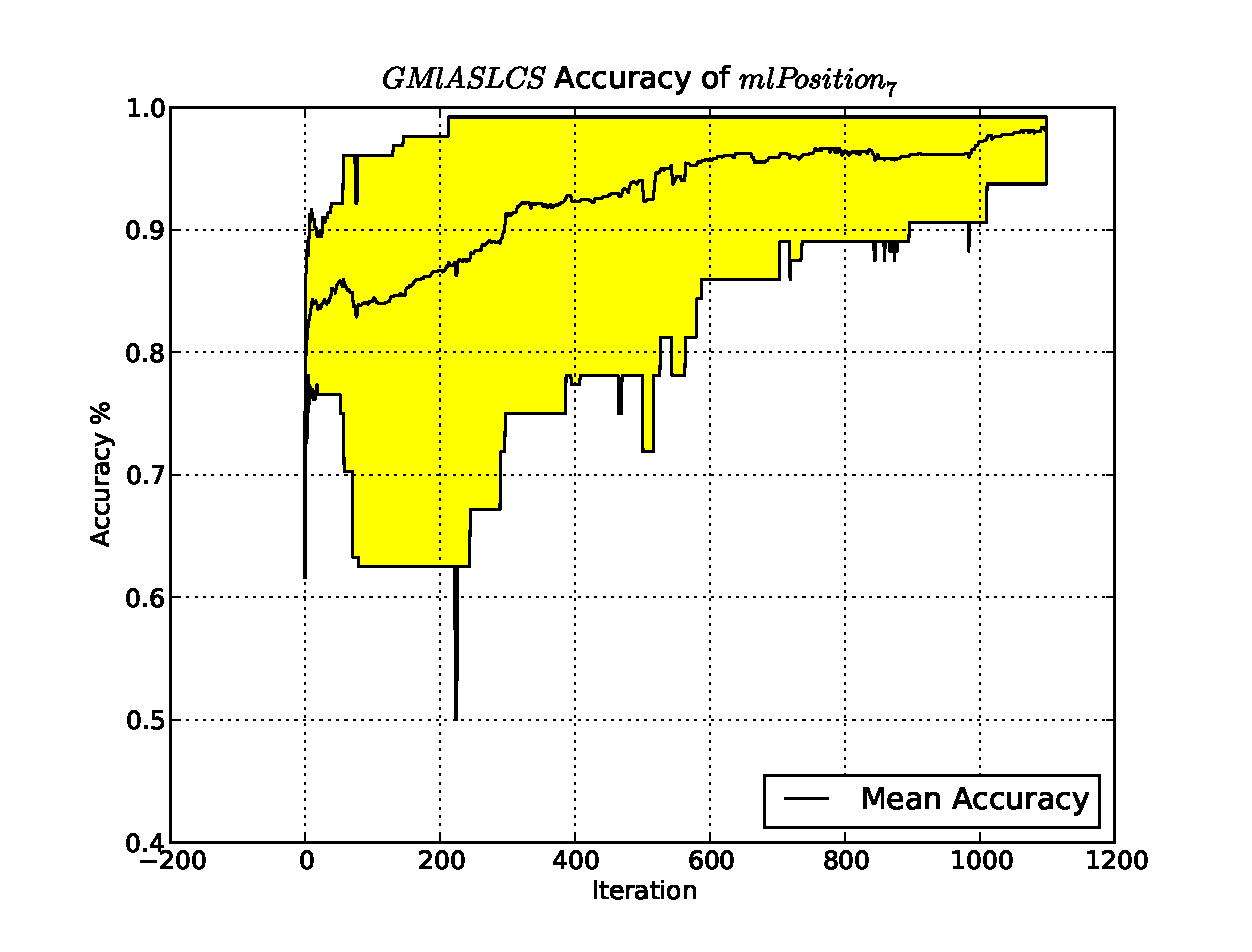
\includegraphics[scale=.49]{./images/artificial/gmlaslcs0/base/mlPosition7GMlASLCSacc.eps}
 
  \centering
  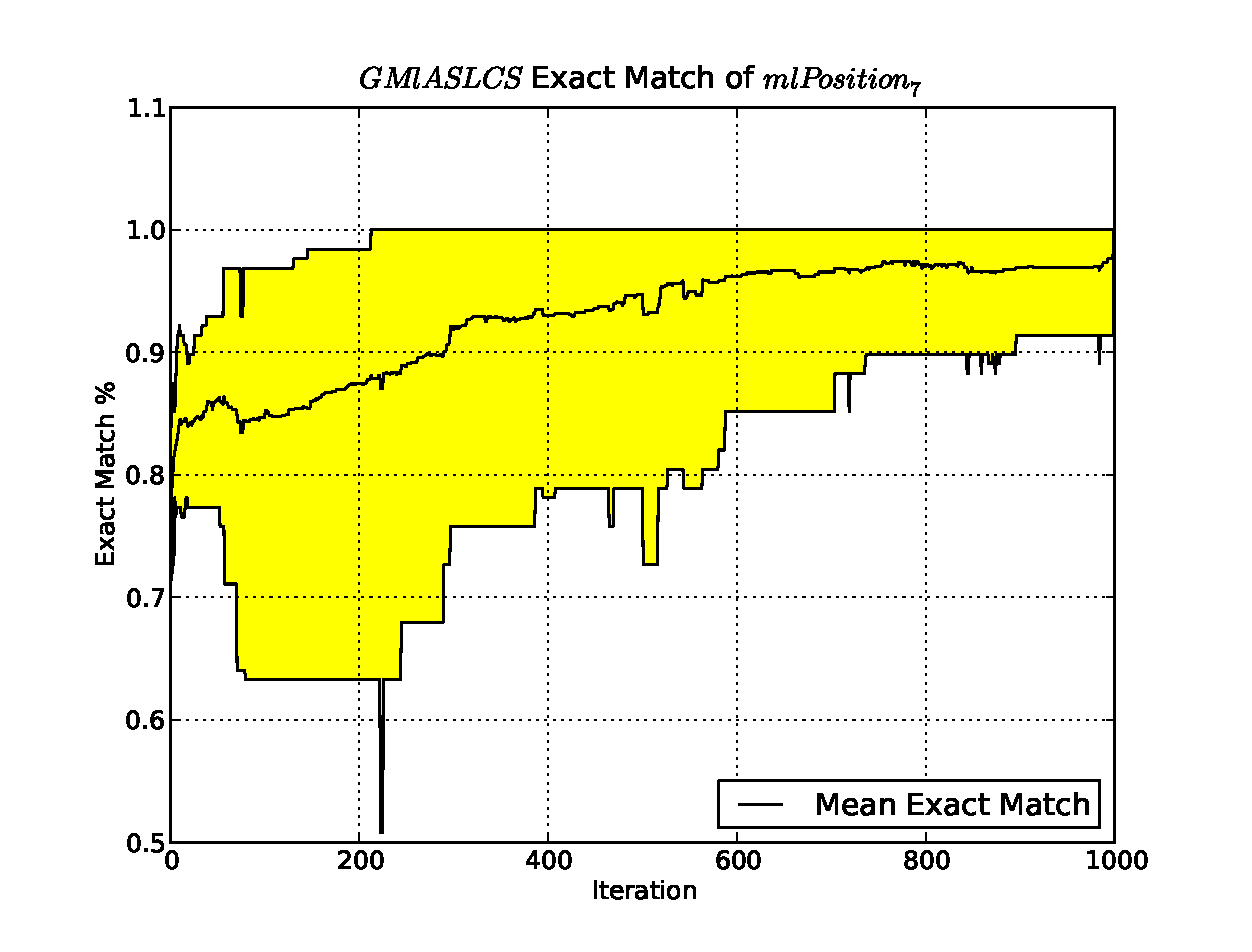
\includegraphics[scale=.49]{./images/artificial/gmlaslcs0/base/mlPosition7GMlASLCSex.eps}
  
  \centering
  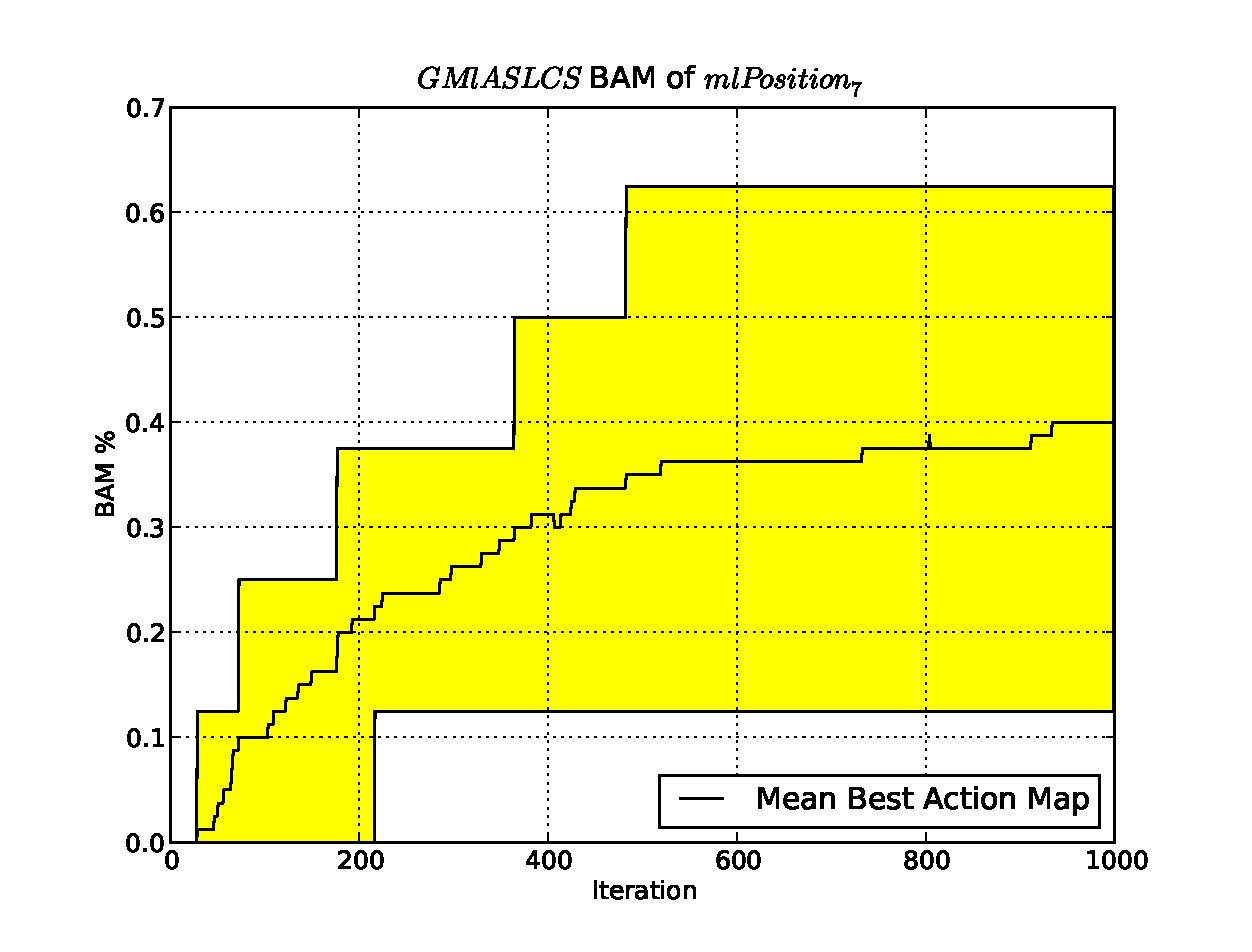
\includegraphics[scale=.49]{./images/artificial/gmlaslcs0/base/mlPosition7GMlASLCSbam.eps}
\end{figure}


\begin{figure}[ht]
  \caption{Διαγράμματα χαρτογράφησης $mlIdentity_{7}$ του GMl-ASLCS$_{\:0}$.}
  \label{fig:gmlaslcs0Identity7}
  \centering
  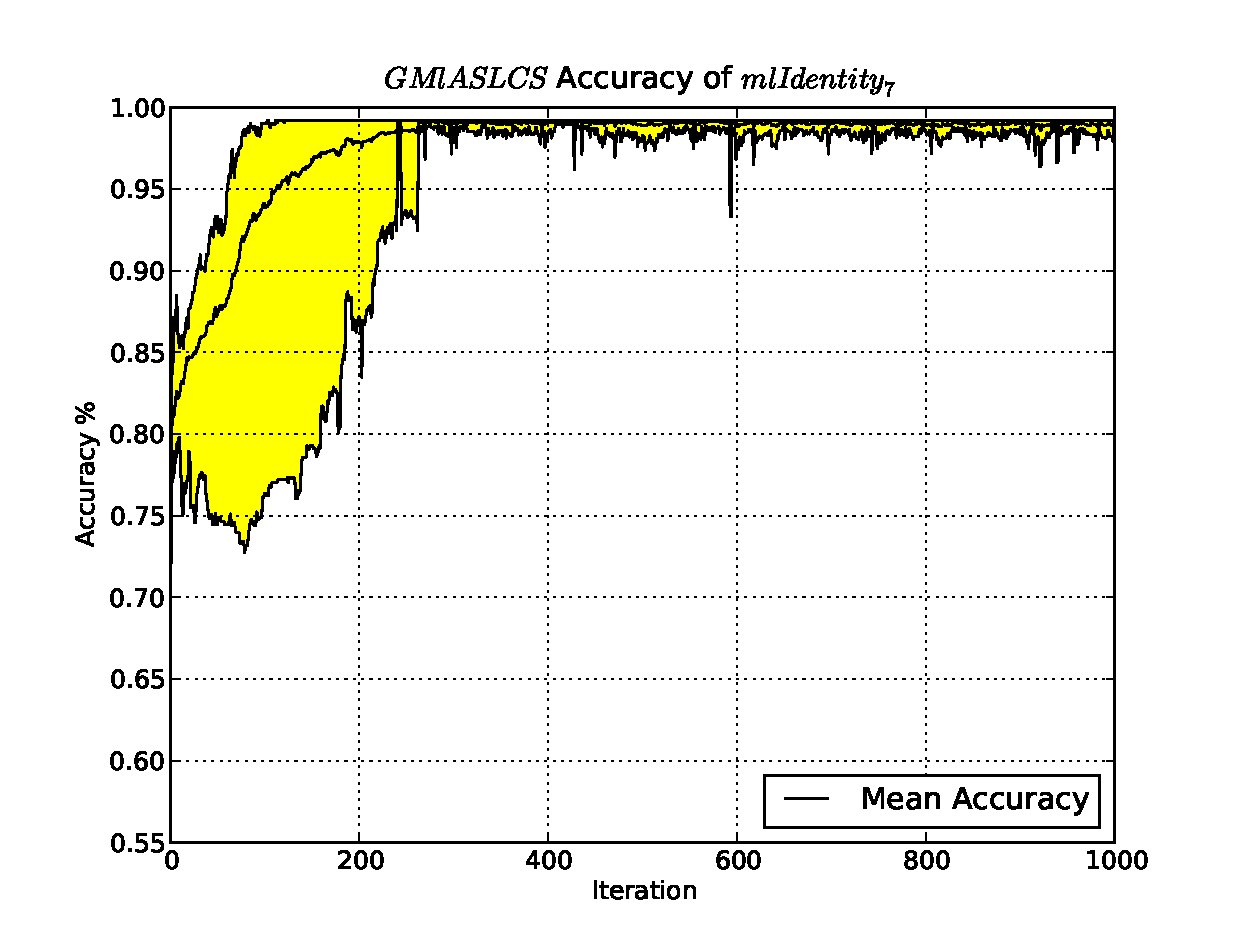
\includegraphics[scale=.49]{./images/artificial/gmlaslcs0/base/mlIdentity7GMlASLCSacc.eps}
  
  
  \centering
  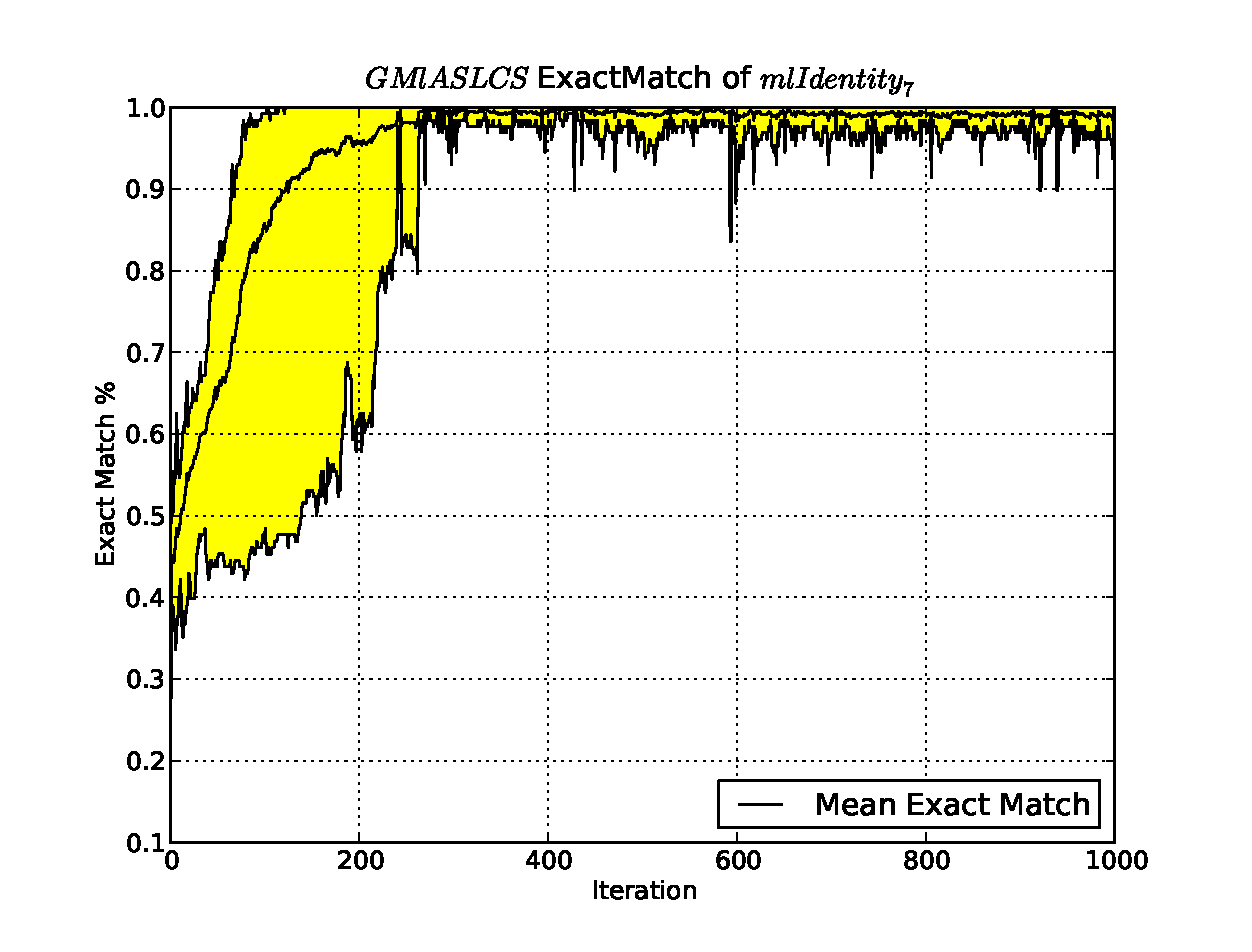
\includegraphics[scale=.49]{./images/artificial/gmlaslcs0/base/mlIdentity7GMlASLCSex.eps}

  \centering
  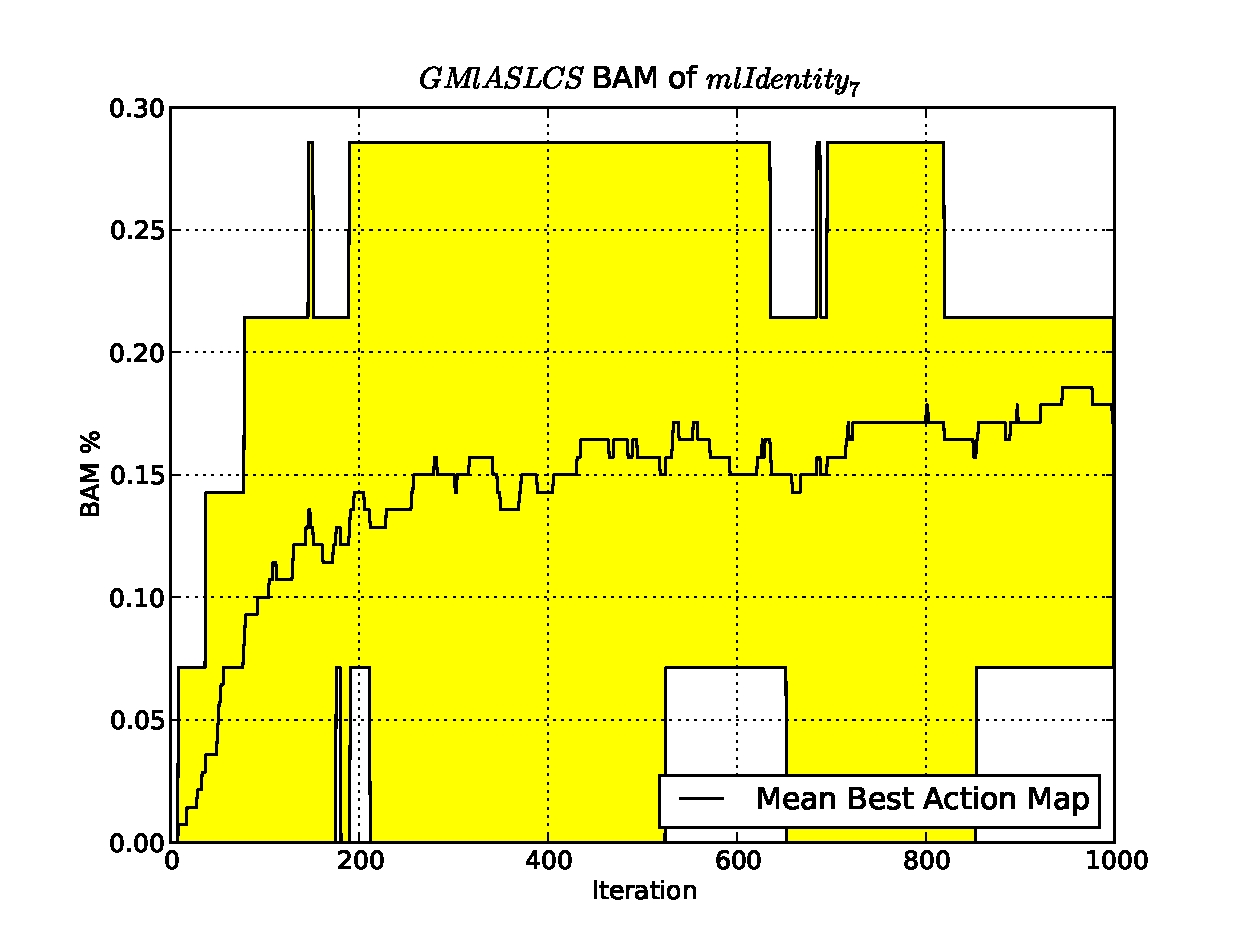
\includegraphics[scale=.49]{./images/artificial/gmlaslcs0/base/mlIdentity7GMlASLCSbam.eps}
\end{figure}


\begin{figure}[ht]
  \caption{Διαγράμματα χαρτογράφησης $adder_{7}^{3}$ του GMl-ASLCS$_{\:0}$.}
  \label{fig:gmlaslcs0adder7_3}
  \begin{minipage}[b]{0.5\linewidth}
  	\centering
  	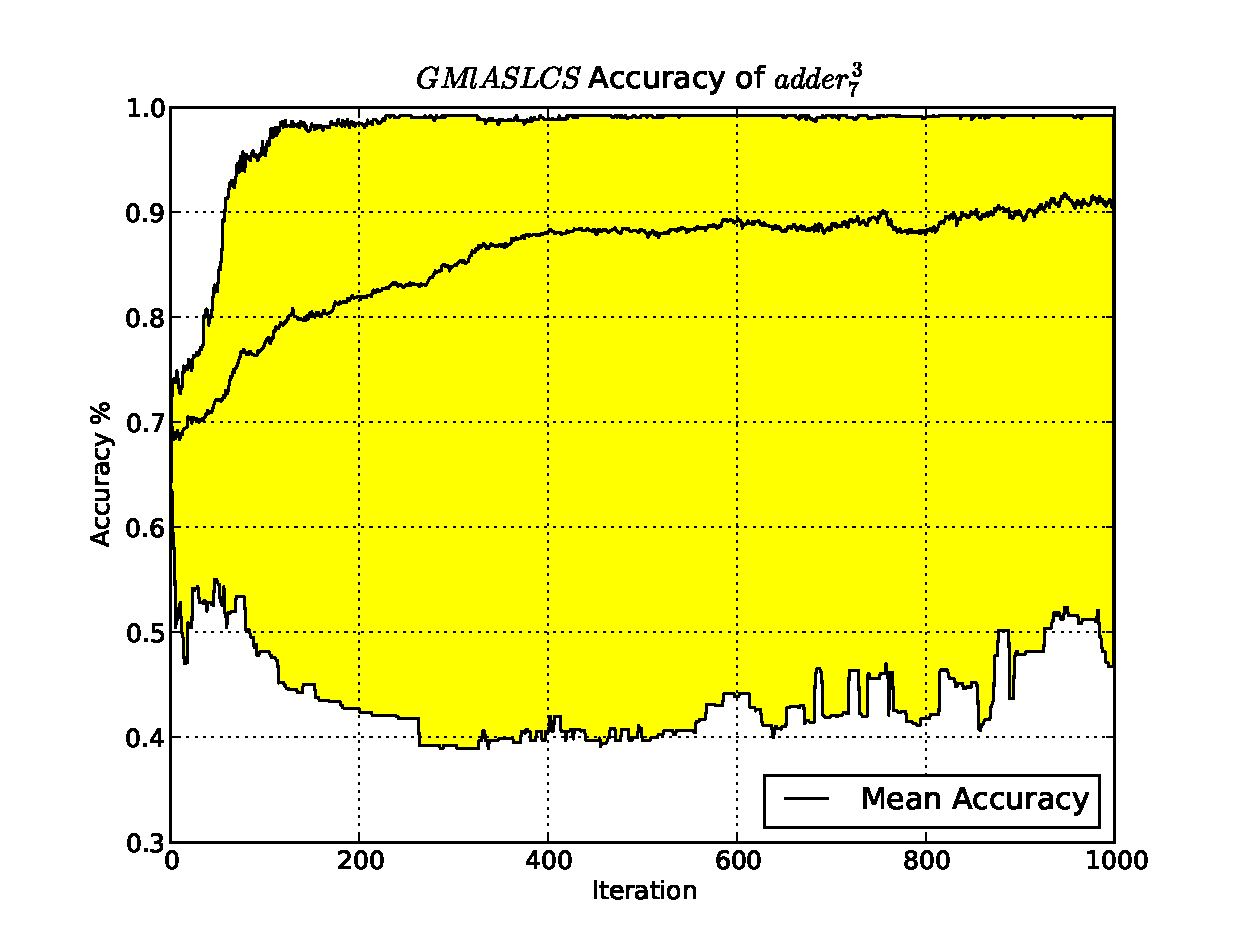
\includegraphics[scale=.42]{./images/artificial/gmlaslcs0/base/adder7_3GMlASLCSacc.eps}
  \end{minipage}
  \begin{minipage}[b]{0.5\linewidth}
  	\centering
  	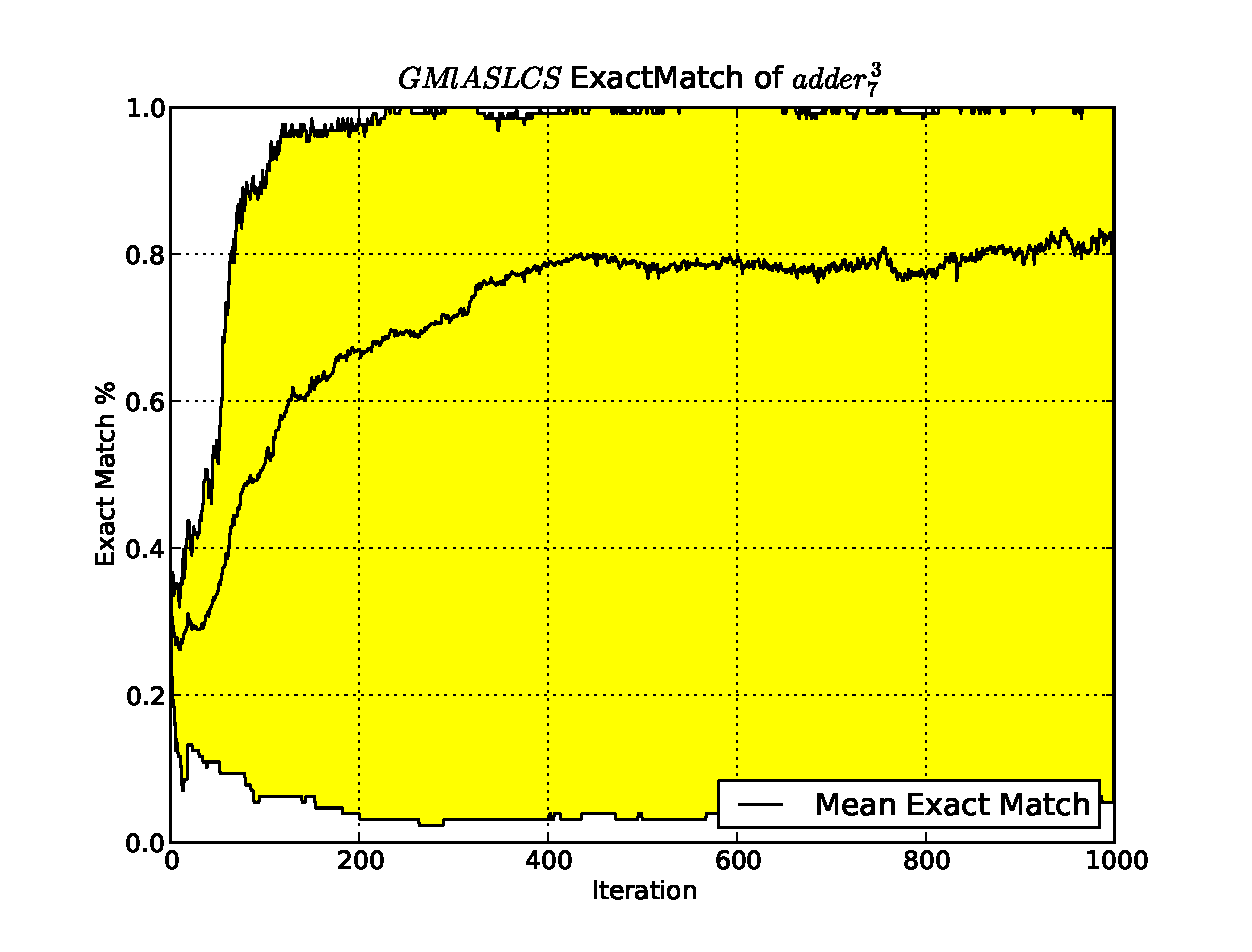
\includegraphics[scale=.42]{./images/artificial/gmlaslcs0/base/adder7_3GMlASLCSex.eps}
  \end{minipage}
\end{figure}

\begin{figure}[ht]
  \caption{Διαγράμματα χαρτογράφησης $adder_{7}^{24}$ του GMl-ASLCS$_{\:0}$.}
  \label{fig:gmlaslcs0adder7_24}
  \begin{minipage}[b]{0.5\linewidth}
    \centering
    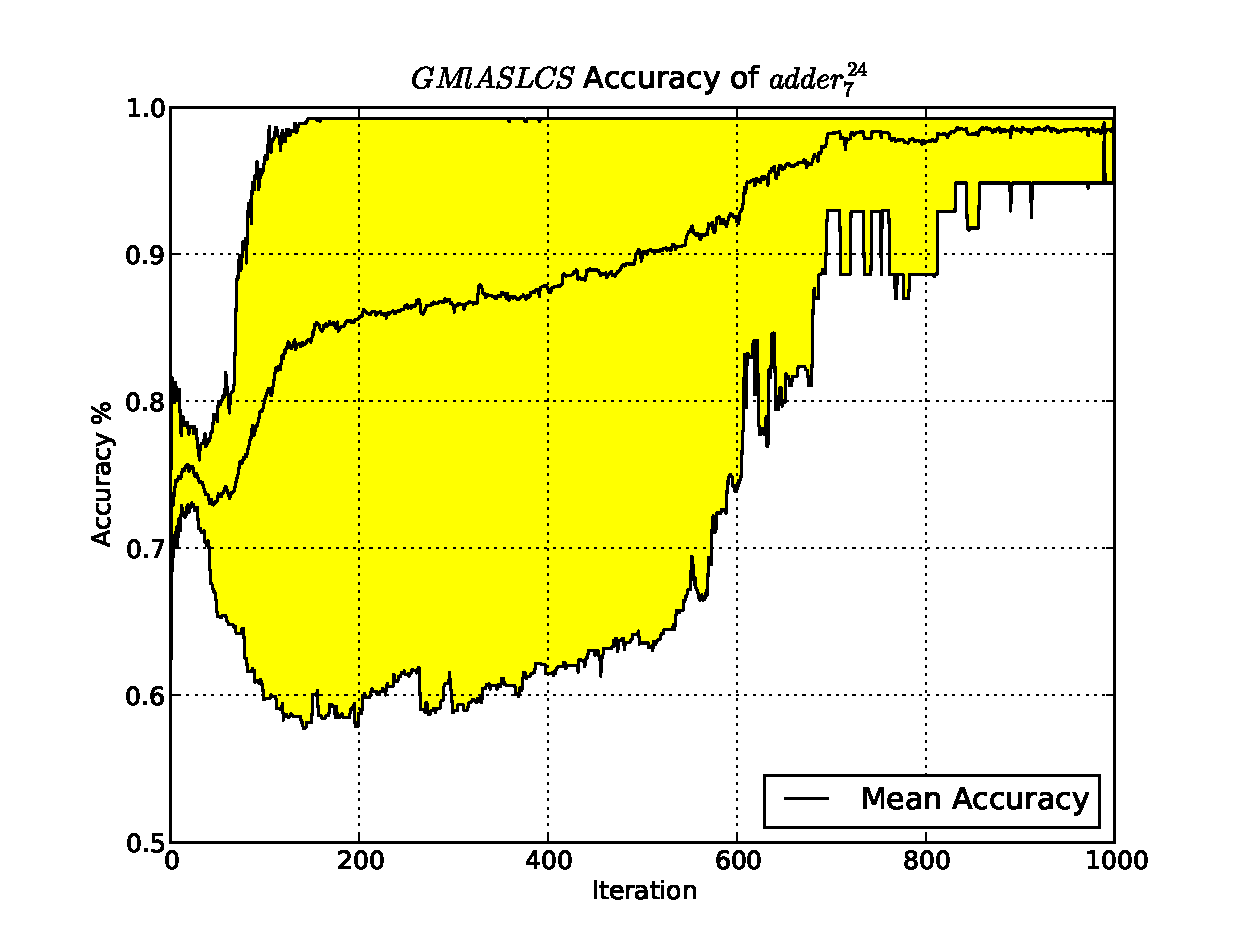
\includegraphics[scale=.42]{./images/artificial/gmlaslcs0/base/adder7_24GMlASLCSacc.eps}
  \end{minipage}
  \begin{minipage}[b]{0.5\linewidth}
    \centering
    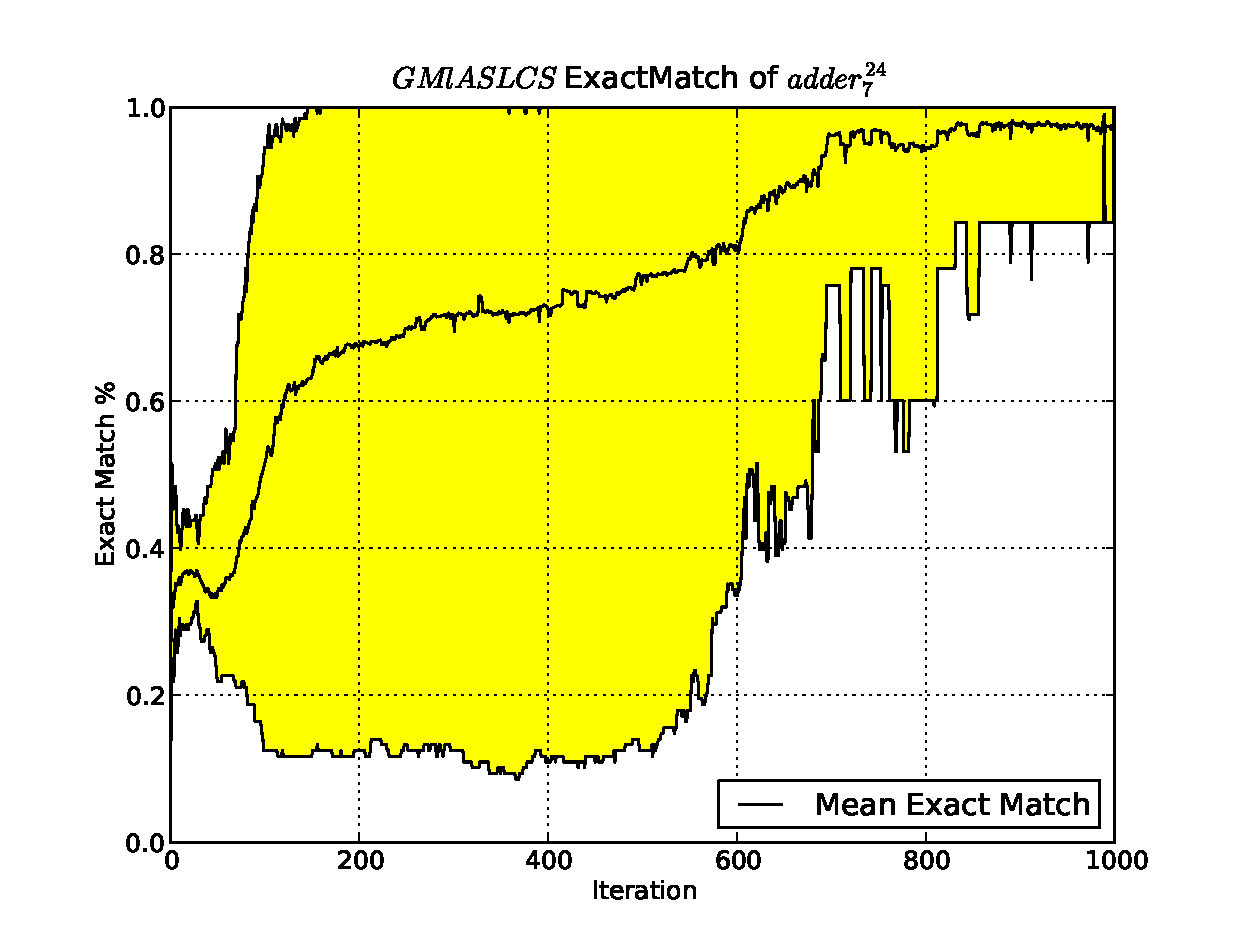
\includegraphics[scale=.42]{./images/artificial/gmlaslcs0/base/adder7_24GMlASLCSex.eps}
  \end{minipage}
\end{figure}

Όσον αφορά στην οικογένεια προβλημάτων $adder_{N}^{k}$, μελετήθηκαν δύο είδη: το $adder_{7}^{3}$ και το $adder_{7}^{24}$. Και τα δύο προβλήματα διαθέτουν την ίδια πολυκατηγορική πληθικότητα. Όμως, το $adder_{7}^{3}$, στο βέλτιστο χάρτη του έχει όλους τους κανόνες ειδικευμένους, ενώ το $adder_{7}^{24}$ έχει έναν ανάμεικτο χάρτη από πλευράς γενίκευσης, με γενικούς κανόνες στα δυαδικά ψηφία χαμηλής σημασίας και ειδικούς στα υψηλής. Σε αυτά τα δύο προβλήματα δε διερευνήθηκε η ικανότητα προσέγγισης του βέλτιστου χάρτη, αφού εξετάζονται οι δύο ακραίες περιπτώσεις ανάπτυξής του με τα προβλήματα $mlPosition_{7}$ και $mlIdentity_{7}$, αλλά μόνο η προβλεπτική ικανότητα.


%-----------------------------------------position-----------------------------------------%


\subsection{Οι τροποποιημένοι αλγόριθμοι GMl-ASLCS$_{\:0*}$ στο πρόβλημα $mlPosition_{7}$}
Τα Σχήματα \ref{fig:gmlaslcs0DPosition7}, \ref{fig:gmlaslcs0GAPosition7}, \ref{fig:gmlaslcs0MPosition7} και \ref{fig:gmlaslcs0CPosition7} παρουσιάζουν την εξέλιξη των μετρικών της Ακρίβειας, της Ακριβούς Ορθότητας και του ποσοστού κάλυψης του ΧΒΑ για το σύνολο δεδομένων $mlPosition_{7}$, των ΜαΣΤ GMl-ASLCS$_{\:0D}$, GMl-ASLCS$_{\:0GA}$, GMl-ASLCS$_{\:0M}$ και GMl-ASLCS$_{\:0C}$, αντίστοιχα.


\begin{figure}[ht]
  \caption{Διαγράμματα χαρτογράφησης $mlPosition_{7}$ του GMl-ASLCS$_{\:0D}$.}
  \label{fig:gmlaslcs0DPosition7}
  \centering
  \scalebox{0.49}{\Large% GNUPLOT: LaTeX picture with Postscript
\begingroup
  \makeatletter
  \providecommand\color[2][]{%
    \GenericError{(gnuplot) \space\space\space\@spaces}{%
      Package color not loaded in conjunction with
      terminal option `colourtext'%
    }{See the gnuplot documentation for explanation.%
    }{Either use 'blacktext' in gnuplot or load the package
      color.sty in LaTeX.}%
    \renewcommand\color[2][]{}%
  }%
  \providecommand\includegraphics[2][]{%
    \GenericError{(gnuplot) \space\space\space\@spaces}{%
      Package graphicx or graphics not loaded%
    }{See the gnuplot documentation for explanation.%
    }{The gnuplot epslatex terminal needs graphicx.sty or graphics.sty.}%
    \renewcommand\includegraphics[2][]{}%
  }%
  \providecommand\rotatebox[2]{#2}%
  \@ifundefined{ifGPcolor}{%
    \newif\ifGPcolor
    \GPcolorfalse
  }{}%
  \@ifundefined{ifGPblacktext}{%
    \newif\ifGPblacktext
    \GPblacktexttrue
  }{}%
  % define a \g@addto@macro without @ in the name:
  \let\gplgaddtomacro\g@addto@macro
  % define empty templates for all commands taking text:
  \gdef\gplbacktext{}%
  \gdef\gplfronttext{}%
  \makeatother
  \ifGPblacktext
    % no textcolor at all
    \def\colorrgb#1{}%
    \def\colorgray#1{}%
  \else
    % gray or color?
    \ifGPcolor
      \def\colorrgb#1{\color[rgb]{#1}}%
      \def\colorgray#1{\color[gray]{#1}}%
      \expandafter\def\csname LTw\endcsname{\color{white}}%
      \expandafter\def\csname LTb\endcsname{\color{black}}%
      \expandafter\def\csname LTa\endcsname{\color{black}}%
      \expandafter\def\csname LT0\endcsname{\color[rgb]{1,0,0}}%
      \expandafter\def\csname LT1\endcsname{\color[rgb]{0,1,0}}%
      \expandafter\def\csname LT2\endcsname{\color[rgb]{0,0,1}}%
      \expandafter\def\csname LT3\endcsname{\color[rgb]{1,0,1}}%
      \expandafter\def\csname LT4\endcsname{\color[rgb]{0,1,1}}%
      \expandafter\def\csname LT5\endcsname{\color[rgb]{1,1,0}}%
      \expandafter\def\csname LT6\endcsname{\color[rgb]{0,0,0}}%
      \expandafter\def\csname LT7\endcsname{\color[rgb]{1,0.3,0}}%
      \expandafter\def\csname LT8\endcsname{\color[rgb]{0.5,0.5,0.5}}%
    \else
      % gray
      \def\colorrgb#1{\color{black}}%
      \def\colorgray#1{\color[gray]{#1}}%
      \expandafter\def\csname LTw\endcsname{\color{white}}%
      \expandafter\def\csname LTb\endcsname{\color{black}}%
      \expandafter\def\csname LTa\endcsname{\color{black}}%
      \expandafter\def\csname LT0\endcsname{\color{black}}%
      \expandafter\def\csname LT1\endcsname{\color{black}}%
      \expandafter\def\csname LT2\endcsname{\color{black}}%
      \expandafter\def\csname LT3\endcsname{\color{black}}%
      \expandafter\def\csname LT4\endcsname{\color{black}}%
      \expandafter\def\csname LT5\endcsname{\color{black}}%
      \expandafter\def\csname LT6\endcsname{\color{black}}%
      \expandafter\def\csname LT7\endcsname{\color{black}}%
      \expandafter\def\csname LT8\endcsname{\color{black}}%
    \fi
  \fi
  \setlength{\unitlength}{0.0500bp}%
  \begin{picture}(11520.00,8640.00)%
    \gplgaddtomacro\gplbacktext{%
    }%
    \gplgaddtomacro\gplfronttext{%
      \csname LTb\endcsname%
      \put(8569,8377){\makebox(0,0)[r]{\strut{}$GMl-ASLCS_{\:0D} \: mean \: accuracy \: in \: mlPosition_7$}}%
      \colorrgb{0.00,0.00,0.00}%
      \put(1257,950){\makebox(0,0)[r]{\strut{}$0$}}%
      \colorrgb{0.00,0.00,0.00}%
      \put(1257,2294){\makebox(0,0)[r]{\strut{}$0.2$}}%
      \colorrgb{0.00,0.00,0.00}%
      \put(1257,3637){\makebox(0,0)[r]{\strut{}$0.4$}}%
      \colorrgb{0.00,0.00,0.00}%
      \put(1257,4981){\makebox(0,0)[r]{\strut{}$0.6$}}%
      \colorrgb{0.00,0.00,0.00}%
      \put(1257,6324){\makebox(0,0)[r]{\strut{}$0.8$}}%
      \colorrgb{0.00,0.00,0.00}%
      \put(1257,7668){\makebox(0,0)[r]{\strut{}$1$}}%
      \colorrgb{0.00,0.00,0.00}%
      \put(1497,550){\makebox(0,0){\strut{}$0$}}%
      \colorrgb{0.00,0.00,0.00}%
      \put(3120,550){\makebox(0,0){\strut{}$200$}}%
      \colorrgb{0.00,0.00,0.00}%
      \put(4743,550){\makebox(0,0){\strut{}$400$}}%
      \colorrgb{0.00,0.00,0.00}%
      \put(6366,550){\makebox(0,0){\strut{}$600$}}%
      \colorrgb{0.00,0.00,0.00}%
      \put(7989,550){\makebox(0,0){\strut{}$800$}}%
      \colorrgb{0.00,0.00,0.00}%
      \put(9612,550){\makebox(0,0){\strut{}$1000$}}%
    }%
    \gplbacktext
    \put(0,0){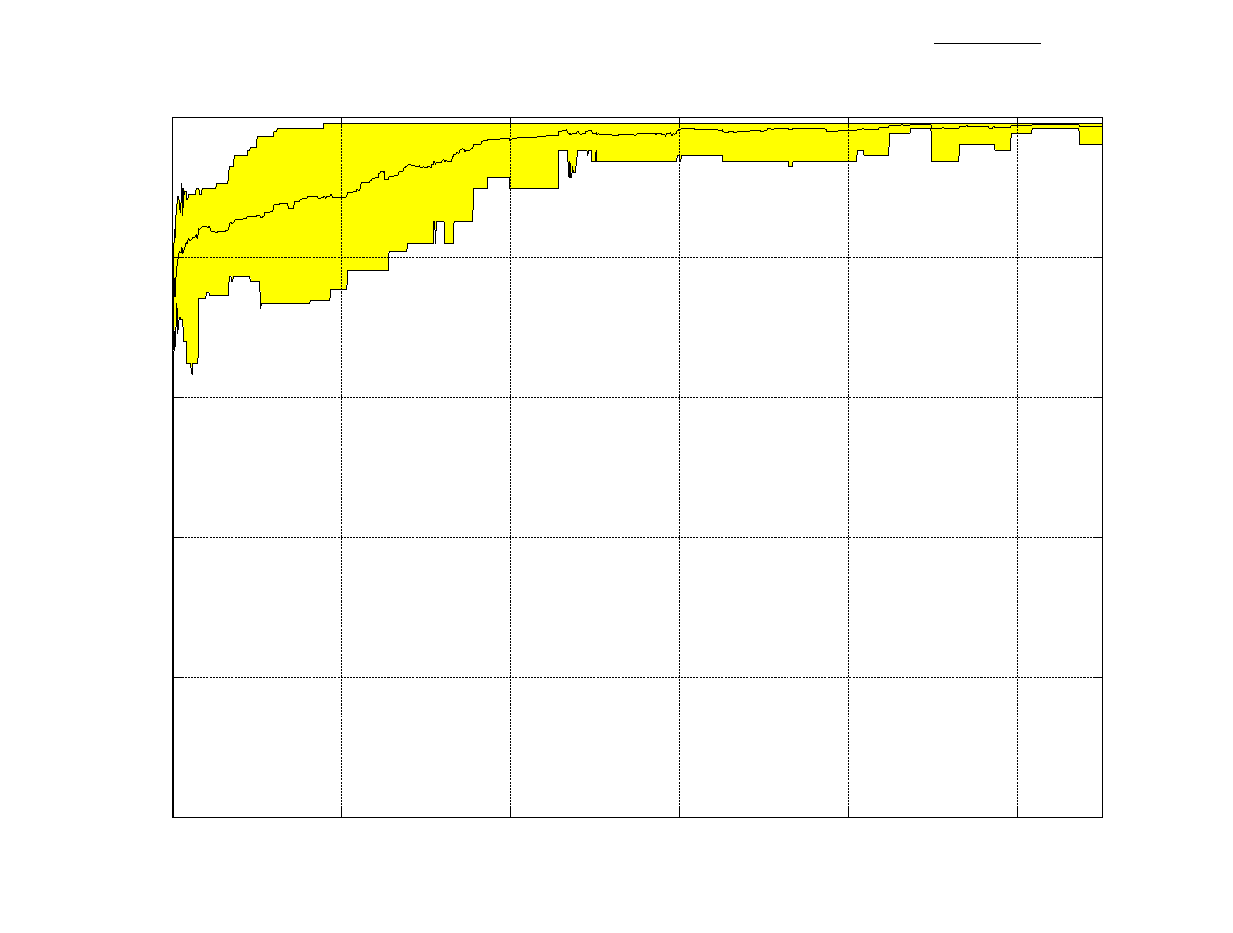
\includegraphics{./images/artificial/gmlaslcs0/positionDacc.eps}}%
    \gplfronttext
  \end{picture}%
\endgroup
}
  \put(-285,70){\rotatebox{90}{$Accuracy$}}
  \scalebox{0.8}{\put(-200,0){\rotatebox{0}{$iterations$}}}
  \label{fig:gmlaslcs0DPosition7Acc} 
  
  \centering
  \scalebox{0.49}{\Large% GNUPLOT: LaTeX picture with Postscript
\begingroup
  \makeatletter
  \providecommand\color[2][]{%
    \GenericError{(gnuplot) \space\space\space\@spaces}{%
      Package color not loaded in conjunction with
      terminal option `colourtext'%
    }{See the gnuplot documentation for explanation.%
    }{Either use 'blacktext' in gnuplot or load the package
      color.sty in LaTeX.}%
    \renewcommand\color[2][]{}%
  }%
  \providecommand\includegraphics[2][]{%
    \GenericError{(gnuplot) \space\space\space\@spaces}{%
      Package graphicx or graphics not loaded%
    }{See the gnuplot documentation for explanation.%
    }{The gnuplot epslatex terminal needs graphicx.sty or graphics.sty.}%
    \renewcommand\includegraphics[2][]{}%
  }%
  \providecommand\rotatebox[2]{#2}%
  \@ifundefined{ifGPcolor}{%
    \newif\ifGPcolor
    \GPcolorfalse
  }{}%
  \@ifundefined{ifGPblacktext}{%
    \newif\ifGPblacktext
    \GPblacktexttrue
  }{}%
  % define a \g@addto@macro without @ in the name:
  \let\gplgaddtomacro\g@addto@macro
  % define empty templates for all commands taking text:
  \gdef\gplbacktext{}%
  \gdef\gplfronttext{}%
  \makeatother
  \ifGPblacktext
    % no textcolor at all
    \def\colorrgb#1{}%
    \def\colorgray#1{}%
  \else
    % gray or color?
    \ifGPcolor
      \def\colorrgb#1{\color[rgb]{#1}}%
      \def\colorgray#1{\color[gray]{#1}}%
      \expandafter\def\csname LTw\endcsname{\color{white}}%
      \expandafter\def\csname LTb\endcsname{\color{black}}%
      \expandafter\def\csname LTa\endcsname{\color{black}}%
      \expandafter\def\csname LT0\endcsname{\color[rgb]{1,0,0}}%
      \expandafter\def\csname LT1\endcsname{\color[rgb]{0,1,0}}%
      \expandafter\def\csname LT2\endcsname{\color[rgb]{0,0,1}}%
      \expandafter\def\csname LT3\endcsname{\color[rgb]{1,0,1}}%
      \expandafter\def\csname LT4\endcsname{\color[rgb]{0,1,1}}%
      \expandafter\def\csname LT5\endcsname{\color[rgb]{1,1,0}}%
      \expandafter\def\csname LT6\endcsname{\color[rgb]{0,0,0}}%
      \expandafter\def\csname LT7\endcsname{\color[rgb]{1,0.3,0}}%
      \expandafter\def\csname LT8\endcsname{\color[rgb]{0.5,0.5,0.5}}%
    \else
      % gray
      \def\colorrgb#1{\color{black}}%
      \def\colorgray#1{\color[gray]{#1}}%
      \expandafter\def\csname LTw\endcsname{\color{white}}%
      \expandafter\def\csname LTb\endcsname{\color{black}}%
      \expandafter\def\csname LTa\endcsname{\color{black}}%
      \expandafter\def\csname LT0\endcsname{\color{black}}%
      \expandafter\def\csname LT1\endcsname{\color{black}}%
      \expandafter\def\csname LT2\endcsname{\color{black}}%
      \expandafter\def\csname LT3\endcsname{\color{black}}%
      \expandafter\def\csname LT4\endcsname{\color{black}}%
      \expandafter\def\csname LT5\endcsname{\color{black}}%
      \expandafter\def\csname LT6\endcsname{\color{black}}%
      \expandafter\def\csname LT7\endcsname{\color{black}}%
      \expandafter\def\csname LT8\endcsname{\color{black}}%
    \fi
  \fi
  \setlength{\unitlength}{0.0500bp}%
  \begin{picture}(11520.00,8640.00)%
    \gplgaddtomacro\gplbacktext{%
    }%
    \gplgaddtomacro\gplfronttext{%
      \csname LTb\endcsname%
      \put(8929,8377){\makebox(0,0)[r]{\strut{}$GMl-ASLCS_{\:0D} \: mean \: exact  \:match \: in  \:mlPosition_7$}}%
      \colorrgb{0.00,0.00,0.00}%
      \put(1257,950){\makebox(0,0)[r]{\strut{}$0$}}%
      \colorrgb{0.00,0.00,0.00}%
      \put(1257,2294){\makebox(0,0)[r]{\strut{}$0.2$}}%
      \colorrgb{0.00,0.00,0.00}%
      \put(1257,3637){\makebox(0,0)[r]{\strut{}$0.4$}}%
      \colorrgb{0.00,0.00,0.00}%
      \put(1257,4981){\makebox(0,0)[r]{\strut{}$0.6$}}%
      \colorrgb{0.00,0.00,0.00}%
      \put(1257,6324){\makebox(0,0)[r]{\strut{}$0.8$}}%
      \colorrgb{0.00,0.00,0.00}%
      \put(1257,7668){\makebox(0,0)[r]{\strut{}$1$}}%
      \colorrgb{0.00,0.00,0.00}%
      \put(1497,550){\makebox(0,0){\strut{}$0$}}%
      \colorrgb{0.00,0.00,0.00}%
      \put(3120,550){\makebox(0,0){\strut{}$200$}}%
      \colorrgb{0.00,0.00,0.00}%
      \put(4743,550){\makebox(0,0){\strut{}$400$}}%
      \colorrgb{0.00,0.00,0.00}%
      \put(6366,550){\makebox(0,0){\strut{}$600$}}%
      \colorrgb{0.00,0.00,0.00}%
      \put(7989,550){\makebox(0,0){\strut{}$800$}}%
      \colorrgb{0.00,0.00,0.00}%
      \put(9612,550){\makebox(0,0){\strut{}$1000$}}%
    }%
    \gplbacktext
    \put(0,0){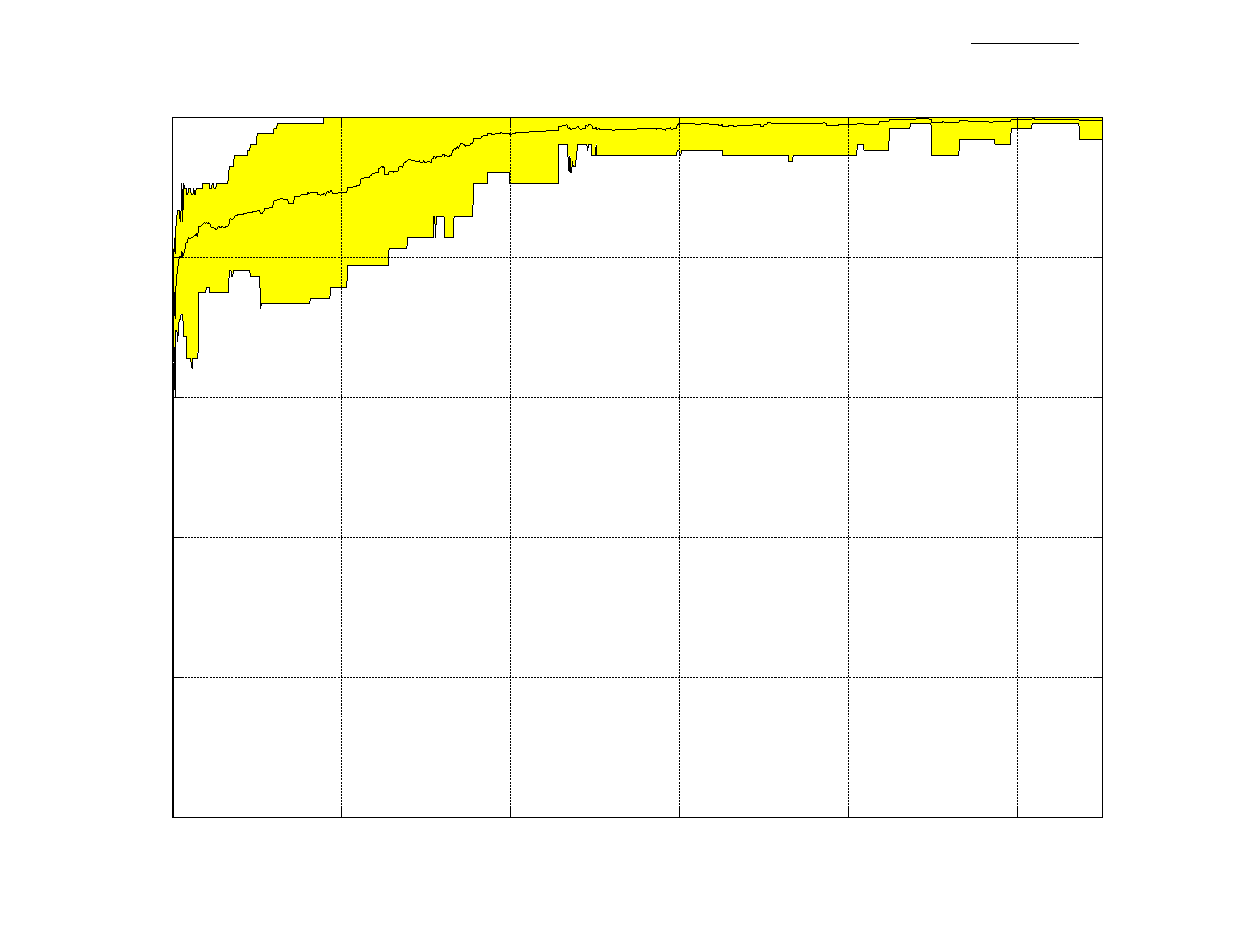
\includegraphics{./images/artificial/gmlaslcs0/positionDex.eps}}%
    \gplfronttext
  \end{picture}%
\endgroup
}
  \put(-285,70){\rotatebox{90}{$Exact \: Match$}}
  \scalebox{0.8}{\put(-200,0){\rotatebox{0}{$iterations$}}}
  \label{fig:gmlaslcs0DPosition7Ex}  
   
  \centering
  \scalebox{0.49}{\Large% GNUPLOT: LaTeX picture with Postscript
\begingroup
  \makeatletter
  \providecommand\color[2][]{%
    \GenericError{(gnuplot) \space\space\space\@spaces}{%
      Package color not loaded in conjunction with
      terminal option `colourtext'%
    }{See the gnuplot documentation for explanation.%
    }{Either use 'blacktext' in gnuplot or load the package
      color.sty in LaTeX.}%
    \renewcommand\color[2][]{}%
  }%
  \providecommand\includegraphics[2][]{%
    \GenericError{(gnuplot) \space\space\space\@spaces}{%
      Package graphicx or graphics not loaded%
    }{See the gnuplot documentation for explanation.%
    }{The gnuplot epslatex terminal needs graphicx.sty or graphics.sty.}%
    \renewcommand\includegraphics[2][]{}%
  }%
  \providecommand\rotatebox[2]{#2}%
  \@ifundefined{ifGPcolor}{%
    \newif\ifGPcolor
    \GPcolorfalse
  }{}%
  \@ifundefined{ifGPblacktext}{%
    \newif\ifGPblacktext
    \GPblacktexttrue
  }{}%
  % define a \g@addto@macro without @ in the name:
  \let\gplgaddtomacro\g@addto@macro
  % define empty templates for all commands taking text:
  \gdef\gplbacktext{}%
  \gdef\gplfronttext{}%
  \makeatother
  \ifGPblacktext
    % no textcolor at all
    \def\colorrgb#1{}%
    \def\colorgray#1{}%
  \else
    % gray or color?
    \ifGPcolor
      \def\colorrgb#1{\color[rgb]{#1}}%
      \def\colorgray#1{\color[gray]{#1}}%
      \expandafter\def\csname LTw\endcsname{\color{white}}%
      \expandafter\def\csname LTb\endcsname{\color{black}}%
      \expandafter\def\csname LTa\endcsname{\color{black}}%
      \expandafter\def\csname LT0\endcsname{\color[rgb]{1,0,0}}%
      \expandafter\def\csname LT1\endcsname{\color[rgb]{0,1,0}}%
      \expandafter\def\csname LT2\endcsname{\color[rgb]{0,0,1}}%
      \expandafter\def\csname LT3\endcsname{\color[rgb]{1,0,1}}%
      \expandafter\def\csname LT4\endcsname{\color[rgb]{0,1,1}}%
      \expandafter\def\csname LT5\endcsname{\color[rgb]{1,1,0}}%
      \expandafter\def\csname LT6\endcsname{\color[rgb]{0,0,0}}%
      \expandafter\def\csname LT7\endcsname{\color[rgb]{1,0.3,0}}%
      \expandafter\def\csname LT8\endcsname{\color[rgb]{0.5,0.5,0.5}}%
    \else
      % gray
      \def\colorrgb#1{\color{black}}%
      \def\colorgray#1{\color[gray]{#1}}%
      \expandafter\def\csname LTw\endcsname{\color{white}}%
      \expandafter\def\csname LTb\endcsname{\color{black}}%
      \expandafter\def\csname LTa\endcsname{\color{black}}%
      \expandafter\def\csname LT0\endcsname{\color{black}}%
      \expandafter\def\csname LT1\endcsname{\color{black}}%
      \expandafter\def\csname LT2\endcsname{\color{black}}%
      \expandafter\def\csname LT3\endcsname{\color{black}}%
      \expandafter\def\csname LT4\endcsname{\color{black}}%
      \expandafter\def\csname LT5\endcsname{\color{black}}%
      \expandafter\def\csname LT6\endcsname{\color{black}}%
      \expandafter\def\csname LT7\endcsname{\color{black}}%
      \expandafter\def\csname LT8\endcsname{\color{black}}%
    \fi
  \fi
  \setlength{\unitlength}{0.0500bp}%
  \begin{picture}(11520.00,8640.00)%
    \gplgaddtomacro\gplbacktext{%
    }%
    \gplgaddtomacro\gplfronttext{%
      \csname LTb\endcsname%
      \put(9049,8377){\makebox(0,0)[r]{\strut{}$GMl-ASLCS_{\:0D} \: mean \: BAM \: coverage \: in  \:mlPosition_7$}}%
      \colorrgb{0.00,0.00,0.00}%
      \put(1257,950){\makebox(0,0)[r]{\strut{}$0$}}%
      \colorrgb{0.00,0.00,0.00}%
      \put(1257,1790){\makebox(0,0)[r]{\strut{}$0.1$}}%
      \colorrgb{0.00,0.00,0.00}%
      \put(1257,2630){\makebox(0,0)[r]{\strut{}$0.2$}}%
      \colorrgb{0.00,0.00,0.00}%
      \put(1257,3469){\makebox(0,0)[r]{\strut{}$0.3$}}%
      \colorrgb{0.00,0.00,0.00}%
      \put(1257,4309){\makebox(0,0)[r]{\strut{}$0.4$}}%
      \colorrgb{0.00,0.00,0.00}%
      \put(1257,5149){\makebox(0,0)[r]{\strut{}$0.5$}}%
      \colorrgb{0.00,0.00,0.00}%
      \put(1257,5988){\makebox(0,0)[r]{\strut{}$0.6$}}%
      \colorrgb{0.00,0.00,0.00}%
      \put(1257,6828){\makebox(0,0)[r]{\strut{}$0.7$}}%
      \colorrgb{0.00,0.00,0.00}%
      \put(1257,7668){\makebox(0,0)[r]{\strut{}$0.8$}}%
      \colorrgb{0.00,0.00,0.00}%
      \put(1497,550){\makebox(0,0){\strut{}$0$}}%
      \colorrgb{0.00,0.00,0.00}%
      \put(3120,550){\makebox(0,0){\strut{}$200$}}%
      \colorrgb{0.00,0.00,0.00}%
      \put(4743,550){\makebox(0,0){\strut{}$400$}}%
      \colorrgb{0.00,0.00,0.00}%
      \put(6366,550){\makebox(0,0){\strut{}$600$}}%
      \colorrgb{0.00,0.00,0.00}%
      \put(7989,550){\makebox(0,0){\strut{}$800$}}%
      \colorrgb{0.00,0.00,0.00}%
      \put(9612,550){\makebox(0,0){\strut{}$1000$}}%
    }%
    \gplbacktext
    \put(0,0){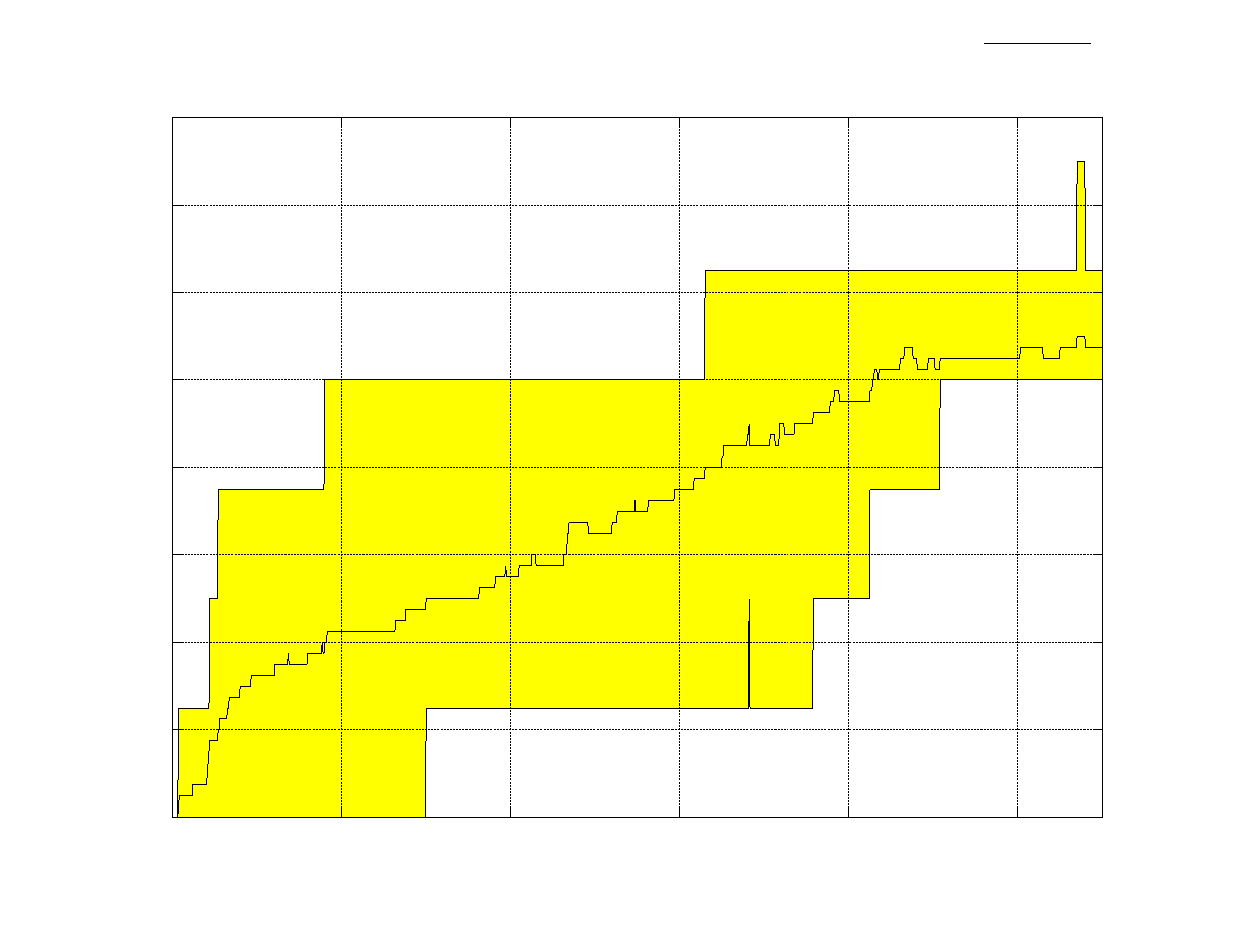
\includegraphics{./images/artificial/gmlaslcs0/positionDBAM.eps}}%
    \gplfronttext
  \end{picture}%
\endgroup
}
  \put(-285,80){\rotatebox{90}{$BAM$}}
  \scalebox{0.8}{\put(-200,0){\rotatebox{0}{$iterations$}}}
  \label{fig:gmlaslcs0DPosition7BAM} 
\end{figure}

\begin{figure}[ht]
  \caption{Διαγράμματα χαρτογράφησης $mlPosition_{7}$ του GMl-ASLCS$_{\:0GA}$.}
  \label{fig:gmlaslcs0GAPosition7}
  \centering
  \scalebox{0.49}{\Large% GNUPLOT: LaTeX picture with Postscript
\begingroup
  \makeatletter
  \providecommand\color[2][]{%
    \GenericError{(gnuplot) \space\space\space\@spaces}{%
      Package color not loaded in conjunction with
      terminal option `colourtext'%
    }{See the gnuplot documentation for explanation.%
    }{Either use 'blacktext' in gnuplot or load the package
      color.sty in LaTeX.}%
    \renewcommand\color[2][]{}%
  }%
  \providecommand\includegraphics[2][]{%
    \GenericError{(gnuplot) \space\space\space\@spaces}{%
      Package graphicx or graphics not loaded%
    }{See the gnuplot documentation for explanation.%
    }{The gnuplot epslatex terminal needs graphicx.sty or graphics.sty.}%
    \renewcommand\includegraphics[2][]{}%
  }%
  \providecommand\rotatebox[2]{#2}%
  \@ifundefined{ifGPcolor}{%
    \newif\ifGPcolor
    \GPcolorfalse
  }{}%
  \@ifundefined{ifGPblacktext}{%
    \newif\ifGPblacktext
    \GPblacktexttrue
  }{}%
  % define a \g@addto@macro without @ in the name:
  \let\gplgaddtomacro\g@addto@macro
  % define empty templates for all commands taking text:
  \gdef\gplbacktext{}%
  \gdef\gplfronttext{}%
  \makeatother
  \ifGPblacktext
    % no textcolor at all
    \def\colorrgb#1{}%
    \def\colorgray#1{}%
  \else
    % gray or color?
    \ifGPcolor
      \def\colorrgb#1{\color[rgb]{#1}}%
      \def\colorgray#1{\color[gray]{#1}}%
      \expandafter\def\csname LTw\endcsname{\color{white}}%
      \expandafter\def\csname LTb\endcsname{\color{black}}%
      \expandafter\def\csname LTa\endcsname{\color{black}}%
      \expandafter\def\csname LT0\endcsname{\color[rgb]{1,0,0}}%
      \expandafter\def\csname LT1\endcsname{\color[rgb]{0,1,0}}%
      \expandafter\def\csname LT2\endcsname{\color[rgb]{0,0,1}}%
      \expandafter\def\csname LT3\endcsname{\color[rgb]{1,0,1}}%
      \expandafter\def\csname LT4\endcsname{\color[rgb]{0,1,1}}%
      \expandafter\def\csname LT5\endcsname{\color[rgb]{1,1,0}}%
      \expandafter\def\csname LT6\endcsname{\color[rgb]{0,0,0}}%
      \expandafter\def\csname LT7\endcsname{\color[rgb]{1,0.3,0}}%
      \expandafter\def\csname LT8\endcsname{\color[rgb]{0.5,0.5,0.5}}%
    \else
      % gray
      \def\colorrgb#1{\color{black}}%
      \def\colorgray#1{\color[gray]{#1}}%
      \expandafter\def\csname LTw\endcsname{\color{white}}%
      \expandafter\def\csname LTb\endcsname{\color{black}}%
      \expandafter\def\csname LTa\endcsname{\color{black}}%
      \expandafter\def\csname LT0\endcsname{\color{black}}%
      \expandafter\def\csname LT1\endcsname{\color{black}}%
      \expandafter\def\csname LT2\endcsname{\color{black}}%
      \expandafter\def\csname LT3\endcsname{\color{black}}%
      \expandafter\def\csname LT4\endcsname{\color{black}}%
      \expandafter\def\csname LT5\endcsname{\color{black}}%
      \expandafter\def\csname LT6\endcsname{\color{black}}%
      \expandafter\def\csname LT7\endcsname{\color{black}}%
      \expandafter\def\csname LT8\endcsname{\color{black}}%
    \fi
  \fi
  \setlength{\unitlength}{0.0500bp}%
  \begin{picture}(11520.00,8640.00)%
    \gplgaddtomacro\gplbacktext{%
    }%
    \gplgaddtomacro\gplfronttext{%
      \csname LTb\endcsname%
      \put(8569,8377){\makebox(0,0)[r]{\strut{}$GMl-ASLCS_{\:0GA} \: mean \: accuracy \: in \: mlPosition_7$}}%
      \colorrgb{0.00,0.00,0.00}%
      \put(1257,950){\makebox(0,0)[r]{\strut{}$0$}}%
      \colorrgb{0.00,0.00,0.00}%
      \put(1257,2294){\makebox(0,0)[r]{\strut{}$0.2$}}%
      \colorrgb{0.00,0.00,0.00}%
      \put(1257,3637){\makebox(0,0)[r]{\strut{}$0.4$}}%
      \colorrgb{0.00,0.00,0.00}%
      \put(1257,4981){\makebox(0,0)[r]{\strut{}$0.6$}}%
      \colorrgb{0.00,0.00,0.00}%
      \put(1257,6324){\makebox(0,0)[r]{\strut{}$0.8$}}%
      \colorrgb{0.00,0.00,0.00}%
      \put(1257,7668){\makebox(0,0)[r]{\strut{}$1$}}%
      \colorrgb{0.00,0.00,0.00}%
      \put(1497,550){\makebox(0,0){\strut{}$0$}}%
      \colorrgb{0.00,0.00,0.00}%
      \put(3120,550){\makebox(0,0){\strut{}$200$}}%
      \colorrgb{0.00,0.00,0.00}%
      \put(4743,550){\makebox(0,0){\strut{}$400$}}%
      \colorrgb{0.00,0.00,0.00}%
      \put(6366,550){\makebox(0,0){\strut{}$600$}}%
      \colorrgb{0.00,0.00,0.00}%
      \put(7989,550){\makebox(0,0){\strut{}$800$}}%
      \colorrgb{0.00,0.00,0.00}%
      \put(9612,550){\makebox(0,0){\strut{}$1000$}}%
    }%
    \gplbacktext
    \put(0,0){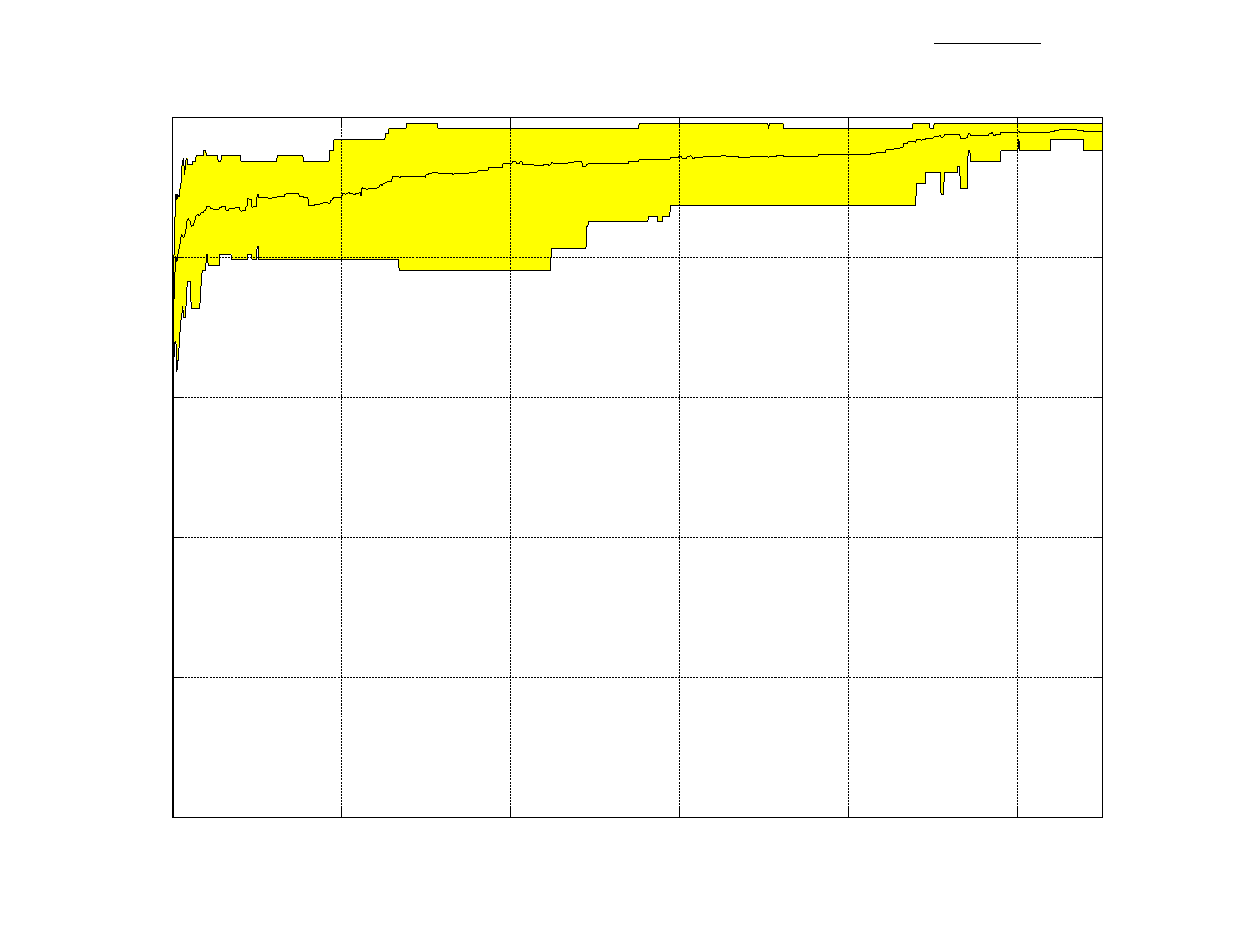
\includegraphics{./images/artificial/gmlaslcs0/positionGAacc.eps}}%
    \gplfronttext
  \end{picture}%
\endgroup
}
  \put(-285,70){\rotatebox{90}{$Accuracy$}}
  \scalebox{0.8}{\put(-200,0){\rotatebox{0}{$iterations$}}}
  \label{fig:gmlaslcs0GAPosition7Acc} 
  
  \centering
  \scalebox{0.49}{\Large% GNUPLOT: LaTeX picture with Postscript
\begingroup
  \makeatletter
  \providecommand\color[2][]{%
    \GenericError{(gnuplot) \space\space\space\@spaces}{%
      Package color not loaded in conjunction with
      terminal option `colourtext'%
    }{See the gnuplot documentation for explanation.%
    }{Either use 'blacktext' in gnuplot or load the package
      color.sty in LaTeX.}%
    \renewcommand\color[2][]{}%
  }%
  \providecommand\includegraphics[2][]{%
    \GenericError{(gnuplot) \space\space\space\@spaces}{%
      Package graphicx or graphics not loaded%
    }{See the gnuplot documentation for explanation.%
    }{The gnuplot epslatex terminal needs graphicx.sty or graphics.sty.}%
    \renewcommand\includegraphics[2][]{}%
  }%
  \providecommand\rotatebox[2]{#2}%
  \@ifundefined{ifGPcolor}{%
    \newif\ifGPcolor
    \GPcolorfalse
  }{}%
  \@ifundefined{ifGPblacktext}{%
    \newif\ifGPblacktext
    \GPblacktexttrue
  }{}%
  % define a \g@addto@macro without @ in the name:
  \let\gplgaddtomacro\g@addto@macro
  % define empty templates for all commands taking text:
  \gdef\gplbacktext{}%
  \gdef\gplfronttext{}%
  \makeatother
  \ifGPblacktext
    % no textcolor at all
    \def\colorrgb#1{}%
    \def\colorgray#1{}%
  \else
    % gray or color?
    \ifGPcolor
      \def\colorrgb#1{\color[rgb]{#1}}%
      \def\colorgray#1{\color[gray]{#1}}%
      \expandafter\def\csname LTw\endcsname{\color{white}}%
      \expandafter\def\csname LTb\endcsname{\color{black}}%
      \expandafter\def\csname LTa\endcsname{\color{black}}%
      \expandafter\def\csname LT0\endcsname{\color[rgb]{1,0,0}}%
      \expandafter\def\csname LT1\endcsname{\color[rgb]{0,1,0}}%
      \expandafter\def\csname LT2\endcsname{\color[rgb]{0,0,1}}%
      \expandafter\def\csname LT3\endcsname{\color[rgb]{1,0,1}}%
      \expandafter\def\csname LT4\endcsname{\color[rgb]{0,1,1}}%
      \expandafter\def\csname LT5\endcsname{\color[rgb]{1,1,0}}%
      \expandafter\def\csname LT6\endcsname{\color[rgb]{0,0,0}}%
      \expandafter\def\csname LT7\endcsname{\color[rgb]{1,0.3,0}}%
      \expandafter\def\csname LT8\endcsname{\color[rgb]{0.5,0.5,0.5}}%
    \else
      % gray
      \def\colorrgb#1{\color{black}}%
      \def\colorgray#1{\color[gray]{#1}}%
      \expandafter\def\csname LTw\endcsname{\color{white}}%
      \expandafter\def\csname LTb\endcsname{\color{black}}%
      \expandafter\def\csname LTa\endcsname{\color{black}}%
      \expandafter\def\csname LT0\endcsname{\color{black}}%
      \expandafter\def\csname LT1\endcsname{\color{black}}%
      \expandafter\def\csname LT2\endcsname{\color{black}}%
      \expandafter\def\csname LT3\endcsname{\color{black}}%
      \expandafter\def\csname LT4\endcsname{\color{black}}%
      \expandafter\def\csname LT5\endcsname{\color{black}}%
      \expandafter\def\csname LT6\endcsname{\color{black}}%
      \expandafter\def\csname LT7\endcsname{\color{black}}%
      \expandafter\def\csname LT8\endcsname{\color{black}}%
    \fi
  \fi
  \setlength{\unitlength}{0.0500bp}%
  \begin{picture}(11520.00,8640.00)%
    \gplgaddtomacro\gplbacktext{%
    }%
    \gplgaddtomacro\gplfronttext{%
      \csname LTb\endcsname%
      \put(8929,8377){\makebox(0,0)[r]{\strut{}$GMl-ASLCS_{\:0GA}  \:mean  \:exact  \:match \: in  \:mlPosition_7$}}%
      \colorrgb{0.00,0.00,0.00}%
      \put(1257,950){\makebox(0,0)[r]{\strut{}$0$}}%
      \colorrgb{0.00,0.00,0.00}%
      \put(1257,2294){\makebox(0,0)[r]{\strut{}$0.2$}}%
      \colorrgb{0.00,0.00,0.00}%
      \put(1257,3637){\makebox(0,0)[r]{\strut{}$0.4$}}%
      \colorrgb{0.00,0.00,0.00}%
      \put(1257,4981){\makebox(0,0)[r]{\strut{}$0.6$}}%
      \colorrgb{0.00,0.00,0.00}%
      \put(1257,6324){\makebox(0,0)[r]{\strut{}$0.8$}}%
      \colorrgb{0.00,0.00,0.00}%
      \put(1257,7668){\makebox(0,0)[r]{\strut{}$1$}}%
      \colorrgb{0.00,0.00,0.00}%
      \put(1497,550){\makebox(0,0){\strut{}$0$}}%
      \colorrgb{0.00,0.00,0.00}%
      \put(3120,550){\makebox(0,0){\strut{}$200$}}%
      \colorrgb{0.00,0.00,0.00}%
      \put(4743,550){\makebox(0,0){\strut{}$400$}}%
      \colorrgb{0.00,0.00,0.00}%
      \put(6366,550){\makebox(0,0){\strut{}$600$}}%
      \colorrgb{0.00,0.00,0.00}%
      \put(7989,550){\makebox(0,0){\strut{}$800$}}%
      \colorrgb{0.00,0.00,0.00}%
      \put(9612,550){\makebox(0,0){\strut{}$1000$}}%
    }%
    \gplbacktext
    \put(0,0){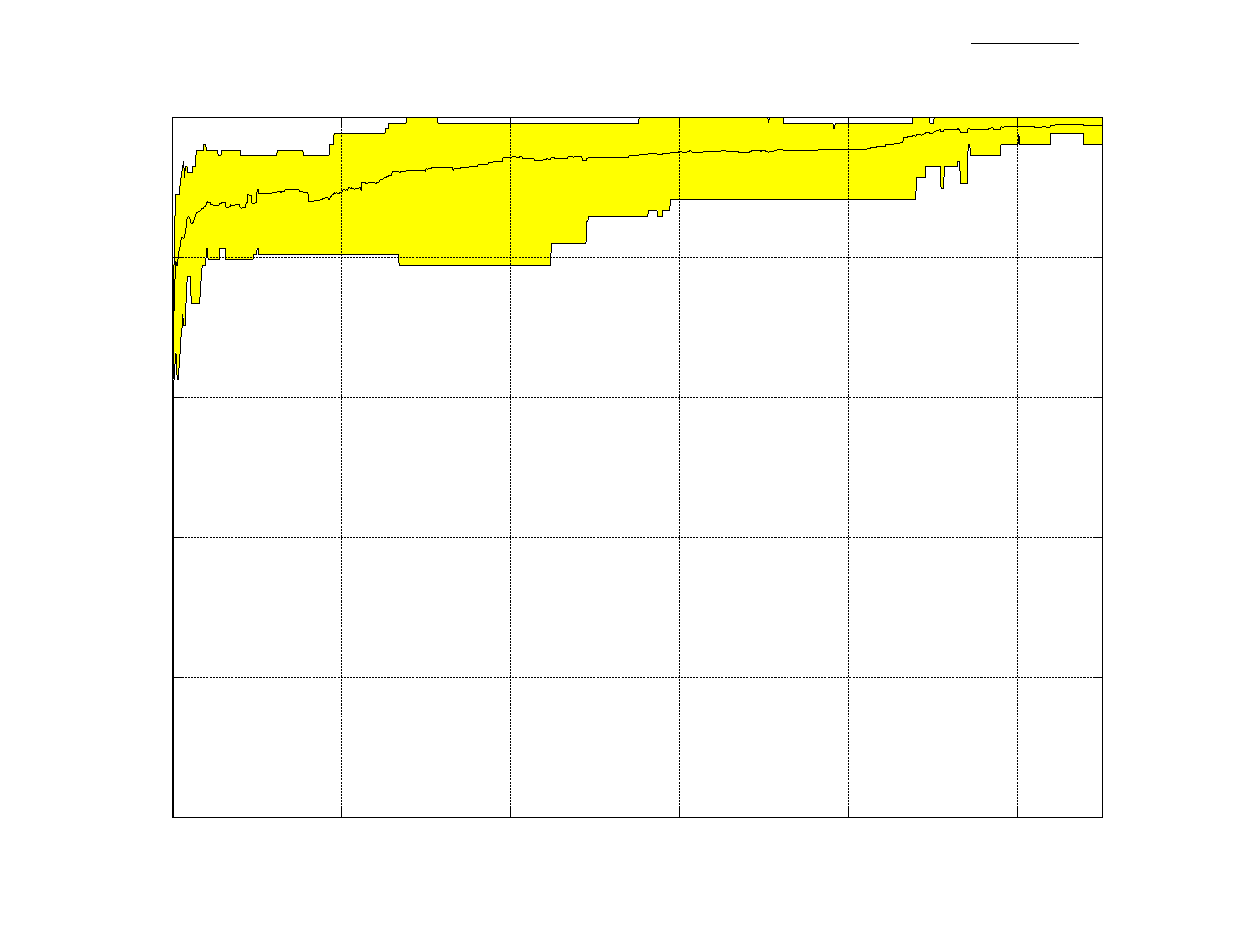
\includegraphics{./images/artificial/gmlaslcs0/positionGAex.eps}}%
    \gplfronttext
  \end{picture}%
\endgroup
}
  \put(-285,70){\rotatebox{90}{$Exact \: Match$}}
  \scalebox{0.8}{\put(-200,0){\rotatebox{0}{$iterations$}}}
  \label{fig:gmlaslcs0GAPosition7Ex}  
   
  \centering
  \scalebox{0.49}{\Large% GNUPLOT: LaTeX picture with Postscript
\begingroup
  \makeatletter
  \providecommand\color[2][]{%
    \GenericError{(gnuplot) \space\space\space\@spaces}{%
      Package color not loaded in conjunction with
      terminal option `colourtext'%
    }{See the gnuplot documentation for explanation.%
    }{Either use 'blacktext' in gnuplot or load the package
      color.sty in LaTeX.}%
    \renewcommand\color[2][]{}%
  }%
  \providecommand\includegraphics[2][]{%
    \GenericError{(gnuplot) \space\space\space\@spaces}{%
      Package graphicx or graphics not loaded%
    }{See the gnuplot documentation for explanation.%
    }{The gnuplot epslatex terminal needs graphicx.sty or graphics.sty.}%
    \renewcommand\includegraphics[2][]{}%
  }%
  \providecommand\rotatebox[2]{#2}%
  \@ifundefined{ifGPcolor}{%
    \newif\ifGPcolor
    \GPcolorfalse
  }{}%
  \@ifundefined{ifGPblacktext}{%
    \newif\ifGPblacktext
    \GPblacktexttrue
  }{}%
  % define a \g@addto@macro without @ in the name:
  \let\gplgaddtomacro\g@addto@macro
  % define empty templates for all commands taking text:
  \gdef\gplbacktext{}%
  \gdef\gplfronttext{}%
  \makeatother
  \ifGPblacktext
    % no textcolor at all
    \def\colorrgb#1{}%
    \def\colorgray#1{}%
  \else
    % gray or color?
    \ifGPcolor
      \def\colorrgb#1{\color[rgb]{#1}}%
      \def\colorgray#1{\color[gray]{#1}}%
      \expandafter\def\csname LTw\endcsname{\color{white}}%
      \expandafter\def\csname LTb\endcsname{\color{black}}%
      \expandafter\def\csname LTa\endcsname{\color{black}}%
      \expandafter\def\csname LT0\endcsname{\color[rgb]{1,0,0}}%
      \expandafter\def\csname LT1\endcsname{\color[rgb]{0,1,0}}%
      \expandafter\def\csname LT2\endcsname{\color[rgb]{0,0,1}}%
      \expandafter\def\csname LT3\endcsname{\color[rgb]{1,0,1}}%
      \expandafter\def\csname LT4\endcsname{\color[rgb]{0,1,1}}%
      \expandafter\def\csname LT5\endcsname{\color[rgb]{1,1,0}}%
      \expandafter\def\csname LT6\endcsname{\color[rgb]{0,0,0}}%
      \expandafter\def\csname LT7\endcsname{\color[rgb]{1,0.3,0}}%
      \expandafter\def\csname LT8\endcsname{\color[rgb]{0.5,0.5,0.5}}%
    \else
      % gray
      \def\colorrgb#1{\color{black}}%
      \def\colorgray#1{\color[gray]{#1}}%
      \expandafter\def\csname LTw\endcsname{\color{white}}%
      \expandafter\def\csname LTb\endcsname{\color{black}}%
      \expandafter\def\csname LTa\endcsname{\color{black}}%
      \expandafter\def\csname LT0\endcsname{\color{black}}%
      \expandafter\def\csname LT1\endcsname{\color{black}}%
      \expandafter\def\csname LT2\endcsname{\color{black}}%
      \expandafter\def\csname LT3\endcsname{\color{black}}%
      \expandafter\def\csname LT4\endcsname{\color{black}}%
      \expandafter\def\csname LT5\endcsname{\color{black}}%
      \expandafter\def\csname LT6\endcsname{\color{black}}%
      \expandafter\def\csname LT7\endcsname{\color{black}}%
      \expandafter\def\csname LT8\endcsname{\color{black}}%
    \fi
  \fi
  \setlength{\unitlength}{0.0500bp}%
  \begin{picture}(11520.00,8640.00)%
    \gplgaddtomacro\gplbacktext{%
    }%
    \gplgaddtomacro\gplfronttext{%
      \csname LTb\endcsname%
      \put(9049,8377){\makebox(0,0)[r]{\strut{}$GMl-ASLCS_{\:0GA} \: mean \: BAM \: coverage \: in \: mlPosition_7$}}%
      \colorrgb{0.00,0.00,0.00}%
      \put(1257,950){\makebox(0,0)[r]{\strut{}$0$}}%
      \colorrgb{0.00,0.00,0.00}%
      \put(1257,1910){\makebox(0,0)[r]{\strut{}$0.1$}}%
      \colorrgb{0.00,0.00,0.00}%
      \put(1257,2869){\makebox(0,0)[r]{\strut{}$0.2$}}%
      \colorrgb{0.00,0.00,0.00}%
      \put(1257,3829){\makebox(0,0)[r]{\strut{}$0.3$}}%
      \colorrgb{0.00,0.00,0.00}%
      \put(1257,4789){\makebox(0,0)[r]{\strut{}$0.4$}}%
      \colorrgb{0.00,0.00,0.00}%
      \put(1257,5749){\makebox(0,0)[r]{\strut{}$0.5$}}%
      \colorrgb{0.00,0.00,0.00}%
      \put(1257,6708){\makebox(0,0)[r]{\strut{}$0.6$}}%
      \colorrgb{0.00,0.00,0.00}%
      \put(1257,7668){\makebox(0,0)[r]{\strut{}$0.7$}}%
      \colorrgb{0.00,0.00,0.00}%
      \put(1497,550){\makebox(0,0){\strut{}$0$}}%
      \colorrgb{0.00,0.00,0.00}%
      \put(3120,550){\makebox(0,0){\strut{}$200$}}%
      \colorrgb{0.00,0.00,0.00}%
      \put(4743,550){\makebox(0,0){\strut{}$400$}}%
      \colorrgb{0.00,0.00,0.00}%
      \put(6366,550){\makebox(0,0){\strut{}$600$}}%
      \colorrgb{0.00,0.00,0.00}%
      \put(7989,550){\makebox(0,0){\strut{}$800$}}%
      \colorrgb{0.00,0.00,0.00}%
      \put(9612,550){\makebox(0,0){\strut{}$1000$}}%
    }%
    \gplbacktext
    \put(0,0){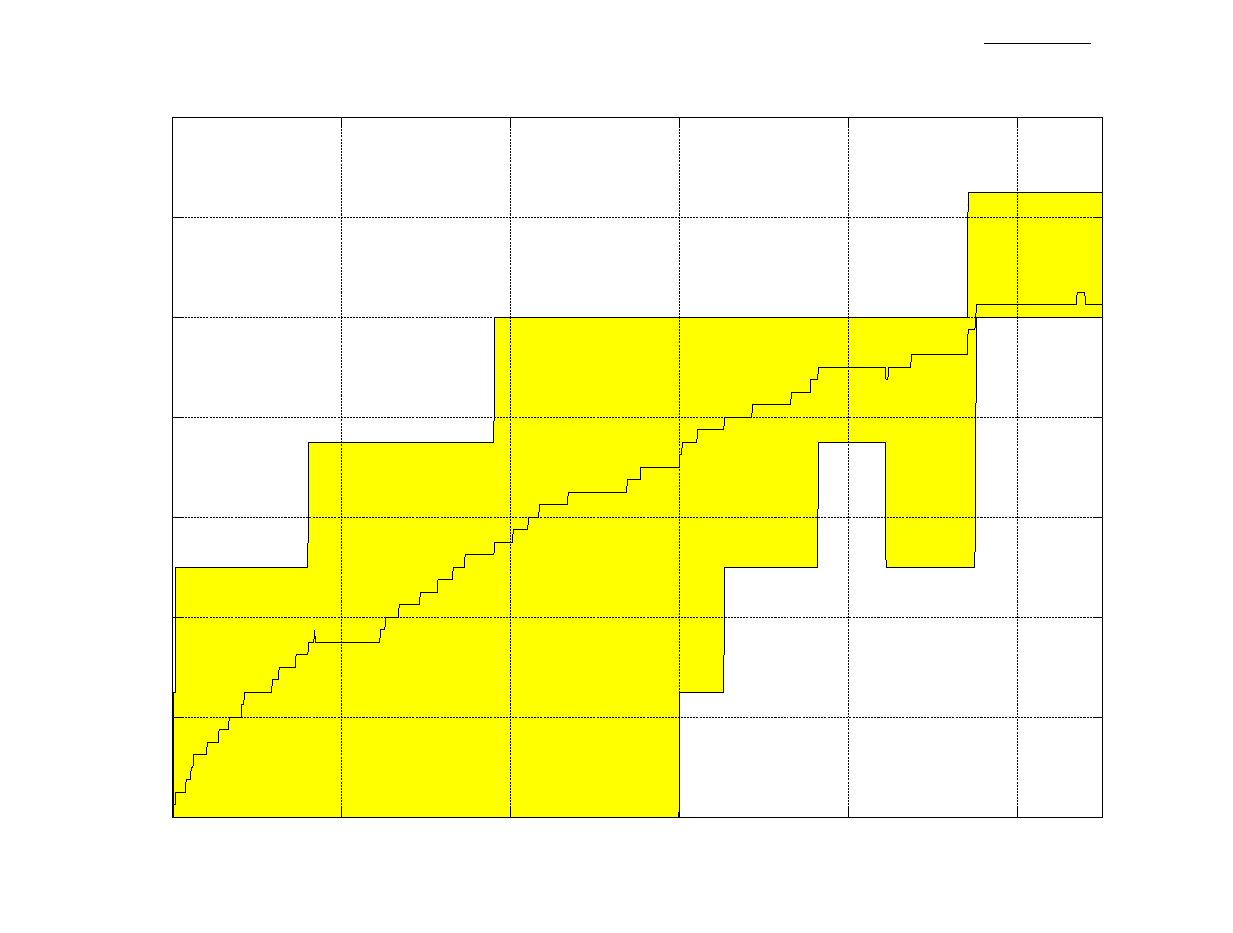
\includegraphics{./images/artificial/gmlaslcs0/positionGABAM.eps}}%
    \gplfronttext
  \end{picture}%
\endgroup
}
  \put(-285,80){\rotatebox{90}{$BAM$}}
  \scalebox{0.8}{\put(-200,0){\rotatebox{0}{$iterations$}}}
  \label{fig:gmlaslcs0GAPosition7BAM} 
\end{figure}

\begin{figure}[ht]
  \caption{Διαγράμματα χαρτογράφησης $mlPosition_{7}$ του GMl-ASLCS$_{\:0M}$.}
  \label{fig:gmlaslcs0MPosition7}
  \centering
  \scalebox{0.49}{\Large% GNUPLOT: LaTeX picture with Postscript
\begingroup
  \makeatletter
  \providecommand\color[2][]{%
    \GenericError{(gnuplot) \space\space\space\@spaces}{%
      Package color not loaded in conjunction with
      terminal option `colourtext'%
    }{See the gnuplot documentation for explanation.%
    }{Either use 'blacktext' in gnuplot or load the package
      color.sty in LaTeX.}%
    \renewcommand\color[2][]{}%
  }%
  \providecommand\includegraphics[2][]{%
    \GenericError{(gnuplot) \space\space\space\@spaces}{%
      Package graphicx or graphics not loaded%
    }{See the gnuplot documentation for explanation.%
    }{The gnuplot epslatex terminal needs graphicx.sty or graphics.sty.}%
    \renewcommand\includegraphics[2][]{}%
  }%
  \providecommand\rotatebox[2]{#2}%
  \@ifundefined{ifGPcolor}{%
    \newif\ifGPcolor
    \GPcolorfalse
  }{}%
  \@ifundefined{ifGPblacktext}{%
    \newif\ifGPblacktext
    \GPblacktexttrue
  }{}%
  % define a \g@addto@macro without @ in the name:
  \let\gplgaddtomacro\g@addto@macro
  % define empty templates for all commands taking text:
  \gdef\gplbacktext{}%
  \gdef\gplfronttext{}%
  \makeatother
  \ifGPblacktext
    % no textcolor at all
    \def\colorrgb#1{}%
    \def\colorgray#1{}%
  \else
    % gray or color?
    \ifGPcolor
      \def\colorrgb#1{\color[rgb]{#1}}%
      \def\colorgray#1{\color[gray]{#1}}%
      \expandafter\def\csname LTw\endcsname{\color{white}}%
      \expandafter\def\csname LTb\endcsname{\color{black}}%
      \expandafter\def\csname LTa\endcsname{\color{black}}%
      \expandafter\def\csname LT0\endcsname{\color[rgb]{1,0,0}}%
      \expandafter\def\csname LT1\endcsname{\color[rgb]{0,1,0}}%
      \expandafter\def\csname LT2\endcsname{\color[rgb]{0,0,1}}%
      \expandafter\def\csname LT3\endcsname{\color[rgb]{1,0,1}}%
      \expandafter\def\csname LT4\endcsname{\color[rgb]{0,1,1}}%
      \expandafter\def\csname LT5\endcsname{\color[rgb]{1,1,0}}%
      \expandafter\def\csname LT6\endcsname{\color[rgb]{0,0,0}}%
      \expandafter\def\csname LT7\endcsname{\color[rgb]{1,0.3,0}}%
      \expandafter\def\csname LT8\endcsname{\color[rgb]{0.5,0.5,0.5}}%
    \else
      % gray
      \def\colorrgb#1{\color{black}}%
      \def\colorgray#1{\color[gray]{#1}}%
      \expandafter\def\csname LTw\endcsname{\color{white}}%
      \expandafter\def\csname LTb\endcsname{\color{black}}%
      \expandafter\def\csname LTa\endcsname{\color{black}}%
      \expandafter\def\csname LT0\endcsname{\color{black}}%
      \expandafter\def\csname LT1\endcsname{\color{black}}%
      \expandafter\def\csname LT2\endcsname{\color{black}}%
      \expandafter\def\csname LT3\endcsname{\color{black}}%
      \expandafter\def\csname LT4\endcsname{\color{black}}%
      \expandafter\def\csname LT5\endcsname{\color{black}}%
      \expandafter\def\csname LT6\endcsname{\color{black}}%
      \expandafter\def\csname LT7\endcsname{\color{black}}%
      \expandafter\def\csname LT8\endcsname{\color{black}}%
    \fi
  \fi
  \setlength{\unitlength}{0.0500bp}%
  \begin{picture}(11520.00,8640.00)%
    \gplgaddtomacro\gplbacktext{%
    }%
    \gplgaddtomacro\gplfronttext{%
      \csname LTb\endcsname%
      \put(8569,8377){\makebox(0,0)[r]{\strut{}$GMl-ASLCS_{\:0M} \: mean \: accuracy \: in \: mlPosition_7$}}%
      \colorrgb{0.00,0.00,0.00}%
      \put(1257,950){\makebox(0,0)[r]{\strut{}$0$}}%
      \colorrgb{0.00,0.00,0.00}%
      \put(1257,2294){\makebox(0,0)[r]{\strut{}$0.2$}}%
      \colorrgb{0.00,0.00,0.00}%
      \put(1257,3637){\makebox(0,0)[r]{\strut{}$0.4$}}%
      \colorrgb{0.00,0.00,0.00}%
      \put(1257,4981){\makebox(0,0)[r]{\strut{}$0.6$}}%
      \colorrgb{0.00,0.00,0.00}%
      \put(1257,6324){\makebox(0,0)[r]{\strut{}$0.8$}}%
      \colorrgb{0.00,0.00,0.00}%
      \put(1257,7668){\makebox(0,0)[r]{\strut{}$1$}}%
      \colorrgb{0.00,0.00,0.00}%
      \put(1497,550){\makebox(0,0){\strut{}$0$}}%
      \colorrgb{0.00,0.00,0.00}%
      \put(3120,550){\makebox(0,0){\strut{}$200$}}%
      \colorrgb{0.00,0.00,0.00}%
      \put(4743,550){\makebox(0,0){\strut{}$400$}}%
      \colorrgb{0.00,0.00,0.00}%
      \put(6366,550){\makebox(0,0){\strut{}$600$}}%
      \colorrgb{0.00,0.00,0.00}%
      \put(7989,550){\makebox(0,0){\strut{}$800$}}%
      \colorrgb{0.00,0.00,0.00}%
      \put(9612,550){\makebox(0,0){\strut{}$1000$}}%
    }%
    \gplbacktext
    \put(0,0){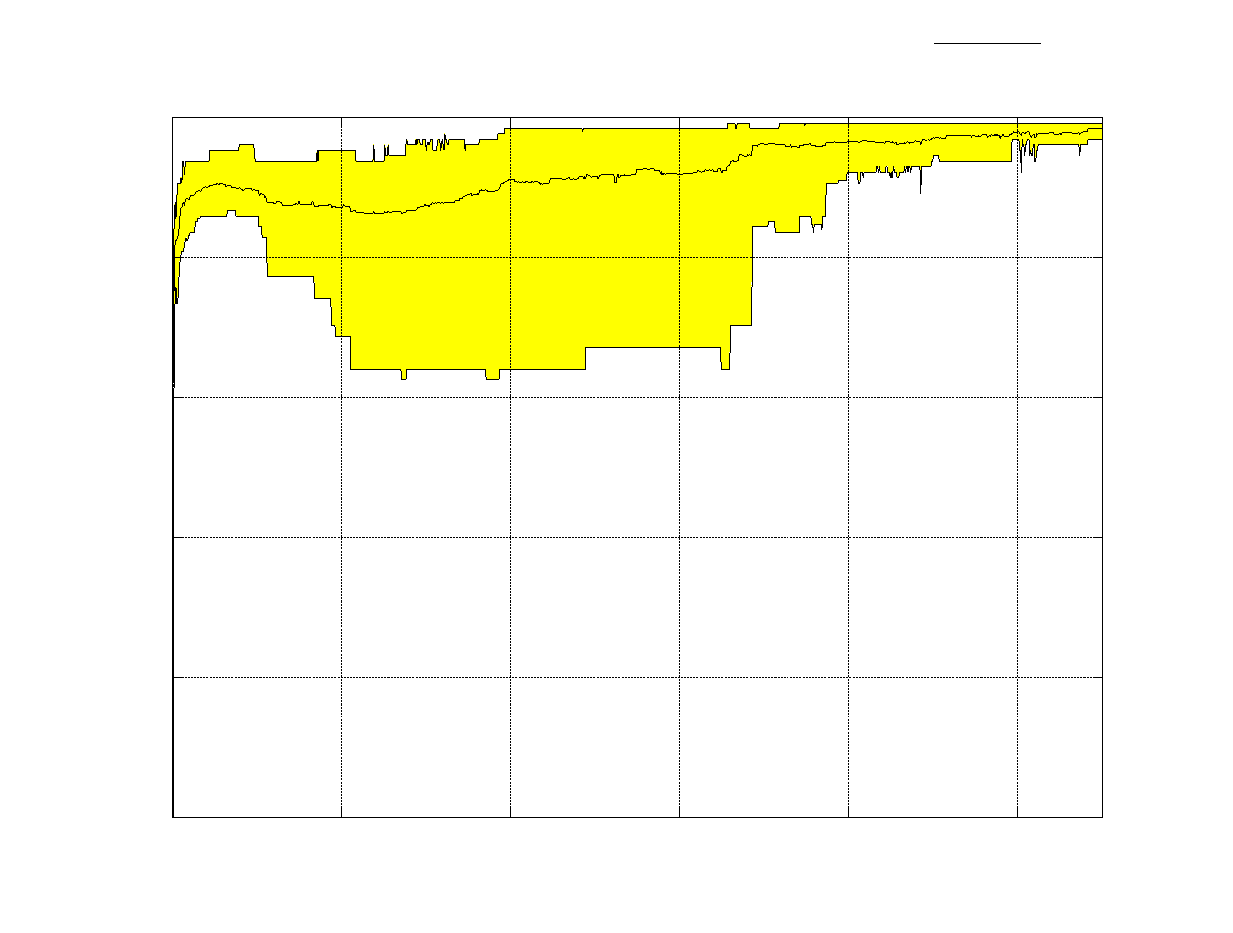
\includegraphics{./images/artificial/gmlaslcs0/positionMacc.eps}}%
    \gplfronttext
  \end{picture}%
\endgroup
}
  \put(-285,70){\rotatebox{90}{$Accuracy$}}
  \scalebox{0.8}{\put(-200,0){\rotatebox{0}{$iterations$}}}
  \label{fig:gmlaslcs0MPosition7Acc} 
  
  \centering
  \scalebox{0.49}{\Large% GNUPLOT: LaTeX picture with Postscript
\begingroup
  \makeatletter
  \providecommand\color[2][]{%
    \GenericError{(gnuplot) \space\space\space\@spaces}{%
      Package color not loaded in conjunction with
      terminal option `colourtext'%
    }{See the gnuplot documentation for explanation.%
    }{Either use 'blacktext' in gnuplot or load the package
      color.sty in LaTeX.}%
    \renewcommand\color[2][]{}%
  }%
  \providecommand\includegraphics[2][]{%
    \GenericError{(gnuplot) \space\space\space\@spaces}{%
      Package graphicx or graphics not loaded%
    }{See the gnuplot documentation for explanation.%
    }{The gnuplot epslatex terminal needs graphicx.sty or graphics.sty.}%
    \renewcommand\includegraphics[2][]{}%
  }%
  \providecommand\rotatebox[2]{#2}%
  \@ifundefined{ifGPcolor}{%
    \newif\ifGPcolor
    \GPcolorfalse
  }{}%
  \@ifundefined{ifGPblacktext}{%
    \newif\ifGPblacktext
    \GPblacktexttrue
  }{}%
  % define a \g@addto@macro without @ in the name:
  \let\gplgaddtomacro\g@addto@macro
  % define empty templates for all commands taking text:
  \gdef\gplbacktext{}%
  \gdef\gplfronttext{}%
  \makeatother
  \ifGPblacktext
    % no textcolor at all
    \def\colorrgb#1{}%
    \def\colorgray#1{}%
  \else
    % gray or color?
    \ifGPcolor
      \def\colorrgb#1{\color[rgb]{#1}}%
      \def\colorgray#1{\color[gray]{#1}}%
      \expandafter\def\csname LTw\endcsname{\color{white}}%
      \expandafter\def\csname LTb\endcsname{\color{black}}%
      \expandafter\def\csname LTa\endcsname{\color{black}}%
      \expandafter\def\csname LT0\endcsname{\color[rgb]{1,0,0}}%
      \expandafter\def\csname LT1\endcsname{\color[rgb]{0,1,0}}%
      \expandafter\def\csname LT2\endcsname{\color[rgb]{0,0,1}}%
      \expandafter\def\csname LT3\endcsname{\color[rgb]{1,0,1}}%
      \expandafter\def\csname LT4\endcsname{\color[rgb]{0,1,1}}%
      \expandafter\def\csname LT5\endcsname{\color[rgb]{1,1,0}}%
      \expandafter\def\csname LT6\endcsname{\color[rgb]{0,0,0}}%
      \expandafter\def\csname LT7\endcsname{\color[rgb]{1,0.3,0}}%
      \expandafter\def\csname LT8\endcsname{\color[rgb]{0.5,0.5,0.5}}%
    \else
      % gray
      \def\colorrgb#1{\color{black}}%
      \def\colorgray#1{\color[gray]{#1}}%
      \expandafter\def\csname LTw\endcsname{\color{white}}%
      \expandafter\def\csname LTb\endcsname{\color{black}}%
      \expandafter\def\csname LTa\endcsname{\color{black}}%
      \expandafter\def\csname LT0\endcsname{\color{black}}%
      \expandafter\def\csname LT1\endcsname{\color{black}}%
      \expandafter\def\csname LT2\endcsname{\color{black}}%
      \expandafter\def\csname LT3\endcsname{\color{black}}%
      \expandafter\def\csname LT4\endcsname{\color{black}}%
      \expandafter\def\csname LT5\endcsname{\color{black}}%
      \expandafter\def\csname LT6\endcsname{\color{black}}%
      \expandafter\def\csname LT7\endcsname{\color{black}}%
      \expandafter\def\csname LT8\endcsname{\color{black}}%
    \fi
  \fi
  \setlength{\unitlength}{0.0500bp}%
  \begin{picture}(11520.00,8640.00)%
    \gplgaddtomacro\gplbacktext{%
    }%
    \gplgaddtomacro\gplfronttext{%
      \csname LTb\endcsname%
      \put(8929,8377){\makebox(0,0)[r]{\strut{}$GMl-ASLCS_{\:0M} \: mean \: exact \: match \: in \: mlPosition_7$}}%
      \colorrgb{0.00,0.00,0.00}%
      \put(1257,950){\makebox(0,0)[r]{\strut{}$0$}}%
      \colorrgb{0.00,0.00,0.00}%
      \put(1257,2294){\makebox(0,0)[r]{\strut{}$0.2$}}%
      \colorrgb{0.00,0.00,0.00}%
      \put(1257,3637){\makebox(0,0)[r]{\strut{}$0.4$}}%
      \colorrgb{0.00,0.00,0.00}%
      \put(1257,4981){\makebox(0,0)[r]{\strut{}$0.6$}}%
      \colorrgb{0.00,0.00,0.00}%
      \put(1257,6324){\makebox(0,0)[r]{\strut{}$0.8$}}%
      \colorrgb{0.00,0.00,0.00}%
      \put(1257,7668){\makebox(0,0)[r]{\strut{}$1$}}%
      \colorrgb{0.00,0.00,0.00}%
      \put(1497,550){\makebox(0,0){\strut{}$0$}}%
      \colorrgb{0.00,0.00,0.00}%
      \put(3120,550){\makebox(0,0){\strut{}$200$}}%
      \colorrgb{0.00,0.00,0.00}%
      \put(4743,550){\makebox(0,0){\strut{}$400$}}%
      \colorrgb{0.00,0.00,0.00}%
      \put(6366,550){\makebox(0,0){\strut{}$600$}}%
      \colorrgb{0.00,0.00,0.00}%
      \put(7989,550){\makebox(0,0){\strut{}$800$}}%
      \colorrgb{0.00,0.00,0.00}%
      \put(9612,550){\makebox(0,0){\strut{}$1000$}}%
    }%
    \gplbacktext
    \put(0,0){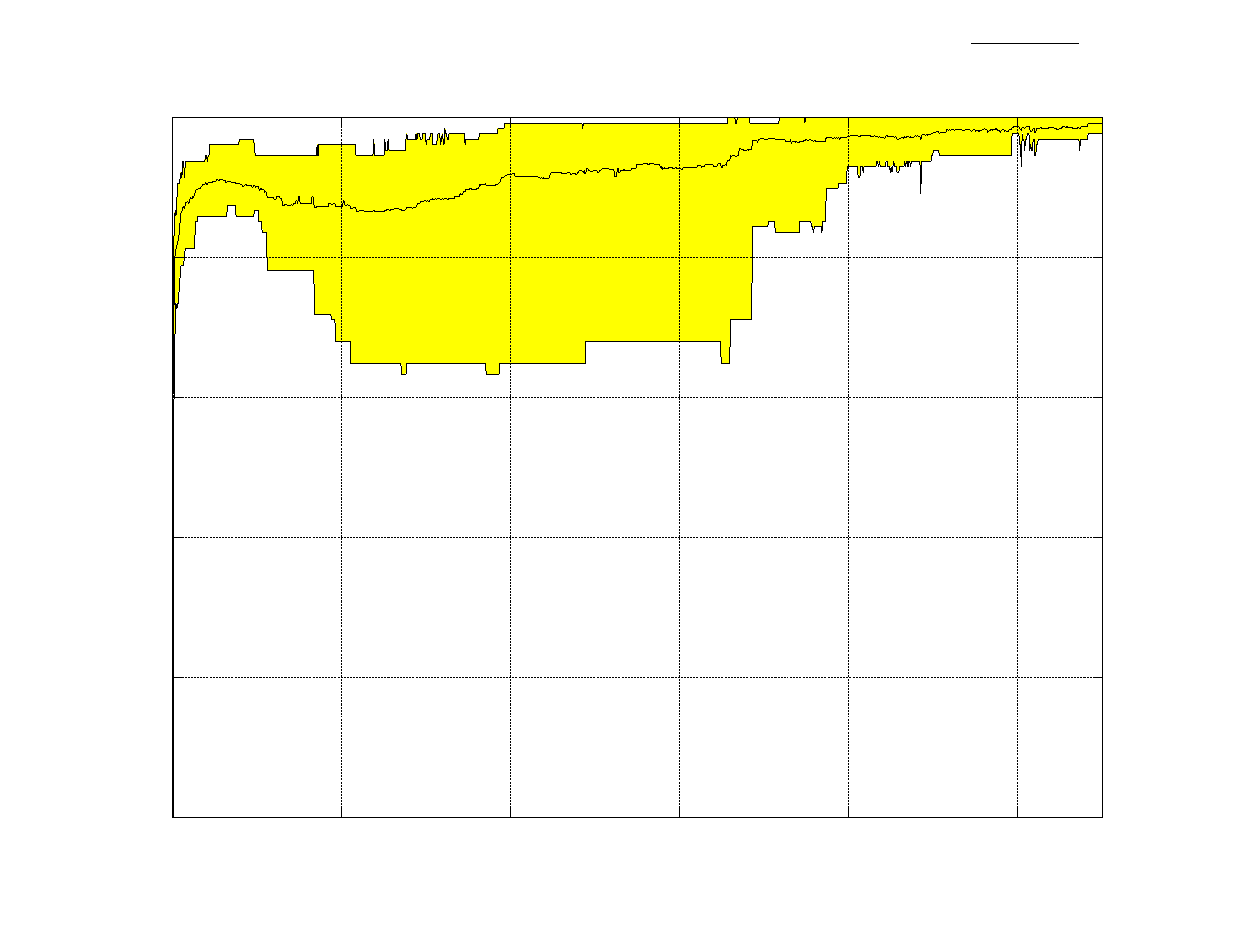
\includegraphics{./images/artificial/gmlaslcs0/positionMex.eps}}%
    \gplfronttext
  \end{picture}%
\endgroup
}
  \put(-285,70){\rotatebox{90}{$Exact \: Match$}}
  \scalebox{0.8}{\put(-200,0){\rotatebox{0}{$iterations$}}}
  \label{fig:gmlaslcs0MPosition7Ex}  
   
  \centering
  \scalebox{0.49}{\Large% GNUPLOT: LaTeX picture with Postscript
\begingroup
  \makeatletter
  \providecommand\color[2][]{%
    \GenericError{(gnuplot) \space\space\space\@spaces}{%
      Package color not loaded in conjunction with
      terminal option `colourtext'%
    }{See the gnuplot documentation for explanation.%
    }{Either use 'blacktext' in gnuplot or load the package
      color.sty in LaTeX.}%
    \renewcommand\color[2][]{}%
  }%
  \providecommand\includegraphics[2][]{%
    \GenericError{(gnuplot) \space\space\space\@spaces}{%
      Package graphicx or graphics not loaded%
    }{See the gnuplot documentation for explanation.%
    }{The gnuplot epslatex terminal needs graphicx.sty or graphics.sty.}%
    \renewcommand\includegraphics[2][]{}%
  }%
  \providecommand\rotatebox[2]{#2}%
  \@ifundefined{ifGPcolor}{%
    \newif\ifGPcolor
    \GPcolorfalse
  }{}%
  \@ifundefined{ifGPblacktext}{%
    \newif\ifGPblacktext
    \GPblacktexttrue
  }{}%
  % define a \g@addto@macro without @ in the name:
  \let\gplgaddtomacro\g@addto@macro
  % define empty templates for all commands taking text:
  \gdef\gplbacktext{}%
  \gdef\gplfronttext{}%
  \makeatother
  \ifGPblacktext
    % no textcolor at all
    \def\colorrgb#1{}%
    \def\colorgray#1{}%
  \else
    % gray or color?
    \ifGPcolor
      \def\colorrgb#1{\color[rgb]{#1}}%
      \def\colorgray#1{\color[gray]{#1}}%
      \expandafter\def\csname LTw\endcsname{\color{white}}%
      \expandafter\def\csname LTb\endcsname{\color{black}}%
      \expandafter\def\csname LTa\endcsname{\color{black}}%
      \expandafter\def\csname LT0\endcsname{\color[rgb]{1,0,0}}%
      \expandafter\def\csname LT1\endcsname{\color[rgb]{0,1,0}}%
      \expandafter\def\csname LT2\endcsname{\color[rgb]{0,0,1}}%
      \expandafter\def\csname LT3\endcsname{\color[rgb]{1,0,1}}%
      \expandafter\def\csname LT4\endcsname{\color[rgb]{0,1,1}}%
      \expandafter\def\csname LT5\endcsname{\color[rgb]{1,1,0}}%
      \expandafter\def\csname LT6\endcsname{\color[rgb]{0,0,0}}%
      \expandafter\def\csname LT7\endcsname{\color[rgb]{1,0.3,0}}%
      \expandafter\def\csname LT8\endcsname{\color[rgb]{0.5,0.5,0.5}}%
    \else
      % gray
      \def\colorrgb#1{\color{black}}%
      \def\colorgray#1{\color[gray]{#1}}%
      \expandafter\def\csname LTw\endcsname{\color{white}}%
      \expandafter\def\csname LTb\endcsname{\color{black}}%
      \expandafter\def\csname LTa\endcsname{\color{black}}%
      \expandafter\def\csname LT0\endcsname{\color{black}}%
      \expandafter\def\csname LT1\endcsname{\color{black}}%
      \expandafter\def\csname LT2\endcsname{\color{black}}%
      \expandafter\def\csname LT3\endcsname{\color{black}}%
      \expandafter\def\csname LT4\endcsname{\color{black}}%
      \expandafter\def\csname LT5\endcsname{\color{black}}%
      \expandafter\def\csname LT6\endcsname{\color{black}}%
      \expandafter\def\csname LT7\endcsname{\color{black}}%
      \expandafter\def\csname LT8\endcsname{\color{black}}%
    \fi
  \fi
  \setlength{\unitlength}{0.0500bp}%
  \begin{picture}(11520.00,8640.00)%
    \gplgaddtomacro\gplbacktext{%
    }%
    \gplgaddtomacro\gplfronttext{%
      \csname LTb\endcsname%
      \put(9049,8377){\makebox(0,0)[r]{\strut{}$GMl-ASLCS_{\:0M} \: mean \: BAM \: coverage \: in \: mlPosition_7$}}%
      \colorrgb{0.00,0.00,0.00}%
      \put(1257,950){\makebox(0,0)[r]{\strut{}$0$}}%
      \colorrgb{0.00,0.00,0.00}%
      \put(1257,1622){\makebox(0,0)[r]{\strut{}$0.05$}}%
      \colorrgb{0.00,0.00,0.00}%
      \put(1257,2294){\makebox(0,0)[r]{\strut{}$0.1$}}%
      \colorrgb{0.00,0.00,0.00}%
      \put(1257,2965){\makebox(0,0)[r]{\strut{}$0.15$}}%
      \colorrgb{0.00,0.00,0.00}%
      \put(1257,3637){\makebox(0,0)[r]{\strut{}$0.2$}}%
      \colorrgb{0.00,0.00,0.00}%
      \put(1257,4309){\makebox(0,0)[r]{\strut{}$0.25$}}%
      \colorrgb{0.00,0.00,0.00}%
      \put(1257,4981){\makebox(0,0)[r]{\strut{}$0.3$}}%
      \colorrgb{0.00,0.00,0.00}%
      \put(1257,5653){\makebox(0,0)[r]{\strut{}$0.35$}}%
      \colorrgb{0.00,0.00,0.00}%
      \put(1257,6324){\makebox(0,0)[r]{\strut{}$0.4$}}%
      \colorrgb{0.00,0.00,0.00}%
      \put(1257,6996){\makebox(0,0)[r]{\strut{}$0.45$}}%
      \colorrgb{0.00,0.00,0.00}%
      \put(1257,7668){\makebox(0,0)[r]{\strut{}$0.5$}}%
      \colorrgb{0.00,0.00,0.00}%
      \put(1497,550){\makebox(0,0){\strut{}$0$}}%
      \colorrgb{0.00,0.00,0.00}%
      \put(3120,550){\makebox(0,0){\strut{}$200$}}%
      \colorrgb{0.00,0.00,0.00}%
      \put(4743,550){\makebox(0,0){\strut{}$400$}}%
      \colorrgb{0.00,0.00,0.00}%
      \put(6366,550){\makebox(0,0){\strut{}$600$}}%
      \colorrgb{0.00,0.00,0.00}%
      \put(7989,550){\makebox(0,0){\strut{}$800$}}%
      \colorrgb{0.00,0.00,0.00}%
      \put(9612,550){\makebox(0,0){\strut{}$1000$}}%
    }%
    \gplbacktext
    \put(0,0){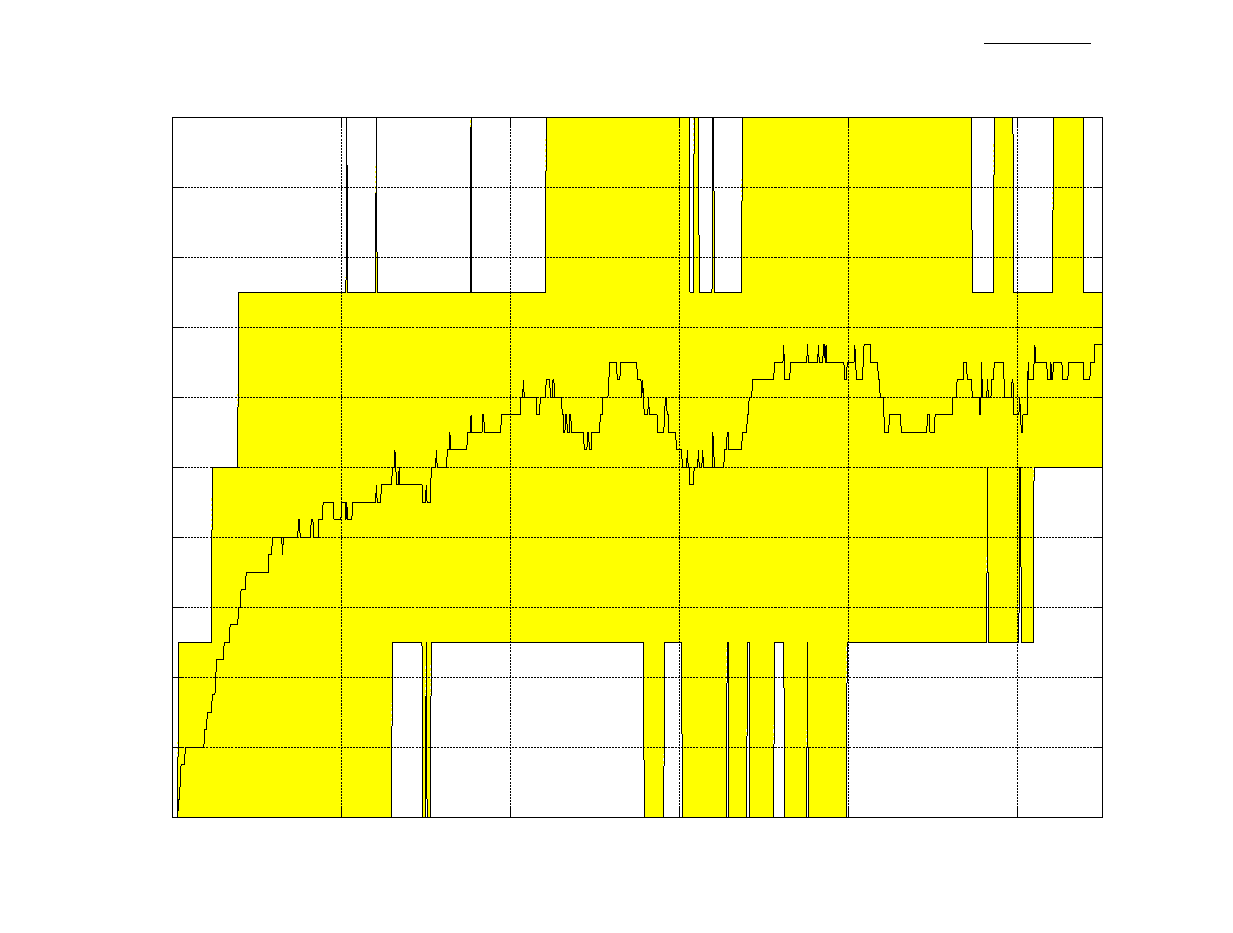
\includegraphics{./images/artificial/gmlaslcs0/positionMBAM.eps}}%
    \gplfronttext
  \end{picture}%
\endgroup
}
  \put(-285,80){\rotatebox{90}{$BAM$}}
  \scalebox{0.8}{\put(-200,0){\rotatebox{0}{$iterations$}}}
  \label{fig:gmlaslcs0MPosition7BAM} 
\end{figure}

\begin{figure}[ht]
  \caption{Διαγράμματα χαρτογράφησης $mlPosition_{7}$ του GMl-ASLCS$_{\:0C}$.}
  \label{fig:gmlaslcs0CPosition7}
  \centering
  \scalebox{0.49}{\Large% GNUPLOT: LaTeX picture with Postscript
\begingroup
  \makeatletter
  \providecommand\color[2][]{%
    \GenericError{(gnuplot) \space\space\space\@spaces}{%
      Package color not loaded in conjunction with
      terminal option `colourtext'%
    }{See the gnuplot documentation for explanation.%
    }{Either use 'blacktext' in gnuplot or load the package
      color.sty in LaTeX.}%
    \renewcommand\color[2][]{}%
  }%
  \providecommand\includegraphics[2][]{%
    \GenericError{(gnuplot) \space\space\space\@spaces}{%
      Package graphicx or graphics not loaded%
    }{See the gnuplot documentation for explanation.%
    }{The gnuplot epslatex terminal needs graphicx.sty or graphics.sty.}%
    \renewcommand\includegraphics[2][]{}%
  }%
  \providecommand\rotatebox[2]{#2}%
  \@ifundefined{ifGPcolor}{%
    \newif\ifGPcolor
    \GPcolorfalse
  }{}%
  \@ifundefined{ifGPblacktext}{%
    \newif\ifGPblacktext
    \GPblacktexttrue
  }{}%
  % define a \g@addto@macro without @ in the name:
  \let\gplgaddtomacro\g@addto@macro
  % define empty templates for all commands taking text:
  \gdef\gplbacktext{}%
  \gdef\gplfronttext{}%
  \makeatother
  \ifGPblacktext
    % no textcolor at all
    \def\colorrgb#1{}%
    \def\colorgray#1{}%
  \else
    % gray or color?
    \ifGPcolor
      \def\colorrgb#1{\color[rgb]{#1}}%
      \def\colorgray#1{\color[gray]{#1}}%
      \expandafter\def\csname LTw\endcsname{\color{white}}%
      \expandafter\def\csname LTb\endcsname{\color{black}}%
      \expandafter\def\csname LTa\endcsname{\color{black}}%
      \expandafter\def\csname LT0\endcsname{\color[rgb]{1,0,0}}%
      \expandafter\def\csname LT1\endcsname{\color[rgb]{0,1,0}}%
      \expandafter\def\csname LT2\endcsname{\color[rgb]{0,0,1}}%
      \expandafter\def\csname LT3\endcsname{\color[rgb]{1,0,1}}%
      \expandafter\def\csname LT4\endcsname{\color[rgb]{0,1,1}}%
      \expandafter\def\csname LT5\endcsname{\color[rgb]{1,1,0}}%
      \expandafter\def\csname LT6\endcsname{\color[rgb]{0,0,0}}%
      \expandafter\def\csname LT7\endcsname{\color[rgb]{1,0.3,0}}%
      \expandafter\def\csname LT8\endcsname{\color[rgb]{0.5,0.5,0.5}}%
    \else
      % gray
      \def\colorrgb#1{\color{black}}%
      \def\colorgray#1{\color[gray]{#1}}%
      \expandafter\def\csname LTw\endcsname{\color{white}}%
      \expandafter\def\csname LTb\endcsname{\color{black}}%
      \expandafter\def\csname LTa\endcsname{\color{black}}%
      \expandafter\def\csname LT0\endcsname{\color{black}}%
      \expandafter\def\csname LT1\endcsname{\color{black}}%
      \expandafter\def\csname LT2\endcsname{\color{black}}%
      \expandafter\def\csname LT3\endcsname{\color{black}}%
      \expandafter\def\csname LT4\endcsname{\color{black}}%
      \expandafter\def\csname LT5\endcsname{\color{black}}%
      \expandafter\def\csname LT6\endcsname{\color{black}}%
      \expandafter\def\csname LT7\endcsname{\color{black}}%
      \expandafter\def\csname LT8\endcsname{\color{black}}%
    \fi
  \fi
  \setlength{\unitlength}{0.0500bp}%
  \begin{picture}(11520.00,8640.00)%
    \gplgaddtomacro\gplbacktext{%
    }%
    \gplgaddtomacro\gplfronttext{%
      \csname LTb\endcsname%
      \put(8569,8377){\makebox(0,0)[r]{\strut{}$GMl-ASLCS_{\:0C} \: mean  \:accuracy  \:in  \:mlPosition_7$}}%
      \colorrgb{0.00,0.00,0.00}%
      \put(1257,950){\makebox(0,0)[r]{\strut{}$0$}}%
      \colorrgb{0.00,0.00,0.00}%
      \put(1257,2294){\makebox(0,0)[r]{\strut{}$0.2$}}%
      \colorrgb{0.00,0.00,0.00}%
      \put(1257,3637){\makebox(0,0)[r]{\strut{}$0.4$}}%
      \colorrgb{0.00,0.00,0.00}%
      \put(1257,4981){\makebox(0,0)[r]{\strut{}$0.6$}}%
      \colorrgb{0.00,0.00,0.00}%
      \put(1257,6324){\makebox(0,0)[r]{\strut{}$0.8$}}%
      \colorrgb{0.00,0.00,0.00}%
      \put(1257,7668){\makebox(0,0)[r]{\strut{}$1$}}%
      \colorrgb{0.00,0.00,0.00}%
      \put(1497,550){\makebox(0,0){\strut{}$0$}}%
      \colorrgb{0.00,0.00,0.00}%
      \put(3120,550){\makebox(0,0){\strut{}$200$}}%
      \colorrgb{0.00,0.00,0.00}%
      \put(4743,550){\makebox(0,0){\strut{}$400$}}%
      \colorrgb{0.00,0.00,0.00}%
      \put(6366,550){\makebox(0,0){\strut{}$600$}}%
      \colorrgb{0.00,0.00,0.00}%
      \put(7989,550){\makebox(0,0){\strut{}$800$}}%
      \colorrgb{0.00,0.00,0.00}%
      \put(9612,550){\makebox(0,0){\strut{}$1000$}}%
    }%
    \gplbacktext
    \put(0,0){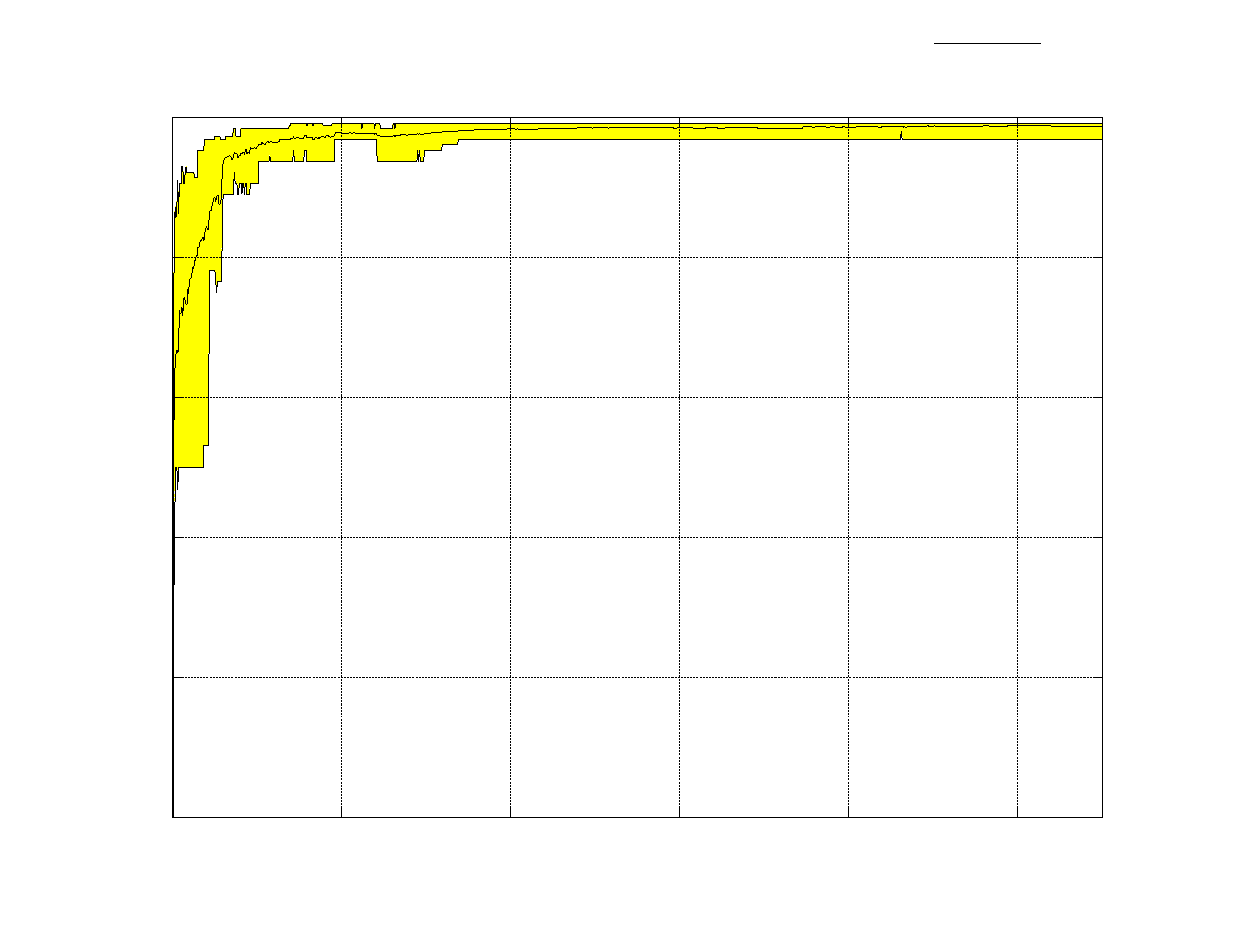
\includegraphics{./images/artificial/gmlaslcs0/positionCacc.eps}}%
    \gplfronttext
  \end{picture}%
\endgroup
}
  \put(-285,70){\rotatebox{90}{$Accuracy$}}
  \scalebox{0.8}{\put(-200,0){\rotatebox{0}{$iterations$}}}
  \label{fig:gmlaslcs0CPosition7Acc} 
  
  \centering
  \scalebox{0.49}{\Large% GNUPLOT: LaTeX picture with Postscript
\begingroup
  \makeatletter
  \providecommand\color[2][]{%
    \GenericError{(gnuplot) \space\space\space\@spaces}{%
      Package color not loaded in conjunction with
      terminal option `colourtext'%
    }{See the gnuplot documentation for explanation.%
    }{Either use 'blacktext' in gnuplot or load the package
      color.sty in LaTeX.}%
    \renewcommand\color[2][]{}%
  }%
  \providecommand\includegraphics[2][]{%
    \GenericError{(gnuplot) \space\space\space\@spaces}{%
      Package graphicx or graphics not loaded%
    }{See the gnuplot documentation for explanation.%
    }{The gnuplot epslatex terminal needs graphicx.sty or graphics.sty.}%
    \renewcommand\includegraphics[2][]{}%
  }%
  \providecommand\rotatebox[2]{#2}%
  \@ifundefined{ifGPcolor}{%
    \newif\ifGPcolor
    \GPcolorfalse
  }{}%
  \@ifundefined{ifGPblacktext}{%
    \newif\ifGPblacktext
    \GPblacktexttrue
  }{}%
  % define a \g@addto@macro without @ in the name:
  \let\gplgaddtomacro\g@addto@macro
  % define empty templates for all commands taking text:
  \gdef\gplbacktext{}%
  \gdef\gplfronttext{}%
  \makeatother
  \ifGPblacktext
    % no textcolor at all
    \def\colorrgb#1{}%
    \def\colorgray#1{}%
  \else
    % gray or color?
    \ifGPcolor
      \def\colorrgb#1{\color[rgb]{#1}}%
      \def\colorgray#1{\color[gray]{#1}}%
      \expandafter\def\csname LTw\endcsname{\color{white}}%
      \expandafter\def\csname LTb\endcsname{\color{black}}%
      \expandafter\def\csname LTa\endcsname{\color{black}}%
      \expandafter\def\csname LT0\endcsname{\color[rgb]{1,0,0}}%
      \expandafter\def\csname LT1\endcsname{\color[rgb]{0,1,0}}%
      \expandafter\def\csname LT2\endcsname{\color[rgb]{0,0,1}}%
      \expandafter\def\csname LT3\endcsname{\color[rgb]{1,0,1}}%
      \expandafter\def\csname LT4\endcsname{\color[rgb]{0,1,1}}%
      \expandafter\def\csname LT5\endcsname{\color[rgb]{1,1,0}}%
      \expandafter\def\csname LT6\endcsname{\color[rgb]{0,0,0}}%
      \expandafter\def\csname LT7\endcsname{\color[rgb]{1,0.3,0}}%
      \expandafter\def\csname LT8\endcsname{\color[rgb]{0.5,0.5,0.5}}%
    \else
      % gray
      \def\colorrgb#1{\color{black}}%
      \def\colorgray#1{\color[gray]{#1}}%
      \expandafter\def\csname LTw\endcsname{\color{white}}%
      \expandafter\def\csname LTb\endcsname{\color{black}}%
      \expandafter\def\csname LTa\endcsname{\color{black}}%
      \expandafter\def\csname LT0\endcsname{\color{black}}%
      \expandafter\def\csname LT1\endcsname{\color{black}}%
      \expandafter\def\csname LT2\endcsname{\color{black}}%
      \expandafter\def\csname LT3\endcsname{\color{black}}%
      \expandafter\def\csname LT4\endcsname{\color{black}}%
      \expandafter\def\csname LT5\endcsname{\color{black}}%
      \expandafter\def\csname LT6\endcsname{\color{black}}%
      \expandafter\def\csname LT7\endcsname{\color{black}}%
      \expandafter\def\csname LT8\endcsname{\color{black}}%
    \fi
  \fi
  \setlength{\unitlength}{0.0500bp}%
  \begin{picture}(11520.00,8640.00)%
    \gplgaddtomacro\gplbacktext{%
    }%
    \gplgaddtomacro\gplfronttext{%
      \csname LTb\endcsname%
      \put(8929,8377){\makebox(0,0)[r]{\strut{}$GMl-ASLCS_{\:0C} \: mean \: exact \: match \: in \: mlPosition_7$}}%
      \colorrgb{0.00,0.00,0.00}%
      \put(1257,950){\makebox(0,0)[r]{\strut{}$0$}}%
      \colorrgb{0.00,0.00,0.00}%
      \put(1257,2294){\makebox(0,0)[r]{\strut{}$0.2$}}%
      \colorrgb{0.00,0.00,0.00}%
      \put(1257,3637){\makebox(0,0)[r]{\strut{}$0.4$}}%
      \colorrgb{0.00,0.00,0.00}%
      \put(1257,4981){\makebox(0,0)[r]{\strut{}$0.6$}}%
      \colorrgb{0.00,0.00,0.00}%
      \put(1257,6324){\makebox(0,0)[r]{\strut{}$0.8$}}%
      \colorrgb{0.00,0.00,0.00}%
      \put(1257,7668){\makebox(0,0)[r]{\strut{}$1$}}%
      \colorrgb{0.00,0.00,0.00}%
      \put(1497,550){\makebox(0,0){\strut{}$0$}}%
      \colorrgb{0.00,0.00,0.00}%
      \put(3120,550){\makebox(0,0){\strut{}$200$}}%
      \colorrgb{0.00,0.00,0.00}%
      \put(4743,550){\makebox(0,0){\strut{}$400$}}%
      \colorrgb{0.00,0.00,0.00}%
      \put(6366,550){\makebox(0,0){\strut{}$600$}}%
      \colorrgb{0.00,0.00,0.00}%
      \put(7989,550){\makebox(0,0){\strut{}$800$}}%
      \colorrgb{0.00,0.00,0.00}%
      \put(9612,550){\makebox(0,0){\strut{}$1000$}}%
    }%
    \gplbacktext
    \put(0,0){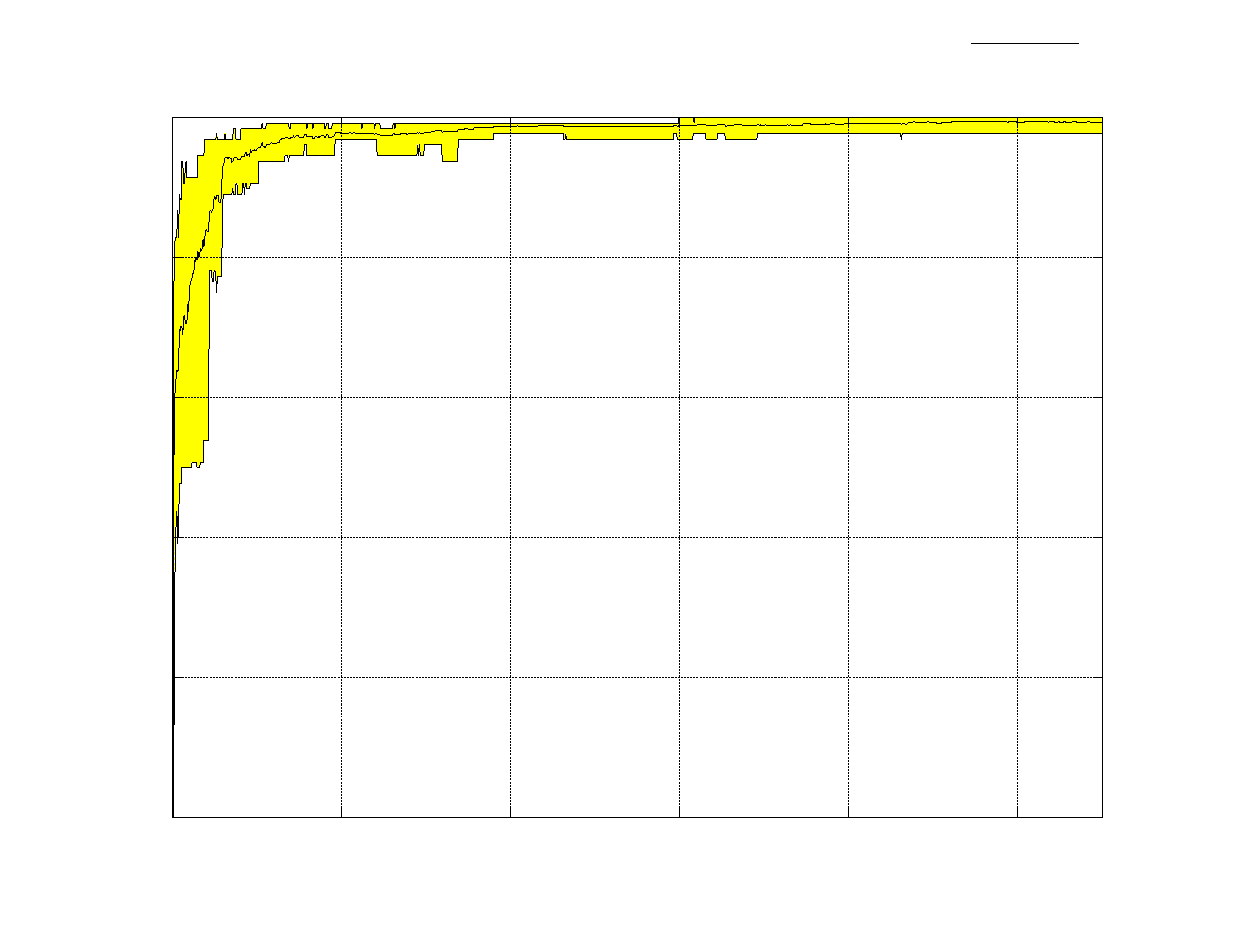
\includegraphics{./images/artificial/gmlaslcs0/positionCex.eps}}%
    \gplfronttext
  \end{picture}%
\endgroup
}
  \put(-285,70){\rotatebox{90}{$Exact \: Match$}}
  \scalebox{0.8}{\put(-200,0){\rotatebox{0}{$iterations$}}}
  \label{fig:gmlaslcs0CPosition7Ex}  
   
  \centering
  \scalebox{0.49}{\Large% GNUPLOT: LaTeX picture with Postscript
\begingroup
  \makeatletter
  \providecommand\color[2][]{%
    \GenericError{(gnuplot) \space\space\space\@spaces}{%
      Package color not loaded in conjunction with
      terminal option `colourtext'%
    }{See the gnuplot documentation for explanation.%
    }{Either use 'blacktext' in gnuplot or load the package
      color.sty in LaTeX.}%
    \renewcommand\color[2][]{}%
  }%
  \providecommand\includegraphics[2][]{%
    \GenericError{(gnuplot) \space\space\space\@spaces}{%
      Package graphicx or graphics not loaded%
    }{See the gnuplot documentation for explanation.%
    }{The gnuplot epslatex terminal needs graphicx.sty or graphics.sty.}%
    \renewcommand\includegraphics[2][]{}%
  }%
  \providecommand\rotatebox[2]{#2}%
  \@ifundefined{ifGPcolor}{%
    \newif\ifGPcolor
    \GPcolorfalse
  }{}%
  \@ifundefined{ifGPblacktext}{%
    \newif\ifGPblacktext
    \GPblacktexttrue
  }{}%
  % define a \g@addto@macro without @ in the name:
  \let\gplgaddtomacro\g@addto@macro
  % define empty templates for all commands taking text:
  \gdef\gplbacktext{}%
  \gdef\gplfronttext{}%
  \makeatother
  \ifGPblacktext
    % no textcolor at all
    \def\colorrgb#1{}%
    \def\colorgray#1{}%
  \else
    % gray or color?
    \ifGPcolor
      \def\colorrgb#1{\color[rgb]{#1}}%
      \def\colorgray#1{\color[gray]{#1}}%
      \expandafter\def\csname LTw\endcsname{\color{white}}%
      \expandafter\def\csname LTb\endcsname{\color{black}}%
      \expandafter\def\csname LTa\endcsname{\color{black}}%
      \expandafter\def\csname LT0\endcsname{\color[rgb]{1,0,0}}%
      \expandafter\def\csname LT1\endcsname{\color[rgb]{0,1,0}}%
      \expandafter\def\csname LT2\endcsname{\color[rgb]{0,0,1}}%
      \expandafter\def\csname LT3\endcsname{\color[rgb]{1,0,1}}%
      \expandafter\def\csname LT4\endcsname{\color[rgb]{0,1,1}}%
      \expandafter\def\csname LT5\endcsname{\color[rgb]{1,1,0}}%
      \expandafter\def\csname LT6\endcsname{\color[rgb]{0,0,0}}%
      \expandafter\def\csname LT7\endcsname{\color[rgb]{1,0.3,0}}%
      \expandafter\def\csname LT8\endcsname{\color[rgb]{0.5,0.5,0.5}}%
    \else
      % gray
      \def\colorrgb#1{\color{black}}%
      \def\colorgray#1{\color[gray]{#1}}%
      \expandafter\def\csname LTw\endcsname{\color{white}}%
      \expandafter\def\csname LTb\endcsname{\color{black}}%
      \expandafter\def\csname LTa\endcsname{\color{black}}%
      \expandafter\def\csname LT0\endcsname{\color{black}}%
      \expandafter\def\csname LT1\endcsname{\color{black}}%
      \expandafter\def\csname LT2\endcsname{\color{black}}%
      \expandafter\def\csname LT3\endcsname{\color{black}}%
      \expandafter\def\csname LT4\endcsname{\color{black}}%
      \expandafter\def\csname LT5\endcsname{\color{black}}%
      \expandafter\def\csname LT6\endcsname{\color{black}}%
      \expandafter\def\csname LT7\endcsname{\color{black}}%
      \expandafter\def\csname LT8\endcsname{\color{black}}%
    \fi
  \fi
  \setlength{\unitlength}{0.0500bp}%
  \begin{picture}(11520.00,8640.00)%
    \gplgaddtomacro\gplbacktext{%
    }%
    \gplgaddtomacro\gplfronttext{%
      \csname LTb\endcsname%
      \put(9049,8377){\makebox(0,0)[r]{\strut{}$GMl-ASLCS_{\:0C} \: mean \: BAM \: coverage \: in \: mlPosition_7$}}%
      \colorrgb{0.00,0.00,0.00}%
      \put(1257,950){\makebox(0,0)[r]{\strut{}$0$}}%
      \colorrgb{0.00,0.00,0.00}%
      \put(1257,2294){\makebox(0,0)[r]{\strut{}$0.2$}}%
      \colorrgb{0.00,0.00,0.00}%
      \put(1257,3637){\makebox(0,0)[r]{\strut{}$0.4$}}%
      \colorrgb{0.00,0.00,0.00}%
      \put(1257,4981){\makebox(0,0)[r]{\strut{}$0.6$}}%
      \colorrgb{0.00,0.00,0.00}%
      \put(1257,6324){\makebox(0,0)[r]{\strut{}$0.8$}}%
      \colorrgb{0.00,0.00,0.00}%
      \put(1257,7668){\makebox(0,0)[r]{\strut{}$1$}}%
      \colorrgb{0.00,0.00,0.00}%
      \put(1497,550){\makebox(0,0){\strut{}$0$}}%
      \colorrgb{0.00,0.00,0.00}%
      \put(3120,550){\makebox(0,0){\strut{}$200$}}%
      \colorrgb{0.00,0.00,0.00}%
      \put(4743,550){\makebox(0,0){\strut{}$400$}}%
      \colorrgb{0.00,0.00,0.00}%
      \put(6366,550){\makebox(0,0){\strut{}$600$}}%
      \colorrgb{0.00,0.00,0.00}%
      \put(7989,550){\makebox(0,0){\strut{}$800$}}%
      \colorrgb{0.00,0.00,0.00}%
      \put(9612,550){\makebox(0,0){\strut{}$1000$}}%
    }%
    \gplbacktext
    \put(0,0){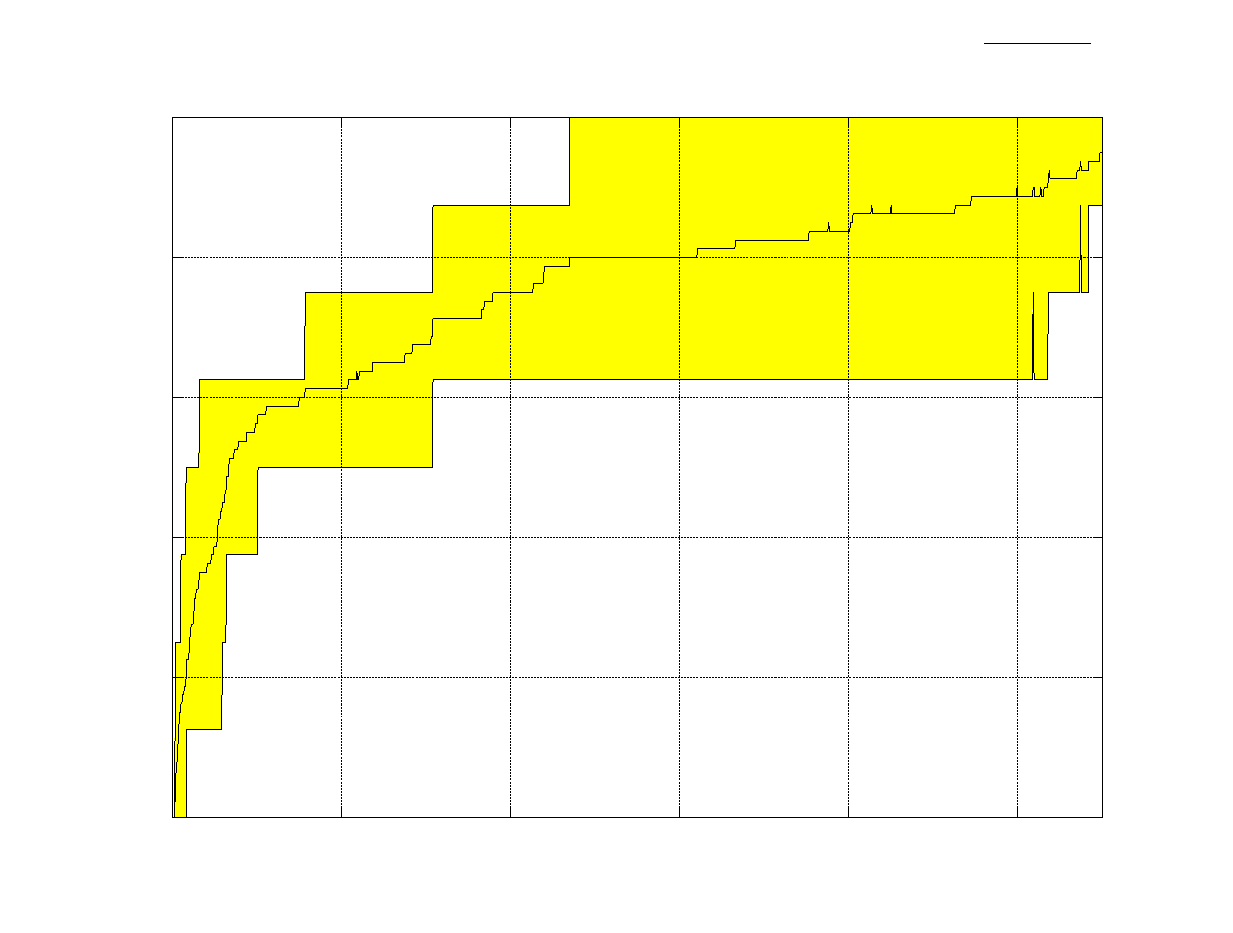
\includegraphics{./images/artificial/gmlaslcs0/positionCBAM.eps}}%
    \gplfronttext
  \end{picture}%
\endgroup
}
  \put(-285,80){\rotatebox{90}{$BAM$}}
  \scalebox{0.8}{\put(-200,0){\rotatebox{0}{$iterations$}}}
  \label{fig:gmlaslcs0CPosition7BAM} 
\end{figure}


Οι GMl-ASLCS$_{\:0D}$ και GMl-ASLCS$_{\:0GA}$, αν και δεν καταφέρνουν να επιτύχουν την πλήρη σύγκλιση τόσο στο ΧΒΑ, όσο και για τη μετρική της Ακρίβειας, επιπρόσθετα βελτιώνουν σε διαφορετικό βαθμό το ρυθμό και το χρόνο της σύγκλισης, σε σχέση με τον GMl-ASLCS$_{\:0}$, ενώ μειώνουν σε μικρό βαθμό το εύρος για τις μετρικές της Ακρίβειας, και σε μεγάλο, το εύρος ανάπτυξης του Βέλτιστου Χάρτη. Παρατηρούμε, δηλαδή μία βελτίωση ως προς την ικανότητα γενίκευσης, κάτι που απαιτείται από τη φύση του προβλήματος και της λύσης του, με ταυτόχρονη συγκράτηση της Ακρίβειας του τελικού μοντέλου. Λόγω της μικρής πολυκατηγορικής πυκνότητας του συνόλου $mlPosition_{7}$, η συμπεριφορά της Διασταύρωσης Δύο Τμημάτων προσεγγίζει αυτήν της Διασταύρωσης Ενός σημείου, καθώς δεν παρατηρούμε κάποια ραγδαία βελτίωση στο ρυθμό σύγκλισης του αλγορίθμου GMl-ASLCS$_{\:0GA}$.

Ο GMl-ASLCS$_{\:0M}$, παρ' όλη την ικανότητά του για γενίκευση, δε φαίνεται να μπορεί να αναπτύξει το σαφή βέλτιστο χάρτη του $mlPosition_{7}$ καλύτερα από τον GMl-ASLCS$_{\:0}$, και ακόμα χειρότερα δεν μπορεί να κρατήσει τους κανόνες που έχει βρει και που ανήκουν σε αυτόν, όπως φαίνεται από τις ταλαντώσεις της μέσης τιμής του ποσοστού εύρεσης του βέλτιστου χάρτη, αλλά και το εύρος των τιμών του. Ένα μέρος της ευθύνης, βέβαια, φέρει και το γεγονός ότι δεν τιμωρούνται οι κανόνες που φέρουν αδιαφορίες στο τμήμα της απόφασής τους, με αποτέλεσμα το σύστημα να μη μπορεί να διακρίνει αποτελεσματικά ανάμεσα σε έναν κανόνα του βέλτιστου χάρτη και έναν παρόμοιο, αλλά με αδιαφορίες στο τμήμα της απόφασής του, από τη στιγμή μάλιστα που ο βέλτιστος χάρτης περιλαμβάνει κανόνες από τους οποίους κανένας δεν αδιαφορεί για ετικέτες. Η ταλάντωση του μέσου όρου επίτευξης του βέλτιστου χάρτη και το γεγονός ότι στις τελευταίες επαναλήψεις ο αλγόριθμος αποκλίνει ελάχιστα από τις παραπάνω λύσεις, μάς κάνει να υποθέσουμε ότι η διαγραφή κανόνων από τα Match Sets, ως σχετικιστική λειτουργία, ίσως λειτουργεί αποσταθεροποιητικά για τους κανόνες που διατηρεί το σύστημα. Επομένως, μελλοντικά, θα έπρεπε να εξεταστεί η εφαρμογή ορίων καταλληλότητας για τη διαγραφή των κανόνων, ιδιαίτερα εάν δεν εφαρμόζεται έκπτωση της ακρίβειας για τους κανόνες με αδιαφορίες στις ετικέτες τους.

Τέλος, ο GMl-ASLCS$_{\:0C}$ καταφέρνει να συγκλίνει ταχύτερα από όλους τους τροποποιημένους GMl-ASLCS$_{\:0*}$ στο ανώφλι της Ακρίβειας και της Ακριβούς Ορθότητας για το πρόβλημα $mlPosition_{7}$. Η έκπτωση που επιφέρει στην καταλληλότητα των κανόνων με αδιαφορίες στις ετικέτες τους ($\phi=0.9$ αντί για $\phi=1$ για κάθε ετικέτα για την οποία αδιαφορεί ένας κανόνας), σε συνδυασμό με τη χαμηλή πολυκατηγορική πληθικότητα του συνόλου (εν προκειμένω την κατηγοριοποίηση των δειγμάτων το πολύ σε μία ετικέτα), και το γεγονός πως οι κανόνες του ΧΒΑ δεν περιλαμβάνουν αδιαφορίες στις αποφάσεις τους, βοηθάει το σύστημα να αναπτύξει κανόνες βέλτιστα γενικούς, με τη μέγιστη καταλληλότητα, αυξάνοντας και το ποσοστό εύρεσης των κανόνων του Βέλτιστου Χάρτη. Η αρνητική επίδραση του Γενετικού Αλγορίθμου με Διασταύρωση Ενός Σημείου φαίνεται ότι αποσβένεται λόγω της χαμηλής πολυκατηγορικής πληθικότητας και του γεγονότος ότι, πλέον, οι κανόνες που συμμετέχουν στα Correct Sets, από όπου επιλέγονται κανόνες προς αναπαραγωγή, διαθέτουν σε πολύ μικρότερο βαθμό αδιαφορίες στις ετικέτες τους σε σχέση με τον GMl-ASLCS$_{\:0}$. Συνεπώς, λόγω και της ανεξαρτησίας των ετικετών του συνόλου, οι αποφάσεις των κανόνων που συμμετέχουν στα διάφορα $[C]$ είναι σε μεγαλύτερο βαθμό ίδιες από ότι σε αυτά που σχηματίζονται στον GMl-ASLCS$_{\:0}$.









%-----------------------------------------identity-----------------------------------------%




\subsection{Οι τροποποιημένοι αλγόριθμοι GMl-ASLCS$_{\:0*}$ στο πρόβλημα $mlIdentity_{7}$}
Τα Σχήματα \ref{fig:gmlaslcs0Didentity7}, \ref{fig:gmlaslcs0GAidentity7}, \ref{fig:gmlaslcs0Midentity7} και \ref{fig:gmlaslcs0Cidentity7} παρουσιάζουν την εξέλιξη των μετρικών της Ακρίβειας, της Ακριβούς Ορθότητας και το ποσοστό κάλυψης του ΧBA για το σύνολο δεδομένων $mlIdentity_{7}$, των ΜαΣΤ GMl-ASLCS$_{\:0D}$, GMl-ASLCS$_{\:0GA}$, GMl-ASLCS$_{\:0M}$ και GMl-ASLCS$_{\:0C}$, αντίστοιχα.
\begin{figure}[ht]
  \caption{Διαγράμματα χαρτογράφησης $mlIdentity_{7}$ του GMl-ASLCS$_{\:0D}$.}
  \label{fig:gmlaslcs0Didentity7}
  \centering
  \scalebox{0.49}{\Large% GNUPLOT: LaTeX picture with Postscript
\begingroup
  \makeatletter
  \providecommand\color[2][]{%
    \GenericError{(gnuplot) \space\space\space\@spaces}{%
      Package color not loaded in conjunction with
      terminal option `colourtext'%
    }{See the gnuplot documentation for explanation.%
    }{Either use 'blacktext' in gnuplot or load the package
      color.sty in LaTeX.}%
    \renewcommand\color[2][]{}%
  }%
  \providecommand\includegraphics[2][]{%
    \GenericError{(gnuplot) \space\space\space\@spaces}{%
      Package graphicx or graphics not loaded%
    }{See the gnuplot documentation for explanation.%
    }{The gnuplot epslatex terminal needs graphicx.sty or graphics.sty.}%
    \renewcommand\includegraphics[2][]{}%
  }%
  \providecommand\rotatebox[2]{#2}%
  \@ifundefined{ifGPcolor}{%
    \newif\ifGPcolor
    \GPcolorfalse
  }{}%
  \@ifundefined{ifGPblacktext}{%
    \newif\ifGPblacktext
    \GPblacktexttrue
  }{}%
  % define a \g@addto@macro without @ in the name:
  \let\gplgaddtomacro\g@addto@macro
  % define empty templates for all commands taking text:
  \gdef\gplbacktext{}%
  \gdef\gplfronttext{}%
  \makeatother
  \ifGPblacktext
    % no textcolor at all
    \def\colorrgb#1{}%
    \def\colorgray#1{}%
  \else
    % gray or color?
    \ifGPcolor
      \def\colorrgb#1{\color[rgb]{#1}}%
      \def\colorgray#1{\color[gray]{#1}}%
      \expandafter\def\csname LTw\endcsname{\color{white}}%
      \expandafter\def\csname LTb\endcsname{\color{black}}%
      \expandafter\def\csname LTa\endcsname{\color{black}}%
      \expandafter\def\csname LT0\endcsname{\color[rgb]{1,0,0}}%
      \expandafter\def\csname LT1\endcsname{\color[rgb]{0,1,0}}%
      \expandafter\def\csname LT2\endcsname{\color[rgb]{0,0,1}}%
      \expandafter\def\csname LT3\endcsname{\color[rgb]{1,0,1}}%
      \expandafter\def\csname LT4\endcsname{\color[rgb]{0,1,1}}%
      \expandafter\def\csname LT5\endcsname{\color[rgb]{1,1,0}}%
      \expandafter\def\csname LT6\endcsname{\color[rgb]{0,0,0}}%
      \expandafter\def\csname LT7\endcsname{\color[rgb]{1,0.3,0}}%
      \expandafter\def\csname LT8\endcsname{\color[rgb]{0.5,0.5,0.5}}%
    \else
      % gray
      \def\colorrgb#1{\color{black}}%
      \def\colorgray#1{\color[gray]{#1}}%
      \expandafter\def\csname LTw\endcsname{\color{white}}%
      \expandafter\def\csname LTb\endcsname{\color{black}}%
      \expandafter\def\csname LTa\endcsname{\color{black}}%
      \expandafter\def\csname LT0\endcsname{\color{black}}%
      \expandafter\def\csname LT1\endcsname{\color{black}}%
      \expandafter\def\csname LT2\endcsname{\color{black}}%
      \expandafter\def\csname LT3\endcsname{\color{black}}%
      \expandafter\def\csname LT4\endcsname{\color{black}}%
      \expandafter\def\csname LT5\endcsname{\color{black}}%
      \expandafter\def\csname LT6\endcsname{\color{black}}%
      \expandafter\def\csname LT7\endcsname{\color{black}}%
      \expandafter\def\csname LT8\endcsname{\color{black}}%
    \fi
  \fi
  \setlength{\unitlength}{0.0500bp}%
  \begin{picture}(11520.00,8640.00)%
    \gplgaddtomacro\gplbacktext{%
    }%
    \gplgaddtomacro\gplfronttext{%
      \csname LTb\endcsname%
      \put(8569,8377){\makebox(0,0)[r]{\strut{}$GMl-ASLCS_{\:0D} \: mean  \:accuracy  \:in  \:mlIdentity_7$}}%
      \colorrgb{0.00,0.00,0.00}%
      \put(1257,950){\makebox(0,0)[r]{\strut{}$0$}}%
      \colorrgb{0.00,0.00,0.00}%
      \put(1257,2294){\makebox(0,0)[r]{\strut{}$0.2$}}%
      \colorrgb{0.00,0.00,0.00}%
      \put(1257,3637){\makebox(0,0)[r]{\strut{}$0.4$}}%
      \colorrgb{0.00,0.00,0.00}%
      \put(1257,4981){\makebox(0,0)[r]{\strut{}$0.6$}}%
      \colorrgb{0.00,0.00,0.00}%
      \put(1257,6324){\makebox(0,0)[r]{\strut{}$0.8$}}%
      \colorrgb{0.00,0.00,0.00}%
      \put(1257,7668){\makebox(0,0)[r]{\strut{}$1$}}%
      \colorrgb{0.00,0.00,0.00}%
      \put(1497,550){\makebox(0,0){\strut{}$0$}}%
      \colorrgb{0.00,0.00,0.00}%
      \put(3120,550){\makebox(0,0){\strut{}$200$}}%
      \colorrgb{0.00,0.00,0.00}%
      \put(4743,550){\makebox(0,0){\strut{}$400$}}%
      \colorrgb{0.00,0.00,0.00}%
      \put(6366,550){\makebox(0,0){\strut{}$600$}}%
      \colorrgb{0.00,0.00,0.00}%
      \put(7989,550){\makebox(0,0){\strut{}$800$}}%
      \colorrgb{0.00,0.00,0.00}%
      \put(9612,550){\makebox(0,0){\strut{}$1000$}}%
    }%
    \gplbacktext
    \put(0,0){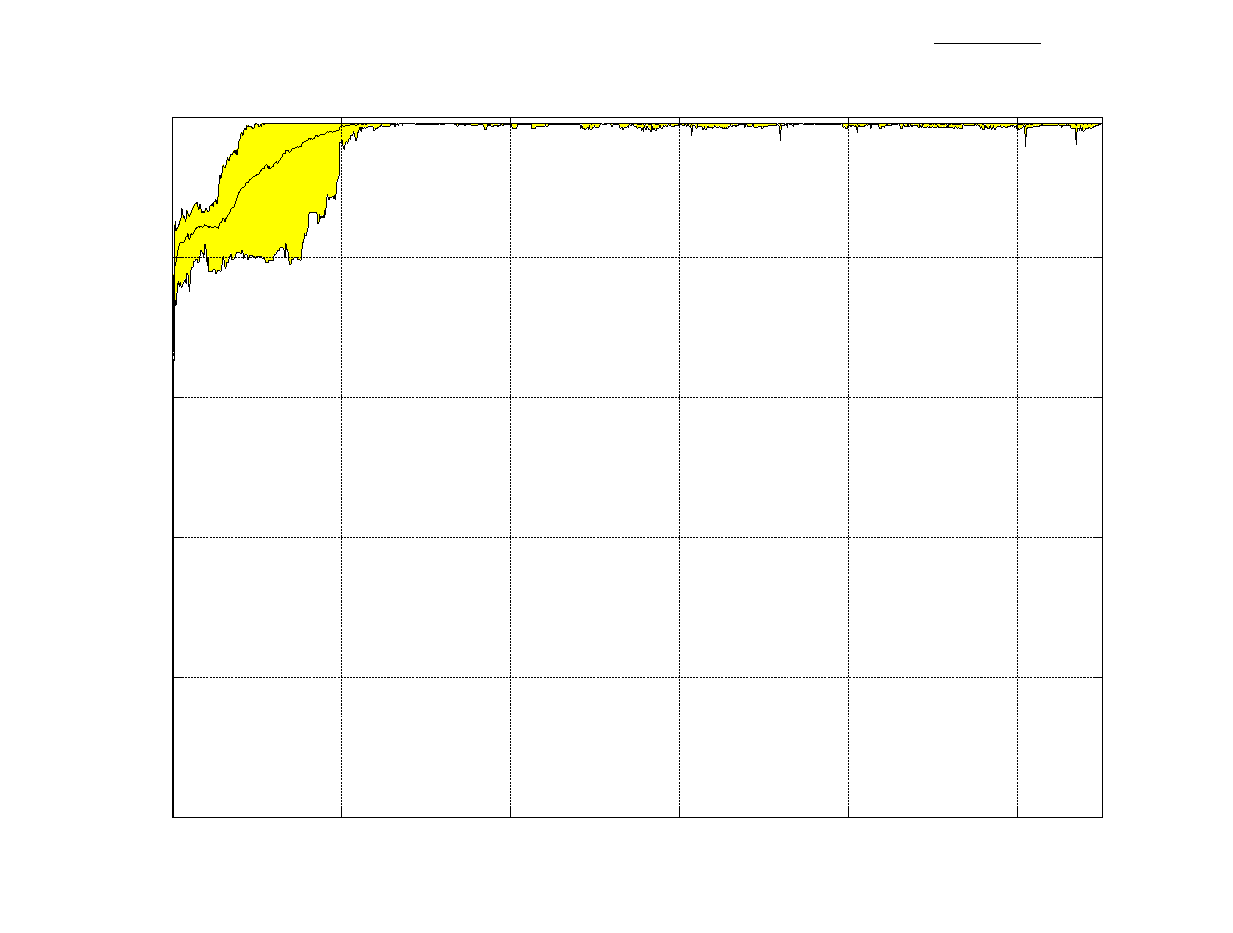
\includegraphics{./images/artificial/gmlaslcs0/identityDacc.eps}}%
    \gplfronttext
  \end{picture}%
\endgroup
}
  \put(-285,70){\rotatebox{90}{$Accuracy$}}
  \scalebox{0.8}{\put(-200,0){\rotatebox{0}{$iterations$}}}
  \label{fig:gmlaslcs0Didentity7Acc} 
  
  \centering
  \scalebox{0.49}{\Large% GNUPLOT: LaTeX picture with Postscript
\begingroup
  \makeatletter
  \providecommand\color[2][]{%
    \GenericError{(gnuplot) \space\space\space\@spaces}{%
      Package color not loaded in conjunction with
      terminal option `colourtext'%
    }{See the gnuplot documentation for explanation.%
    }{Either use 'blacktext' in gnuplot or load the package
      color.sty in LaTeX.}%
    \renewcommand\color[2][]{}%
  }%
  \providecommand\includegraphics[2][]{%
    \GenericError{(gnuplot) \space\space\space\@spaces}{%
      Package graphicx or graphics not loaded%
    }{See the gnuplot documentation for explanation.%
    }{The gnuplot epslatex terminal needs graphicx.sty or graphics.sty.}%
    \renewcommand\includegraphics[2][]{}%
  }%
  \providecommand\rotatebox[2]{#2}%
  \@ifundefined{ifGPcolor}{%
    \newif\ifGPcolor
    \GPcolorfalse
  }{}%
  \@ifundefined{ifGPblacktext}{%
    \newif\ifGPblacktext
    \GPblacktexttrue
  }{}%
  % define a \g@addto@macro without @ in the name:
  \let\gplgaddtomacro\g@addto@macro
  % define empty templates for all commands taking text:
  \gdef\gplbacktext{}%
  \gdef\gplfronttext{}%
  \makeatother
  \ifGPblacktext
    % no textcolor at all
    \def\colorrgb#1{}%
    \def\colorgray#1{}%
  \else
    % gray or color?
    \ifGPcolor
      \def\colorrgb#1{\color[rgb]{#1}}%
      \def\colorgray#1{\color[gray]{#1}}%
      \expandafter\def\csname LTw\endcsname{\color{white}}%
      \expandafter\def\csname LTb\endcsname{\color{black}}%
      \expandafter\def\csname LTa\endcsname{\color{black}}%
      \expandafter\def\csname LT0\endcsname{\color[rgb]{1,0,0}}%
      \expandafter\def\csname LT1\endcsname{\color[rgb]{0,1,0}}%
      \expandafter\def\csname LT2\endcsname{\color[rgb]{0,0,1}}%
      \expandafter\def\csname LT3\endcsname{\color[rgb]{1,0,1}}%
      \expandafter\def\csname LT4\endcsname{\color[rgb]{0,1,1}}%
      \expandafter\def\csname LT5\endcsname{\color[rgb]{1,1,0}}%
      \expandafter\def\csname LT6\endcsname{\color[rgb]{0,0,0}}%
      \expandafter\def\csname LT7\endcsname{\color[rgb]{1,0.3,0}}%
      \expandafter\def\csname LT8\endcsname{\color[rgb]{0.5,0.5,0.5}}%
    \else
      % gray
      \def\colorrgb#1{\color{black}}%
      \def\colorgray#1{\color[gray]{#1}}%
      \expandafter\def\csname LTw\endcsname{\color{white}}%
      \expandafter\def\csname LTb\endcsname{\color{black}}%
      \expandafter\def\csname LTa\endcsname{\color{black}}%
      \expandafter\def\csname LT0\endcsname{\color{black}}%
      \expandafter\def\csname LT1\endcsname{\color{black}}%
      \expandafter\def\csname LT2\endcsname{\color{black}}%
      \expandafter\def\csname LT3\endcsname{\color{black}}%
      \expandafter\def\csname LT4\endcsname{\color{black}}%
      \expandafter\def\csname LT5\endcsname{\color{black}}%
      \expandafter\def\csname LT6\endcsname{\color{black}}%
      \expandafter\def\csname LT7\endcsname{\color{black}}%
      \expandafter\def\csname LT8\endcsname{\color{black}}%
    \fi
  \fi
  \setlength{\unitlength}{0.0500bp}%
  \begin{picture}(11520.00,8640.00)%
    \gplgaddtomacro\gplbacktext{%
    }%
    \gplgaddtomacro\gplfronttext{%
      \csname LTb\endcsname%
      \put(8929,8377){\makebox(0,0)[r]{\strut{}$GMl-ASLCS_{\:0D} \: mean  \:exact \: match  \:in \: mlIdentity_7$}}%
      \colorrgb{0.00,0.00,0.00}%
      \put(1257,950){\makebox(0,0)[r]{\strut{}$0$}}%
      \colorrgb{0.00,0.00,0.00}%
      \put(1257,2294){\makebox(0,0)[r]{\strut{}$0.2$}}%
      \colorrgb{0.00,0.00,0.00}%
      \put(1257,3637){\makebox(0,0)[r]{\strut{}$0.4$}}%
      \colorrgb{0.00,0.00,0.00}%
      \put(1257,4981){\makebox(0,0)[r]{\strut{}$0.6$}}%
      \colorrgb{0.00,0.00,0.00}%
      \put(1257,6324){\makebox(0,0)[r]{\strut{}$0.8$}}%
      \colorrgb{0.00,0.00,0.00}%
      \put(1257,7668){\makebox(0,0)[r]{\strut{}$1$}}%
      \colorrgb{0.00,0.00,0.00}%
      \put(1497,550){\makebox(0,0){\strut{}$0$}}%
      \colorrgb{0.00,0.00,0.00}%
      \put(3120,550){\makebox(0,0){\strut{}$200$}}%
      \colorrgb{0.00,0.00,0.00}%
      \put(4743,550){\makebox(0,0){\strut{}$400$}}%
      \colorrgb{0.00,0.00,0.00}%
      \put(6366,550){\makebox(0,0){\strut{}$600$}}%
      \colorrgb{0.00,0.00,0.00}%
      \put(7989,550){\makebox(0,0){\strut{}$800$}}%
      \colorrgb{0.00,0.00,0.00}%
      \put(9612,550){\makebox(0,0){\strut{}$1000$}}%
    }%
    \gplbacktext
    \put(0,0){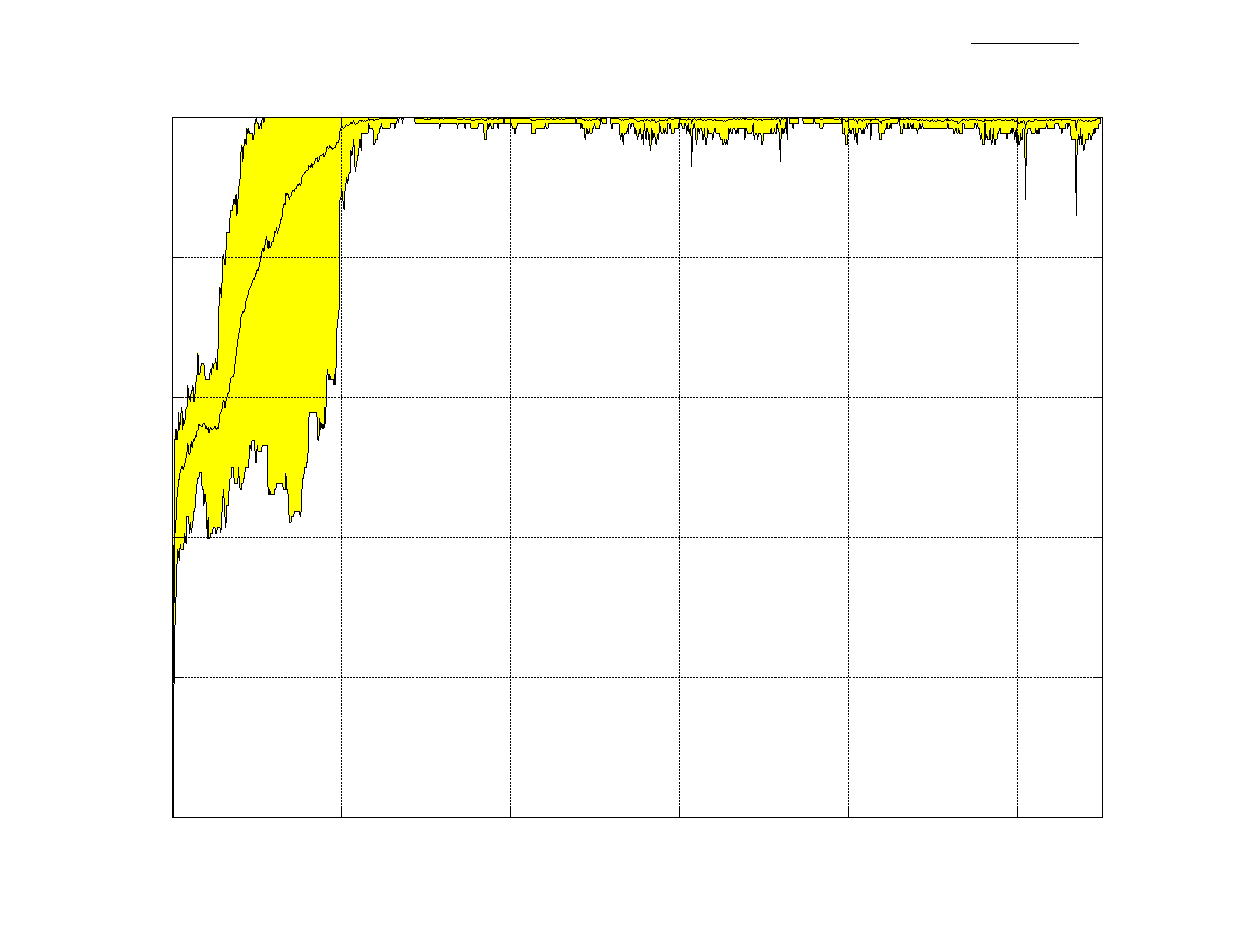
\includegraphics{./images/artificial/gmlaslcs0/identityDex.eps}}%
    \gplfronttext
  \end{picture}%
\endgroup
}
  \put(-285,70){\rotatebox{90}{$Exact \: Match$}}
  \scalebox{0.8}{\put(-200,0){\rotatebox{0}{$iterations$}}}
  \label{fig:gmlaslcs0Didentity7Ex}  
   
  \centering
  \scalebox{0.49}{\Large% GNUPLOT: LaTeX picture with Postscript
\begingroup
  \makeatletter
  \providecommand\color[2][]{%
    \GenericError{(gnuplot) \space\space\space\@spaces}{%
      Package color not loaded in conjunction with
      terminal option `colourtext'%
    }{See the gnuplot documentation for explanation.%
    }{Either use 'blacktext' in gnuplot or load the package
      color.sty in LaTeX.}%
    \renewcommand\color[2][]{}%
  }%
  \providecommand\includegraphics[2][]{%
    \GenericError{(gnuplot) \space\space\space\@spaces}{%
      Package graphicx or graphics not loaded%
    }{See the gnuplot documentation for explanation.%
    }{The gnuplot epslatex terminal needs graphicx.sty or graphics.sty.}%
    \renewcommand\includegraphics[2][]{}%
  }%
  \providecommand\rotatebox[2]{#2}%
  \@ifundefined{ifGPcolor}{%
    \newif\ifGPcolor
    \GPcolorfalse
  }{}%
  \@ifundefined{ifGPblacktext}{%
    \newif\ifGPblacktext
    \GPblacktexttrue
  }{}%
  % define a \g@addto@macro without @ in the name:
  \let\gplgaddtomacro\g@addto@macro
  % define empty templates for all commands taking text:
  \gdef\gplbacktext{}%
  \gdef\gplfronttext{}%
  \makeatother
  \ifGPblacktext
    % no textcolor at all
    \def\colorrgb#1{}%
    \def\colorgray#1{}%
  \else
    % gray or color?
    \ifGPcolor
      \def\colorrgb#1{\color[rgb]{#1}}%
      \def\colorgray#1{\color[gray]{#1}}%
      \expandafter\def\csname LTw\endcsname{\color{white}}%
      \expandafter\def\csname LTb\endcsname{\color{black}}%
      \expandafter\def\csname LTa\endcsname{\color{black}}%
      \expandafter\def\csname LT0\endcsname{\color[rgb]{1,0,0}}%
      \expandafter\def\csname LT1\endcsname{\color[rgb]{0,1,0}}%
      \expandafter\def\csname LT2\endcsname{\color[rgb]{0,0,1}}%
      \expandafter\def\csname LT3\endcsname{\color[rgb]{1,0,1}}%
      \expandafter\def\csname LT4\endcsname{\color[rgb]{0,1,1}}%
      \expandafter\def\csname LT5\endcsname{\color[rgb]{1,1,0}}%
      \expandafter\def\csname LT6\endcsname{\color[rgb]{0,0,0}}%
      \expandafter\def\csname LT7\endcsname{\color[rgb]{1,0.3,0}}%
      \expandafter\def\csname LT8\endcsname{\color[rgb]{0.5,0.5,0.5}}%
    \else
      % gray
      \def\colorrgb#1{\color{black}}%
      \def\colorgray#1{\color[gray]{#1}}%
      \expandafter\def\csname LTw\endcsname{\color{white}}%
      \expandafter\def\csname LTb\endcsname{\color{black}}%
      \expandafter\def\csname LTa\endcsname{\color{black}}%
      \expandafter\def\csname LT0\endcsname{\color{black}}%
      \expandafter\def\csname LT1\endcsname{\color{black}}%
      \expandafter\def\csname LT2\endcsname{\color{black}}%
      \expandafter\def\csname LT3\endcsname{\color{black}}%
      \expandafter\def\csname LT4\endcsname{\color{black}}%
      \expandafter\def\csname LT5\endcsname{\color{black}}%
      \expandafter\def\csname LT6\endcsname{\color{black}}%
      \expandafter\def\csname LT7\endcsname{\color{black}}%
      \expandafter\def\csname LT8\endcsname{\color{black}}%
    \fi
  \fi
  \setlength{\unitlength}{0.0500bp}%
  \begin{picture}(11520.00,8640.00)%
    \gplgaddtomacro\gplbacktext{%
    }%
    \gplgaddtomacro\gplfronttext{%
      \csname LTb\endcsname%
      \put(9049,8377){\makebox(0,0)[r]{\strut{}$GMl-ASLCS_{\:0D} \: mean \: BAM \: coverage \: in \: mlIdentity_7$}}%
      \colorrgb{0.00,0.00,0.00}%
      \put(1257,950){\makebox(0,0)[r]{\strut{}$0$}}%
      \colorrgb{0.00,0.00,0.00}%
      \put(1257,1622){\makebox(0,0)[r]{\strut{}$0.05$}}%
      \colorrgb{0.00,0.00,0.00}%
      \put(1257,2294){\makebox(0,0)[r]{\strut{}$0.1$}}%
      \colorrgb{0.00,0.00,0.00}%
      \put(1257,2965){\makebox(0,0)[r]{\strut{}$0.15$}}%
      \colorrgb{0.00,0.00,0.00}%
      \put(1257,3637){\makebox(0,0)[r]{\strut{}$0.2$}}%
      \colorrgb{0.00,0.00,0.00}%
      \put(1257,4309){\makebox(0,0)[r]{\strut{}$0.25$}}%
      \colorrgb{0.00,0.00,0.00}%
      \put(1257,4981){\makebox(0,0)[r]{\strut{}$0.3$}}%
      \colorrgb{0.00,0.00,0.00}%
      \put(1257,5653){\makebox(0,0)[r]{\strut{}$0.35$}}%
      \colorrgb{0.00,0.00,0.00}%
      \put(1257,6324){\makebox(0,0)[r]{\strut{}$0.4$}}%
      \colorrgb{0.00,0.00,0.00}%
      \put(1257,6996){\makebox(0,0)[r]{\strut{}$0.45$}}%
      \colorrgb{0.00,0.00,0.00}%
      \put(1257,7668){\makebox(0,0)[r]{\strut{}$0.5$}}%
      \colorrgb{0.00,0.00,0.00}%
      \put(1497,550){\makebox(0,0){\strut{}$0$}}%
      \colorrgb{0.00,0.00,0.00}%
      \put(3120,550){\makebox(0,0){\strut{}$200$}}%
      \colorrgb{0.00,0.00,0.00}%
      \put(4743,550){\makebox(0,0){\strut{}$400$}}%
      \colorrgb{0.00,0.00,0.00}%
      \put(6366,550){\makebox(0,0){\strut{}$600$}}%
      \colorrgb{0.00,0.00,0.00}%
      \put(7989,550){\makebox(0,0){\strut{}$800$}}%
      \colorrgb{0.00,0.00,0.00}%
      \put(9612,550){\makebox(0,0){\strut{}$1000$}}%
    }%
    \gplbacktext
    \put(0,0){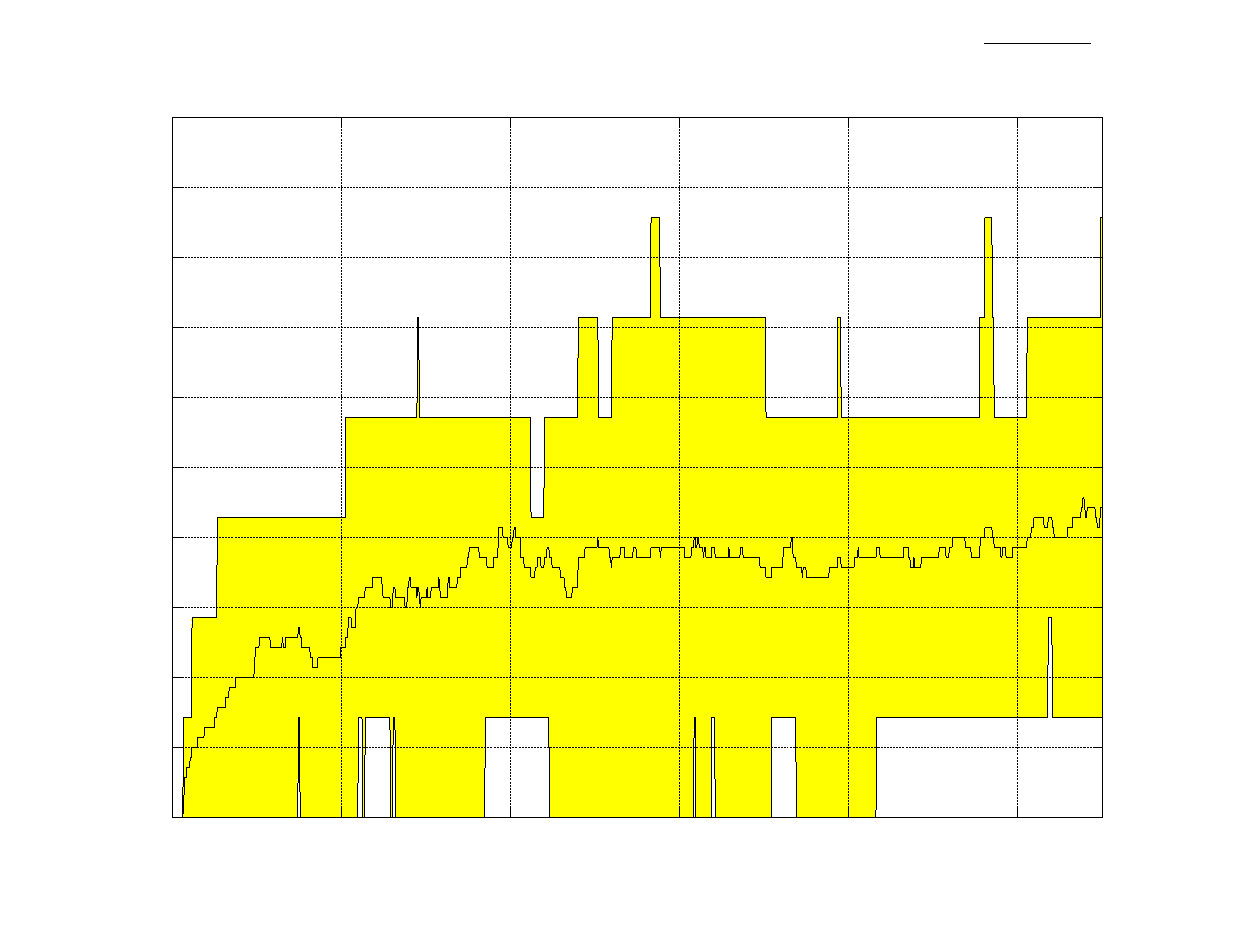
\includegraphics{./images/artificial/gmlaslcs0/identityDBAM.eps}}%
    \gplfronttext
  \end{picture}%
\endgroup
}
  \put(-285,80){\rotatebox{90}{$BAM$}}
  \scalebox{0.8}{\put(-200,0){\rotatebox{0}{$iterations$}}}
  \label{fig:gmlaslcs0Didentity7BAM} 
\end{figure}

\begin{figure}[ht]
  \caption{Διαγράμματα χαρτογράφησης $mlIdentity_{7}$ του GMl-ASLCS$_{\:0GA}$.}
  \label{fig:gmlaslcs0GAidentity7}
  \centering
  \scalebox{0.49}{\Large% GNUPLOT: LaTeX picture with Postscript
\begingroup
  \makeatletter
  \providecommand\color[2][]{%
    \GenericError{(gnuplot) \space\space\space\@spaces}{%
      Package color not loaded in conjunction with
      terminal option `colourtext'%
    }{See the gnuplot documentation for explanation.%
    }{Either use 'blacktext' in gnuplot or load the package
      color.sty in LaTeX.}%
    \renewcommand\color[2][]{}%
  }%
  \providecommand\includegraphics[2][]{%
    \GenericError{(gnuplot) \space\space\space\@spaces}{%
      Package graphicx or graphics not loaded%
    }{See the gnuplot documentation for explanation.%
    }{The gnuplot epslatex terminal needs graphicx.sty or graphics.sty.}%
    \renewcommand\includegraphics[2][]{}%
  }%
  \providecommand\rotatebox[2]{#2}%
  \@ifundefined{ifGPcolor}{%
    \newif\ifGPcolor
    \GPcolorfalse
  }{}%
  \@ifundefined{ifGPblacktext}{%
    \newif\ifGPblacktext
    \GPblacktexttrue
  }{}%
  % define a \g@addto@macro without @ in the name:
  \let\gplgaddtomacro\g@addto@macro
  % define empty templates for all commands taking text:
  \gdef\gplbacktext{}%
  \gdef\gplfronttext{}%
  \makeatother
  \ifGPblacktext
    % no textcolor at all
    \def\colorrgb#1{}%
    \def\colorgray#1{}%
  \else
    % gray or color?
    \ifGPcolor
      \def\colorrgb#1{\color[rgb]{#1}}%
      \def\colorgray#1{\color[gray]{#1}}%
      \expandafter\def\csname LTw\endcsname{\color{white}}%
      \expandafter\def\csname LTb\endcsname{\color{black}}%
      \expandafter\def\csname LTa\endcsname{\color{black}}%
      \expandafter\def\csname LT0\endcsname{\color[rgb]{1,0,0}}%
      \expandafter\def\csname LT1\endcsname{\color[rgb]{0,1,0}}%
      \expandafter\def\csname LT2\endcsname{\color[rgb]{0,0,1}}%
      \expandafter\def\csname LT3\endcsname{\color[rgb]{1,0,1}}%
      \expandafter\def\csname LT4\endcsname{\color[rgb]{0,1,1}}%
      \expandafter\def\csname LT5\endcsname{\color[rgb]{1,1,0}}%
      \expandafter\def\csname LT6\endcsname{\color[rgb]{0,0,0}}%
      \expandafter\def\csname LT7\endcsname{\color[rgb]{1,0.3,0}}%
      \expandafter\def\csname LT8\endcsname{\color[rgb]{0.5,0.5,0.5}}%
    \else
      % gray
      \def\colorrgb#1{\color{black}}%
      \def\colorgray#1{\color[gray]{#1}}%
      \expandafter\def\csname LTw\endcsname{\color{white}}%
      \expandafter\def\csname LTb\endcsname{\color{black}}%
      \expandafter\def\csname LTa\endcsname{\color{black}}%
      \expandafter\def\csname LT0\endcsname{\color{black}}%
      \expandafter\def\csname LT1\endcsname{\color{black}}%
      \expandafter\def\csname LT2\endcsname{\color{black}}%
      \expandafter\def\csname LT3\endcsname{\color{black}}%
      \expandafter\def\csname LT4\endcsname{\color{black}}%
      \expandafter\def\csname LT5\endcsname{\color{black}}%
      \expandafter\def\csname LT6\endcsname{\color{black}}%
      \expandafter\def\csname LT7\endcsname{\color{black}}%
      \expandafter\def\csname LT8\endcsname{\color{black}}%
    \fi
  \fi
  \setlength{\unitlength}{0.0500bp}%
  \begin{picture}(11520.00,8640.00)%
    \gplgaddtomacro\gplbacktext{%
    }%
    \gplgaddtomacro\gplfronttext{%
      \csname LTb\endcsname%
      \put(8569,8377){\makebox(0,0)[r]{\strut{}$GMl-ASLCS_{\:0GA} \: mean \: accuracy \: in \: mlIdentity_7$}}%
      \colorrgb{0.00,0.00,0.00}%
      \put(1257,950){\makebox(0,0)[r]{\strut{}$0$}}%
      \colorrgb{0.00,0.00,0.00}%
      \put(1257,2294){\makebox(0,0)[r]{\strut{}$0.2$}}%
      \colorrgb{0.00,0.00,0.00}%
      \put(1257,3637){\makebox(0,0)[r]{\strut{}$0.4$}}%
      \colorrgb{0.00,0.00,0.00}%
      \put(1257,4981){\makebox(0,0)[r]{\strut{}$0.6$}}%
      \colorrgb{0.00,0.00,0.00}%
      \put(1257,6324){\makebox(0,0)[r]{\strut{}$0.8$}}%
      \colorrgb{0.00,0.00,0.00}%
      \put(1257,7668){\makebox(0,0)[r]{\strut{}$1$}}%
      \colorrgb{0.00,0.00,0.00}%
      \put(1497,550){\makebox(0,0){\strut{}$0$}}%
      \colorrgb{0.00,0.00,0.00}%
      \put(3120,550){\makebox(0,0){\strut{}$200$}}%
      \colorrgb{0.00,0.00,0.00}%
      \put(4743,550){\makebox(0,0){\strut{}$400$}}%
      \colorrgb{0.00,0.00,0.00}%
      \put(6366,550){\makebox(0,0){\strut{}$600$}}%
      \colorrgb{0.00,0.00,0.00}%
      \put(7989,550){\makebox(0,0){\strut{}$800$}}%
      \colorrgb{0.00,0.00,0.00}%
      \put(9612,550){\makebox(0,0){\strut{}$1000$}}%
    }%
    \gplbacktext
    \put(0,0){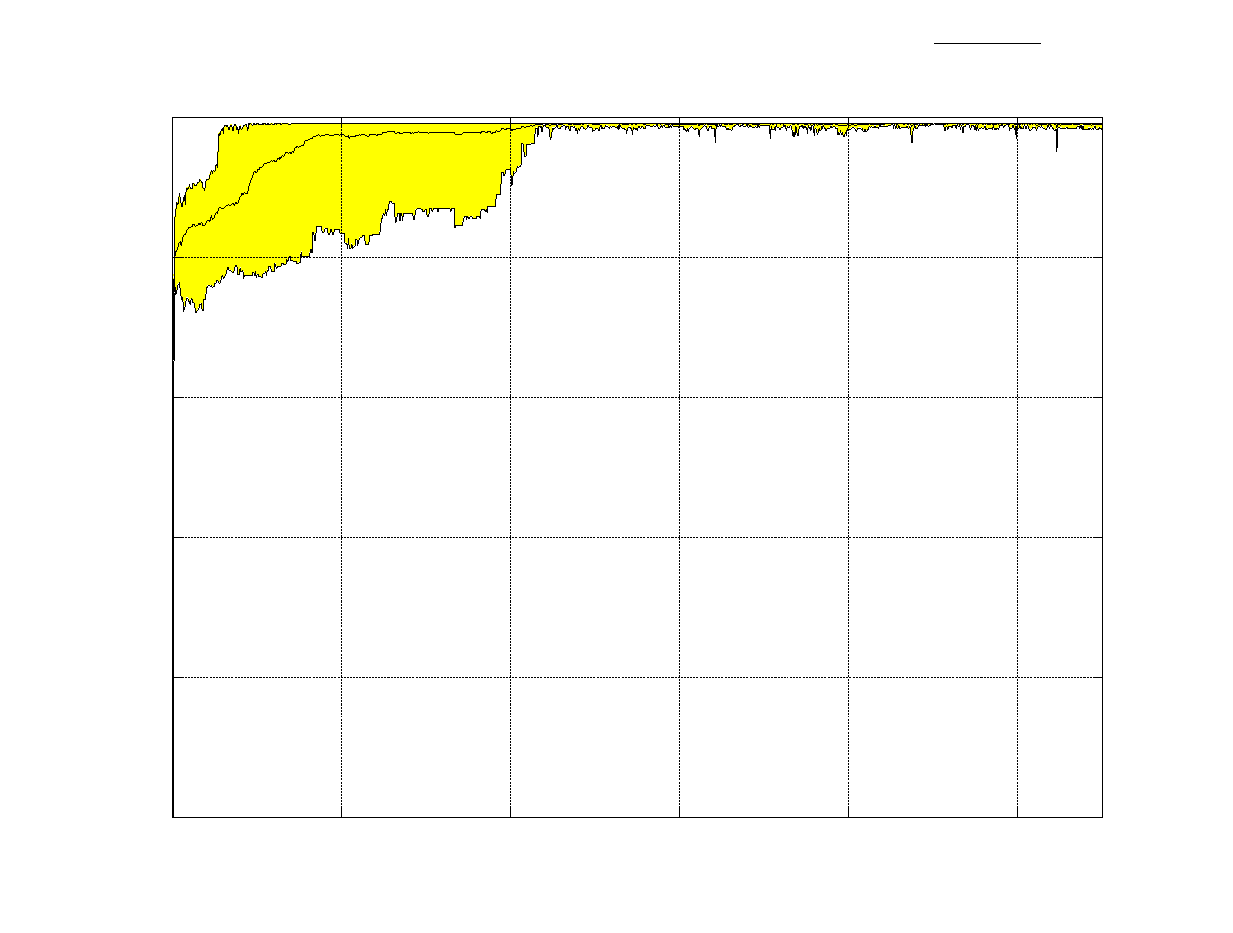
\includegraphics{./images/artificial/gmlaslcs0/identityGAacc.eps}}%
    \gplfronttext
  \end{picture}%
\endgroup
}
  \put(-285,70){\rotatebox{90}{$Accuracy$}}
  \scalebox{0.8}{\put(-200,0){\rotatebox{0}{$iterations$}}}
  \label{fig:gmlaslcs0GAidentity7Acc} 
  
  \centering
  \scalebox{0.49}{\Large% GNUPLOT: LaTeX picture with Postscript
\begingroup
  \makeatletter
  \providecommand\color[2][]{%
    \GenericError{(gnuplot) \space\space\space\@spaces}{%
      Package color not loaded in conjunction with
      terminal option `colourtext'%
    }{See the gnuplot documentation for explanation.%
    }{Either use 'blacktext' in gnuplot or load the package
      color.sty in LaTeX.}%
    \renewcommand\color[2][]{}%
  }%
  \providecommand\includegraphics[2][]{%
    \GenericError{(gnuplot) \space\space\space\@spaces}{%
      Package graphicx or graphics not loaded%
    }{See the gnuplot documentation for explanation.%
    }{The gnuplot epslatex terminal needs graphicx.sty or graphics.sty.}%
    \renewcommand\includegraphics[2][]{}%
  }%
  \providecommand\rotatebox[2]{#2}%
  \@ifundefined{ifGPcolor}{%
    \newif\ifGPcolor
    \GPcolorfalse
  }{}%
  \@ifundefined{ifGPblacktext}{%
    \newif\ifGPblacktext
    \GPblacktexttrue
  }{}%
  % define a \g@addto@macro without @ in the name:
  \let\gplgaddtomacro\g@addto@macro
  % define empty templates for all commands taking text:
  \gdef\gplbacktext{}%
  \gdef\gplfronttext{}%
  \makeatother
  \ifGPblacktext
    % no textcolor at all
    \def\colorrgb#1{}%
    \def\colorgray#1{}%
  \else
    % gray or color?
    \ifGPcolor
      \def\colorrgb#1{\color[rgb]{#1}}%
      \def\colorgray#1{\color[gray]{#1}}%
      \expandafter\def\csname LTw\endcsname{\color{white}}%
      \expandafter\def\csname LTb\endcsname{\color{black}}%
      \expandafter\def\csname LTa\endcsname{\color{black}}%
      \expandafter\def\csname LT0\endcsname{\color[rgb]{1,0,0}}%
      \expandafter\def\csname LT1\endcsname{\color[rgb]{0,1,0}}%
      \expandafter\def\csname LT2\endcsname{\color[rgb]{0,0,1}}%
      \expandafter\def\csname LT3\endcsname{\color[rgb]{1,0,1}}%
      \expandafter\def\csname LT4\endcsname{\color[rgb]{0,1,1}}%
      \expandafter\def\csname LT5\endcsname{\color[rgb]{1,1,0}}%
      \expandafter\def\csname LT6\endcsname{\color[rgb]{0,0,0}}%
      \expandafter\def\csname LT7\endcsname{\color[rgb]{1,0.3,0}}%
      \expandafter\def\csname LT8\endcsname{\color[rgb]{0.5,0.5,0.5}}%
    \else
      % gray
      \def\colorrgb#1{\color{black}}%
      \def\colorgray#1{\color[gray]{#1}}%
      \expandafter\def\csname LTw\endcsname{\color{white}}%
      \expandafter\def\csname LTb\endcsname{\color{black}}%
      \expandafter\def\csname LTa\endcsname{\color{black}}%
      \expandafter\def\csname LT0\endcsname{\color{black}}%
      \expandafter\def\csname LT1\endcsname{\color{black}}%
      \expandafter\def\csname LT2\endcsname{\color{black}}%
      \expandafter\def\csname LT3\endcsname{\color{black}}%
      \expandafter\def\csname LT4\endcsname{\color{black}}%
      \expandafter\def\csname LT5\endcsname{\color{black}}%
      \expandafter\def\csname LT6\endcsname{\color{black}}%
      \expandafter\def\csname LT7\endcsname{\color{black}}%
      \expandafter\def\csname LT8\endcsname{\color{black}}%
    \fi
  \fi
  \setlength{\unitlength}{0.0500bp}%
  \begin{picture}(11520.00,8640.00)%
    \gplgaddtomacro\gplbacktext{%
    }%
    \gplgaddtomacro\gplfronttext{%
      \csname LTb\endcsname%
      \put(8929,8377){\makebox(0,0)[r]{\strut{}$GMl-ASLCS_{\:0GA} \: mean \: exact \: match  \:in  \:mlIdentity_7$}}%
      \colorrgb{0.00,0.00,0.00}%
      \put(1257,950){\makebox(0,0)[r]{\strut{}$0$}}%
      \colorrgb{0.00,0.00,0.00}%
      \put(1257,2294){\makebox(0,0)[r]{\strut{}$0.2$}}%
      \colorrgb{0.00,0.00,0.00}%
      \put(1257,3637){\makebox(0,0)[r]{\strut{}$0.4$}}%
      \colorrgb{0.00,0.00,0.00}%
      \put(1257,4981){\makebox(0,0)[r]{\strut{}$0.6$}}%
      \colorrgb{0.00,0.00,0.00}%
      \put(1257,6324){\makebox(0,0)[r]{\strut{}$0.8$}}%
      \colorrgb{0.00,0.00,0.00}%
      \put(1257,7668){\makebox(0,0)[r]{\strut{}$1$}}%
      \colorrgb{0.00,0.00,0.00}%
      \put(1497,550){\makebox(0,0){\strut{}$0$}}%
      \colorrgb{0.00,0.00,0.00}%
      \put(3120,550){\makebox(0,0){\strut{}$200$}}%
      \colorrgb{0.00,0.00,0.00}%
      \put(4743,550){\makebox(0,0){\strut{}$400$}}%
      \colorrgb{0.00,0.00,0.00}%
      \put(6366,550){\makebox(0,0){\strut{}$600$}}%
      \colorrgb{0.00,0.00,0.00}%
      \put(7989,550){\makebox(0,0){\strut{}$800$}}%
      \colorrgb{0.00,0.00,0.00}%
      \put(9612,550){\makebox(0,0){\strut{}$1000$}}%
    }%
    \gplbacktext
    \put(0,0){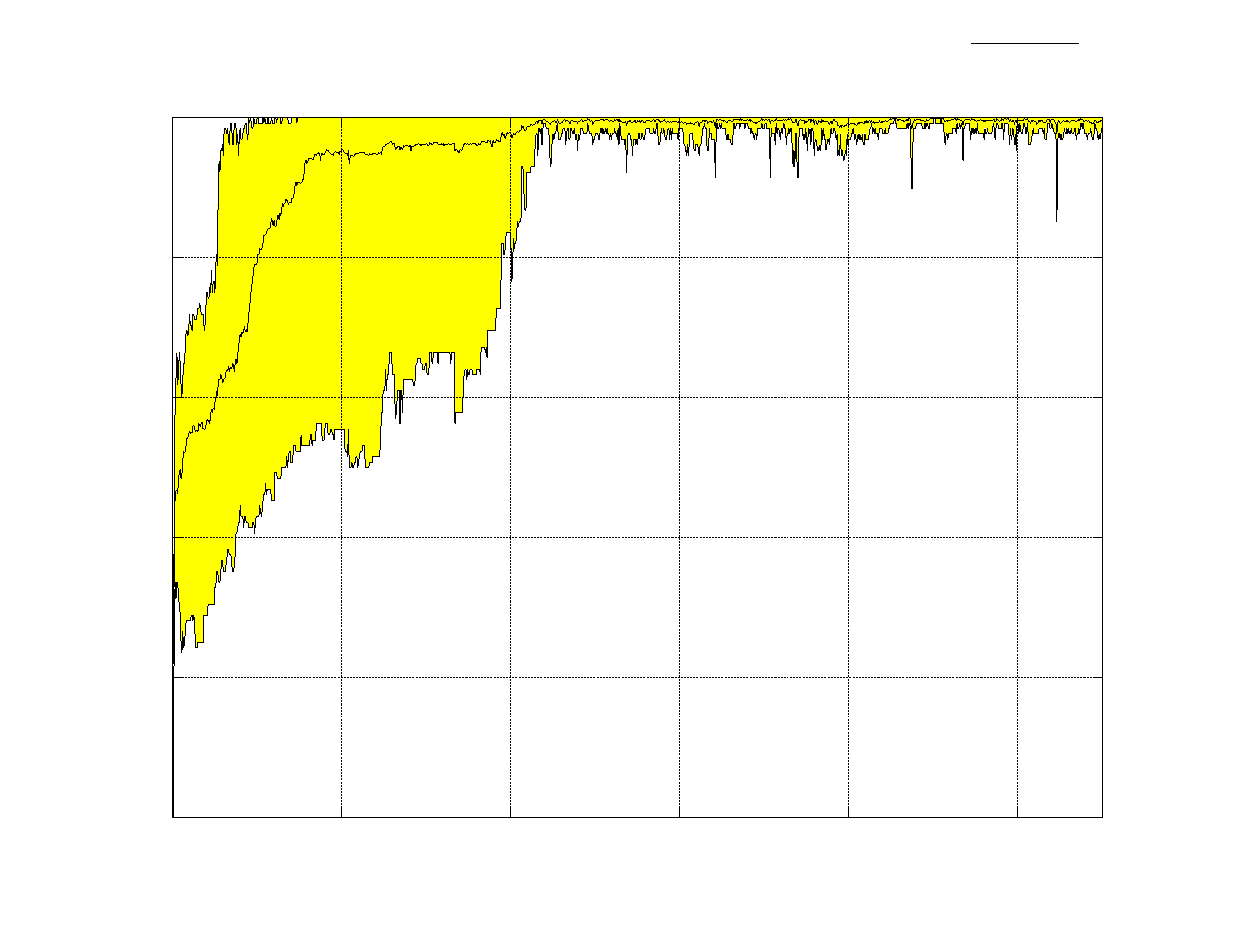
\includegraphics{./images/artificial/gmlaslcs0/identityGAex.eps}}%
    \gplfronttext
  \end{picture}%
\endgroup
}
  \put(-285,70){\rotatebox{90}{$Exact \: Match$}}
  \scalebox{0.8}{\put(-200,0){\rotatebox{0}{$iterations$}}}
  \label{fig:gmlaslcs0GAidentity7Ex}  
   
  \centering
  \scalebox{0.49}{\Large% GNUPLOT: LaTeX picture with Postscript
\begingroup
  \makeatletter
  \providecommand\color[2][]{%
    \GenericError{(gnuplot) \space\space\space\@spaces}{%
      Package color not loaded in conjunction with
      terminal option `colourtext'%
    }{See the gnuplot documentation for explanation.%
    }{Either use 'blacktext' in gnuplot or load the package
      color.sty in LaTeX.}%
    \renewcommand\color[2][]{}%
  }%
  \providecommand\includegraphics[2][]{%
    \GenericError{(gnuplot) \space\space\space\@spaces}{%
      Package graphicx or graphics not loaded%
    }{See the gnuplot documentation for explanation.%
    }{The gnuplot epslatex terminal needs graphicx.sty or graphics.sty.}%
    \renewcommand\includegraphics[2][]{}%
  }%
  \providecommand\rotatebox[2]{#2}%
  \@ifundefined{ifGPcolor}{%
    \newif\ifGPcolor
    \GPcolorfalse
  }{}%
  \@ifundefined{ifGPblacktext}{%
    \newif\ifGPblacktext
    \GPblacktexttrue
  }{}%
  % define a \g@addto@macro without @ in the name:
  \let\gplgaddtomacro\g@addto@macro
  % define empty templates for all commands taking text:
  \gdef\gplbacktext{}%
  \gdef\gplfronttext{}%
  \makeatother
  \ifGPblacktext
    % no textcolor at all
    \def\colorrgb#1{}%
    \def\colorgray#1{}%
  \else
    % gray or color?
    \ifGPcolor
      \def\colorrgb#1{\color[rgb]{#1}}%
      \def\colorgray#1{\color[gray]{#1}}%
      \expandafter\def\csname LTw\endcsname{\color{white}}%
      \expandafter\def\csname LTb\endcsname{\color{black}}%
      \expandafter\def\csname LTa\endcsname{\color{black}}%
      \expandafter\def\csname LT0\endcsname{\color[rgb]{1,0,0}}%
      \expandafter\def\csname LT1\endcsname{\color[rgb]{0,1,0}}%
      \expandafter\def\csname LT2\endcsname{\color[rgb]{0,0,1}}%
      \expandafter\def\csname LT3\endcsname{\color[rgb]{1,0,1}}%
      \expandafter\def\csname LT4\endcsname{\color[rgb]{0,1,1}}%
      \expandafter\def\csname LT5\endcsname{\color[rgb]{1,1,0}}%
      \expandafter\def\csname LT6\endcsname{\color[rgb]{0,0,0}}%
      \expandafter\def\csname LT7\endcsname{\color[rgb]{1,0.3,0}}%
      \expandafter\def\csname LT8\endcsname{\color[rgb]{0.5,0.5,0.5}}%
    \else
      % gray
      \def\colorrgb#1{\color{black}}%
      \def\colorgray#1{\color[gray]{#1}}%
      \expandafter\def\csname LTw\endcsname{\color{white}}%
      \expandafter\def\csname LTb\endcsname{\color{black}}%
      \expandafter\def\csname LTa\endcsname{\color{black}}%
      \expandafter\def\csname LT0\endcsname{\color{black}}%
      \expandafter\def\csname LT1\endcsname{\color{black}}%
      \expandafter\def\csname LT2\endcsname{\color{black}}%
      \expandafter\def\csname LT3\endcsname{\color{black}}%
      \expandafter\def\csname LT4\endcsname{\color{black}}%
      \expandafter\def\csname LT5\endcsname{\color{black}}%
      \expandafter\def\csname LT6\endcsname{\color{black}}%
      \expandafter\def\csname LT7\endcsname{\color{black}}%
      \expandafter\def\csname LT8\endcsname{\color{black}}%
    \fi
  \fi
  \setlength{\unitlength}{0.0500bp}%
  \begin{picture}(11520.00,8640.00)%
    \gplgaddtomacro\gplbacktext{%
    }%
    \gplgaddtomacro\gplfronttext{%
      \csname LTb\endcsname%
      \put(9049,8377){\makebox(0,0)[r]{\strut{}$GMl-ASLCS_{\:0GA} \: mean  \:BAM \: coverage  \:in  \:mlIdentity_7$}}%
      \colorrgb{0.00,0.00,0.00}%
      \put(1257,950){\makebox(0,0)[r]{\strut{}$0$}}%
      \colorrgb{0.00,0.00,0.00}%
      \put(1257,1622){\makebox(0,0)[r]{\strut{}$0.05$}}%
      \colorrgb{0.00,0.00,0.00}%
      \put(1257,2294){\makebox(0,0)[r]{\strut{}$0.1$}}%
      \colorrgb{0.00,0.00,0.00}%
      \put(1257,2965){\makebox(0,0)[r]{\strut{}$0.15$}}%
      \colorrgb{0.00,0.00,0.00}%
      \put(1257,3637){\makebox(0,0)[r]{\strut{}$0.2$}}%
      \colorrgb{0.00,0.00,0.00}%
      \put(1257,4309){\makebox(0,0)[r]{\strut{}$0.25$}}%
      \colorrgb{0.00,0.00,0.00}%
      \put(1257,4981){\makebox(0,0)[r]{\strut{}$0.3$}}%
      \colorrgb{0.00,0.00,0.00}%
      \put(1257,5653){\makebox(0,0)[r]{\strut{}$0.35$}}%
      \colorrgb{0.00,0.00,0.00}%
      \put(1257,6324){\makebox(0,0)[r]{\strut{}$0.4$}}%
      \colorrgb{0.00,0.00,0.00}%
      \put(1257,6996){\makebox(0,0)[r]{\strut{}$0.45$}}%
      \colorrgb{0.00,0.00,0.00}%
      \put(1257,7668){\makebox(0,0)[r]{\strut{}$0.5$}}%
      \colorrgb{0.00,0.00,0.00}%
      \put(1497,550){\makebox(0,0){\strut{}$0$}}%
      \colorrgb{0.00,0.00,0.00}%
      \put(3120,550){\makebox(0,0){\strut{}$200$}}%
      \colorrgb{0.00,0.00,0.00}%
      \put(4743,550){\makebox(0,0){\strut{}$400$}}%
      \colorrgb{0.00,0.00,0.00}%
      \put(6366,550){\makebox(0,0){\strut{}$600$}}%
      \colorrgb{0.00,0.00,0.00}%
      \put(7989,550){\makebox(0,0){\strut{}$800$}}%
      \colorrgb{0.00,0.00,0.00}%
      \put(9612,550){\makebox(0,0){\strut{}$1000$}}%
    }%
    \gplbacktext
    \put(0,0){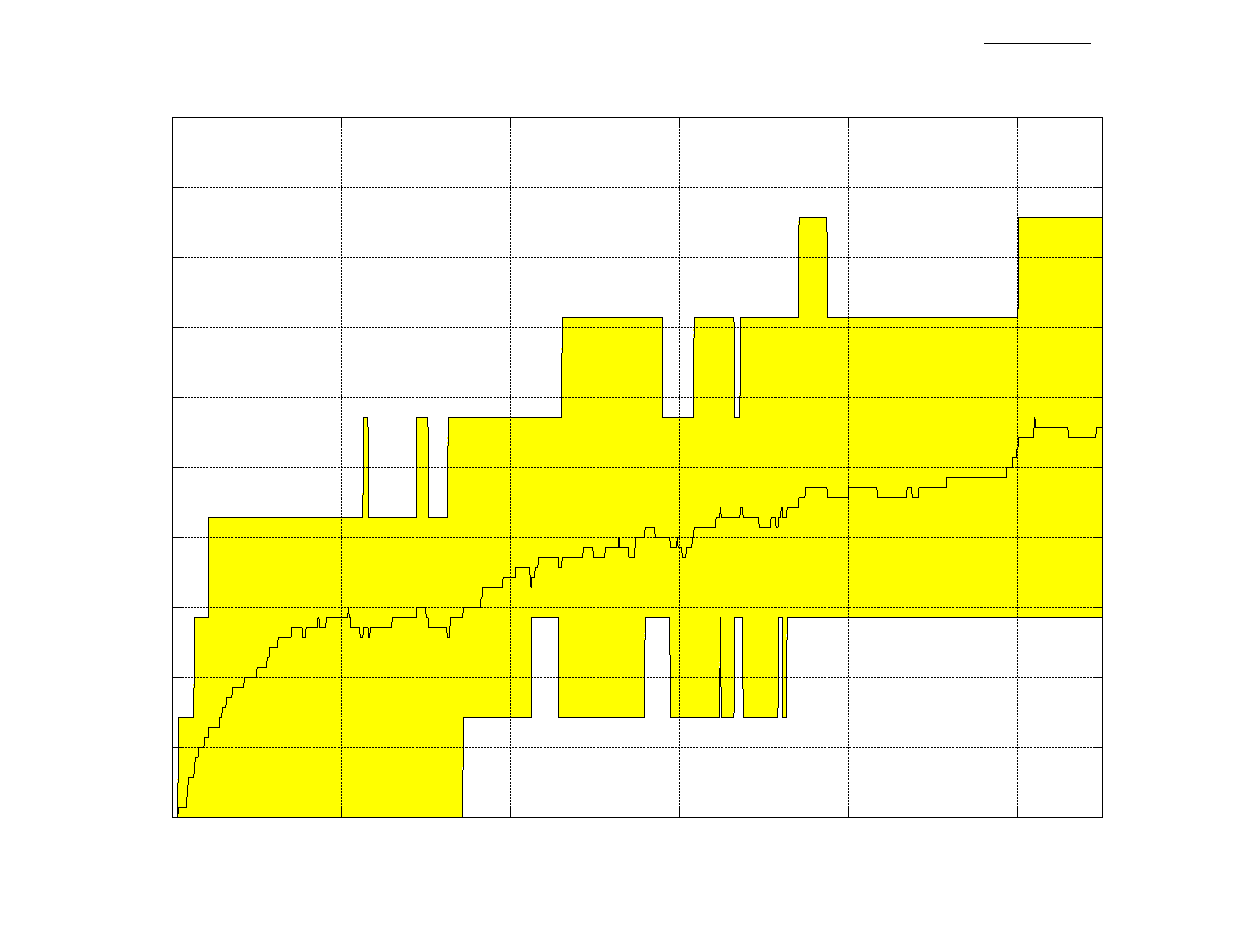
\includegraphics{./images/artificial/gmlaslcs0/identityGABAM.eps}}%
    \gplfronttext
  \end{picture}%
\endgroup
}
  \put(-285,80){\rotatebox{90}{$BAM$}}
  \scalebox{0.8}{\put(-200,0){\rotatebox{0}{$iterations$}}}
  \label{fig:gmlaslcs0GAidentity7BAM} 
\end{figure}

\begin{figure}[ht]
  \caption{Διαγράμματα χαρτογράφησης $mlIdentity_{7}$ του GMl-ASLCS$_{\:0M}$.}
  \label{fig:gmlaslcs0Midentity7}
  \centering
  \scalebox{0.49}{\Large% GNUPLOT: LaTeX picture with Postscript
\begingroup
  \makeatletter
  \providecommand\color[2][]{%
    \GenericError{(gnuplot) \space\space\space\@spaces}{%
      Package color not loaded in conjunction with
      terminal option `colourtext'%
    }{See the gnuplot documentation for explanation.%
    }{Either use 'blacktext' in gnuplot or load the package
      color.sty in LaTeX.}%
    \renewcommand\color[2][]{}%
  }%
  \providecommand\includegraphics[2][]{%
    \GenericError{(gnuplot) \space\space\space\@spaces}{%
      Package graphicx or graphics not loaded%
    }{See the gnuplot documentation for explanation.%
    }{The gnuplot epslatex terminal needs graphicx.sty or graphics.sty.}%
    \renewcommand\includegraphics[2][]{}%
  }%
  \providecommand\rotatebox[2]{#2}%
  \@ifundefined{ifGPcolor}{%
    \newif\ifGPcolor
    \GPcolorfalse
  }{}%
  \@ifundefined{ifGPblacktext}{%
    \newif\ifGPblacktext
    \GPblacktexttrue
  }{}%
  % define a \g@addto@macro without @ in the name:
  \let\gplgaddtomacro\g@addto@macro
  % define empty templates for all commands taking text:
  \gdef\gplbacktext{}%
  \gdef\gplfronttext{}%
  \makeatother
  \ifGPblacktext
    % no textcolor at all
    \def\colorrgb#1{}%
    \def\colorgray#1{}%
  \else
    % gray or color?
    \ifGPcolor
      \def\colorrgb#1{\color[rgb]{#1}}%
      \def\colorgray#1{\color[gray]{#1}}%
      \expandafter\def\csname LTw\endcsname{\color{white}}%
      \expandafter\def\csname LTb\endcsname{\color{black}}%
      \expandafter\def\csname LTa\endcsname{\color{black}}%
      \expandafter\def\csname LT0\endcsname{\color[rgb]{1,0,0}}%
      \expandafter\def\csname LT1\endcsname{\color[rgb]{0,1,0}}%
      \expandafter\def\csname LT2\endcsname{\color[rgb]{0,0,1}}%
      \expandafter\def\csname LT3\endcsname{\color[rgb]{1,0,1}}%
      \expandafter\def\csname LT4\endcsname{\color[rgb]{0,1,1}}%
      \expandafter\def\csname LT5\endcsname{\color[rgb]{1,1,0}}%
      \expandafter\def\csname LT6\endcsname{\color[rgb]{0,0,0}}%
      \expandafter\def\csname LT7\endcsname{\color[rgb]{1,0.3,0}}%
      \expandafter\def\csname LT8\endcsname{\color[rgb]{0.5,0.5,0.5}}%
    \else
      % gray
      \def\colorrgb#1{\color{black}}%
      \def\colorgray#1{\color[gray]{#1}}%
      \expandafter\def\csname LTw\endcsname{\color{white}}%
      \expandafter\def\csname LTb\endcsname{\color{black}}%
      \expandafter\def\csname LTa\endcsname{\color{black}}%
      \expandafter\def\csname LT0\endcsname{\color{black}}%
      \expandafter\def\csname LT1\endcsname{\color{black}}%
      \expandafter\def\csname LT2\endcsname{\color{black}}%
      \expandafter\def\csname LT3\endcsname{\color{black}}%
      \expandafter\def\csname LT4\endcsname{\color{black}}%
      \expandafter\def\csname LT5\endcsname{\color{black}}%
      \expandafter\def\csname LT6\endcsname{\color{black}}%
      \expandafter\def\csname LT7\endcsname{\color{black}}%
      \expandafter\def\csname LT8\endcsname{\color{black}}%
    \fi
  \fi
  \setlength{\unitlength}{0.0500bp}%
  \begin{picture}(11520.00,8640.00)%
    \gplgaddtomacro\gplbacktext{%
    }%
    \gplgaddtomacro\gplfronttext{%
      \csname LTb\endcsname%
      \put(8569,8377){\makebox(0,0)[r]{\strut{}$GMl-ASLCS_{\:0M} \: mean \: accuracy \: in \: mlIdentity_7$}}%
      \colorrgb{0.00,0.00,0.00}%
      \put(1257,950){\makebox(0,0)[r]{\strut{}$0$}}%
      \colorrgb{0.00,0.00,0.00}%
      \put(1257,2294){\makebox(0,0)[r]{\strut{}$0.2$}}%
      \colorrgb{0.00,0.00,0.00}%
      \put(1257,3637){\makebox(0,0)[r]{\strut{}$0.4$}}%
      \colorrgb{0.00,0.00,0.00}%
      \put(1257,4981){\makebox(0,0)[r]{\strut{}$0.6$}}%
      \colorrgb{0.00,0.00,0.00}%
      \put(1257,6324){\makebox(0,0)[r]{\strut{}$0.8$}}%
      \colorrgb{0.00,0.00,0.00}%
      \put(1257,7668){\makebox(0,0)[r]{\strut{}$1$}}%
      \colorrgb{0.00,0.00,0.00}%
      \put(1497,550){\makebox(0,0){\strut{}$0$}}%
      \colorrgb{0.00,0.00,0.00}%
      \put(3120,550){\makebox(0,0){\strut{}$200$}}%
      \colorrgb{0.00,0.00,0.00}%
      \put(4743,550){\makebox(0,0){\strut{}$400$}}%
      \colorrgb{0.00,0.00,0.00}%
      \put(6366,550){\makebox(0,0){\strut{}$600$}}%
      \colorrgb{0.00,0.00,0.00}%
      \put(7989,550){\makebox(0,0){\strut{}$800$}}%
      \colorrgb{0.00,0.00,0.00}%
      \put(9612,550){\makebox(0,0){\strut{}$1000$}}%
    }%
    \gplbacktext
    \put(0,0){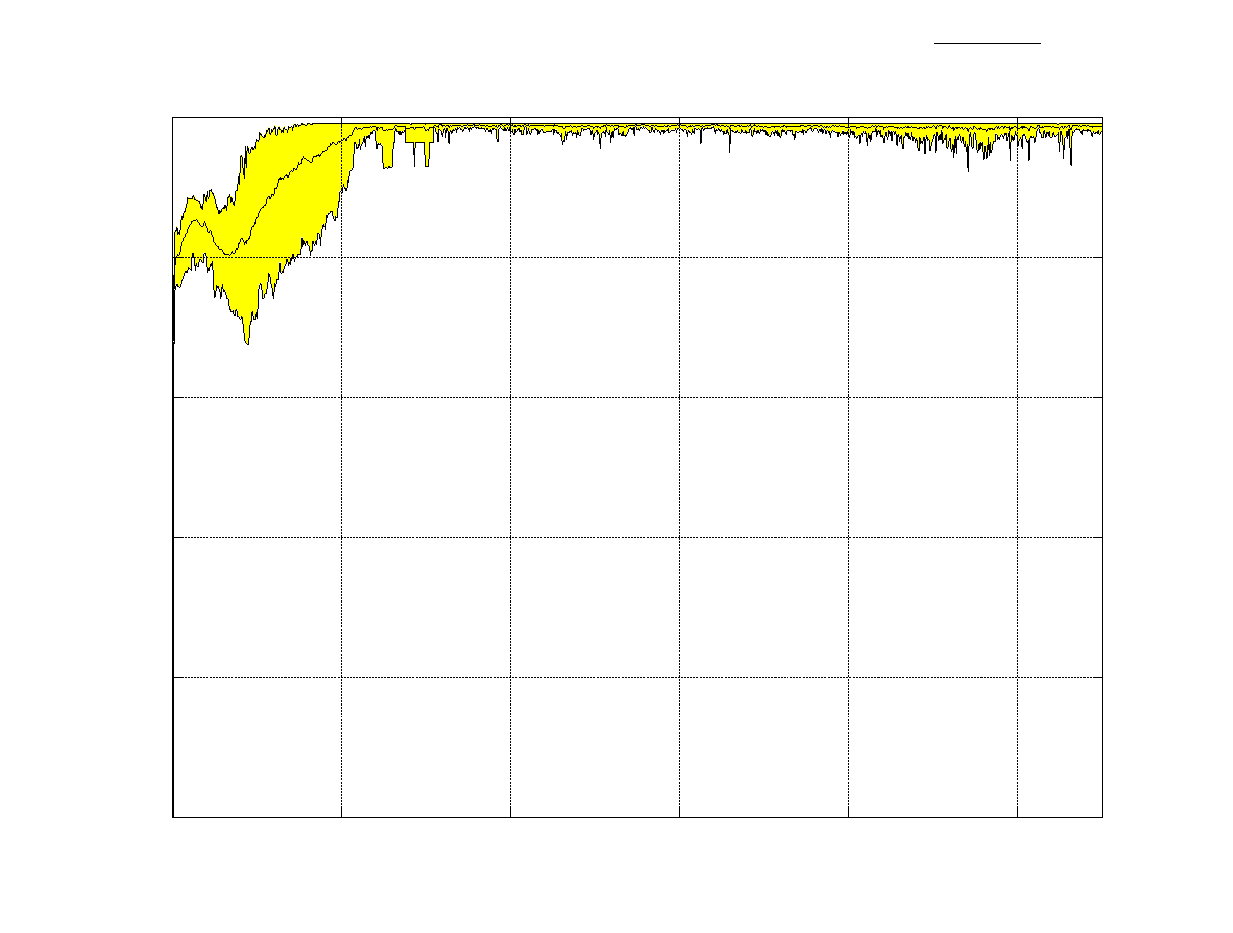
\includegraphics{./images/artificial/gmlaslcs0/identityMacc.eps}}%
    \gplfronttext
  \end{picture}%
\endgroup
}
  \put(-285,70){\rotatebox{90}{$Accuracy$}}
  \scalebox{0.8}{\put(-200,0){\rotatebox{0}{$iterations$}}}
  \label{fig:gmlaslcs0Midentity7Acc} 
  
  \centering
  \scalebox{0.49}{\Large% GNUPLOT: LaTeX picture with Postscript
\begingroup
  \makeatletter
  \providecommand\color[2][]{%
    \GenericError{(gnuplot) \space\space\space\@spaces}{%
      Package color not loaded in conjunction with
      terminal option `colourtext'%
    }{See the gnuplot documentation for explanation.%
    }{Either use 'blacktext' in gnuplot or load the package
      color.sty in LaTeX.}%
    \renewcommand\color[2][]{}%
  }%
  \providecommand\includegraphics[2][]{%
    \GenericError{(gnuplot) \space\space\space\@spaces}{%
      Package graphicx or graphics not loaded%
    }{See the gnuplot documentation for explanation.%
    }{The gnuplot epslatex terminal needs graphicx.sty or graphics.sty.}%
    \renewcommand\includegraphics[2][]{}%
  }%
  \providecommand\rotatebox[2]{#2}%
  \@ifundefined{ifGPcolor}{%
    \newif\ifGPcolor
    \GPcolorfalse
  }{}%
  \@ifundefined{ifGPblacktext}{%
    \newif\ifGPblacktext
    \GPblacktexttrue
  }{}%
  % define a \g@addto@macro without @ in the name:
  \let\gplgaddtomacro\g@addto@macro
  % define empty templates for all commands taking text:
  \gdef\gplbacktext{}%
  \gdef\gplfronttext{}%
  \makeatother
  \ifGPblacktext
    % no textcolor at all
    \def\colorrgb#1{}%
    \def\colorgray#1{}%
  \else
    % gray or color?
    \ifGPcolor
      \def\colorrgb#1{\color[rgb]{#1}}%
      \def\colorgray#1{\color[gray]{#1}}%
      \expandafter\def\csname LTw\endcsname{\color{white}}%
      \expandafter\def\csname LTb\endcsname{\color{black}}%
      \expandafter\def\csname LTa\endcsname{\color{black}}%
      \expandafter\def\csname LT0\endcsname{\color[rgb]{1,0,0}}%
      \expandafter\def\csname LT1\endcsname{\color[rgb]{0,1,0}}%
      \expandafter\def\csname LT2\endcsname{\color[rgb]{0,0,1}}%
      \expandafter\def\csname LT3\endcsname{\color[rgb]{1,0,1}}%
      \expandafter\def\csname LT4\endcsname{\color[rgb]{0,1,1}}%
      \expandafter\def\csname LT5\endcsname{\color[rgb]{1,1,0}}%
      \expandafter\def\csname LT6\endcsname{\color[rgb]{0,0,0}}%
      \expandafter\def\csname LT7\endcsname{\color[rgb]{1,0.3,0}}%
      \expandafter\def\csname LT8\endcsname{\color[rgb]{0.5,0.5,0.5}}%
    \else
      % gray
      \def\colorrgb#1{\color{black}}%
      \def\colorgray#1{\color[gray]{#1}}%
      \expandafter\def\csname LTw\endcsname{\color{white}}%
      \expandafter\def\csname LTb\endcsname{\color{black}}%
      \expandafter\def\csname LTa\endcsname{\color{black}}%
      \expandafter\def\csname LT0\endcsname{\color{black}}%
      \expandafter\def\csname LT1\endcsname{\color{black}}%
      \expandafter\def\csname LT2\endcsname{\color{black}}%
      \expandafter\def\csname LT3\endcsname{\color{black}}%
      \expandafter\def\csname LT4\endcsname{\color{black}}%
      \expandafter\def\csname LT5\endcsname{\color{black}}%
      \expandafter\def\csname LT6\endcsname{\color{black}}%
      \expandafter\def\csname LT7\endcsname{\color{black}}%
      \expandafter\def\csname LT8\endcsname{\color{black}}%
    \fi
  \fi
  \setlength{\unitlength}{0.0500bp}%
  \begin{picture}(11520.00,8640.00)%
    \gplgaddtomacro\gplbacktext{%
    }%
    \gplgaddtomacro\gplfronttext{%
      \csname LTb\endcsname%
      \put(8929,8377){\makebox(0,0)[r]{\strut{}$GMl-ASLCS_{\:0M} \: mean \: exact  \:match \: in \: mlIdentity_7$}}%
      \colorrgb{0.00,0.00,0.00}%
      \put(1257,950){\makebox(0,0)[r]{\strut{}$0$}}%
      \colorrgb{0.00,0.00,0.00}%
      \put(1257,2294){\makebox(0,0)[r]{\strut{}$0.2$}}%
      \colorrgb{0.00,0.00,0.00}%
      \put(1257,3637){\makebox(0,0)[r]{\strut{}$0.4$}}%
      \colorrgb{0.00,0.00,0.00}%
      \put(1257,4981){\makebox(0,0)[r]{\strut{}$0.6$}}%
      \colorrgb{0.00,0.00,0.00}%
      \put(1257,6324){\makebox(0,0)[r]{\strut{}$0.8$}}%
      \colorrgb{0.00,0.00,0.00}%
      \put(1257,7668){\makebox(0,0)[r]{\strut{}$1$}}%
      \colorrgb{0.00,0.00,0.00}%
      \put(1497,550){\makebox(0,0){\strut{}$0$}}%
      \colorrgb{0.00,0.00,0.00}%
      \put(3120,550){\makebox(0,0){\strut{}$200$}}%
      \colorrgb{0.00,0.00,0.00}%
      \put(4743,550){\makebox(0,0){\strut{}$400$}}%
      \colorrgb{0.00,0.00,0.00}%
      \put(6366,550){\makebox(0,0){\strut{}$600$}}%
      \colorrgb{0.00,0.00,0.00}%
      \put(7989,550){\makebox(0,0){\strut{}$800$}}%
      \colorrgb{0.00,0.00,0.00}%
      \put(9612,550){\makebox(0,0){\strut{}$1000$}}%
    }%
    \gplbacktext
    \put(0,0){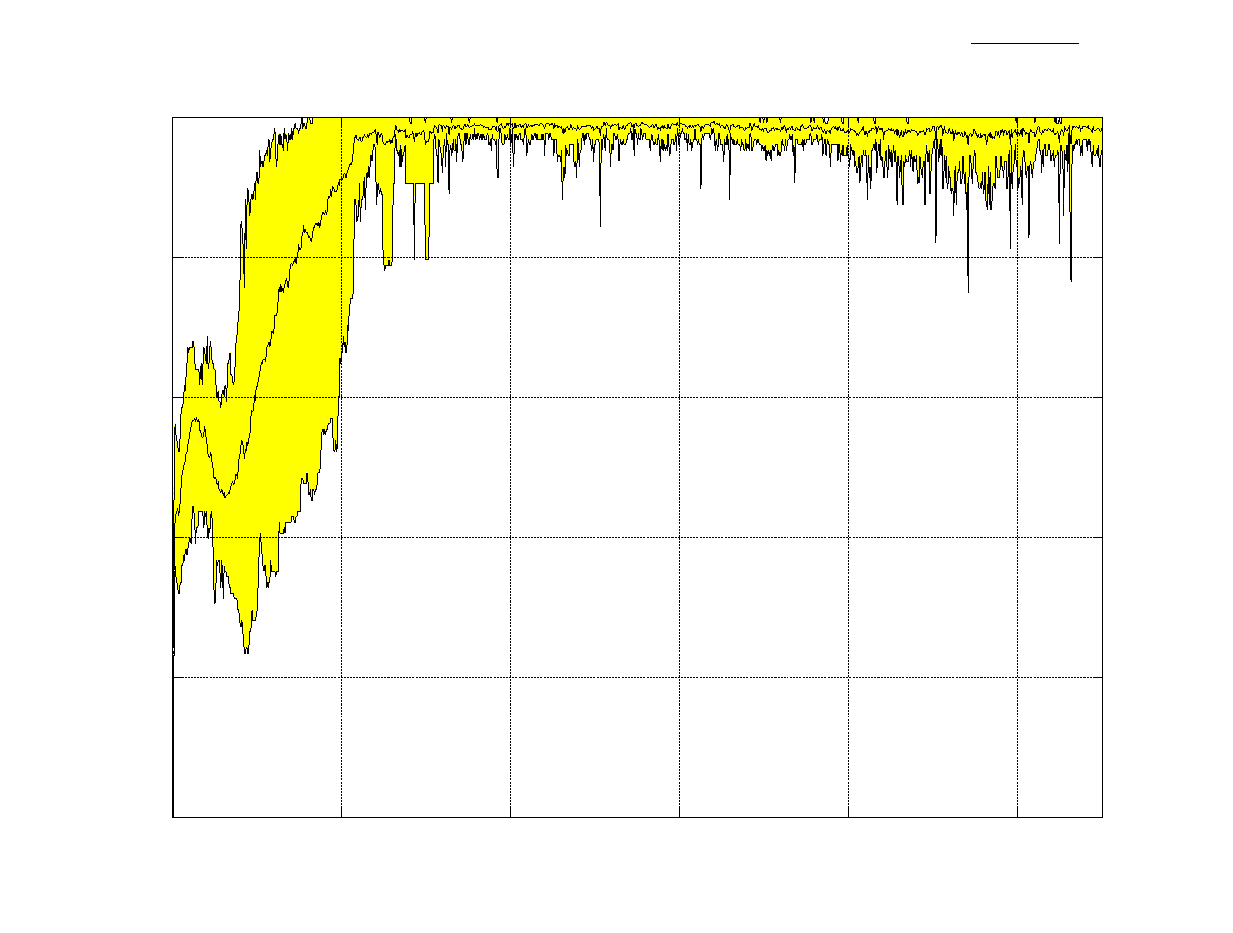
\includegraphics{./images/artificial/gmlaslcs0/identityMex.eps}}%
    \gplfronttext
  \end{picture}%
\endgroup
}
  \put(-285,70){\rotatebox{90}{$Exact \: Match$}}
  \scalebox{0.8}{\put(-200,0){\rotatebox{0}{$iterations$}}}
  \label{fig:gmlaslcs0Midentity7Ex}  
   
  \centering
  \scalebox{0.49}{\Large% GNUPLOT: LaTeX picture with Postscript
\begingroup
  \makeatletter
  \providecommand\color[2][]{%
    \GenericError{(gnuplot) \space\space\space\@spaces}{%
      Package color not loaded in conjunction with
      terminal option `colourtext'%
    }{See the gnuplot documentation for explanation.%
    }{Either use 'blacktext' in gnuplot or load the package
      color.sty in LaTeX.}%
    \renewcommand\color[2][]{}%
  }%
  \providecommand\includegraphics[2][]{%
    \GenericError{(gnuplot) \space\space\space\@spaces}{%
      Package graphicx or graphics not loaded%
    }{See the gnuplot documentation for explanation.%
    }{The gnuplot epslatex terminal needs graphicx.sty or graphics.sty.}%
    \renewcommand\includegraphics[2][]{}%
  }%
  \providecommand\rotatebox[2]{#2}%
  \@ifundefined{ifGPcolor}{%
    \newif\ifGPcolor
    \GPcolorfalse
  }{}%
  \@ifundefined{ifGPblacktext}{%
    \newif\ifGPblacktext
    \GPblacktexttrue
  }{}%
  % define a \g@addto@macro without @ in the name:
  \let\gplgaddtomacro\g@addto@macro
  % define empty templates for all commands taking text:
  \gdef\gplbacktext{}%
  \gdef\gplfronttext{}%
  \makeatother
  \ifGPblacktext
    % no textcolor at all
    \def\colorrgb#1{}%
    \def\colorgray#1{}%
  \else
    % gray or color?
    \ifGPcolor
      \def\colorrgb#1{\color[rgb]{#1}}%
      \def\colorgray#1{\color[gray]{#1}}%
      \expandafter\def\csname LTw\endcsname{\color{white}}%
      \expandafter\def\csname LTb\endcsname{\color{black}}%
      \expandafter\def\csname LTa\endcsname{\color{black}}%
      \expandafter\def\csname LT0\endcsname{\color[rgb]{1,0,0}}%
      \expandafter\def\csname LT1\endcsname{\color[rgb]{0,1,0}}%
      \expandafter\def\csname LT2\endcsname{\color[rgb]{0,0,1}}%
      \expandafter\def\csname LT3\endcsname{\color[rgb]{1,0,1}}%
      \expandafter\def\csname LT4\endcsname{\color[rgb]{0,1,1}}%
      \expandafter\def\csname LT5\endcsname{\color[rgb]{1,1,0}}%
      \expandafter\def\csname LT6\endcsname{\color[rgb]{0,0,0}}%
      \expandafter\def\csname LT7\endcsname{\color[rgb]{1,0.3,0}}%
      \expandafter\def\csname LT8\endcsname{\color[rgb]{0.5,0.5,0.5}}%
    \else
      % gray
      \def\colorrgb#1{\color{black}}%
      \def\colorgray#1{\color[gray]{#1}}%
      \expandafter\def\csname LTw\endcsname{\color{white}}%
      \expandafter\def\csname LTb\endcsname{\color{black}}%
      \expandafter\def\csname LTa\endcsname{\color{black}}%
      \expandafter\def\csname LT0\endcsname{\color{black}}%
      \expandafter\def\csname LT1\endcsname{\color{black}}%
      \expandafter\def\csname LT2\endcsname{\color{black}}%
      \expandafter\def\csname LT3\endcsname{\color{black}}%
      \expandafter\def\csname LT4\endcsname{\color{black}}%
      \expandafter\def\csname LT5\endcsname{\color{black}}%
      \expandafter\def\csname LT6\endcsname{\color{black}}%
      \expandafter\def\csname LT7\endcsname{\color{black}}%
      \expandafter\def\csname LT8\endcsname{\color{black}}%
    \fi
  \fi
  \setlength{\unitlength}{0.0500bp}%
  \begin{picture}(11520.00,8640.00)%
    \gplgaddtomacro\gplbacktext{%
    }%
    \gplgaddtomacro\gplfronttext{%
      \csname LTb\endcsname%
      \put(9049,8377){\makebox(0,0)[r]{\strut{}$GMl-ASLCS_{\:0M} \: mean \: BAM \: coverage \: in \: mlIdentity_7$}}%
      \colorrgb{0.00,0.00,0.00}%
      \put(1257,950){\makebox(0,0)[r]{\strut{}$0$}}%
      \colorrgb{0.00,0.00,0.00}%
      \put(1257,1622){\makebox(0,0)[r]{\strut{}$0.05$}}%
      \colorrgb{0.00,0.00,0.00}%
      \put(1257,2294){\makebox(0,0)[r]{\strut{}$0.1$}}%
      \colorrgb{0.00,0.00,0.00}%
      \put(1257,2965){\makebox(0,0)[r]{\strut{}$0.15$}}%
      \colorrgb{0.00,0.00,0.00}%
      \put(1257,3637){\makebox(0,0)[r]{\strut{}$0.2$}}%
      \colorrgb{0.00,0.00,0.00}%
      \put(1257,4309){\makebox(0,0)[r]{\strut{}$0.25$}}%
      \colorrgb{0.00,0.00,0.00}%
      \put(1257,4981){\makebox(0,0)[r]{\strut{}$0.3$}}%
      \colorrgb{0.00,0.00,0.00}%
      \put(1257,5653){\makebox(0,0)[r]{\strut{}$0.35$}}%
      \colorrgb{0.00,0.00,0.00}%
      \put(1257,6324){\makebox(0,0)[r]{\strut{}$0.4$}}%
      \colorrgb{0.00,0.00,0.00}%
      \put(1257,6996){\makebox(0,0)[r]{\strut{}$0.45$}}%
      \colorrgb{0.00,0.00,0.00}%
      \put(1257,7668){\makebox(0,0)[r]{\strut{}$0.5$}}%
      \colorrgb{0.00,0.00,0.00}%
      \put(1497,550){\makebox(0,0){\strut{}$0$}}%
      \colorrgb{0.00,0.00,0.00}%
      \put(3120,550){\makebox(0,0){\strut{}$200$}}%
      \colorrgb{0.00,0.00,0.00}%
      \put(4743,550){\makebox(0,0){\strut{}$400$}}%
      \colorrgb{0.00,0.00,0.00}%
      \put(6366,550){\makebox(0,0){\strut{}$600$}}%
      \colorrgb{0.00,0.00,0.00}%
      \put(7989,550){\makebox(0,0){\strut{}$800$}}%
      \colorrgb{0.00,0.00,0.00}%
      \put(9612,550){\makebox(0,0){\strut{}$1000$}}%
    }%
    \gplbacktext
    \put(0,0){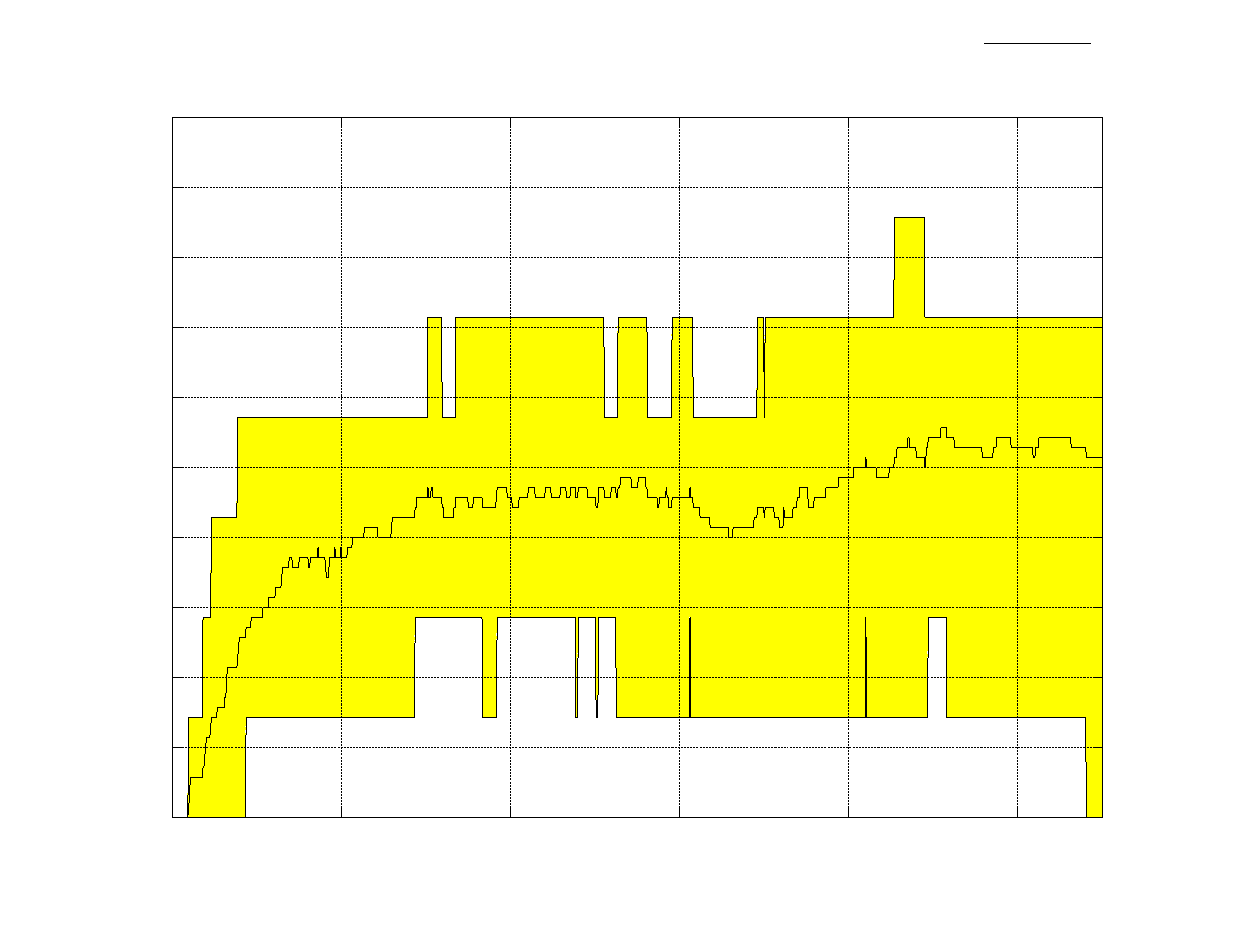
\includegraphics{./images/artificial/gmlaslcs0/identityMBAM.eps}}%
    \gplfronttext
  \end{picture}%
\endgroup
}
  \put(-285,80){\rotatebox{90}{$BAM$}}
  \scalebox{0.8}{\put(-200,0){\rotatebox{0}{$iterations$}}}
  \label{fig:gmlaslcs0Midentity7BAM} 
\end{figure}

\begin{figure}[ht]
  \caption{Διαγράμματα χαρτογράφησης $mlIdentity_{7}$ του GMl-ASLCS$_{\:0C}$.}
  \label{fig:gmlaslcs0Cidentity7}
  \centering
  \scalebox{0.49}{\Large% GNUPLOT: LaTeX picture with Postscript
\begingroup
  \makeatletter
  \providecommand\color[2][]{%
    \GenericError{(gnuplot) \space\space\space\@spaces}{%
      Package color not loaded in conjunction with
      terminal option `colourtext'%
    }{See the gnuplot documentation for explanation.%
    }{Either use 'blacktext' in gnuplot or load the package
      color.sty in LaTeX.}%
    \renewcommand\color[2][]{}%
  }%
  \providecommand\includegraphics[2][]{%
    \GenericError{(gnuplot) \space\space\space\@spaces}{%
      Package graphicx or graphics not loaded%
    }{See the gnuplot documentation for explanation.%
    }{The gnuplot epslatex terminal needs graphicx.sty or graphics.sty.}%
    \renewcommand\includegraphics[2][]{}%
  }%
  \providecommand\rotatebox[2]{#2}%
  \@ifundefined{ifGPcolor}{%
    \newif\ifGPcolor
    \GPcolorfalse
  }{}%
  \@ifundefined{ifGPblacktext}{%
    \newif\ifGPblacktext
    \GPblacktexttrue
  }{}%
  % define a \g@addto@macro without @ in the name:
  \let\gplgaddtomacro\g@addto@macro
  % define empty templates for all commands taking text:
  \gdef\gplbacktext{}%
  \gdef\gplfronttext{}%
  \makeatother
  \ifGPblacktext
    % no textcolor at all
    \def\colorrgb#1{}%
    \def\colorgray#1{}%
  \else
    % gray or color?
    \ifGPcolor
      \def\colorrgb#1{\color[rgb]{#1}}%
      \def\colorgray#1{\color[gray]{#1}}%
      \expandafter\def\csname LTw\endcsname{\color{white}}%
      \expandafter\def\csname LTb\endcsname{\color{black}}%
      \expandafter\def\csname LTa\endcsname{\color{black}}%
      \expandafter\def\csname LT0\endcsname{\color[rgb]{1,0,0}}%
      \expandafter\def\csname LT1\endcsname{\color[rgb]{0,1,0}}%
      \expandafter\def\csname LT2\endcsname{\color[rgb]{0,0,1}}%
      \expandafter\def\csname LT3\endcsname{\color[rgb]{1,0,1}}%
      \expandafter\def\csname LT4\endcsname{\color[rgb]{0,1,1}}%
      \expandafter\def\csname LT5\endcsname{\color[rgb]{1,1,0}}%
      \expandafter\def\csname LT6\endcsname{\color[rgb]{0,0,0}}%
      \expandafter\def\csname LT7\endcsname{\color[rgb]{1,0.3,0}}%
      \expandafter\def\csname LT8\endcsname{\color[rgb]{0.5,0.5,0.5}}%
    \else
      % gray
      \def\colorrgb#1{\color{black}}%
      \def\colorgray#1{\color[gray]{#1}}%
      \expandafter\def\csname LTw\endcsname{\color{white}}%
      \expandafter\def\csname LTb\endcsname{\color{black}}%
      \expandafter\def\csname LTa\endcsname{\color{black}}%
      \expandafter\def\csname LT0\endcsname{\color{black}}%
      \expandafter\def\csname LT1\endcsname{\color{black}}%
      \expandafter\def\csname LT2\endcsname{\color{black}}%
      \expandafter\def\csname LT3\endcsname{\color{black}}%
      \expandafter\def\csname LT4\endcsname{\color{black}}%
      \expandafter\def\csname LT5\endcsname{\color{black}}%
      \expandafter\def\csname LT6\endcsname{\color{black}}%
      \expandafter\def\csname LT7\endcsname{\color{black}}%
      \expandafter\def\csname LT8\endcsname{\color{black}}%
    \fi
  \fi
  \setlength{\unitlength}{0.0500bp}%
  \begin{picture}(11520.00,8640.00)%
    \gplgaddtomacro\gplbacktext{%
    }%
    \gplgaddtomacro\gplfronttext{%
      \csname LTb\endcsname%
      \put(8569,8377){\makebox(0,0)[r]{\strut{}$GMl-ASLCS_{\:0C} \: mean \: accuracy  \:in \: mlIdentity_7$}}%
      \colorrgb{0.00,0.00,0.00}%
      \put(1257,950){\makebox(0,0)[r]{\strut{}$0$}}%
      \colorrgb{0.00,0.00,0.00}%
      \put(1257,2294){\makebox(0,0)[r]{\strut{}$0.2$}}%
      \colorrgb{0.00,0.00,0.00}%
      \put(1257,3637){\makebox(0,0)[r]{\strut{}$0.4$}}%
      \colorrgb{0.00,0.00,0.00}%
      \put(1257,4981){\makebox(0,0)[r]{\strut{}$0.6$}}%
      \colorrgb{0.00,0.00,0.00}%
      \put(1257,6324){\makebox(0,0)[r]{\strut{}$0.8$}}%
      \colorrgb{0.00,0.00,0.00}%
      \put(1257,7668){\makebox(0,0)[r]{\strut{}$1$}}%
      \colorrgb{0.00,0.00,0.00}%
      \put(1497,550){\makebox(0,0){\strut{}$0$}}%
      \colorrgb{0.00,0.00,0.00}%
      \put(3120,550){\makebox(0,0){\strut{}$200$}}%
      \colorrgb{0.00,0.00,0.00}%
      \put(4743,550){\makebox(0,0){\strut{}$400$}}%
      \colorrgb{0.00,0.00,0.00}%
      \put(6366,550){\makebox(0,0){\strut{}$600$}}%
      \colorrgb{0.00,0.00,0.00}%
      \put(7989,550){\makebox(0,0){\strut{}$800$}}%
      \colorrgb{0.00,0.00,0.00}%
      \put(9612,550){\makebox(0,0){\strut{}$1000$}}%
    }%
    \gplbacktext
    \put(0,0){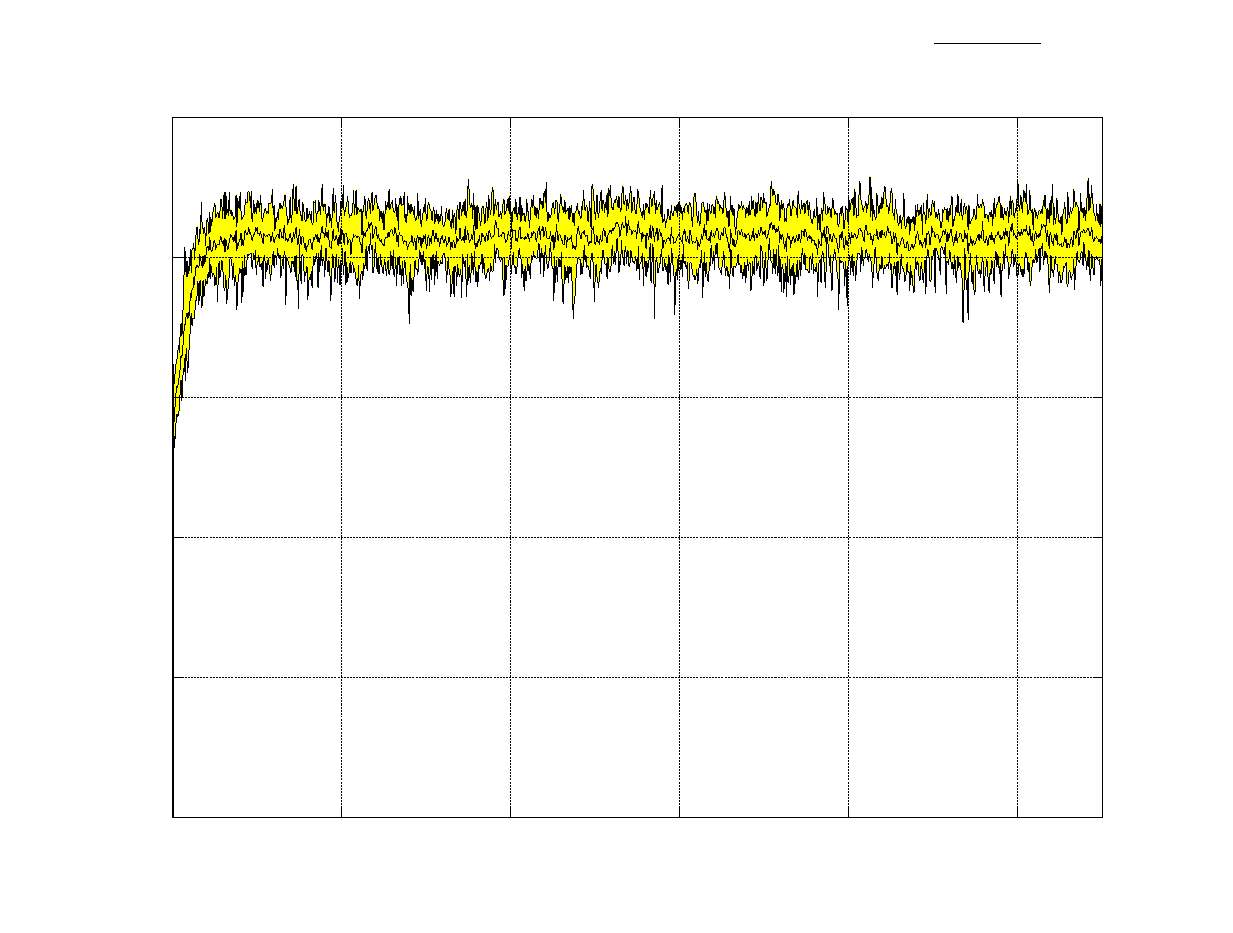
\includegraphics{./images/artificial/gmlaslcs0/identityCacc.eps}}%
    \gplfronttext
  \end{picture}%
\endgroup
}
  \put(-285,70){\rotatebox{90}{$Accuracy$}}
  \scalebox{0.8}{\put(-200,0){\rotatebox{0}{$iterations$}}}
  \label{fig:gmlaslcs0Cidentity7Acc} 
  
  \centering
  \scalebox{0.49}{\Large% GNUPLOT: LaTeX picture with Postscript
\begingroup
  \makeatletter
  \providecommand\color[2][]{%
    \GenericError{(gnuplot) \space\space\space\@spaces}{%
      Package color not loaded in conjunction with
      terminal option `colourtext'%
    }{See the gnuplot documentation for explanation.%
    }{Either use 'blacktext' in gnuplot or load the package
      color.sty in LaTeX.}%
    \renewcommand\color[2][]{}%
  }%
  \providecommand\includegraphics[2][]{%
    \GenericError{(gnuplot) \space\space\space\@spaces}{%
      Package graphicx or graphics not loaded%
    }{See the gnuplot documentation for explanation.%
    }{The gnuplot epslatex terminal needs graphicx.sty or graphics.sty.}%
    \renewcommand\includegraphics[2][]{}%
  }%
  \providecommand\rotatebox[2]{#2}%
  \@ifundefined{ifGPcolor}{%
    \newif\ifGPcolor
    \GPcolorfalse
  }{}%
  \@ifundefined{ifGPblacktext}{%
    \newif\ifGPblacktext
    \GPblacktexttrue
  }{}%
  % define a \g@addto@macro without @ in the name:
  \let\gplgaddtomacro\g@addto@macro
  % define empty templates for all commands taking text:
  \gdef\gplbacktext{}%
  \gdef\gplfronttext{}%
  \makeatother
  \ifGPblacktext
    % no textcolor at all
    \def\colorrgb#1{}%
    \def\colorgray#1{}%
  \else
    % gray or color?
    \ifGPcolor
      \def\colorrgb#1{\color[rgb]{#1}}%
      \def\colorgray#1{\color[gray]{#1}}%
      \expandafter\def\csname LTw\endcsname{\color{white}}%
      \expandafter\def\csname LTb\endcsname{\color{black}}%
      \expandafter\def\csname LTa\endcsname{\color{black}}%
      \expandafter\def\csname LT0\endcsname{\color[rgb]{1,0,0}}%
      \expandafter\def\csname LT1\endcsname{\color[rgb]{0,1,0}}%
      \expandafter\def\csname LT2\endcsname{\color[rgb]{0,0,1}}%
      \expandafter\def\csname LT3\endcsname{\color[rgb]{1,0,1}}%
      \expandafter\def\csname LT4\endcsname{\color[rgb]{0,1,1}}%
      \expandafter\def\csname LT5\endcsname{\color[rgb]{1,1,0}}%
      \expandafter\def\csname LT6\endcsname{\color[rgb]{0,0,0}}%
      \expandafter\def\csname LT7\endcsname{\color[rgb]{1,0.3,0}}%
      \expandafter\def\csname LT8\endcsname{\color[rgb]{0.5,0.5,0.5}}%
    \else
      % gray
      \def\colorrgb#1{\color{black}}%
      \def\colorgray#1{\color[gray]{#1}}%
      \expandafter\def\csname LTw\endcsname{\color{white}}%
      \expandafter\def\csname LTb\endcsname{\color{black}}%
      \expandafter\def\csname LTa\endcsname{\color{black}}%
      \expandafter\def\csname LT0\endcsname{\color{black}}%
      \expandafter\def\csname LT1\endcsname{\color{black}}%
      \expandafter\def\csname LT2\endcsname{\color{black}}%
      \expandafter\def\csname LT3\endcsname{\color{black}}%
      \expandafter\def\csname LT4\endcsname{\color{black}}%
      \expandafter\def\csname LT5\endcsname{\color{black}}%
      \expandafter\def\csname LT6\endcsname{\color{black}}%
      \expandafter\def\csname LT7\endcsname{\color{black}}%
      \expandafter\def\csname LT8\endcsname{\color{black}}%
    \fi
  \fi
  \setlength{\unitlength}{0.0500bp}%
  \begin{picture}(11520.00,8640.00)%
    \gplgaddtomacro\gplbacktext{%
    }%
    \gplgaddtomacro\gplfronttext{%
      \csname LTb\endcsname%
      \put(8929,8377){\makebox(0,0)[r]{\strut{}$GMl-ASLCS_{\:0C} \: mean \: exact \: match \: in \: mlIdentity_7$}}%
      \colorrgb{0.00,0.00,0.00}%
      \put(1257,950){\makebox(0,0)[r]{\strut{}$0$}}%
      \colorrgb{0.00,0.00,0.00}%
      \put(1257,1790){\makebox(0,0)[r]{\strut{}$0.1$}}%
      \colorrgb{0.00,0.00,0.00}%
      \put(1257,2630){\makebox(0,0)[r]{\strut{}$0.2$}}%
      \colorrgb{0.00,0.00,0.00}%
      \put(1257,3469){\makebox(0,0)[r]{\strut{}$0.3$}}%
      \colorrgb{0.00,0.00,0.00}%
      \put(1257,4309){\makebox(0,0)[r]{\strut{}$0.4$}}%
      \colorrgb{0.00,0.00,0.00}%
      \put(1257,5149){\makebox(0,0)[r]{\strut{}$0.5$}}%
      \colorrgb{0.00,0.00,0.00}%
      \put(1257,5988){\makebox(0,0)[r]{\strut{}$0.6$}}%
      \colorrgb{0.00,0.00,0.00}%
      \put(1257,6828){\makebox(0,0)[r]{\strut{}$0.7$}}%
      \colorrgb{0.00,0.00,0.00}%
      \put(1257,7668){\makebox(0,0)[r]{\strut{}$0.8$}}%
      \colorrgb{0.00,0.00,0.00}%
      \put(1497,550){\makebox(0,0){\strut{}$0$}}%
      \colorrgb{0.00,0.00,0.00}%
      \put(3120,550){\makebox(0,0){\strut{}$200$}}%
      \colorrgb{0.00,0.00,0.00}%
      \put(4743,550){\makebox(0,0){\strut{}$400$}}%
      \colorrgb{0.00,0.00,0.00}%
      \put(6366,550){\makebox(0,0){\strut{}$600$}}%
      \colorrgb{0.00,0.00,0.00}%
      \put(7989,550){\makebox(0,0){\strut{}$800$}}%
      \colorrgb{0.00,0.00,0.00}%
      \put(9612,550){\makebox(0,0){\strut{}$1000$}}%
    }%
    \gplbacktext
    \put(0,0){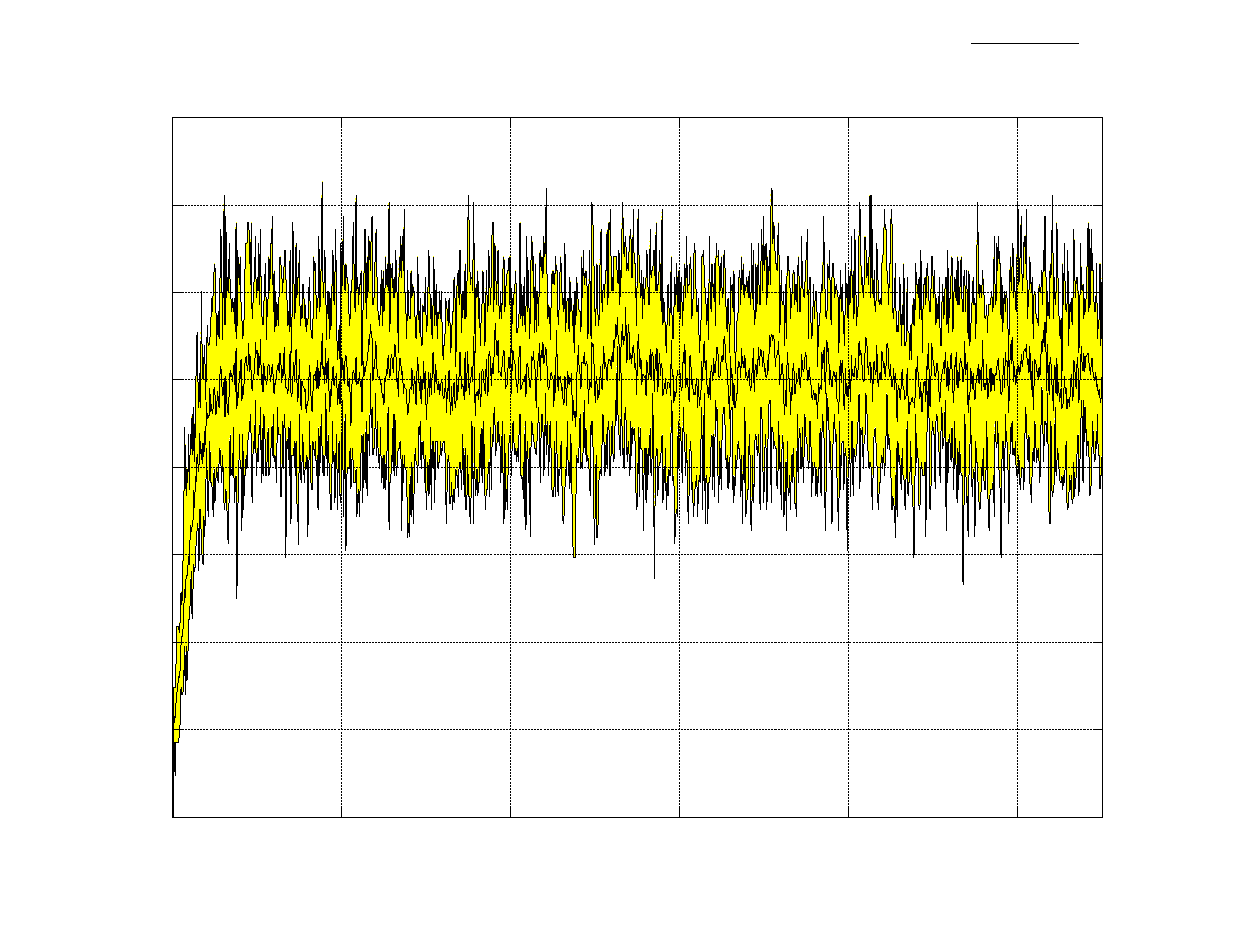
\includegraphics{./images/artificial/gmlaslcs0/identityCex.eps}}%
    \gplfronttext
  \end{picture}%
\endgroup
}
  \put(-285,70){\rotatebox{90}{$Exact \: Match$}}
  \scalebox{0.8}{\put(-200,0){\rotatebox{0}{$iterations$}}}
  \label{fig:gmlaslcs0Cidentity7Ex}  
   
  \centering
  \scalebox{0.49}{\Large% GNUPLOT: LaTeX picture with Postscript
\begingroup
  \makeatletter
  \providecommand\color[2][]{%
    \GenericError{(gnuplot) \space\space\space\@spaces}{%
      Package color not loaded in conjunction with
      terminal option `colourtext'%
    }{See the gnuplot documentation for explanation.%
    }{Either use 'blacktext' in gnuplot or load the package
      color.sty in LaTeX.}%
    \renewcommand\color[2][]{}%
  }%
  \providecommand\includegraphics[2][]{%
    \GenericError{(gnuplot) \space\space\space\@spaces}{%
      Package graphicx or graphics not loaded%
    }{See the gnuplot documentation for explanation.%
    }{The gnuplot epslatex terminal needs graphicx.sty or graphics.sty.}%
    \renewcommand\includegraphics[2][]{}%
  }%
  \providecommand\rotatebox[2]{#2}%
  \@ifundefined{ifGPcolor}{%
    \newif\ifGPcolor
    \GPcolorfalse
  }{}%
  \@ifundefined{ifGPblacktext}{%
    \newif\ifGPblacktext
    \GPblacktexttrue
  }{}%
  % define a \g@addto@macro without @ in the name:
  \let\gplgaddtomacro\g@addto@macro
  % define empty templates for all commands taking text:
  \gdef\gplbacktext{}%
  \gdef\gplfronttext{}%
  \makeatother
  \ifGPblacktext
    % no textcolor at all
    \def\colorrgb#1{}%
    \def\colorgray#1{}%
  \else
    % gray or color?
    \ifGPcolor
      \def\colorrgb#1{\color[rgb]{#1}}%
      \def\colorgray#1{\color[gray]{#1}}%
      \expandafter\def\csname LTw\endcsname{\color{white}}%
      \expandafter\def\csname LTb\endcsname{\color{black}}%
      \expandafter\def\csname LTa\endcsname{\color{black}}%
      \expandafter\def\csname LT0\endcsname{\color[rgb]{1,0,0}}%
      \expandafter\def\csname LT1\endcsname{\color[rgb]{0,1,0}}%
      \expandafter\def\csname LT2\endcsname{\color[rgb]{0,0,1}}%
      \expandafter\def\csname LT3\endcsname{\color[rgb]{1,0,1}}%
      \expandafter\def\csname LT4\endcsname{\color[rgb]{0,1,1}}%
      \expandafter\def\csname LT5\endcsname{\color[rgb]{1,1,0}}%
      \expandafter\def\csname LT6\endcsname{\color[rgb]{0,0,0}}%
      \expandafter\def\csname LT7\endcsname{\color[rgb]{1,0.3,0}}%
      \expandafter\def\csname LT8\endcsname{\color[rgb]{0.5,0.5,0.5}}%
    \else
      % gray
      \def\colorrgb#1{\color{black}}%
      \def\colorgray#1{\color[gray]{#1}}%
      \expandafter\def\csname LTw\endcsname{\color{white}}%
      \expandafter\def\csname LTb\endcsname{\color{black}}%
      \expandafter\def\csname LTa\endcsname{\color{black}}%
      \expandafter\def\csname LT0\endcsname{\color{black}}%
      \expandafter\def\csname LT1\endcsname{\color{black}}%
      \expandafter\def\csname LT2\endcsname{\color{black}}%
      \expandafter\def\csname LT3\endcsname{\color{black}}%
      \expandafter\def\csname LT4\endcsname{\color{black}}%
      \expandafter\def\csname LT5\endcsname{\color{black}}%
      \expandafter\def\csname LT6\endcsname{\color{black}}%
      \expandafter\def\csname LT7\endcsname{\color{black}}%
      \expandafter\def\csname LT8\endcsname{\color{black}}%
    \fi
  \fi
  \setlength{\unitlength}{0.0500bp}%
  \begin{picture}(11520.00,8640.00)%
    \gplgaddtomacro\gplbacktext{%
    }%
    \gplgaddtomacro\gplfronttext{%
      \csname LTb\endcsname%
      \put(9049,8377){\makebox(0,0)[r]{\strut{}$GMl-ASLCS_{\:0C} \: mean \: BAM \: coverage \: in  \:mlIdentity_7$}}%
      \colorrgb{0.00,0.00,0.00}%
      \put(1257,950){\makebox(0,0)[r]{\strut{}$0$}}%
      \colorrgb{0.00,0.00,0.00}%
      \put(1257,2294){\makebox(0,0)[r]{\strut{}$0.05$}}%
      \colorrgb{0.00,0.00,0.00}%
      \put(1257,3637){\makebox(0,0)[r]{\strut{}$0.1$}}%
      \colorrgb{0.00,0.00,0.00}%
      \put(1257,4981){\makebox(0,0)[r]{\strut{}$0.15$}}%
      \colorrgb{0.00,0.00,0.00}%
      \put(1257,6324){\makebox(0,0)[r]{\strut{}$0.2$}}%
      \colorrgb{0.00,0.00,0.00}%
      \put(1257,7668){\makebox(0,0)[r]{\strut{}$0.25$}}%
      \colorrgb{0.00,0.00,0.00}%
      \put(1497,550){\makebox(0,0){\strut{}$0$}}%
      \colorrgb{0.00,0.00,0.00}%
      \put(3120,550){\makebox(0,0){\strut{}$200$}}%
      \colorrgb{0.00,0.00,0.00}%
      \put(4743,550){\makebox(0,0){\strut{}$400$}}%
      \colorrgb{0.00,0.00,0.00}%
      \put(6366,550){\makebox(0,0){\strut{}$600$}}%
      \colorrgb{0.00,0.00,0.00}%
      \put(7989,550){\makebox(0,0){\strut{}$800$}}%
      \colorrgb{0.00,0.00,0.00}%
      \put(9612,550){\makebox(0,0){\strut{}$1000$}}%
    }%
    \gplbacktext
    \put(0,0){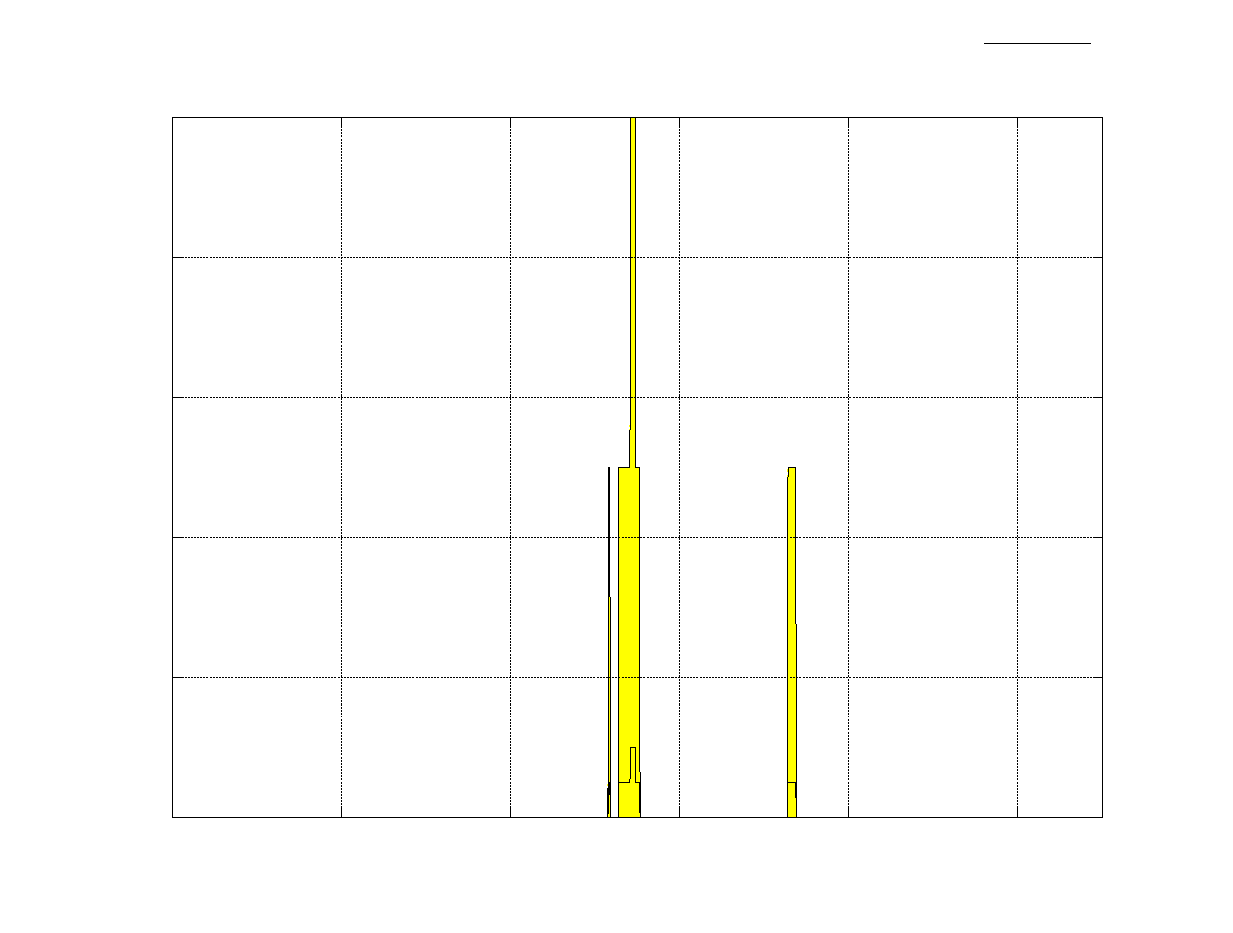
\includegraphics{./images/artificial/gmlaslcs0/identityCBAM.eps}}%
    \gplfronttext
  \end{picture}%
\endgroup
}
  \put(-285,80){\rotatebox{90}{$BAM$}}
  \scalebox{0.8}{\put(-200,0){\rotatebox{0}{$iterations$}}}
  \label{fig:gmlaslcs0Cidentity7BAM} 
\end{figure}

Οι GMl-ASLCS$_{\:0D}$ και GMl-ASLCS$_{\:0GA}$ κινούνται στα ίδια πλαίσια με τον GMl-ASLCS$_{\:0}$ ως προς τις τελικες τιμές των μετρικών αξιολόγησης, αλλά καταφέρνουν να συγκλίνουν γρηγορότερα, μειώνοντας ταυτόχρονα το εύρος τους. Όσον αφορά στην εύρεση του Βέλτιστου Χάρτη, παρατηρούμε πως και εδώ κινούνται στα βήματα του GMl-ASLCS$_{\:0}$, αλλά μέσω του μπορούμε να βγάλουμε το συμπέρασμα πως καταφέρνουν να γενικεύσουν καλύτερα από τον GMl-ASLCS$_{\:0}$ (αλλά χειρότερα από όσο στο σύνολο $mlPosition_{7}$, ίσως λόγω και της μεγαλύτερης πολυκατηγορικής πληθικότητας του συνόλου $mlIdentity_{7}$). Συνεπώς, και εδώ οι τροποποιήσεις της λειτουργίας διαγραφής και του τελεστή διασταύρωσης επιτυγχάνουν να διατηρήσουν την Ακρίβεια του τελικού μοντέλου που αναπτύσσουν, με ταυτόχρονη αύξηση του αριθμού δειγμάτων που καλύπτουν οι κανόνες τους. 

Ο GMl-ASLCS$_{\:0M}$, εδώ, καταφέρνει να κάνει παρατηρήσιμη τη λειτουργία για την οποία επινοήσαμε τη διαγραφή κανόνων από τα Match Sets. Εκμεταλλευόμενος την ισοτροπία διαχείρισης των αδιαφοριών στο τμήμα της απόφασης των κανόνων από τη συνιστώσα ενημέρωσης και την ύπαρξη πληθώρας αδιαφοριών για ετικέτες από τους κανόνες του βέλτιστου χάρτη για το σύνολο $mlIdentity_{7}$, καταφέρνει να αυξήσει τη μέση κάλυψη των κανόνων του πληθυμού, καταλήγοντας σε μία αύξηση κατά $10\%$ του ποσοστού εύρεσης του βέλτιστου χάρτη, διατηρώντας ταυτόχρονα τις μετρικές της Ακρίβειας και της Ακριβούς Ορθότητας στα ίδια επίπεδα με αυτά του GMl-ASLCS$_{\:0}$ για το ίδιο πρόβλημα.
% Παρατηρούμε και εδώ, όχι μόνο τη σύγκλιση στις σχεδόν βέλτιστες λύσεις, αλλά και το γεγονός πως αυτές επιτυγχάνονται κοντά στις $400$ επαναλήψεις, σε αντιδιαστολή με τον GMl-ASLCS$_{\:0}$ που στο τέλος των $1000$ επαναλήψεων δεν τις έχει επιτύχει.

Λόγω της ισχυρής παρουσίας αδιαφοριών στις ετικέτες των κανόνων του Χάρτη Βέλτιστων Αποφάσεων και της τιμωρίας κανόνων που αδιαφορούν για ετικέτες μέσω της έκπτωσης της καταλληλότητας τους, ο GMl-ASLCS$_{\:0C}$ αποτυγχάνει πλήρως να αναπτύξει το Βέλτιστο Χάρτη. Ωστόσο, η ανάπτυξή του, όπως προαναφέραμε, είναι μία ικανή και όχι αναγκαία συνθήκη, και για αυτό δεν μπορούμε να συμπεράνουμε κάτι παραπάνω για τη συμπεριφορά του GMl-ASLCS$_{\:0C}$. Από τα γραφήματα της Ακρίβειας και της Ακριβούς Ορθότητας, όμως, παρατηρούμε την αδυναμία του GMl-ASLCS$_{\:0C}$ να εμφανίσει μία αύξουσα πορεία ως προς αυτές και, συνεπώς, την αδυναμία εύρεσης νέων, βελτιωμένων συνολικά λύσεων στο πολυκατηγορικό πρόβλημα. Η αδυναμία αυτή πηγάζει κυρίως από τη Διασταύρωση Ενός Σημείου που χρησιμοποιεί ο Γενετικός Αλγόριθμος του GMl-ASLCS$_{\:0}$ και ενισχύεται από την υψηλή κατηγορική πληθικότητα του συνόλου δεδομένων $mlIdentity_{7}$. 


%-----------------------------------------adder7_3-----------------------------------------%



\subsection{Οι τροποποιημένοι αλγόριθμοι GMl-ASLCS$_{\:0*}$ στο πρόβλημα $adder_{7}^{3}$}
Τα Σχήματα \ref{fig:gmlaslcs0Dadder7_3}, \ref{fig:gmlaslcs0GAadder7_3}, \ref{fig:gmlaslcs0Madder7_3} και \ref{fig:gmlaslcs0Cadder7_3} παρουσιάζουν την εξέλιξη των μετρικών της Ακρίβειας και της Ακριβούς Ορθότητας για το σύνολο δεδομένων  $adder_{7}^{3}$, των ΜαΣΤ GMl-ASLCS$_{\:0D}$, GMl-ASLCS$_{\:0GA}$, GMl-ASLCS$_{\:0M}$ και GMl-ASLCS$_{\:0C}$, αντίστοιχα.


Οι GMl-ASLCS$_{\:0D}$ και GMl-ASLCS$_{\:0GA}$ καταφέρνουν και εδώ να βρουν γρηγορότερα το τελικό σύνολο λύσεων (δηλαδή τους κανόνες του ΧΒΑ), με ταυτόχρονη αύξηση της τελικής Ακριβούς Ορθότητας, και αύξηση της Ακρίβειας για τον GMl-ASLCS$_{\:0GA}$. Ωστόσο, ο GMl-ASLCS$_{\:0GA}$ φαίνεται ότι είναι εξαιρετικά συνεπής, καθώς μειώνει αισθητά το εύρος των μετρικών αξιολόγησης, περισσότερο από τον GMl-ASLCS$_{\:0D}$. Ένα σημείο ανησυχίας παρατηρείται στο διάστημα των τελευταίων επαναλήψεων, όπου το εύρος της Ακρίβειας και ακόμη περισσότερο της Ακριβούς Ορθότητας φαίνεται ότι αυξάνεται, φανερώνοντας πιθανά συμπτώματα υπερεκπαίδευσης. 

Ο GMl-ASLCS$_{\:0M}$ εμφανίζει ελαφρώς αυξημένα επίπεδα τιμών Ακρίβειας και σημαντικά αυξημένα επίπεδα Ακριβούς Ορθότητας, ενώ καταφέρνει να μειώσει τις ελάχιστες τιμές τους, ιδιαίτερα στις τελευταίες επαναλήψεις, σε αντίθεση με τον GMl-ASLCS$_{\:0}$. Το ποσοστό κάλυψης, αν και δε φαίνεται στα διαγράμματα, αυξάνει και αυτό και μάλιστα διπλασιάζεται.

Ο GMl-ASLCS$_{\:0C}$ εμφανίζει και εδώ το πρόβλημα της στασιμότητας των λύσεων που αναπτύσσει, όπως και στο πρόβλημα $mlIdentity_{7}$. Επιπλέον, και εδώ εντοπίζουμε την ίδια συμπεριφορά του Γενετικού Αλγορίθμου, καθώς τα δύο σύνολα διαθέτουν την ίδια τιμή πολυκατηγορικής πληθικότητας.

\begin{figure}[ht]
  \caption{Διαγράμματα χαρτογράφησης $adder_{7}^{3}$ του GMl-ASLCS$_{\:0D}$.}
  \label{fig:gmlaslcs0Dadder7_3}
  \begin{minipage}[b]{0.5\linewidth}
  	\centering
  	\scalebox{0.42}{\Large% GNUPLOT: LaTeX picture with Postscript
\begingroup
  \makeatletter
  \providecommand\color[2][]{%
    \GenericError{(gnuplot) \space\space\space\@spaces}{%
      Package color not loaded in conjunction with
      terminal option `colourtext'%
    }{See the gnuplot documentation for explanation.%
    }{Either use 'blacktext' in gnuplot or load the package
      color.sty in LaTeX.}%
    \renewcommand\color[2][]{}%
  }%
  \providecommand\includegraphics[2][]{%
    \GenericError{(gnuplot) \space\space\space\@spaces}{%
      Package graphicx or graphics not loaded%
    }{See the gnuplot documentation for explanation.%
    }{The gnuplot epslatex terminal needs graphicx.sty or graphics.sty.}%
    \renewcommand\includegraphics[2][]{}%
  }%
  \providecommand\rotatebox[2]{#2}%
  \@ifundefined{ifGPcolor}{%
    \newif\ifGPcolor
    \GPcolorfalse
  }{}%
  \@ifundefined{ifGPblacktext}{%
    \newif\ifGPblacktext
    \GPblacktexttrue
  }{}%
  % define a \g@addto@macro without @ in the name:
  \let\gplgaddtomacro\g@addto@macro
  % define empty templates for all commands taking text:
  \gdef\gplbacktext{}%
  \gdef\gplfronttext{}%
  \makeatother
  \ifGPblacktext
    % no textcolor at all
    \def\colorrgb#1{}%
    \def\colorgray#1{}%
  \else
    % gray or color?
    \ifGPcolor
      \def\colorrgb#1{\color[rgb]{#1}}%
      \def\colorgray#1{\color[gray]{#1}}%
      \expandafter\def\csname LTw\endcsname{\color{white}}%
      \expandafter\def\csname LTb\endcsname{\color{black}}%
      \expandafter\def\csname LTa\endcsname{\color{black}}%
      \expandafter\def\csname LT0\endcsname{\color[rgb]{1,0,0}}%
      \expandafter\def\csname LT1\endcsname{\color[rgb]{0,1,0}}%
      \expandafter\def\csname LT2\endcsname{\color[rgb]{0,0,1}}%
      \expandafter\def\csname LT3\endcsname{\color[rgb]{1,0,1}}%
      \expandafter\def\csname LT4\endcsname{\color[rgb]{0,1,1}}%
      \expandafter\def\csname LT5\endcsname{\color[rgb]{1,1,0}}%
      \expandafter\def\csname LT6\endcsname{\color[rgb]{0,0,0}}%
      \expandafter\def\csname LT7\endcsname{\color[rgb]{1,0.3,0}}%
      \expandafter\def\csname LT8\endcsname{\color[rgb]{0.5,0.5,0.5}}%
    \else
      % gray
      \def\colorrgb#1{\color{black}}%
      \def\colorgray#1{\color[gray]{#1}}%
      \expandafter\def\csname LTw\endcsname{\color{white}}%
      \expandafter\def\csname LTb\endcsname{\color{black}}%
      \expandafter\def\csname LTa\endcsname{\color{black}}%
      \expandafter\def\csname LT0\endcsname{\color{black}}%
      \expandafter\def\csname LT1\endcsname{\color{black}}%
      \expandafter\def\csname LT2\endcsname{\color{black}}%
      \expandafter\def\csname LT3\endcsname{\color{black}}%
      \expandafter\def\csname LT4\endcsname{\color{black}}%
      \expandafter\def\csname LT5\endcsname{\color{black}}%
      \expandafter\def\csname LT6\endcsname{\color{black}}%
      \expandafter\def\csname LT7\endcsname{\color{black}}%
      \expandafter\def\csname LT8\endcsname{\color{black}}%
    \fi
  \fi
  \setlength{\unitlength}{0.0500bp}%
  \begin{picture}(11520.00,8640.00)%
    \gplgaddtomacro\gplbacktext{%
    }%
    \gplgaddtomacro\gplfronttext{%
      \csname LTb\endcsname%
      \put(8209,8377){\makebox(0,0)[r]{\strut{}$GMl-ASLCS_{\:0D} \: mean  \:accuracy  \:in  \:adder_7^3$}}%
      \colorrgb{0.00,0.00,0.00}%
      \put(1257,950){\makebox(0,0)[r]{\strut{}$0$}}%
      \colorrgb{0.00,0.00,0.00}%
      \put(1257,2294){\makebox(0,0)[r]{\strut{}$0.2$}}%
      \colorrgb{0.00,0.00,0.00}%
      \put(1257,3637){\makebox(0,0)[r]{\strut{}$0.4$}}%
      \colorrgb{0.00,0.00,0.00}%
      \put(1257,4981){\makebox(0,0)[r]{\strut{}$0.6$}}%
      \colorrgb{0.00,0.00,0.00}%
      \put(1257,6324){\makebox(0,0)[r]{\strut{}$0.8$}}%
      \colorrgb{0.00,0.00,0.00}%
      \put(1257,7668){\makebox(0,0)[r]{\strut{}$1$}}%
      \colorrgb{0.00,0.00,0.00}%
      \put(1497,550){\makebox(0,0){\strut{}$0$}}%
      \colorrgb{0.00,0.00,0.00}%
      \put(3120,550){\makebox(0,0){\strut{}$200$}}%
      \colorrgb{0.00,0.00,0.00}%
      \put(4743,550){\makebox(0,0){\strut{}$400$}}%
      \colorrgb{0.00,0.00,0.00}%
      \put(6366,550){\makebox(0,0){\strut{}$600$}}%
      \colorrgb{0.00,0.00,0.00}%
      \put(7989,550){\makebox(0,0){\strut{}$800$}}%
      \colorrgb{0.00,0.00,0.00}%
      \put(9612,550){\makebox(0,0){\strut{}$1000$}}%
    }%
    \gplbacktext
    \put(0,0){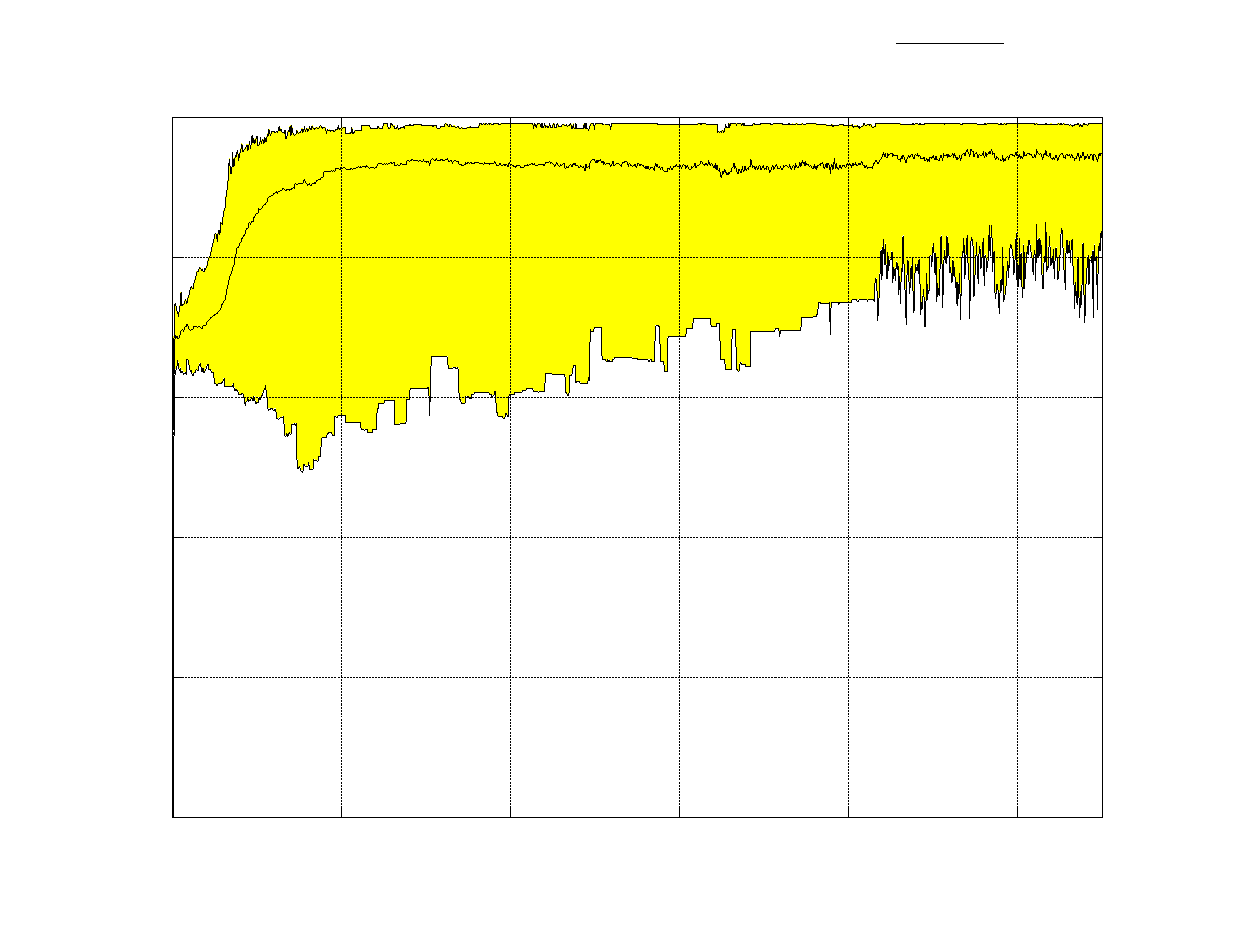
\includegraphics{./images/artificial/gmlaslcs0/adder7_3Dacc.eps}}%
    \gplfronttext
  \end{picture}%
\endgroup
}
  	\put(-240,60){\rotatebox{90}{$Accuracy$}}
 	\scalebox{0.8}{\put(-180,0){\rotatebox{0}{$iterations$}}}  
  	\end{minipage}
  \begin{minipage}[b]{0.5\linewidth}
  	\centering
  	\scalebox{0.42}{\Large% GNUPLOT: LaTeX picture with Postscript
\begingroup
  \makeatletter
  \providecommand\color[2][]{%
    \GenericError{(gnuplot) \space\space\space\@spaces}{%
      Package color not loaded in conjunction with
      terminal option `colourtext'%
    }{See the gnuplot documentation for explanation.%
    }{Either use 'blacktext' in gnuplot or load the package
      color.sty in LaTeX.}%
    \renewcommand\color[2][]{}%
  }%
  \providecommand\includegraphics[2][]{%
    \GenericError{(gnuplot) \space\space\space\@spaces}{%
      Package graphicx or graphics not loaded%
    }{See the gnuplot documentation for explanation.%
    }{The gnuplot epslatex terminal needs graphicx.sty or graphics.sty.}%
    \renewcommand\includegraphics[2][]{}%
  }%
  \providecommand\rotatebox[2]{#2}%
  \@ifundefined{ifGPcolor}{%
    \newif\ifGPcolor
    \GPcolorfalse
  }{}%
  \@ifundefined{ifGPblacktext}{%
    \newif\ifGPblacktext
    \GPblacktexttrue
  }{}%
  % define a \g@addto@macro without @ in the name:
  \let\gplgaddtomacro\g@addto@macro
  % define empty templates for all commands taking text:
  \gdef\gplbacktext{}%
  \gdef\gplfronttext{}%
  \makeatother
  \ifGPblacktext
    % no textcolor at all
    \def\colorrgb#1{}%
    \def\colorgray#1{}%
  \else
    % gray or color?
    \ifGPcolor
      \def\colorrgb#1{\color[rgb]{#1}}%
      \def\colorgray#1{\color[gray]{#1}}%
      \expandafter\def\csname LTw\endcsname{\color{white}}%
      \expandafter\def\csname LTb\endcsname{\color{black}}%
      \expandafter\def\csname LTa\endcsname{\color{black}}%
      \expandafter\def\csname LT0\endcsname{\color[rgb]{1,0,0}}%
      \expandafter\def\csname LT1\endcsname{\color[rgb]{0,1,0}}%
      \expandafter\def\csname LT2\endcsname{\color[rgb]{0,0,1}}%
      \expandafter\def\csname LT3\endcsname{\color[rgb]{1,0,1}}%
      \expandafter\def\csname LT4\endcsname{\color[rgb]{0,1,1}}%
      \expandafter\def\csname LT5\endcsname{\color[rgb]{1,1,0}}%
      \expandafter\def\csname LT6\endcsname{\color[rgb]{0,0,0}}%
      \expandafter\def\csname LT7\endcsname{\color[rgb]{1,0.3,0}}%
      \expandafter\def\csname LT8\endcsname{\color[rgb]{0.5,0.5,0.5}}%
    \else
      % gray
      \def\colorrgb#1{\color{black}}%
      \def\colorgray#1{\color[gray]{#1}}%
      \expandafter\def\csname LTw\endcsname{\color{white}}%
      \expandafter\def\csname LTb\endcsname{\color{black}}%
      \expandafter\def\csname LTa\endcsname{\color{black}}%
      \expandafter\def\csname LT0\endcsname{\color{black}}%
      \expandafter\def\csname LT1\endcsname{\color{black}}%
      \expandafter\def\csname LT2\endcsname{\color{black}}%
      \expandafter\def\csname LT3\endcsname{\color{black}}%
      \expandafter\def\csname LT4\endcsname{\color{black}}%
      \expandafter\def\csname LT5\endcsname{\color{black}}%
      \expandafter\def\csname LT6\endcsname{\color{black}}%
      \expandafter\def\csname LT7\endcsname{\color{black}}%
      \expandafter\def\csname LT8\endcsname{\color{black}}%
    \fi
  \fi
  \setlength{\unitlength}{0.0500bp}%
  \begin{picture}(11520.00,8640.00)%
    \gplgaddtomacro\gplbacktext{%
    }%
    \gplgaddtomacro\gplfronttext{%
      \csname LTb\endcsname%
      \put(8569,8377){\makebox(0,0)[r]{\strut{}$GMl-ASLCS_{\:0D} \: mean \: exact \: match \: in \: adder_7^3$}}%
      \colorrgb{0.00,0.00,0.00}%
      \put(1257,950){\makebox(0,0)[r]{\strut{}$0$}}%
      \colorrgb{0.00,0.00,0.00}%
      \put(1257,2294){\makebox(0,0)[r]{\strut{}$0.2$}}%
      \colorrgb{0.00,0.00,0.00}%
      \put(1257,3637){\makebox(0,0)[r]{\strut{}$0.4$}}%
      \colorrgb{0.00,0.00,0.00}%
      \put(1257,4981){\makebox(0,0)[r]{\strut{}$0.6$}}%
      \colorrgb{0.00,0.00,0.00}%
      \put(1257,6324){\makebox(0,0)[r]{\strut{}$0.8$}}%
      \colorrgb{0.00,0.00,0.00}%
      \put(1257,7668){\makebox(0,0)[r]{\strut{}$1$}}%
      \colorrgb{0.00,0.00,0.00}%
      \put(1497,550){\makebox(0,0){\strut{}$0$}}%
      \colorrgb{0.00,0.00,0.00}%
      \put(3120,550){\makebox(0,0){\strut{}$200$}}%
      \colorrgb{0.00,0.00,0.00}%
      \put(4743,550){\makebox(0,0){\strut{}$400$}}%
      \colorrgb{0.00,0.00,0.00}%
      \put(6366,550){\makebox(0,0){\strut{}$600$}}%
      \colorrgb{0.00,0.00,0.00}%
      \put(7989,550){\makebox(0,0){\strut{}$800$}}%
      \colorrgb{0.00,0.00,0.00}%
      \put(9612,550){\makebox(0,0){\strut{}$1000$}}%
    }%
    \gplbacktext
    \put(0,0){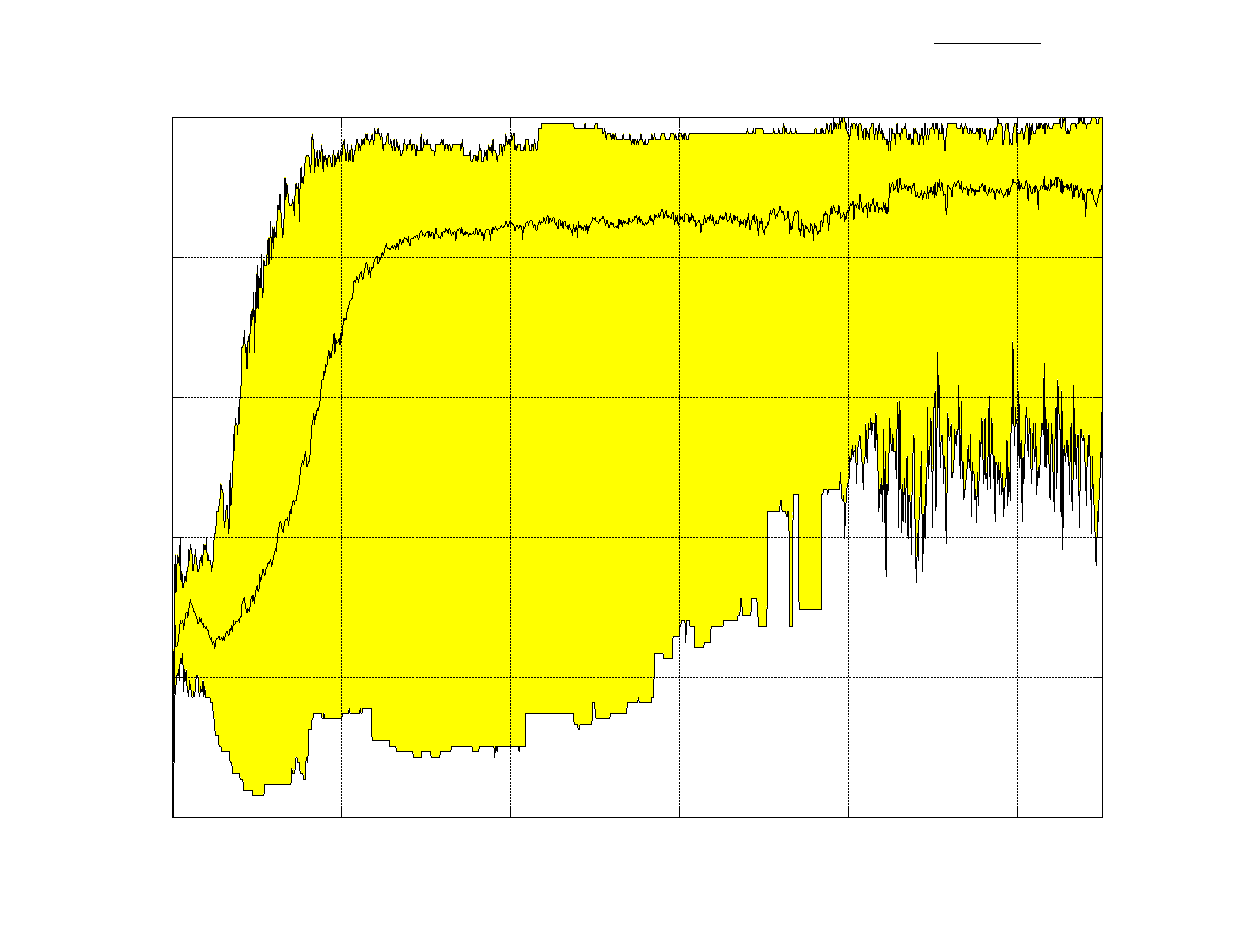
\includegraphics{./images/artificial/gmlaslcs0/adder7_3Mex.eps}}%
    \gplfronttext
  \end{picture}%
\endgroup
}
  	\put(-240,60){\rotatebox{90}{$Exact \: Match$}}
  	\scalebox{0.8}{\put(-180,0){\rotatebox{0}{$iterations$}}}  
  \end{minipage}
\end{figure}

\begin{figure}[ht]
  \caption{Διαγράμματα χαρτογράφησης $adder_{7}^{3}$ του GMl-ASLCS$_{\:0GA}$.}
  \label{fig:gmlaslcs0GAadder7_3}
  \begin{minipage}[b]{0.5\linewidth}
  	\centering
  	\scalebox{0.42}{\Large% GNUPLOT: LaTeX picture with Postscript
\begingroup
  \makeatletter
  \providecommand\color[2][]{%
    \GenericError{(gnuplot) \space\space\space\@spaces}{%
      Package color not loaded in conjunction with
      terminal option `colourtext'%
    }{See the gnuplot documentation for explanation.%
    }{Either use 'blacktext' in gnuplot or load the package
      color.sty in LaTeX.}%
    \renewcommand\color[2][]{}%
  }%
  \providecommand\includegraphics[2][]{%
    \GenericError{(gnuplot) \space\space\space\@spaces}{%
      Package graphicx or graphics not loaded%
    }{See the gnuplot documentation for explanation.%
    }{The gnuplot epslatex terminal needs graphicx.sty or graphics.sty.}%
    \renewcommand\includegraphics[2][]{}%
  }%
  \providecommand\rotatebox[2]{#2}%
  \@ifundefined{ifGPcolor}{%
    \newif\ifGPcolor
    \GPcolorfalse
  }{}%
  \@ifundefined{ifGPblacktext}{%
    \newif\ifGPblacktext
    \GPblacktexttrue
  }{}%
  % define a \g@addto@macro without @ in the name:
  \let\gplgaddtomacro\g@addto@macro
  % define empty templates for all commands taking text:
  \gdef\gplbacktext{}%
  \gdef\gplfronttext{}%
  \makeatother
  \ifGPblacktext
    % no textcolor at all
    \def\colorrgb#1{}%
    \def\colorgray#1{}%
  \else
    % gray or color?
    \ifGPcolor
      \def\colorrgb#1{\color[rgb]{#1}}%
      \def\colorgray#1{\color[gray]{#1}}%
      \expandafter\def\csname LTw\endcsname{\color{white}}%
      \expandafter\def\csname LTb\endcsname{\color{black}}%
      \expandafter\def\csname LTa\endcsname{\color{black}}%
      \expandafter\def\csname LT0\endcsname{\color[rgb]{1,0,0}}%
      \expandafter\def\csname LT1\endcsname{\color[rgb]{0,1,0}}%
      \expandafter\def\csname LT2\endcsname{\color[rgb]{0,0,1}}%
      \expandafter\def\csname LT3\endcsname{\color[rgb]{1,0,1}}%
      \expandafter\def\csname LT4\endcsname{\color[rgb]{0,1,1}}%
      \expandafter\def\csname LT5\endcsname{\color[rgb]{1,1,0}}%
      \expandafter\def\csname LT6\endcsname{\color[rgb]{0,0,0}}%
      \expandafter\def\csname LT7\endcsname{\color[rgb]{1,0.3,0}}%
      \expandafter\def\csname LT8\endcsname{\color[rgb]{0.5,0.5,0.5}}%
    \else
      % gray
      \def\colorrgb#1{\color{black}}%
      \def\colorgray#1{\color[gray]{#1}}%
      \expandafter\def\csname LTw\endcsname{\color{white}}%
      \expandafter\def\csname LTb\endcsname{\color{black}}%
      \expandafter\def\csname LTa\endcsname{\color{black}}%
      \expandafter\def\csname LT0\endcsname{\color{black}}%
      \expandafter\def\csname LT1\endcsname{\color{black}}%
      \expandafter\def\csname LT2\endcsname{\color{black}}%
      \expandafter\def\csname LT3\endcsname{\color{black}}%
      \expandafter\def\csname LT4\endcsname{\color{black}}%
      \expandafter\def\csname LT5\endcsname{\color{black}}%
      \expandafter\def\csname LT6\endcsname{\color{black}}%
      \expandafter\def\csname LT7\endcsname{\color{black}}%
      \expandafter\def\csname LT8\endcsname{\color{black}}%
    \fi
  \fi
  \setlength{\unitlength}{0.0500bp}%
  \begin{picture}(11520.00,8640.00)%
    \gplgaddtomacro\gplbacktext{%
    }%
    \gplgaddtomacro\gplfronttext{%
      \csname LTb\endcsname%
      \put(8209,8377){\makebox(0,0)[r]{\strut{}$GMl-ASLCS_{\:0GA} \: mean \: accuracy  \:in \: adder_7^3$}}%
      \colorrgb{0.00,0.00,0.00}%
      \put(1257,950){\makebox(0,0)[r]{\strut{}$0$}}%
      \colorrgb{0.00,0.00,0.00}%
      \put(1257,2294){\makebox(0,0)[r]{\strut{}$0.2$}}%
      \colorrgb{0.00,0.00,0.00}%
      \put(1257,3637){\makebox(0,0)[r]{\strut{}$0.4$}}%
      \colorrgb{0.00,0.00,0.00}%
      \put(1257,4981){\makebox(0,0)[r]{\strut{}$0.6$}}%
      \colorrgb{0.00,0.00,0.00}%
      \put(1257,6324){\makebox(0,0)[r]{\strut{}$0.8$}}%
      \colorrgb{0.00,0.00,0.00}%
      \put(1257,7668){\makebox(0,0)[r]{\strut{}$1$}}%
      \colorrgb{0.00,0.00,0.00}%
      \put(1497,550){\makebox(0,0){\strut{}$0$}}%
      \colorrgb{0.00,0.00,0.00}%
      \put(3120,550){\makebox(0,0){\strut{}$200$}}%
      \colorrgb{0.00,0.00,0.00}%
      \put(4743,550){\makebox(0,0){\strut{}$400$}}%
      \colorrgb{0.00,0.00,0.00}%
      \put(6366,550){\makebox(0,0){\strut{}$600$}}%
      \colorrgb{0.00,0.00,0.00}%
      \put(7989,550){\makebox(0,0){\strut{}$800$}}%
      \colorrgb{0.00,0.00,0.00}%
      \put(9612,550){\makebox(0,0){\strut{}$1000$}}%
    }%
    \gplbacktext
    \put(0,0){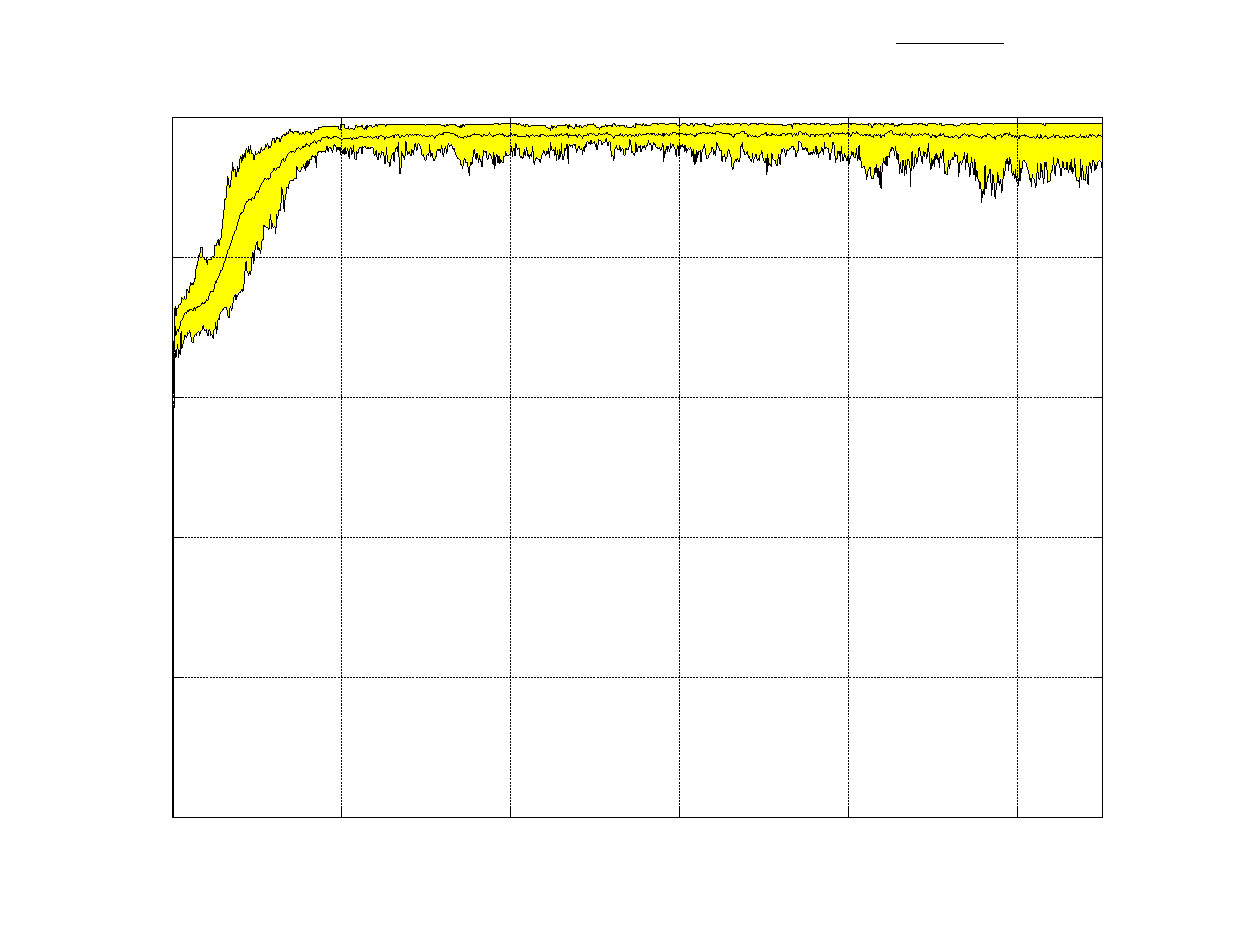
\includegraphics{./images/artificial/gmlaslcs0/adder7_3GAacc.eps}}%
    \gplfronttext
  \end{picture}%
\endgroup
}
  	\put(-240,60){\rotatebox{90}{$Accuracy$}}
 	\scalebox{0.8}{\put(-180,0){\rotatebox{0}{$iterations$}}}  
  	\end{minipage}
  \begin{minipage}[b]{0.5\linewidth}
  	\centering
  	\scalebox{0.42}{\Large% GNUPLOT: LaTeX picture with Postscript
\begingroup
  \makeatletter
  \providecommand\color[2][]{%
    \GenericError{(gnuplot) \space\space\space\@spaces}{%
      Package color not loaded in conjunction with
      terminal option `colourtext'%
    }{See the gnuplot documentation for explanation.%
    }{Either use 'blacktext' in gnuplot or load the package
      color.sty in LaTeX.}%
    \renewcommand\color[2][]{}%
  }%
  \providecommand\includegraphics[2][]{%
    \GenericError{(gnuplot) \space\space\space\@spaces}{%
      Package graphicx or graphics not loaded%
    }{See the gnuplot documentation for explanation.%
    }{The gnuplot epslatex terminal needs graphicx.sty or graphics.sty.}%
    \renewcommand\includegraphics[2][]{}%
  }%
  \providecommand\rotatebox[2]{#2}%
  \@ifundefined{ifGPcolor}{%
    \newif\ifGPcolor
    \GPcolorfalse
  }{}%
  \@ifundefined{ifGPblacktext}{%
    \newif\ifGPblacktext
    \GPblacktexttrue
  }{}%
  % define a \g@addto@macro without @ in the name:
  \let\gplgaddtomacro\g@addto@macro
  % define empty templates for all commands taking text:
  \gdef\gplbacktext{}%
  \gdef\gplfronttext{}%
  \makeatother
  \ifGPblacktext
    % no textcolor at all
    \def\colorrgb#1{}%
    \def\colorgray#1{}%
  \else
    % gray or color?
    \ifGPcolor
      \def\colorrgb#1{\color[rgb]{#1}}%
      \def\colorgray#1{\color[gray]{#1}}%
      \expandafter\def\csname LTw\endcsname{\color{white}}%
      \expandafter\def\csname LTb\endcsname{\color{black}}%
      \expandafter\def\csname LTa\endcsname{\color{black}}%
      \expandafter\def\csname LT0\endcsname{\color[rgb]{1,0,0}}%
      \expandafter\def\csname LT1\endcsname{\color[rgb]{0,1,0}}%
      \expandafter\def\csname LT2\endcsname{\color[rgb]{0,0,1}}%
      \expandafter\def\csname LT3\endcsname{\color[rgb]{1,0,1}}%
      \expandafter\def\csname LT4\endcsname{\color[rgb]{0,1,1}}%
      \expandafter\def\csname LT5\endcsname{\color[rgb]{1,1,0}}%
      \expandafter\def\csname LT6\endcsname{\color[rgb]{0,0,0}}%
      \expandafter\def\csname LT7\endcsname{\color[rgb]{1,0.3,0}}%
      \expandafter\def\csname LT8\endcsname{\color[rgb]{0.5,0.5,0.5}}%
    \else
      % gray
      \def\colorrgb#1{\color{black}}%
      \def\colorgray#1{\color[gray]{#1}}%
      \expandafter\def\csname LTw\endcsname{\color{white}}%
      \expandafter\def\csname LTb\endcsname{\color{black}}%
      \expandafter\def\csname LTa\endcsname{\color{black}}%
      \expandafter\def\csname LT0\endcsname{\color{black}}%
      \expandafter\def\csname LT1\endcsname{\color{black}}%
      \expandafter\def\csname LT2\endcsname{\color{black}}%
      \expandafter\def\csname LT3\endcsname{\color{black}}%
      \expandafter\def\csname LT4\endcsname{\color{black}}%
      \expandafter\def\csname LT5\endcsname{\color{black}}%
      \expandafter\def\csname LT6\endcsname{\color{black}}%
      \expandafter\def\csname LT7\endcsname{\color{black}}%
      \expandafter\def\csname LT8\endcsname{\color{black}}%
    \fi
  \fi
  \setlength{\unitlength}{0.0500bp}%
  \begin{picture}(11520.00,8640.00)%
    \gplgaddtomacro\gplbacktext{%
    }%
    \gplgaddtomacro\gplfronttext{%
      \csname LTb\endcsname%
      \put(8569,8377){\makebox(0,0)[r]{\strut{}$GMl-ASLCS_{\:0GA} \: mean \: exact \: match  \:in  \:adder_7^3$}}%
      \colorrgb{0.00,0.00,0.00}%
      \put(1257,950){\makebox(0,0)[r]{\strut{}$0$}}%
      \colorrgb{0.00,0.00,0.00}%
      \put(1257,2294){\makebox(0,0)[r]{\strut{}$0.2$}}%
      \colorrgb{0.00,0.00,0.00}%
      \put(1257,3637){\makebox(0,0)[r]{\strut{}$0.4$}}%
      \colorrgb{0.00,0.00,0.00}%
      \put(1257,4981){\makebox(0,0)[r]{\strut{}$0.6$}}%
      \colorrgb{0.00,0.00,0.00}%
      \put(1257,6324){\makebox(0,0)[r]{\strut{}$0.8$}}%
      \colorrgb{0.00,0.00,0.00}%
      \put(1257,7668){\makebox(0,0)[r]{\strut{}$1$}}%
      \colorrgb{0.00,0.00,0.00}%
      \put(1497,550){\makebox(0,0){\strut{}$0$}}%
      \colorrgb{0.00,0.00,0.00}%
      \put(3120,550){\makebox(0,0){\strut{}$200$}}%
      \colorrgb{0.00,0.00,0.00}%
      \put(4743,550){\makebox(0,0){\strut{}$400$}}%
      \colorrgb{0.00,0.00,0.00}%
      \put(6366,550){\makebox(0,0){\strut{}$600$}}%
      \colorrgb{0.00,0.00,0.00}%
      \put(7989,550){\makebox(0,0){\strut{}$800$}}%
      \colorrgb{0.00,0.00,0.00}%
      \put(9612,550){\makebox(0,0){\strut{}$1000$}}%
    }%
    \gplbacktext
    \put(0,0){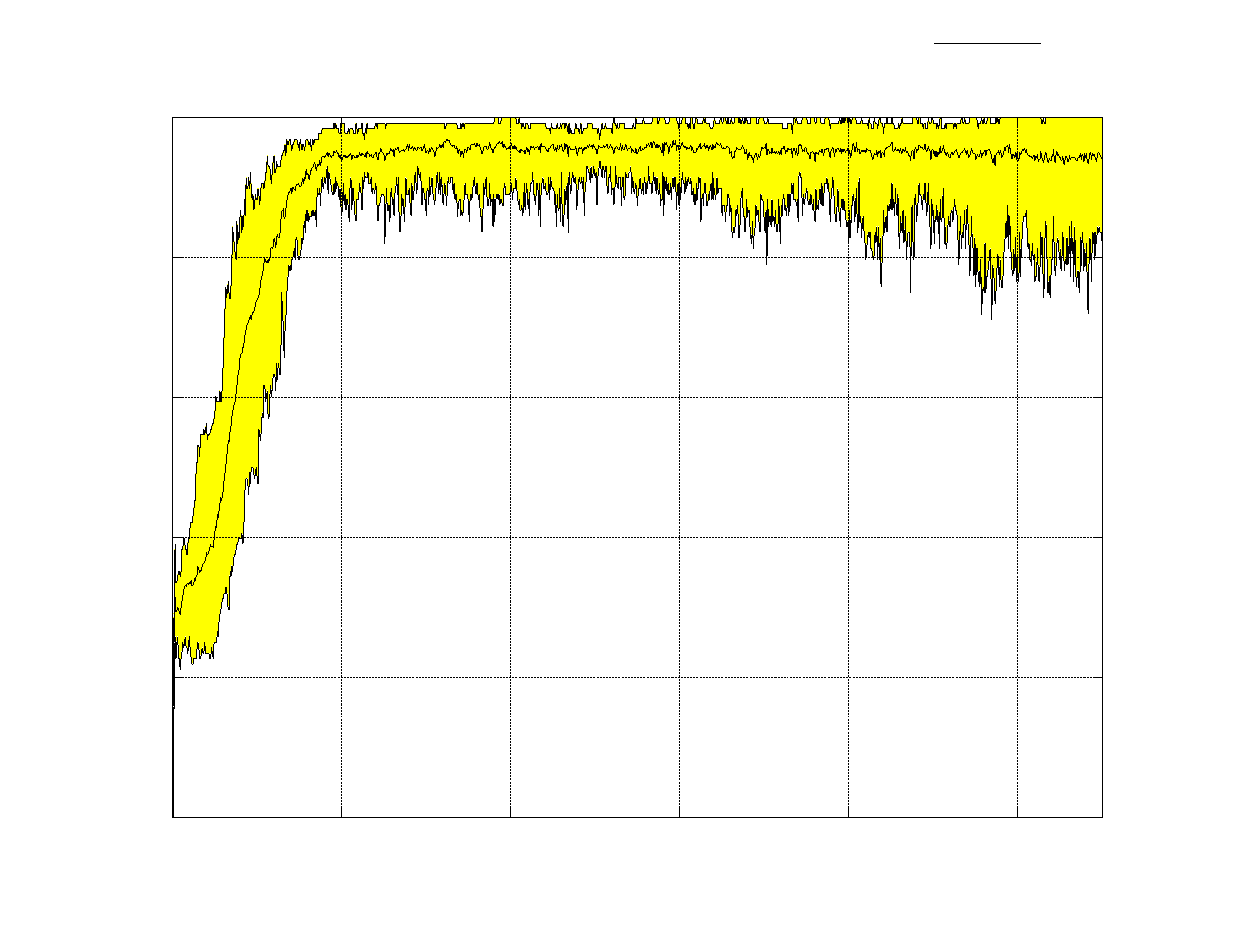
\includegraphics{./images/artificial/gmlaslcs0/adder7_3GAex.eps}}%
    \gplfronttext
  \end{picture}%
\endgroup
}
  	\put(-240,60){\rotatebox{90}{$Exact \: Match$}}
  	\scalebox{0.8}{\put(-180,0){\rotatebox{0}{$iterations$}}}  
  \end{minipage}
\end{figure}

\clearpage


\begin{figure}[ht]
  \caption{Διαγράμματα χαρτογράφησης $adder_{7}^{3}$ του GMl-ASLCS$_{\:0M}$.}
  \label{fig:gmlaslcs0Madder7_3}
  \begin{minipage}[b]{0.5\linewidth}
  	\centering
  	\scalebox{0.42}{\Large% GNUPLOT: LaTeX picture with Postscript
\begingroup
  \makeatletter
  \providecommand\color[2][]{%
    \GenericError{(gnuplot) \space\space\space\@spaces}{%
      Package color not loaded in conjunction with
      terminal option `colourtext'%
    }{See the gnuplot documentation for explanation.%
    }{Either use 'blacktext' in gnuplot or load the package
      color.sty in LaTeX.}%
    \renewcommand\color[2][]{}%
  }%
  \providecommand\includegraphics[2][]{%
    \GenericError{(gnuplot) \space\space\space\@spaces}{%
      Package graphicx or graphics not loaded%
    }{See the gnuplot documentation for explanation.%
    }{The gnuplot epslatex terminal needs graphicx.sty or graphics.sty.}%
    \renewcommand\includegraphics[2][]{}%
  }%
  \providecommand\rotatebox[2]{#2}%
  \@ifundefined{ifGPcolor}{%
    \newif\ifGPcolor
    \GPcolorfalse
  }{}%
  \@ifundefined{ifGPblacktext}{%
    \newif\ifGPblacktext
    \GPblacktexttrue
  }{}%
  % define a \g@addto@macro without @ in the name:
  \let\gplgaddtomacro\g@addto@macro
  % define empty templates for all commands taking text:
  \gdef\gplbacktext{}%
  \gdef\gplfronttext{}%
  \makeatother
  \ifGPblacktext
    % no textcolor at all
    \def\colorrgb#1{}%
    \def\colorgray#1{}%
  \else
    % gray or color?
    \ifGPcolor
      \def\colorrgb#1{\color[rgb]{#1}}%
      \def\colorgray#1{\color[gray]{#1}}%
      \expandafter\def\csname LTw\endcsname{\color{white}}%
      \expandafter\def\csname LTb\endcsname{\color{black}}%
      \expandafter\def\csname LTa\endcsname{\color{black}}%
      \expandafter\def\csname LT0\endcsname{\color[rgb]{1,0,0}}%
      \expandafter\def\csname LT1\endcsname{\color[rgb]{0,1,0}}%
      \expandafter\def\csname LT2\endcsname{\color[rgb]{0,0,1}}%
      \expandafter\def\csname LT3\endcsname{\color[rgb]{1,0,1}}%
      \expandafter\def\csname LT4\endcsname{\color[rgb]{0,1,1}}%
      \expandafter\def\csname LT5\endcsname{\color[rgb]{1,1,0}}%
      \expandafter\def\csname LT6\endcsname{\color[rgb]{0,0,0}}%
      \expandafter\def\csname LT7\endcsname{\color[rgb]{1,0.3,0}}%
      \expandafter\def\csname LT8\endcsname{\color[rgb]{0.5,0.5,0.5}}%
    \else
      % gray
      \def\colorrgb#1{\color{black}}%
      \def\colorgray#1{\color[gray]{#1}}%
      \expandafter\def\csname LTw\endcsname{\color{white}}%
      \expandafter\def\csname LTb\endcsname{\color{black}}%
      \expandafter\def\csname LTa\endcsname{\color{black}}%
      \expandafter\def\csname LT0\endcsname{\color{black}}%
      \expandafter\def\csname LT1\endcsname{\color{black}}%
      \expandafter\def\csname LT2\endcsname{\color{black}}%
      \expandafter\def\csname LT3\endcsname{\color{black}}%
      \expandafter\def\csname LT4\endcsname{\color{black}}%
      \expandafter\def\csname LT5\endcsname{\color{black}}%
      \expandafter\def\csname LT6\endcsname{\color{black}}%
      \expandafter\def\csname LT7\endcsname{\color{black}}%
      \expandafter\def\csname LT8\endcsname{\color{black}}%
    \fi
  \fi
  \setlength{\unitlength}{0.0500bp}%
  \begin{picture}(11520.00,8640.00)%
    \gplgaddtomacro\gplbacktext{%
    }%
    \gplgaddtomacro\gplfronttext{%
      \csname LTb\endcsname%
      \put(8209,8377){\makebox(0,0)[r]{\strut{}$GMl-ASLCS_{\:0M} \: mean \: accuracy \: in \: adder_7^3$}}%
      \colorrgb{0.00,0.00,0.00}%
      \put(1257,950){\makebox(0,0)[r]{\strut{}$0$}}%
      \colorrgb{0.00,0.00,0.00}%
      \put(1257,2294){\makebox(0,0)[r]{\strut{}$0.2$}}%
      \colorrgb{0.00,0.00,0.00}%
      \put(1257,3637){\makebox(0,0)[r]{\strut{}$0.4$}}%
      \colorrgb{0.00,0.00,0.00}%
      \put(1257,4981){\makebox(0,0)[r]{\strut{}$0.6$}}%
      \colorrgb{0.00,0.00,0.00}%
      \put(1257,6324){\makebox(0,0)[r]{\strut{}$0.8$}}%
      \colorrgb{0.00,0.00,0.00}%
      \put(1257,7668){\makebox(0,0)[r]{\strut{}$1$}}%
      \colorrgb{0.00,0.00,0.00}%
      \put(1497,550){\makebox(0,0){\strut{}$0$}}%
      \colorrgb{0.00,0.00,0.00}%
      \put(3120,550){\makebox(0,0){\strut{}$200$}}%
      \colorrgb{0.00,0.00,0.00}%
      \put(4743,550){\makebox(0,0){\strut{}$400$}}%
      \colorrgb{0.00,0.00,0.00}%
      \put(6366,550){\makebox(0,0){\strut{}$600$}}%
      \colorrgb{0.00,0.00,0.00}%
      \put(7989,550){\makebox(0,0){\strut{}$800$}}%
      \colorrgb{0.00,0.00,0.00}%
      \put(9612,550){\makebox(0,0){\strut{}$1000$}}%
    }%
    \gplbacktext
    \put(0,0){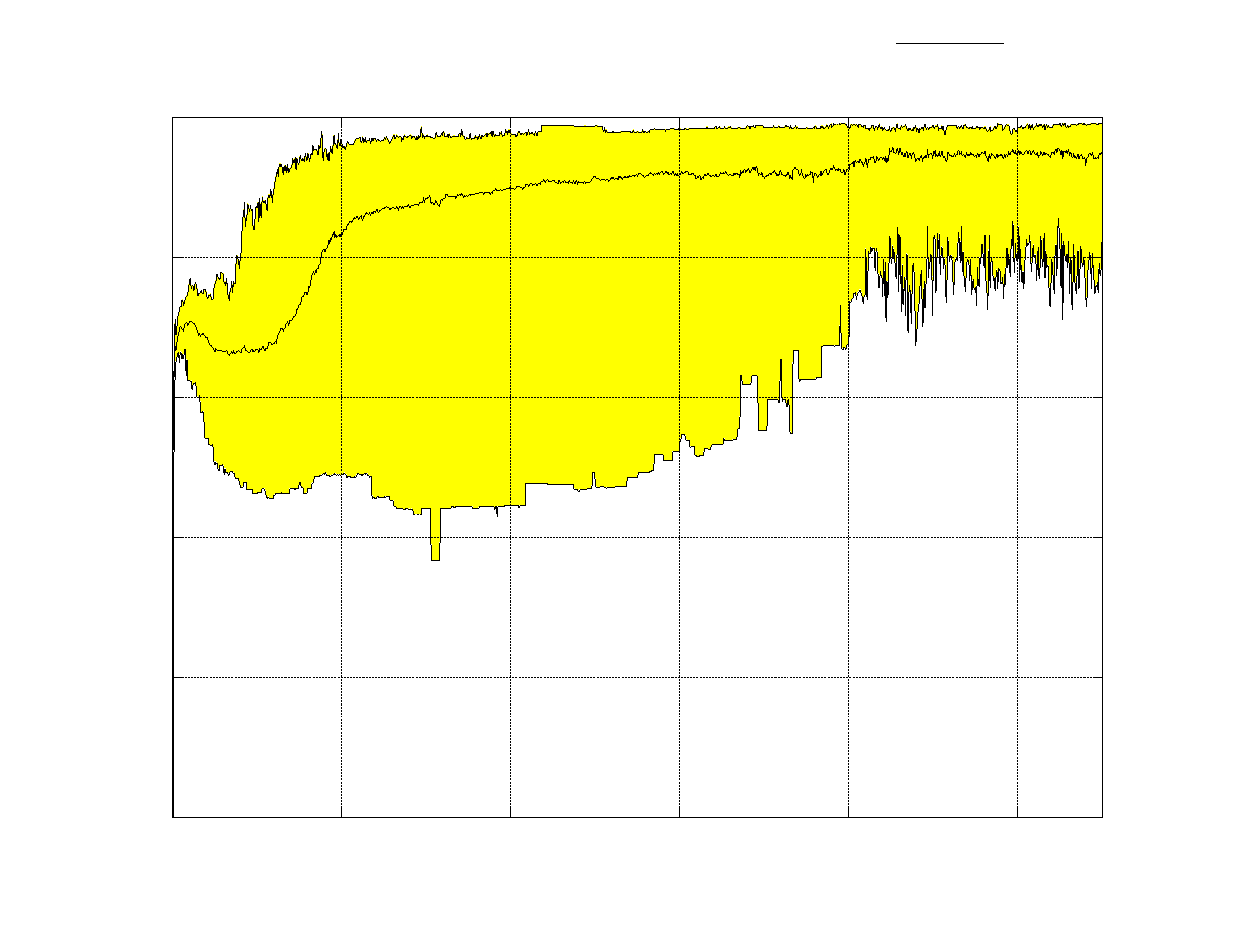
\includegraphics{./images/artificial/gmlaslcs0/adder7_3Macc.eps}}%
    \gplfronttext
  \end{picture}%
\endgroup
}
  	\put(-240,60){\rotatebox{90}{$Accuracy$}}
 	\scalebox{0.8}{\put(-180,0){\rotatebox{0}{$iterations$}}}  
  	\end{minipage}
  \begin{minipage}[b]{0.5\linewidth}
  	\centering
  	\scalebox{0.42}{\Large% GNUPLOT: LaTeX picture with Postscript
\begingroup
  \makeatletter
  \providecommand\color[2][]{%
    \GenericError{(gnuplot) \space\space\space\@spaces}{%
      Package color not loaded in conjunction with
      terminal option `colourtext'%
    }{See the gnuplot documentation for explanation.%
    }{Either use 'blacktext' in gnuplot or load the package
      color.sty in LaTeX.}%
    \renewcommand\color[2][]{}%
  }%
  \providecommand\includegraphics[2][]{%
    \GenericError{(gnuplot) \space\space\space\@spaces}{%
      Package graphicx or graphics not loaded%
    }{See the gnuplot documentation for explanation.%
    }{The gnuplot epslatex terminal needs graphicx.sty or graphics.sty.}%
    \renewcommand\includegraphics[2][]{}%
  }%
  \providecommand\rotatebox[2]{#2}%
  \@ifundefined{ifGPcolor}{%
    \newif\ifGPcolor
    \GPcolorfalse
  }{}%
  \@ifundefined{ifGPblacktext}{%
    \newif\ifGPblacktext
    \GPblacktexttrue
  }{}%
  % define a \g@addto@macro without @ in the name:
  \let\gplgaddtomacro\g@addto@macro
  % define empty templates for all commands taking text:
  \gdef\gplbacktext{}%
  \gdef\gplfronttext{}%
  \makeatother
  \ifGPblacktext
    % no textcolor at all
    \def\colorrgb#1{}%
    \def\colorgray#1{}%
  \else
    % gray or color?
    \ifGPcolor
      \def\colorrgb#1{\color[rgb]{#1}}%
      \def\colorgray#1{\color[gray]{#1}}%
      \expandafter\def\csname LTw\endcsname{\color{white}}%
      \expandafter\def\csname LTb\endcsname{\color{black}}%
      \expandafter\def\csname LTa\endcsname{\color{black}}%
      \expandafter\def\csname LT0\endcsname{\color[rgb]{1,0,0}}%
      \expandafter\def\csname LT1\endcsname{\color[rgb]{0,1,0}}%
      \expandafter\def\csname LT2\endcsname{\color[rgb]{0,0,1}}%
      \expandafter\def\csname LT3\endcsname{\color[rgb]{1,0,1}}%
      \expandafter\def\csname LT4\endcsname{\color[rgb]{0,1,1}}%
      \expandafter\def\csname LT5\endcsname{\color[rgb]{1,1,0}}%
      \expandafter\def\csname LT6\endcsname{\color[rgb]{0,0,0}}%
      \expandafter\def\csname LT7\endcsname{\color[rgb]{1,0.3,0}}%
      \expandafter\def\csname LT8\endcsname{\color[rgb]{0.5,0.5,0.5}}%
    \else
      % gray
      \def\colorrgb#1{\color{black}}%
      \def\colorgray#1{\color[gray]{#1}}%
      \expandafter\def\csname LTw\endcsname{\color{white}}%
      \expandafter\def\csname LTb\endcsname{\color{black}}%
      \expandafter\def\csname LTa\endcsname{\color{black}}%
      \expandafter\def\csname LT0\endcsname{\color{black}}%
      \expandafter\def\csname LT1\endcsname{\color{black}}%
      \expandafter\def\csname LT2\endcsname{\color{black}}%
      \expandafter\def\csname LT3\endcsname{\color{black}}%
      \expandafter\def\csname LT4\endcsname{\color{black}}%
      \expandafter\def\csname LT5\endcsname{\color{black}}%
      \expandafter\def\csname LT6\endcsname{\color{black}}%
      \expandafter\def\csname LT7\endcsname{\color{black}}%
      \expandafter\def\csname LT8\endcsname{\color{black}}%
    \fi
  \fi
  \setlength{\unitlength}{0.0500bp}%
  \begin{picture}(11520.00,8640.00)%
    \gplgaddtomacro\gplbacktext{%
    }%
    \gplgaddtomacro\gplfronttext{%
      \csname LTb\endcsname%
      \put(8569,8377){\makebox(0,0)[r]{\strut{}$GMl-ASLCS_{\:0M} \: mean \: exact \: match \: in \: adder_7^3$}}%
      \colorrgb{0.00,0.00,0.00}%
      \put(1257,950){\makebox(0,0)[r]{\strut{}$0$}}%
      \colorrgb{0.00,0.00,0.00}%
      \put(1257,2294){\makebox(0,0)[r]{\strut{}$0.2$}}%
      \colorrgb{0.00,0.00,0.00}%
      \put(1257,3637){\makebox(0,0)[r]{\strut{}$0.4$}}%
      \colorrgb{0.00,0.00,0.00}%
      \put(1257,4981){\makebox(0,0)[r]{\strut{}$0.6$}}%
      \colorrgb{0.00,0.00,0.00}%
      \put(1257,6324){\makebox(0,0)[r]{\strut{}$0.8$}}%
      \colorrgb{0.00,0.00,0.00}%
      \put(1257,7668){\makebox(0,0)[r]{\strut{}$1$}}%
      \colorrgb{0.00,0.00,0.00}%
      \put(1497,550){\makebox(0,0){\strut{}$0$}}%
      \colorrgb{0.00,0.00,0.00}%
      \put(3120,550){\makebox(0,0){\strut{}$200$}}%
      \colorrgb{0.00,0.00,0.00}%
      \put(4743,550){\makebox(0,0){\strut{}$400$}}%
      \colorrgb{0.00,0.00,0.00}%
      \put(6366,550){\makebox(0,0){\strut{}$600$}}%
      \colorrgb{0.00,0.00,0.00}%
      \put(7989,550){\makebox(0,0){\strut{}$800$}}%
      \colorrgb{0.00,0.00,0.00}%
      \put(9612,550){\makebox(0,0){\strut{}$1000$}}%
    }%
    \gplbacktext
    \put(0,0){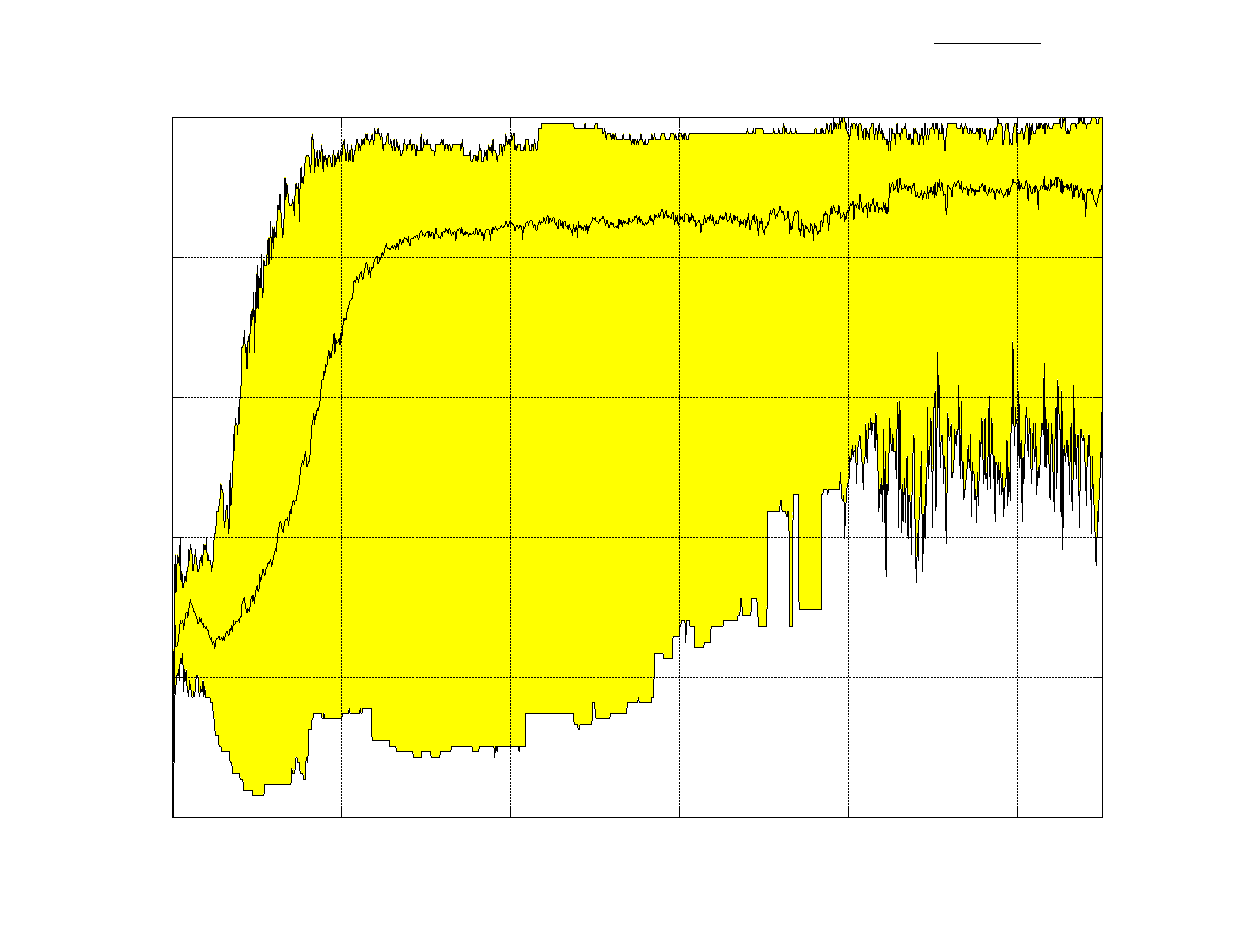
\includegraphics{./images/artificial/gmlaslcs0/adder7_3Mex.eps}}%
    \gplfronttext
  \end{picture}%
\endgroup
}
  	\put(-240,60){\rotatebox{90}{$Exact \: Match$}}
  	\scalebox{0.8}{\put(-180,0){\rotatebox{0}{$iterations$}}}  
  \end{minipage}
\end{figure}

\begin{figure}[ht]
  \caption{Διαγράμματα χαρτογράφησης $adder_{7}^{3}$ του GMl-ASLCS$_{\:0C}$.}
  \label{fig:gmlaslcs0Cadder7_3}
  \begin{minipage}[b]{0.5\linewidth}
  	\centering
  	\scalebox{0.42}{\Large% GNUPLOT: LaTeX picture with Postscript
\begingroup
  \makeatletter
  \providecommand\color[2][]{%
    \GenericError{(gnuplot) \space\space\space\@spaces}{%
      Package color not loaded in conjunction with
      terminal option `colourtext'%
    }{See the gnuplot documentation for explanation.%
    }{Either use 'blacktext' in gnuplot or load the package
      color.sty in LaTeX.}%
    \renewcommand\color[2][]{}%
  }%
  \providecommand\includegraphics[2][]{%
    \GenericError{(gnuplot) \space\space\space\@spaces}{%
      Package graphicx or graphics not loaded%
    }{See the gnuplot documentation for explanation.%
    }{The gnuplot epslatex terminal needs graphicx.sty or graphics.sty.}%
    \renewcommand\includegraphics[2][]{}%
  }%
  \providecommand\rotatebox[2]{#2}%
  \@ifundefined{ifGPcolor}{%
    \newif\ifGPcolor
    \GPcolorfalse
  }{}%
  \@ifundefined{ifGPblacktext}{%
    \newif\ifGPblacktext
    \GPblacktexttrue
  }{}%
  % define a \g@addto@macro without @ in the name:
  \let\gplgaddtomacro\g@addto@macro
  % define empty templates for all commands taking text:
  \gdef\gplbacktext{}%
  \gdef\gplfronttext{}%
  \makeatother
  \ifGPblacktext
    % no textcolor at all
    \def\colorrgb#1{}%
    \def\colorgray#1{}%
  \else
    % gray or color?
    \ifGPcolor
      \def\colorrgb#1{\color[rgb]{#1}}%
      \def\colorgray#1{\color[gray]{#1}}%
      \expandafter\def\csname LTw\endcsname{\color{white}}%
      \expandafter\def\csname LTb\endcsname{\color{black}}%
      \expandafter\def\csname LTa\endcsname{\color{black}}%
      \expandafter\def\csname LT0\endcsname{\color[rgb]{1,0,0}}%
      \expandafter\def\csname LT1\endcsname{\color[rgb]{0,1,0}}%
      \expandafter\def\csname LT2\endcsname{\color[rgb]{0,0,1}}%
      \expandafter\def\csname LT3\endcsname{\color[rgb]{1,0,1}}%
      \expandafter\def\csname LT4\endcsname{\color[rgb]{0,1,1}}%
      \expandafter\def\csname LT5\endcsname{\color[rgb]{1,1,0}}%
      \expandafter\def\csname LT6\endcsname{\color[rgb]{0,0,0}}%
      \expandafter\def\csname LT7\endcsname{\color[rgb]{1,0.3,0}}%
      \expandafter\def\csname LT8\endcsname{\color[rgb]{0.5,0.5,0.5}}%
    \else
      % gray
      \def\colorrgb#1{\color{black}}%
      \def\colorgray#1{\color[gray]{#1}}%
      \expandafter\def\csname LTw\endcsname{\color{white}}%
      \expandafter\def\csname LTb\endcsname{\color{black}}%
      \expandafter\def\csname LTa\endcsname{\color{black}}%
      \expandafter\def\csname LT0\endcsname{\color{black}}%
      \expandafter\def\csname LT1\endcsname{\color{black}}%
      \expandafter\def\csname LT2\endcsname{\color{black}}%
      \expandafter\def\csname LT3\endcsname{\color{black}}%
      \expandafter\def\csname LT4\endcsname{\color{black}}%
      \expandafter\def\csname LT5\endcsname{\color{black}}%
      \expandafter\def\csname LT6\endcsname{\color{black}}%
      \expandafter\def\csname LT7\endcsname{\color{black}}%
      \expandafter\def\csname LT8\endcsname{\color{black}}%
    \fi
  \fi
  \setlength{\unitlength}{0.0500bp}%
  \begin{picture}(11520.00,8640.00)%
    \gplgaddtomacro\gplbacktext{%
    }%
    \gplgaddtomacro\gplfronttext{%
      \csname LTb\endcsname%
      \put(8089,8377){\makebox(0,0)[r]{\strut{}$GMl-ASLCS_{\:0C} \: mean  \:accuracy  \:in  \:adder_7^{3}$}}%
      \colorrgb{0.00,0.00,0.00}%
      \put(1257,950){\makebox(0,0)[r]{\strut{}$0$}}%
      \colorrgb{0.00,0.00,0.00}%
      \put(1257,2294){\makebox(0,0)[r]{\strut{}$0.2$}}%
      \colorrgb{0.00,0.00,0.00}%
      \put(1257,3637){\makebox(0,0)[r]{\strut{}$0.4$}}%
      \colorrgb{0.00,0.00,0.00}%
      \put(1257,4981){\makebox(0,0)[r]{\strut{}$0.6$}}%
      \colorrgb{0.00,0.00,0.00}%
      \put(1257,6324){\makebox(0,0)[r]{\strut{}$0.8$}}%
      \colorrgb{0.00,0.00,0.00}%
      \put(1257,7668){\makebox(0,0)[r]{\strut{}$1$}}%
      \colorrgb{0.00,0.00,0.00}%
      \put(1497,550){\makebox(0,0){\strut{}$0$}}%
      \colorrgb{0.00,0.00,0.00}%
      \put(3120,550){\makebox(0,0){\strut{}$200$}}%
      \colorrgb{0.00,0.00,0.00}%
      \put(4743,550){\makebox(0,0){\strut{}$400$}}%
      \colorrgb{0.00,0.00,0.00}%
      \put(6366,550){\makebox(0,0){\strut{}$600$}}%
      \colorrgb{0.00,0.00,0.00}%
      \put(7989,550){\makebox(0,0){\strut{}$800$}}%
      \colorrgb{0.00,0.00,0.00}%
      \put(9612,550){\makebox(0,0){\strut{}$1000$}}%
    }%
    \gplbacktext
    \put(0,0){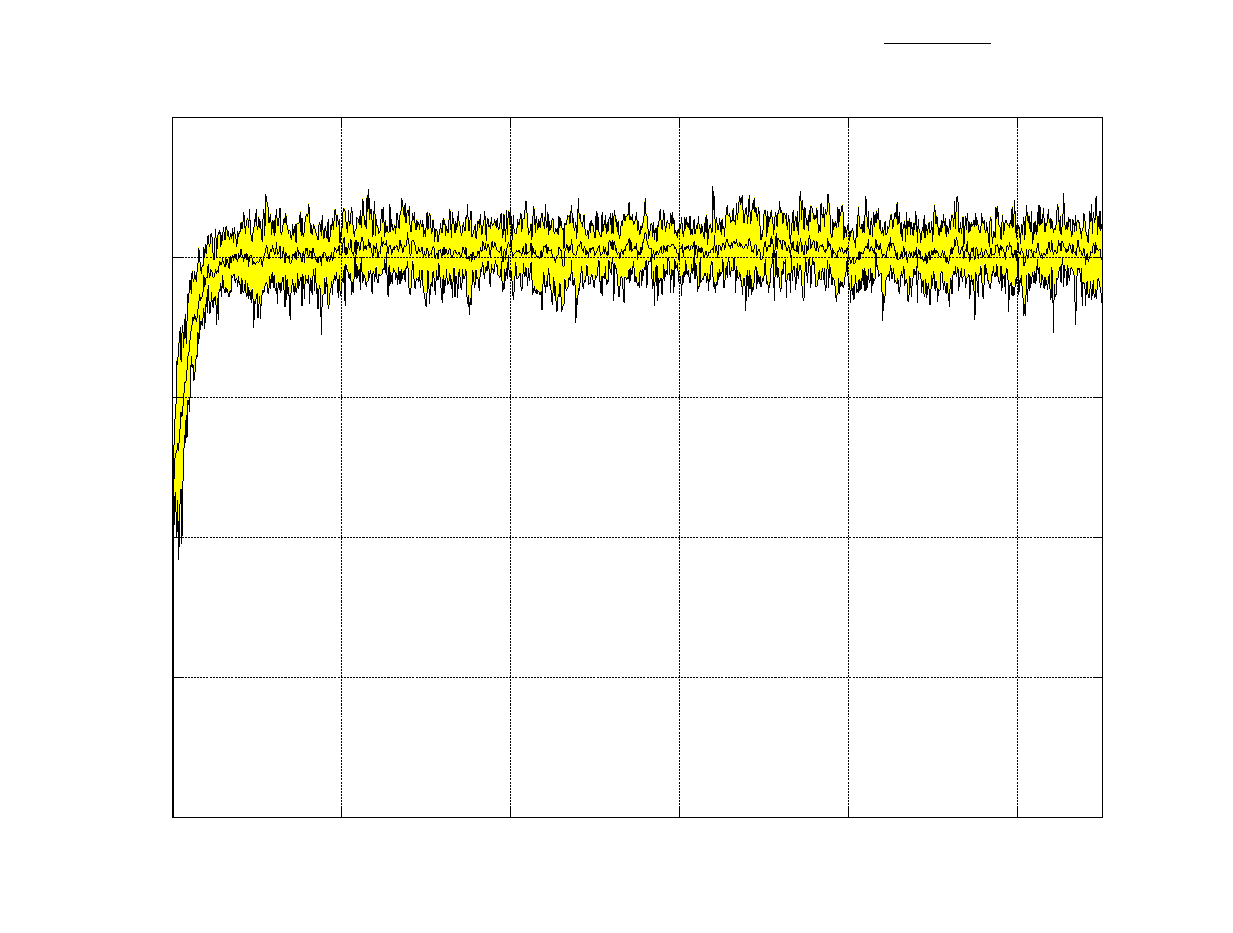
\includegraphics{./images/artificial/gmlaslcs0/adder7_3Cacc.eps}}%
    \gplfronttext
  \end{picture}%
\endgroup
}
  	\put(-240,60){\rotatebox{90}{$Accuracy$}}
 	\scalebox{0.8}{\put(-180,0){\rotatebox{0}{$iterations$}}}  
  	\end{minipage}
  \begin{minipage}[b]{0.5\linewidth}
  	\centering
  	\scalebox{0.42}{\Large% GNUPLOT: LaTeX picture with Postscript
\begingroup
  \makeatletter
  \providecommand\color[2][]{%
    \GenericError{(gnuplot) \space\space\space\@spaces}{%
      Package color not loaded in conjunction with
      terminal option `colourtext'%
    }{See the gnuplot documentation for explanation.%
    }{Either use 'blacktext' in gnuplot or load the package
      color.sty in LaTeX.}%
    \renewcommand\color[2][]{}%
  }%
  \providecommand\includegraphics[2][]{%
    \GenericError{(gnuplot) \space\space\space\@spaces}{%
      Package graphicx or graphics not loaded%
    }{See the gnuplot documentation for explanation.%
    }{The gnuplot epslatex terminal needs graphicx.sty or graphics.sty.}%
    \renewcommand\includegraphics[2][]{}%
  }%
  \providecommand\rotatebox[2]{#2}%
  \@ifundefined{ifGPcolor}{%
    \newif\ifGPcolor
    \GPcolorfalse
  }{}%
  \@ifundefined{ifGPblacktext}{%
    \newif\ifGPblacktext
    \GPblacktexttrue
  }{}%
  % define a \g@addto@macro without @ in the name:
  \let\gplgaddtomacro\g@addto@macro
  % define empty templates for all commands taking text:
  \gdef\gplbacktext{}%
  \gdef\gplfronttext{}%
  \makeatother
  \ifGPblacktext
    % no textcolor at all
    \def\colorrgb#1{}%
    \def\colorgray#1{}%
  \else
    % gray or color?
    \ifGPcolor
      \def\colorrgb#1{\color[rgb]{#1}}%
      \def\colorgray#1{\color[gray]{#1}}%
      \expandafter\def\csname LTw\endcsname{\color{white}}%
      \expandafter\def\csname LTb\endcsname{\color{black}}%
      \expandafter\def\csname LTa\endcsname{\color{black}}%
      \expandafter\def\csname LT0\endcsname{\color[rgb]{1,0,0}}%
      \expandafter\def\csname LT1\endcsname{\color[rgb]{0,1,0}}%
      \expandafter\def\csname LT2\endcsname{\color[rgb]{0,0,1}}%
      \expandafter\def\csname LT3\endcsname{\color[rgb]{1,0,1}}%
      \expandafter\def\csname LT4\endcsname{\color[rgb]{0,1,1}}%
      \expandafter\def\csname LT5\endcsname{\color[rgb]{1,1,0}}%
      \expandafter\def\csname LT6\endcsname{\color[rgb]{0,0,0}}%
      \expandafter\def\csname LT7\endcsname{\color[rgb]{1,0.3,0}}%
      \expandafter\def\csname LT8\endcsname{\color[rgb]{0.5,0.5,0.5}}%
    \else
      % gray
      \def\colorrgb#1{\color{black}}%
      \def\colorgray#1{\color[gray]{#1}}%
      \expandafter\def\csname LTw\endcsname{\color{white}}%
      \expandafter\def\csname LTb\endcsname{\color{black}}%
      \expandafter\def\csname LTa\endcsname{\color{black}}%
      \expandafter\def\csname LT0\endcsname{\color{black}}%
      \expandafter\def\csname LT1\endcsname{\color{black}}%
      \expandafter\def\csname LT2\endcsname{\color{black}}%
      \expandafter\def\csname LT3\endcsname{\color{black}}%
      \expandafter\def\csname LT4\endcsname{\color{black}}%
      \expandafter\def\csname LT5\endcsname{\color{black}}%
      \expandafter\def\csname LT6\endcsname{\color{black}}%
      \expandafter\def\csname LT7\endcsname{\color{black}}%
      \expandafter\def\csname LT8\endcsname{\color{black}}%
    \fi
  \fi
  \setlength{\unitlength}{0.0500bp}%
  \begin{picture}(11520.00,8640.00)%
    \gplgaddtomacro\gplbacktext{%
    }%
    \gplgaddtomacro\gplfronttext{%
      \csname LTb\endcsname%
      \put(8449,8377){\makebox(0,0)[r]{\strut{}$GMl-ASLCS_{\:0C} \: mean  \:exact \: match  \:in  \:adder_7^{3}$}}%
      \colorrgb{0.00,0.00,0.00}%
      \put(1257,950){\makebox(0,0)[r]{\strut{}$0$}}%
      \colorrgb{0.00,0.00,0.00}%
      \put(1257,1790){\makebox(0,0)[r]{\strut{}$0.1$}}%
      \colorrgb{0.00,0.00,0.00}%
      \put(1257,2630){\makebox(0,0)[r]{\strut{}$0.2$}}%
      \colorrgb{0.00,0.00,0.00}%
      \put(1257,3469){\makebox(0,0)[r]{\strut{}$0.3$}}%
      \colorrgb{0.00,0.00,0.00}%
      \put(1257,4309){\makebox(0,0)[r]{\strut{}$0.4$}}%
      \colorrgb{0.00,0.00,0.00}%
      \put(1257,5149){\makebox(0,0)[r]{\strut{}$0.5$}}%
      \colorrgb{0.00,0.00,0.00}%
      \put(1257,5988){\makebox(0,0)[r]{\strut{}$0.6$}}%
      \colorrgb{0.00,0.00,0.00}%
      \put(1257,6828){\makebox(0,0)[r]{\strut{}$0.7$}}%
      \colorrgb{0.00,0.00,0.00}%
      \put(1257,7668){\makebox(0,0)[r]{\strut{}$0.8$}}%
      \colorrgb{0.00,0.00,0.00}%
      \put(1497,550){\makebox(0,0){\strut{}$0$}}%
      \colorrgb{0.00,0.00,0.00}%
      \put(3120,550){\makebox(0,0){\strut{}$200$}}%
      \colorrgb{0.00,0.00,0.00}%
      \put(4743,550){\makebox(0,0){\strut{}$400$}}%
      \colorrgb{0.00,0.00,0.00}%
      \put(6366,550){\makebox(0,0){\strut{}$600$}}%
      \colorrgb{0.00,0.00,0.00}%
      \put(7989,550){\makebox(0,0){\strut{}$800$}}%
      \colorrgb{0.00,0.00,0.00}%
      \put(9612,550){\makebox(0,0){\strut{}$1000$}}%
    }%
    \gplbacktext
    \put(0,0){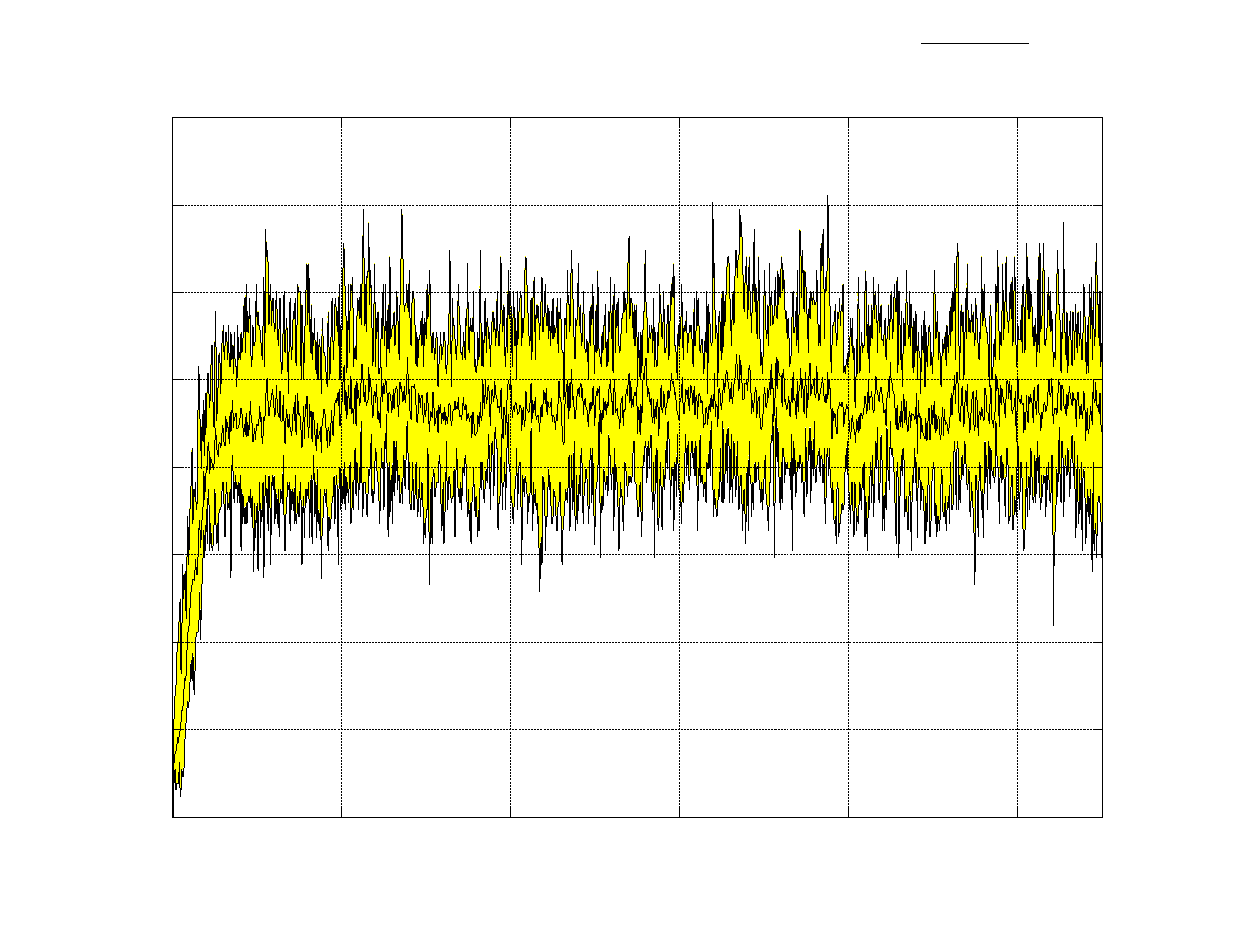
\includegraphics{./images/artificial/gmlaslcs0/adder7_3Cex.eps}}%
    \gplfronttext
  \end{picture}%
\endgroup
}
  	\put(-240,60){\rotatebox{90}{$Exact \: Match$}}
  	\scalebox{0.8}{\put(-180,0){\rotatebox{0}{$iterations$}}}  
  \end{minipage}
\end{figure}







%\clearpage
%-----------------------------------------adder7_24-----------------------------------------%

\subsection{Οι τροποποιημένοι αλγόριθμοι GMl-ASLCS$_{\:0*}$ στο πρόβλημα $adder_{7}^{24}$}
Τα Σχήματα \ref{fig:gmlaslcs0Dadder7_24}, \ref{fig:gmlaslcs0GAadder7_24}, \ref{fig:gmlaslcs0Madder7_24} και \ref{fig:gmlaslcs0Cadder7_24} παρουσιάζουν την εξέλιξη των μετρικών της Ακρίβειας και της Ακριβούς Ορθότητας για το σύνολο δεδομένων  $adder_{7}^{24}$, των ΜαΣΤ GMl-ASLCS$_{\:0D}$, GMl-ASLCS$_{\:0GA}$, GMl-ASLCS$_{\:0M}$ και GMl-ASLCS$_{\:0C}$, αντίστοιχα.

\begin{figure}[ht]
  \caption{Διαγράμματα χαρτογράφησης $adder_{7}^{24}$ του GMl-ASLCS$_{\:0D}$.}
  \label{fig:gmlaslcs0Dadder7_24}
  \begin{minipage}[b]{0.5\linewidth}
  	\centering
  	\scalebox{0.42}{\Large% GNUPLOT: LaTeX picture with Postscript
\begingroup
  \makeatletter
  \providecommand\color[2][]{%
    \GenericError{(gnuplot) \space\space\space\@spaces}{%
      Package color not loaded in conjunction with
      terminal option `colourtext'%
    }{See the gnuplot documentation for explanation.%
    }{Either use 'blacktext' in gnuplot or load the package
      color.sty in LaTeX.}%
    \renewcommand\color[2][]{}%
  }%
  \providecommand\includegraphics[2][]{%
    \GenericError{(gnuplot) \space\space\space\@spaces}{%
      Package graphicx or graphics not loaded%
    }{See the gnuplot documentation for explanation.%
    }{The gnuplot epslatex terminal needs graphicx.sty or graphics.sty.}%
    \renewcommand\includegraphics[2][]{}%
  }%
  \providecommand\rotatebox[2]{#2}%
  \@ifundefined{ifGPcolor}{%
    \newif\ifGPcolor
    \GPcolorfalse
  }{}%
  \@ifundefined{ifGPblacktext}{%
    \newif\ifGPblacktext
    \GPblacktexttrue
  }{}%
  % define a \g@addto@macro without @ in the name:
  \let\gplgaddtomacro\g@addto@macro
  % define empty templates for all commands taking text:
  \gdef\gplbacktext{}%
  \gdef\gplfronttext{}%
  \makeatother
  \ifGPblacktext
    % no textcolor at all
    \def\colorrgb#1{}%
    \def\colorgray#1{}%
  \else
    % gray or color?
    \ifGPcolor
      \def\colorrgb#1{\color[rgb]{#1}}%
      \def\colorgray#1{\color[gray]{#1}}%
      \expandafter\def\csname LTw\endcsname{\color{white}}%
      \expandafter\def\csname LTb\endcsname{\color{black}}%
      \expandafter\def\csname LTa\endcsname{\color{black}}%
      \expandafter\def\csname LT0\endcsname{\color[rgb]{1,0,0}}%
      \expandafter\def\csname LT1\endcsname{\color[rgb]{0,1,0}}%
      \expandafter\def\csname LT2\endcsname{\color[rgb]{0,0,1}}%
      \expandafter\def\csname LT3\endcsname{\color[rgb]{1,0,1}}%
      \expandafter\def\csname LT4\endcsname{\color[rgb]{0,1,1}}%
      \expandafter\def\csname LT5\endcsname{\color[rgb]{1,1,0}}%
      \expandafter\def\csname LT6\endcsname{\color[rgb]{0,0,0}}%
      \expandafter\def\csname LT7\endcsname{\color[rgb]{1,0.3,0}}%
      \expandafter\def\csname LT8\endcsname{\color[rgb]{0.5,0.5,0.5}}%
    \else
      % gray
      \def\colorrgb#1{\color{black}}%
      \def\colorgray#1{\color[gray]{#1}}%
      \expandafter\def\csname LTw\endcsname{\color{white}}%
      \expandafter\def\csname LTb\endcsname{\color{black}}%
      \expandafter\def\csname LTa\endcsname{\color{black}}%
      \expandafter\def\csname LT0\endcsname{\color{black}}%
      \expandafter\def\csname LT1\endcsname{\color{black}}%
      \expandafter\def\csname LT2\endcsname{\color{black}}%
      \expandafter\def\csname LT3\endcsname{\color{black}}%
      \expandafter\def\csname LT4\endcsname{\color{black}}%
      \expandafter\def\csname LT5\endcsname{\color{black}}%
      \expandafter\def\csname LT6\endcsname{\color{black}}%
      \expandafter\def\csname LT7\endcsname{\color{black}}%
      \expandafter\def\csname LT8\endcsname{\color{black}}%
    \fi
  \fi
  \setlength{\unitlength}{0.0500bp}%
  \begin{picture}(11520.00,8640.00)%
    \gplgaddtomacro\gplbacktext{%
    }%
    \gplgaddtomacro\gplfronttext{%
      \csname LTb\endcsname%
      \put(8329,8377){\makebox(0,0)[r]{\strut{}$GMl-ASLCS_{\:0D} \: mean \: accuracy  \:in \: adder_7^{24}$}}%
      \colorrgb{0.00,0.00,0.00}%
      \put(1257,950){\makebox(0,0)[r]{\strut{}$0$}}%
      \colorrgb{0.00,0.00,0.00}%
      \put(1257,2294){\makebox(0,0)[r]{\strut{}$0.2$}}%
      \colorrgb{0.00,0.00,0.00}%
      \put(1257,3637){\makebox(0,0)[r]{\strut{}$0.4$}}%
      \colorrgb{0.00,0.00,0.00}%
      \put(1257,4981){\makebox(0,0)[r]{\strut{}$0.6$}}%
      \colorrgb{0.00,0.00,0.00}%
      \put(1257,6324){\makebox(0,0)[r]{\strut{}$0.8$}}%
      \colorrgb{0.00,0.00,0.00}%
      \put(1257,7668){\makebox(0,0)[r]{\strut{}$1$}}%
      \colorrgb{0.00,0.00,0.00}%
      \put(1497,550){\makebox(0,0){\strut{}$0$}}%
      \colorrgb{0.00,0.00,0.00}%
      \put(3120,550){\makebox(0,0){\strut{}$200$}}%
      \colorrgb{0.00,0.00,0.00}%
      \put(4743,550){\makebox(0,0){\strut{}$400$}}%
      \colorrgb{0.00,0.00,0.00}%
      \put(6366,550){\makebox(0,0){\strut{}$600$}}%
      \colorrgb{0.00,0.00,0.00}%
      \put(7989,550){\makebox(0,0){\strut{}$800$}}%
      \colorrgb{0.00,0.00,0.00}%
      \put(9612,550){\makebox(0,0){\strut{}$1000$}}%
    }%
    \gplbacktext
    \put(0,0){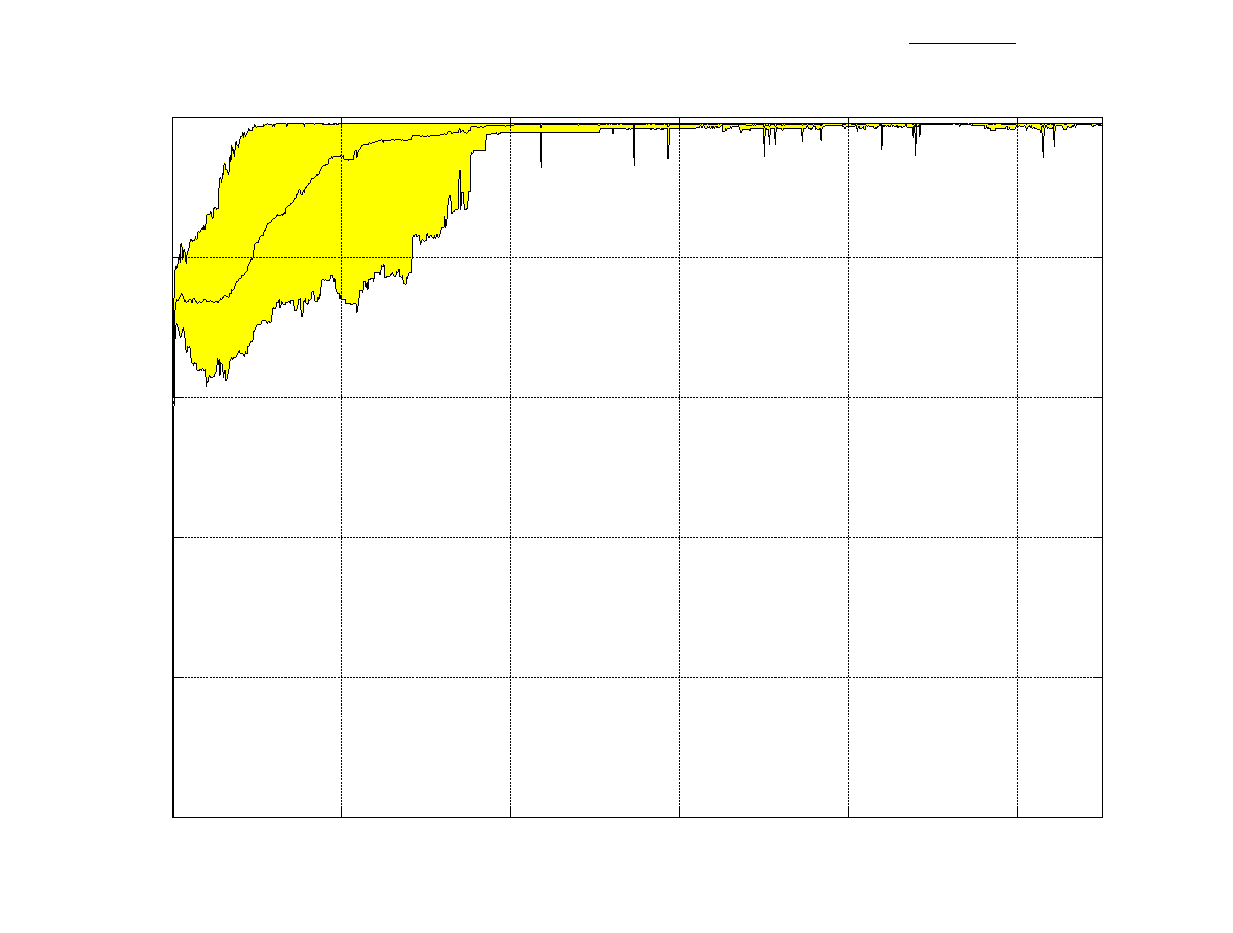
\includegraphics{./images/artificial/gmlaslcs0/adder7_24Dacc.eps}}%
    \gplfronttext
  \end{picture}%
\endgroup
}
  	\put(-240,60){\rotatebox{90}{$Accuracy$}}
 	\scalebox{0.8}{\put(-180,0){\rotatebox{0}{$iterations$}}}  
  	\end{minipage}
  \begin{minipage}[b]{0.5\linewidth}
  	\centering
  	\scalebox{0.42}{\Large% GNUPLOT: LaTeX picture with Postscript
\begingroup
  \makeatletter
  \providecommand\color[2][]{%
    \GenericError{(gnuplot) \space\space\space\@spaces}{%
      Package color not loaded in conjunction with
      terminal option `colourtext'%
    }{See the gnuplot documentation for explanation.%
    }{Either use 'blacktext' in gnuplot or load the package
      color.sty in LaTeX.}%
    \renewcommand\color[2][]{}%
  }%
  \providecommand\includegraphics[2][]{%
    \GenericError{(gnuplot) \space\space\space\@spaces}{%
      Package graphicx or graphics not loaded%
    }{See the gnuplot documentation for explanation.%
    }{The gnuplot epslatex terminal needs graphicx.sty or graphics.sty.}%
    \renewcommand\includegraphics[2][]{}%
  }%
  \providecommand\rotatebox[2]{#2}%
  \@ifundefined{ifGPcolor}{%
    \newif\ifGPcolor
    \GPcolorfalse
  }{}%
  \@ifundefined{ifGPblacktext}{%
    \newif\ifGPblacktext
    \GPblacktexttrue
  }{}%
  % define a \g@addto@macro without @ in the name:
  \let\gplgaddtomacro\g@addto@macro
  % define empty templates for all commands taking text:
  \gdef\gplbacktext{}%
  \gdef\gplfronttext{}%
  \makeatother
  \ifGPblacktext
    % no textcolor at all
    \def\colorrgb#1{}%
    \def\colorgray#1{}%
  \else
    % gray or color?
    \ifGPcolor
      \def\colorrgb#1{\color[rgb]{#1}}%
      \def\colorgray#1{\color[gray]{#1}}%
      \expandafter\def\csname LTw\endcsname{\color{white}}%
      \expandafter\def\csname LTb\endcsname{\color{black}}%
      \expandafter\def\csname LTa\endcsname{\color{black}}%
      \expandafter\def\csname LT0\endcsname{\color[rgb]{1,0,0}}%
      \expandafter\def\csname LT1\endcsname{\color[rgb]{0,1,0}}%
      \expandafter\def\csname LT2\endcsname{\color[rgb]{0,0,1}}%
      \expandafter\def\csname LT3\endcsname{\color[rgb]{1,0,1}}%
      \expandafter\def\csname LT4\endcsname{\color[rgb]{0,1,1}}%
      \expandafter\def\csname LT5\endcsname{\color[rgb]{1,1,0}}%
      \expandafter\def\csname LT6\endcsname{\color[rgb]{0,0,0}}%
      \expandafter\def\csname LT7\endcsname{\color[rgb]{1,0.3,0}}%
      \expandafter\def\csname LT8\endcsname{\color[rgb]{0.5,0.5,0.5}}%
    \else
      % gray
      \def\colorrgb#1{\color{black}}%
      \def\colorgray#1{\color[gray]{#1}}%
      \expandafter\def\csname LTw\endcsname{\color{white}}%
      \expandafter\def\csname LTb\endcsname{\color{black}}%
      \expandafter\def\csname LTa\endcsname{\color{black}}%
      \expandafter\def\csname LT0\endcsname{\color{black}}%
      \expandafter\def\csname LT1\endcsname{\color{black}}%
      \expandafter\def\csname LT2\endcsname{\color{black}}%
      \expandafter\def\csname LT3\endcsname{\color{black}}%
      \expandafter\def\csname LT4\endcsname{\color{black}}%
      \expandafter\def\csname LT5\endcsname{\color{black}}%
      \expandafter\def\csname LT6\endcsname{\color{black}}%
      \expandafter\def\csname LT7\endcsname{\color{black}}%
      \expandafter\def\csname LT8\endcsname{\color{black}}%
    \fi
  \fi
  \setlength{\unitlength}{0.0500bp}%
  \begin{picture}(11520.00,8640.00)%
    \gplgaddtomacro\gplbacktext{%
    }%
    \gplgaddtomacro\gplfronttext{%
      \csname LTb\endcsname%
      \put(8689,8377){\makebox(0,0)[r]{\strut{}$GMl-ASLCS_{\:0D} \: mean  \:exact \: match  \:in \: adder_7^{24}$}}%
      \colorrgb{0.00,0.00,0.00}%
      \put(1257,950){\makebox(0,0)[r]{\strut{}$0$}}%
      \colorrgb{0.00,0.00,0.00}%
      \put(1257,2294){\makebox(0,0)[r]{\strut{}$0.2$}}%
      \colorrgb{0.00,0.00,0.00}%
      \put(1257,3637){\makebox(0,0)[r]{\strut{}$0.4$}}%
      \colorrgb{0.00,0.00,0.00}%
      \put(1257,4981){\makebox(0,0)[r]{\strut{}$0.6$}}%
      \colorrgb{0.00,0.00,0.00}%
      \put(1257,6324){\makebox(0,0)[r]{\strut{}$0.8$}}%
      \colorrgb{0.00,0.00,0.00}%
      \put(1257,7668){\makebox(0,0)[r]{\strut{}$1$}}%
      \colorrgb{0.00,0.00,0.00}%
      \put(1497,550){\makebox(0,0){\strut{}$0$}}%
      \colorrgb{0.00,0.00,0.00}%
      \put(3120,550){\makebox(0,0){\strut{}$200$}}%
      \colorrgb{0.00,0.00,0.00}%
      \put(4743,550){\makebox(0,0){\strut{}$400$}}%
      \colorrgb{0.00,0.00,0.00}%
      \put(6366,550){\makebox(0,0){\strut{}$600$}}%
      \colorrgb{0.00,0.00,0.00}%
      \put(7989,550){\makebox(0,0){\strut{}$800$}}%
      \colorrgb{0.00,0.00,0.00}%
      \put(9612,550){\makebox(0,0){\strut{}$1000$}}%
    }%
    \gplbacktext
    \put(0,0){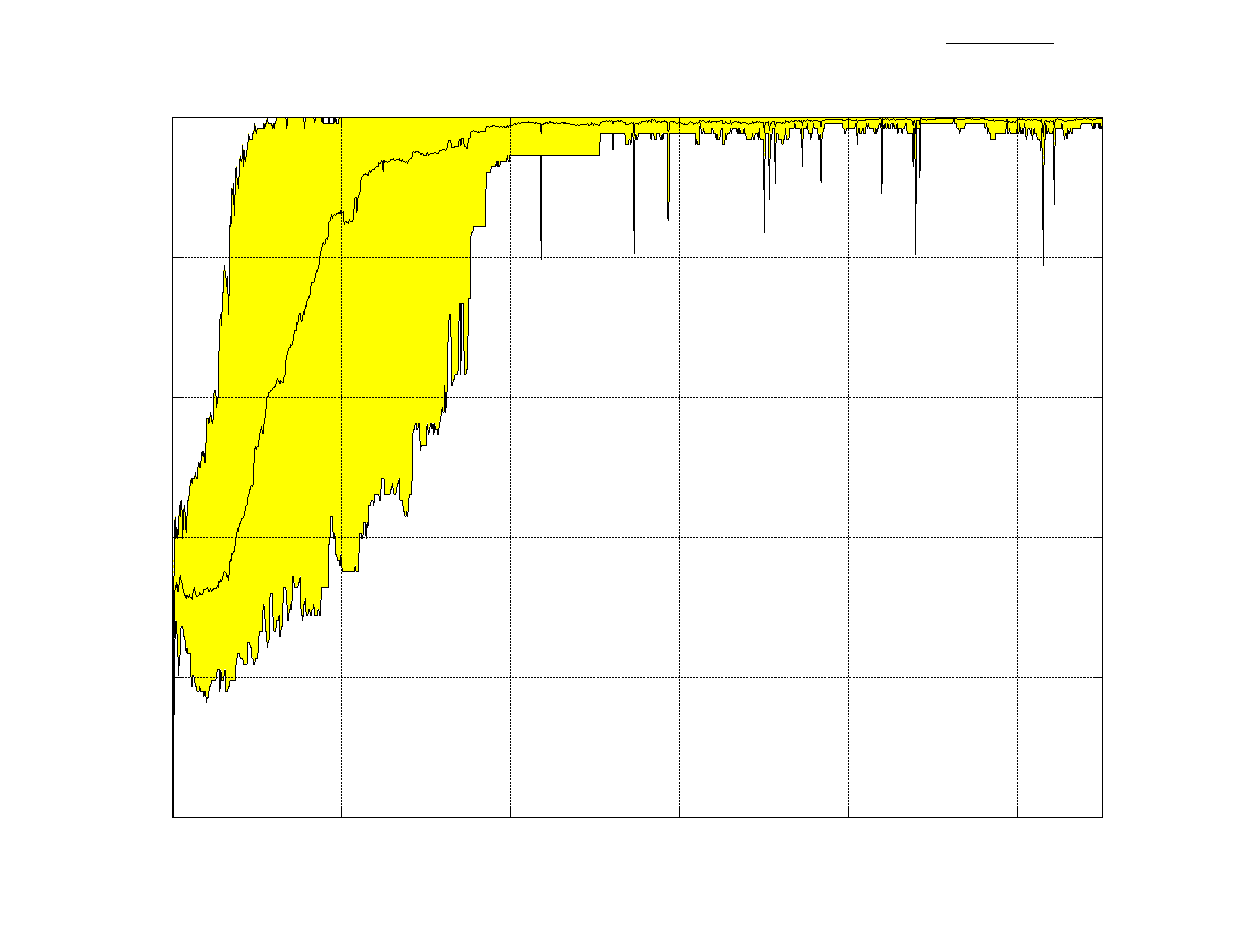
\includegraphics{./images/artificial/gmlaslcs0/adder7_24Dex.eps}}%
    \gplfronttext
  \end{picture}%
\endgroup
}
  	\put(-240,60){\rotatebox{90}{$Exact \: Match$}}
  	\scalebox{0.8}{\put(-180,0){\rotatebox{0}{$iterations$}}}  
  \end{minipage}
\end{figure}

\begin{figure}[ht]
  \caption{Διαγράμματα χαρτογράφησης $adder_{7}^{24}$ του GMl-ASLCS$_{\:0GA}$.}
  \label{fig:gmlaslcs0GAadder7_24}
  \begin{minipage}[b]{0.5\linewidth}
  	\centering
  	\scalebox{0.42}{\Large% GNUPLOT: LaTeX picture with Postscript
\begingroup
  \makeatletter
  \providecommand\color[2][]{%
    \GenericError{(gnuplot) \space\space\space\@spaces}{%
      Package color not loaded in conjunction with
      terminal option `colourtext'%
    }{See the gnuplot documentation for explanation.%
    }{Either use 'blacktext' in gnuplot or load the package
      color.sty in LaTeX.}%
    \renewcommand\color[2][]{}%
  }%
  \providecommand\includegraphics[2][]{%
    \GenericError{(gnuplot) \space\space\space\@spaces}{%
      Package graphicx or graphics not loaded%
    }{See the gnuplot documentation for explanation.%
    }{The gnuplot epslatex terminal needs graphicx.sty or graphics.sty.}%
    \renewcommand\includegraphics[2][]{}%
  }%
  \providecommand\rotatebox[2]{#2}%
  \@ifundefined{ifGPcolor}{%
    \newif\ifGPcolor
    \GPcolorfalse
  }{}%
  \@ifundefined{ifGPblacktext}{%
    \newif\ifGPblacktext
    \GPblacktexttrue
  }{}%
  % define a \g@addto@macro without @ in the name:
  \let\gplgaddtomacro\g@addto@macro
  % define empty templates for all commands taking text:
  \gdef\gplbacktext{}%
  \gdef\gplfronttext{}%
  \makeatother
  \ifGPblacktext
    % no textcolor at all
    \def\colorrgb#1{}%
    \def\colorgray#1{}%
  \else
    % gray or color?
    \ifGPcolor
      \def\colorrgb#1{\color[rgb]{#1}}%
      \def\colorgray#1{\color[gray]{#1}}%
      \expandafter\def\csname LTw\endcsname{\color{white}}%
      \expandafter\def\csname LTb\endcsname{\color{black}}%
      \expandafter\def\csname LTa\endcsname{\color{black}}%
      \expandafter\def\csname LT0\endcsname{\color[rgb]{1,0,0}}%
      \expandafter\def\csname LT1\endcsname{\color[rgb]{0,1,0}}%
      \expandafter\def\csname LT2\endcsname{\color[rgb]{0,0,1}}%
      \expandafter\def\csname LT3\endcsname{\color[rgb]{1,0,1}}%
      \expandafter\def\csname LT4\endcsname{\color[rgb]{0,1,1}}%
      \expandafter\def\csname LT5\endcsname{\color[rgb]{1,1,0}}%
      \expandafter\def\csname LT6\endcsname{\color[rgb]{0,0,0}}%
      \expandafter\def\csname LT7\endcsname{\color[rgb]{1,0.3,0}}%
      \expandafter\def\csname LT8\endcsname{\color[rgb]{0.5,0.5,0.5}}%
    \else
      % gray
      \def\colorrgb#1{\color{black}}%
      \def\colorgray#1{\color[gray]{#1}}%
      \expandafter\def\csname LTw\endcsname{\color{white}}%
      \expandafter\def\csname LTb\endcsname{\color{black}}%
      \expandafter\def\csname LTa\endcsname{\color{black}}%
      \expandafter\def\csname LT0\endcsname{\color{black}}%
      \expandafter\def\csname LT1\endcsname{\color{black}}%
      \expandafter\def\csname LT2\endcsname{\color{black}}%
      \expandafter\def\csname LT3\endcsname{\color{black}}%
      \expandafter\def\csname LT4\endcsname{\color{black}}%
      \expandafter\def\csname LT5\endcsname{\color{black}}%
      \expandafter\def\csname LT6\endcsname{\color{black}}%
      \expandafter\def\csname LT7\endcsname{\color{black}}%
      \expandafter\def\csname LT8\endcsname{\color{black}}%
    \fi
  \fi
  \setlength{\unitlength}{0.0500bp}%
  \begin{picture}(11520.00,8640.00)%
    \gplgaddtomacro\gplbacktext{%
    }%
    \gplgaddtomacro\gplfronttext{%
      \csname LTb\endcsname%
      \put(8329,8377){\makebox(0,0)[r]{\strut{}$GMl-ASLCS_{\:0GA} \: mean \: accuracy  \:in \:adder_7^{24}$}}%
      \colorrgb{0.00,0.00,0.00}%
      \put(1257,950){\makebox(0,0)[r]{\strut{}$0$}}%
      \colorrgb{0.00,0.00,0.00}%
      \put(1257,2294){\makebox(0,0)[r]{\strut{}$0.2$}}%
      \colorrgb{0.00,0.00,0.00}%
      \put(1257,3637){\makebox(0,0)[r]{\strut{}$0.4$}}%
      \colorrgb{0.00,0.00,0.00}%
      \put(1257,4981){\makebox(0,0)[r]{\strut{}$0.6$}}%
      \colorrgb{0.00,0.00,0.00}%
      \put(1257,6324){\makebox(0,0)[r]{\strut{}$0.8$}}%
      \colorrgb{0.00,0.00,0.00}%
      \put(1257,7668){\makebox(0,0)[r]{\strut{}$1$}}%
      \colorrgb{0.00,0.00,0.00}%
      \put(1497,550){\makebox(0,0){\strut{}$0$}}%
      \colorrgb{0.00,0.00,0.00}%
      \put(3120,550){\makebox(0,0){\strut{}$200$}}%
      \colorrgb{0.00,0.00,0.00}%
      \put(4743,550){\makebox(0,0){\strut{}$400$}}%
      \colorrgb{0.00,0.00,0.00}%
      \put(6366,550){\makebox(0,0){\strut{}$600$}}%
      \colorrgb{0.00,0.00,0.00}%
      \put(7989,550){\makebox(0,0){\strut{}$800$}}%
      \colorrgb{0.00,0.00,0.00}%
      \put(9612,550){\makebox(0,0){\strut{}$1000$}}%
    }%
    \gplbacktext
    \put(0,0){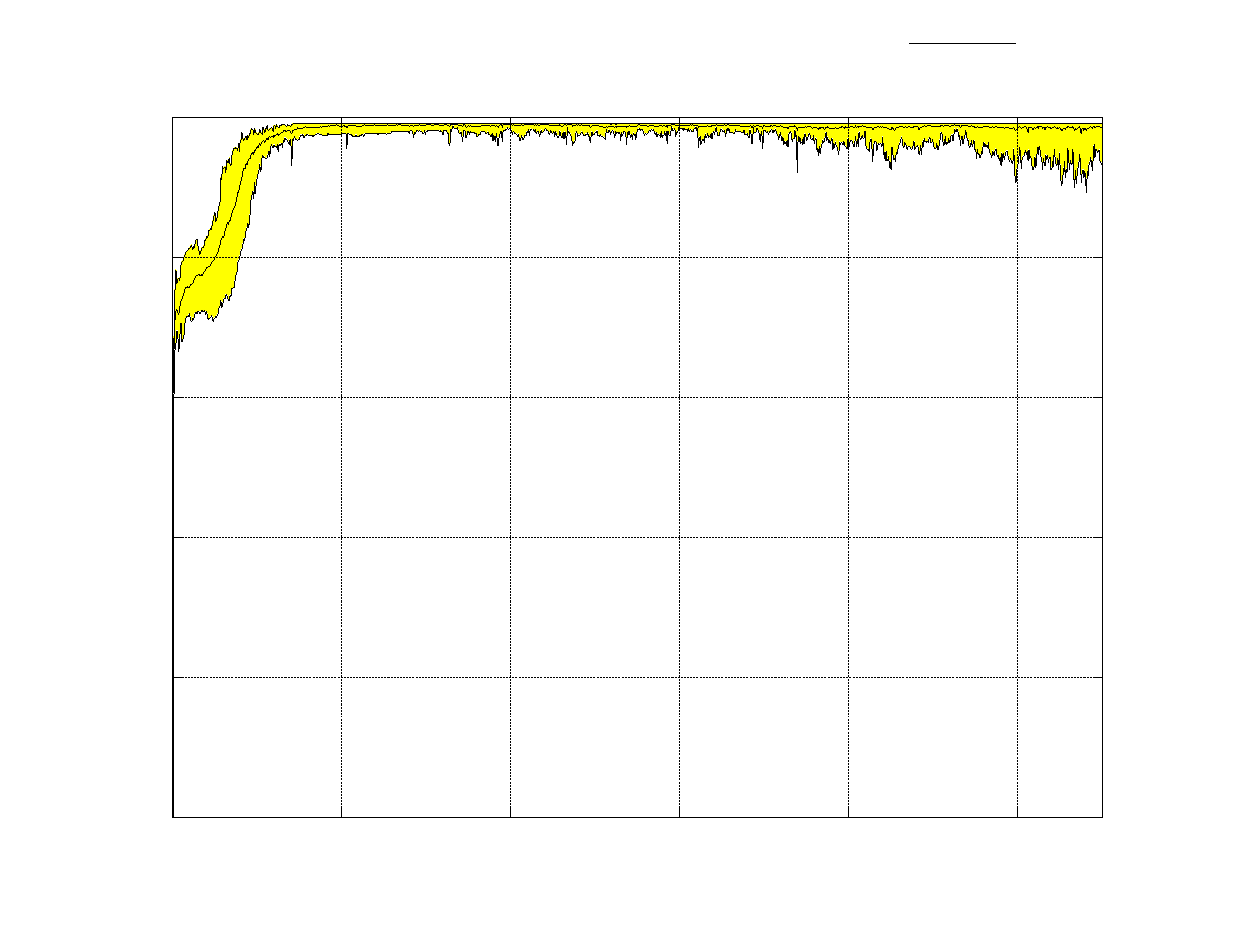
\includegraphics{./images/artificial/gmlaslcs0/adder7_24GAacc.eps}}%
    \gplfronttext
  \end{picture}%
\endgroup
}
  	\put(-240,60){\rotatebox{90}{$Accuracy$}}
 	\scalebox{0.8}{\put(-180,0){\rotatebox{0}{$iterations$}}}  
  	\end{minipage}
  \begin{minipage}[b]{0.5\linewidth}
  	\centering
  	\scalebox{0.42}{\Large% GNUPLOT: LaTeX picture with Postscript
\begingroup
  \makeatletter
  \providecommand\color[2][]{%
    \GenericError{(gnuplot) \space\space\space\@spaces}{%
      Package color not loaded in conjunction with
      terminal option `colourtext'%
    }{See the gnuplot documentation for explanation.%
    }{Either use 'blacktext' in gnuplot or load the package
      color.sty in LaTeX.}%
    \renewcommand\color[2][]{}%
  }%
  \providecommand\includegraphics[2][]{%
    \GenericError{(gnuplot) \space\space\space\@spaces}{%
      Package graphicx or graphics not loaded%
    }{See the gnuplot documentation for explanation.%
    }{The gnuplot epslatex terminal needs graphicx.sty or graphics.sty.}%
    \renewcommand\includegraphics[2][]{}%
  }%
  \providecommand\rotatebox[2]{#2}%
  \@ifundefined{ifGPcolor}{%
    \newif\ifGPcolor
    \GPcolorfalse
  }{}%
  \@ifundefined{ifGPblacktext}{%
    \newif\ifGPblacktext
    \GPblacktexttrue
  }{}%
  % define a \g@addto@macro without @ in the name:
  \let\gplgaddtomacro\g@addto@macro
  % define empty templates for all commands taking text:
  \gdef\gplbacktext{}%
  \gdef\gplfronttext{}%
  \makeatother
  \ifGPblacktext
    % no textcolor at all
    \def\colorrgb#1{}%
    \def\colorgray#1{}%
  \else
    % gray or color?
    \ifGPcolor
      \def\colorrgb#1{\color[rgb]{#1}}%
      \def\colorgray#1{\color[gray]{#1}}%
      \expandafter\def\csname LTw\endcsname{\color{white}}%
      \expandafter\def\csname LTb\endcsname{\color{black}}%
      \expandafter\def\csname LTa\endcsname{\color{black}}%
      \expandafter\def\csname LT0\endcsname{\color[rgb]{1,0,0}}%
      \expandafter\def\csname LT1\endcsname{\color[rgb]{0,1,0}}%
      \expandafter\def\csname LT2\endcsname{\color[rgb]{0,0,1}}%
      \expandafter\def\csname LT3\endcsname{\color[rgb]{1,0,1}}%
      \expandafter\def\csname LT4\endcsname{\color[rgb]{0,1,1}}%
      \expandafter\def\csname LT5\endcsname{\color[rgb]{1,1,0}}%
      \expandafter\def\csname LT6\endcsname{\color[rgb]{0,0,0}}%
      \expandafter\def\csname LT7\endcsname{\color[rgb]{1,0.3,0}}%
      \expandafter\def\csname LT8\endcsname{\color[rgb]{0.5,0.5,0.5}}%
    \else
      % gray
      \def\colorrgb#1{\color{black}}%
      \def\colorgray#1{\color[gray]{#1}}%
      \expandafter\def\csname LTw\endcsname{\color{white}}%
      \expandafter\def\csname LTb\endcsname{\color{black}}%
      \expandafter\def\csname LTa\endcsname{\color{black}}%
      \expandafter\def\csname LT0\endcsname{\color{black}}%
      \expandafter\def\csname LT1\endcsname{\color{black}}%
      \expandafter\def\csname LT2\endcsname{\color{black}}%
      \expandafter\def\csname LT3\endcsname{\color{black}}%
      \expandafter\def\csname LT4\endcsname{\color{black}}%
      \expandafter\def\csname LT5\endcsname{\color{black}}%
      \expandafter\def\csname LT6\endcsname{\color{black}}%
      \expandafter\def\csname LT7\endcsname{\color{black}}%
      \expandafter\def\csname LT8\endcsname{\color{black}}%
    \fi
  \fi
  \setlength{\unitlength}{0.0500bp}%
  \begin{picture}(11520.00,8640.00)%
    \gplgaddtomacro\gplbacktext{%
    }%
    \gplgaddtomacro\gplfronttext{%
      \csname LTb\endcsname%
      \put(8689,8377){\makebox(0,0)[r]{\strut{}$GMl-ASLCS_{\:0GA} \: mean \: exact  \:match \: in  \:adder_7^{24}$}}%
      \colorrgb{0.00,0.00,0.00}%
      \put(1257,950){\makebox(0,0)[r]{\strut{}$0$}}%
      \colorrgb{0.00,0.00,0.00}%
      \put(1257,2294){\makebox(0,0)[r]{\strut{}$0.2$}}%
      \colorrgb{0.00,0.00,0.00}%
      \put(1257,3637){\makebox(0,0)[r]{\strut{}$0.4$}}%
      \colorrgb{0.00,0.00,0.00}%
      \put(1257,4981){\makebox(0,0)[r]{\strut{}$0.6$}}%
      \colorrgb{0.00,0.00,0.00}%
      \put(1257,6324){\makebox(0,0)[r]{\strut{}$0.8$}}%
      \colorrgb{0.00,0.00,0.00}%
      \put(1257,7668){\makebox(0,0)[r]{\strut{}$1$}}%
      \colorrgb{0.00,0.00,0.00}%
      \put(1497,550){\makebox(0,0){\strut{}$0$}}%
      \colorrgb{0.00,0.00,0.00}%
      \put(3120,550){\makebox(0,0){\strut{}$200$}}%
      \colorrgb{0.00,0.00,0.00}%
      \put(4743,550){\makebox(0,0){\strut{}$400$}}%
      \colorrgb{0.00,0.00,0.00}%
      \put(6366,550){\makebox(0,0){\strut{}$600$}}%
      \colorrgb{0.00,0.00,0.00}%
      \put(7989,550){\makebox(0,0){\strut{}$800$}}%
      \colorrgb{0.00,0.00,0.00}%
      \put(9612,550){\makebox(0,0){\strut{}$1000$}}%
    }%
    \gplbacktext
    \put(0,0){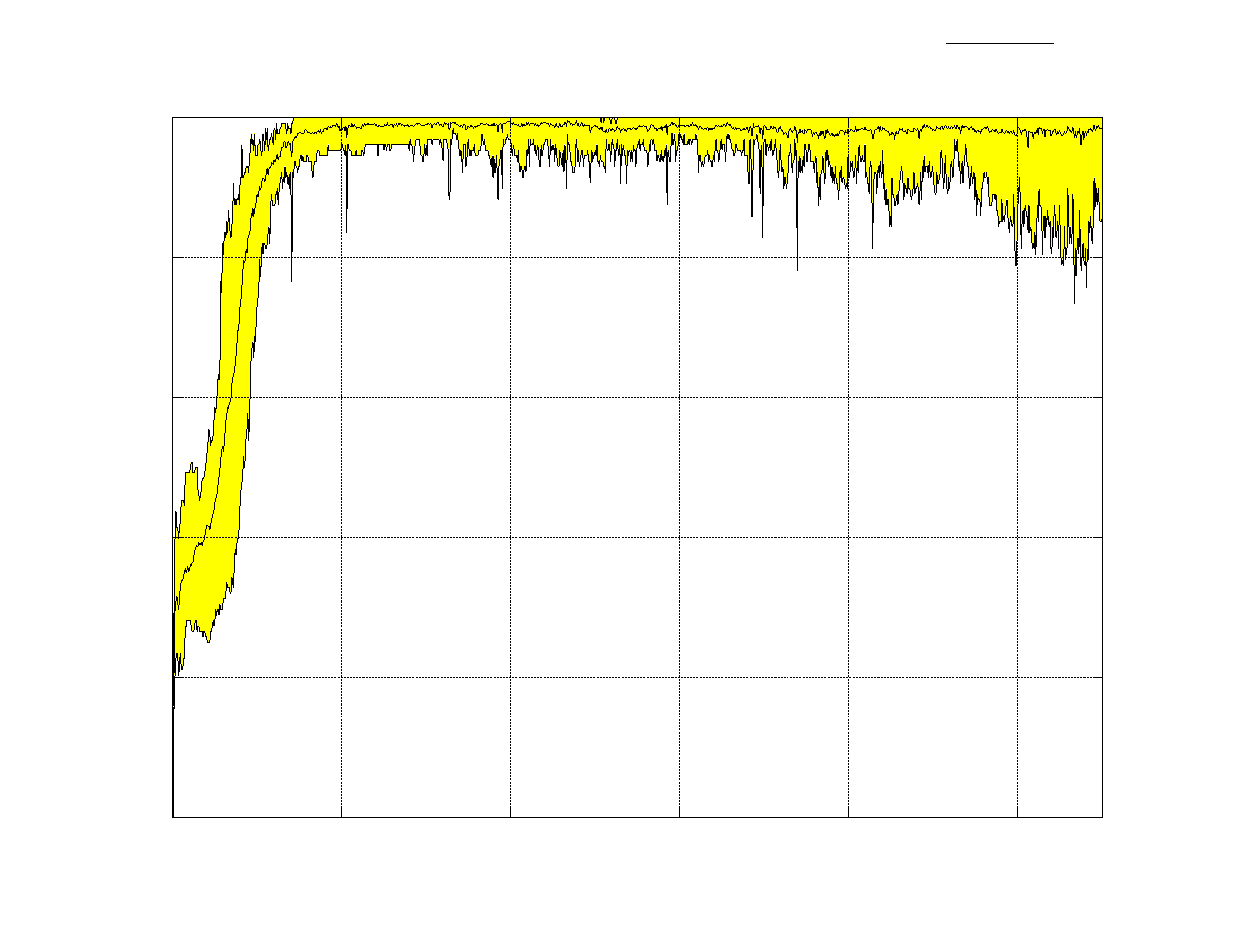
\includegraphics{./images/artificial/gmlaslcs0/adder7_24GAex.eps}}%
    \gplfronttext
  \end{picture}%
\endgroup
}
  	\put(-240,60){\rotatebox{90}{$Exact \: Match$}}
  	\scalebox{0.8}{\put(-180,0){\rotatebox{0}{$iterations$}}}  
  \end{minipage}
\end{figure}

\begin{figure}[ht]
  \caption{Διαγράμματα χαρτογράφησης $adder_{7}^{24}$ του GMl-ASLCS$_{\:0M}$.}
  \label{fig:gmlaslcs0Madder7_24}
  \begin{minipage}[b]{0.5\linewidth}
  	\centering
  	\scalebox{0.42}{\Large% GNUPLOT: LaTeX picture with Postscript
\begingroup
  \makeatletter
  \providecommand\color[2][]{%
    \GenericError{(gnuplot) \space\space\space\@spaces}{%
      Package color not loaded in conjunction with
      terminal option `colourtext'%
    }{See the gnuplot documentation for explanation.%
    }{Either use 'blacktext' in gnuplot or load the package
      color.sty in LaTeX.}%
    \renewcommand\color[2][]{}%
  }%
  \providecommand\includegraphics[2][]{%
    \GenericError{(gnuplot) \space\space\space\@spaces}{%
      Package graphicx or graphics not loaded%
    }{See the gnuplot documentation for explanation.%
    }{The gnuplot epslatex terminal needs graphicx.sty or graphics.sty.}%
    \renewcommand\includegraphics[2][]{}%
  }%
  \providecommand\rotatebox[2]{#2}%
  \@ifundefined{ifGPcolor}{%
    \newif\ifGPcolor
    \GPcolorfalse
  }{}%
  \@ifundefined{ifGPblacktext}{%
    \newif\ifGPblacktext
    \GPblacktexttrue
  }{}%
  % define a \g@addto@macro without @ in the name:
  \let\gplgaddtomacro\g@addto@macro
  % define empty templates for all commands taking text:
  \gdef\gplbacktext{}%
  \gdef\gplfronttext{}%
  \makeatother
  \ifGPblacktext
    % no textcolor at all
    \def\colorrgb#1{}%
    \def\colorgray#1{}%
  \else
    % gray or color?
    \ifGPcolor
      \def\colorrgb#1{\color[rgb]{#1}}%
      \def\colorgray#1{\color[gray]{#1}}%
      \expandafter\def\csname LTw\endcsname{\color{white}}%
      \expandafter\def\csname LTb\endcsname{\color{black}}%
      \expandafter\def\csname LTa\endcsname{\color{black}}%
      \expandafter\def\csname LT0\endcsname{\color[rgb]{1,0,0}}%
      \expandafter\def\csname LT1\endcsname{\color[rgb]{0,1,0}}%
      \expandafter\def\csname LT2\endcsname{\color[rgb]{0,0,1}}%
      \expandafter\def\csname LT3\endcsname{\color[rgb]{1,0,1}}%
      \expandafter\def\csname LT4\endcsname{\color[rgb]{0,1,1}}%
      \expandafter\def\csname LT5\endcsname{\color[rgb]{1,1,0}}%
      \expandafter\def\csname LT6\endcsname{\color[rgb]{0,0,0}}%
      \expandafter\def\csname LT7\endcsname{\color[rgb]{1,0.3,0}}%
      \expandafter\def\csname LT8\endcsname{\color[rgb]{0.5,0.5,0.5}}%
    \else
      % gray
      \def\colorrgb#1{\color{black}}%
      \def\colorgray#1{\color[gray]{#1}}%
      \expandafter\def\csname LTw\endcsname{\color{white}}%
      \expandafter\def\csname LTb\endcsname{\color{black}}%
      \expandafter\def\csname LTa\endcsname{\color{black}}%
      \expandafter\def\csname LT0\endcsname{\color{black}}%
      \expandafter\def\csname LT1\endcsname{\color{black}}%
      \expandafter\def\csname LT2\endcsname{\color{black}}%
      \expandafter\def\csname LT3\endcsname{\color{black}}%
      \expandafter\def\csname LT4\endcsname{\color{black}}%
      \expandafter\def\csname LT5\endcsname{\color{black}}%
      \expandafter\def\csname LT6\endcsname{\color{black}}%
      \expandafter\def\csname LT7\endcsname{\color{black}}%
      \expandafter\def\csname LT8\endcsname{\color{black}}%
    \fi
  \fi
  \setlength{\unitlength}{0.0500bp}%
  \begin{picture}(11520.00,8640.00)%
    \gplgaddtomacro\gplbacktext{%
    }%
    \gplgaddtomacro\gplfronttext{%
      \csname LTb\endcsname%
      \put(8329,8377){\makebox(0,0)[r]{\strut{}$GMl-ASLCS_{\:0M} \: mean \: accuracy  \:in  \:adder_7^{24}$}}%
      \colorrgb{0.00,0.00,0.00}%
      \put(1257,950){\makebox(0,0)[r]{\strut{}$0$}}%
      \colorrgb{0.00,0.00,0.00}%
      \put(1257,2294){\makebox(0,0)[r]{\strut{}$0.2$}}%
      \colorrgb{0.00,0.00,0.00}%
      \put(1257,3637){\makebox(0,0)[r]{\strut{}$0.4$}}%
      \colorrgb{0.00,0.00,0.00}%
      \put(1257,4981){\makebox(0,0)[r]{\strut{}$0.6$}}%
      \colorrgb{0.00,0.00,0.00}%
      \put(1257,6324){\makebox(0,0)[r]{\strut{}$0.8$}}%
      \colorrgb{0.00,0.00,0.00}%
      \put(1257,7668){\makebox(0,0)[r]{\strut{}$1$}}%
      \colorrgb{0.00,0.00,0.00}%
      \put(1497,550){\makebox(0,0){\strut{}$0$}}%
      \colorrgb{0.00,0.00,0.00}%
      \put(3120,550){\makebox(0,0){\strut{}$200$}}%
      \colorrgb{0.00,0.00,0.00}%
      \put(4743,550){\makebox(0,0){\strut{}$400$}}%
      \colorrgb{0.00,0.00,0.00}%
      \put(6366,550){\makebox(0,0){\strut{}$600$}}%
      \colorrgb{0.00,0.00,0.00}%
      \put(7989,550){\makebox(0,0){\strut{}$800$}}%
      \colorrgb{0.00,0.00,0.00}%
      \put(9612,550){\makebox(0,0){\strut{}$1000$}}%
    }%
    \gplbacktext
    \put(0,0){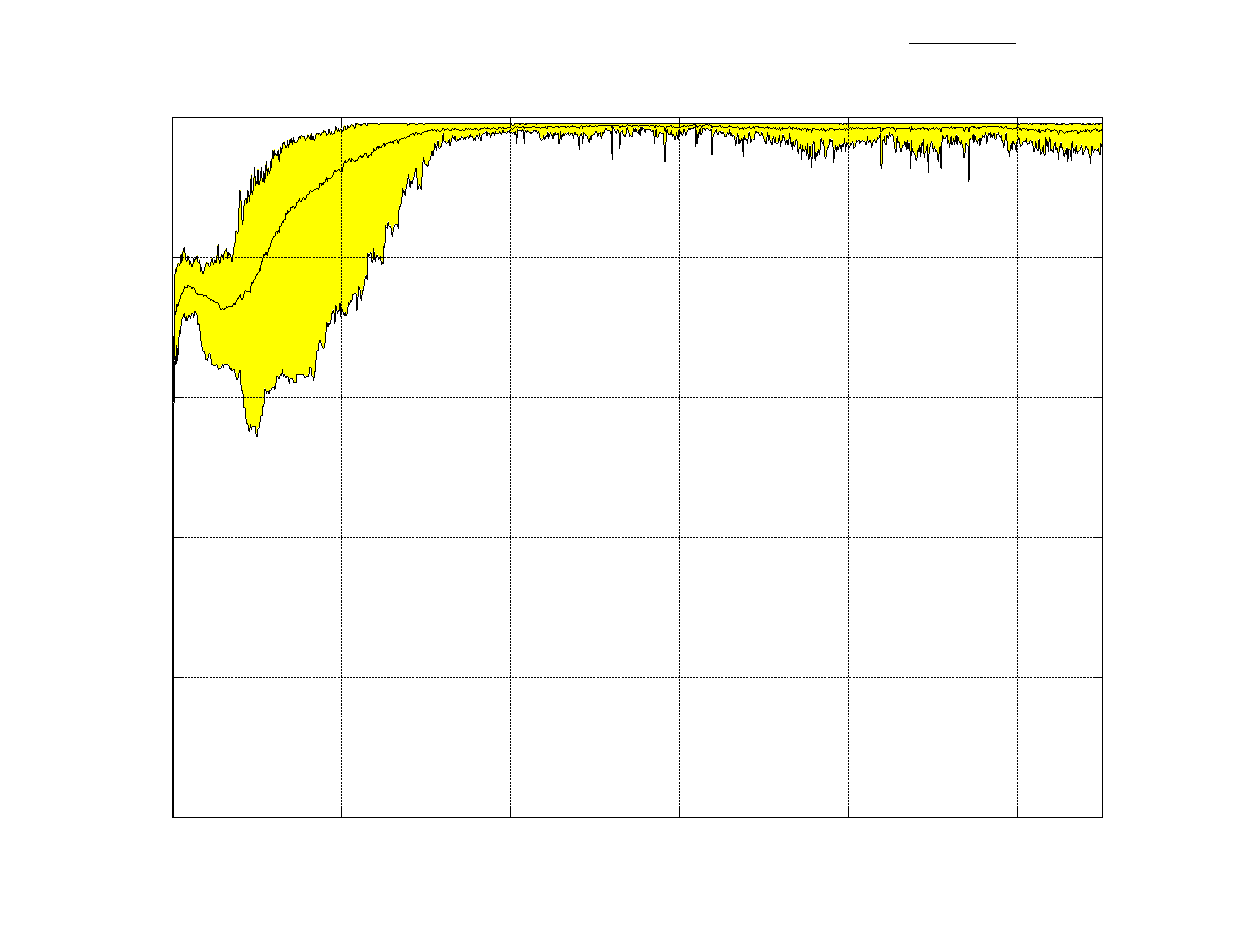
\includegraphics{images/artificial/gmlaslcs0/adder7_24Macc.eps}}%
    \gplfronttext
  \end{picture}%
\endgroup
}
  	\put(-240,60){\rotatebox{90}{$Accuracy$}}
 	\scalebox{0.8}{\put(-180,0){\rotatebox{0}{$iterations$}}}  
  	\end{minipage}
  \begin{minipage}[b]{0.5\linewidth}
  	\centering
  	\scalebox{0.42}{\Large% GNUPLOT: LaTeX picture with Postscript
\begingroup
  \makeatletter
  \providecommand\color[2][]{%
    \GenericError{(gnuplot) \space\space\space\@spaces}{%
      Package color not loaded in conjunction with
      terminal option `colourtext'%
    }{See the gnuplot documentation for explanation.%
    }{Either use 'blacktext' in gnuplot or load the package
      color.sty in LaTeX.}%
    \renewcommand\color[2][]{}%
  }%
  \providecommand\includegraphics[2][]{%
    \GenericError{(gnuplot) \space\space\space\@spaces}{%
      Package graphicx or graphics not loaded%
    }{See the gnuplot documentation for explanation.%
    }{The gnuplot epslatex terminal needs graphicx.sty or graphics.sty.}%
    \renewcommand\includegraphics[2][]{}%
  }%
  \providecommand\rotatebox[2]{#2}%
  \@ifundefined{ifGPcolor}{%
    \newif\ifGPcolor
    \GPcolorfalse
  }{}%
  \@ifundefined{ifGPblacktext}{%
    \newif\ifGPblacktext
    \GPblacktexttrue
  }{}%
  % define a \g@addto@macro without @ in the name:
  \let\gplgaddtomacro\g@addto@macro
  % define empty templates for all commands taking text:
  \gdef\gplbacktext{}%
  \gdef\gplfronttext{}%
  \makeatother
  \ifGPblacktext
    % no textcolor at all
    \def\colorrgb#1{}%
    \def\colorgray#1{}%
  \else
    % gray or color?
    \ifGPcolor
      \def\colorrgb#1{\color[rgb]{#1}}%
      \def\colorgray#1{\color[gray]{#1}}%
      \expandafter\def\csname LTw\endcsname{\color{white}}%
      \expandafter\def\csname LTb\endcsname{\color{black}}%
      \expandafter\def\csname LTa\endcsname{\color{black}}%
      \expandafter\def\csname LT0\endcsname{\color[rgb]{1,0,0}}%
      \expandafter\def\csname LT1\endcsname{\color[rgb]{0,1,0}}%
      \expandafter\def\csname LT2\endcsname{\color[rgb]{0,0,1}}%
      \expandafter\def\csname LT3\endcsname{\color[rgb]{1,0,1}}%
      \expandafter\def\csname LT4\endcsname{\color[rgb]{0,1,1}}%
      \expandafter\def\csname LT5\endcsname{\color[rgb]{1,1,0}}%
      \expandafter\def\csname LT6\endcsname{\color[rgb]{0,0,0}}%
      \expandafter\def\csname LT7\endcsname{\color[rgb]{1,0.3,0}}%
      \expandafter\def\csname LT8\endcsname{\color[rgb]{0.5,0.5,0.5}}%
    \else
      % gray
      \def\colorrgb#1{\color{black}}%
      \def\colorgray#1{\color[gray]{#1}}%
      \expandafter\def\csname LTw\endcsname{\color{white}}%
      \expandafter\def\csname LTb\endcsname{\color{black}}%
      \expandafter\def\csname LTa\endcsname{\color{black}}%
      \expandafter\def\csname LT0\endcsname{\color{black}}%
      \expandafter\def\csname LT1\endcsname{\color{black}}%
      \expandafter\def\csname LT2\endcsname{\color{black}}%
      \expandafter\def\csname LT3\endcsname{\color{black}}%
      \expandafter\def\csname LT4\endcsname{\color{black}}%
      \expandafter\def\csname LT5\endcsname{\color{black}}%
      \expandafter\def\csname LT6\endcsname{\color{black}}%
      \expandafter\def\csname LT7\endcsname{\color{black}}%
      \expandafter\def\csname LT8\endcsname{\color{black}}%
    \fi
  \fi
  \setlength{\unitlength}{0.0500bp}%
  \begin{picture}(11520.00,8640.00)%
    \gplgaddtomacro\gplbacktext{%
    }%
    \gplgaddtomacro\gplfronttext{%
      \csname LTb\endcsname%
      \put(8689,8377){\makebox(0,0)[r]{\strut{}$GMl-ASLCS_{\:0M} \: mean \: exact \: match \: in \: adder_7^{24}$}}%
      \colorrgb{0.00,0.00,0.00}%
      \put(1257,950){\makebox(0,0)[r]{\strut{}$0$}}%
      \colorrgb{0.00,0.00,0.00}%
      \put(1257,2294){\makebox(0,0)[r]{\strut{}$0.2$}}%
      \colorrgb{0.00,0.00,0.00}%
      \put(1257,3637){\makebox(0,0)[r]{\strut{}$0.4$}}%
      \colorrgb{0.00,0.00,0.00}%
      \put(1257,4981){\makebox(0,0)[r]{\strut{}$0.6$}}%
      \colorrgb{0.00,0.00,0.00}%
      \put(1257,6324){\makebox(0,0)[r]{\strut{}$0.8$}}%
      \colorrgb{0.00,0.00,0.00}%
      \put(1257,7668){\makebox(0,0)[r]{\strut{}$1$}}%
      \colorrgb{0.00,0.00,0.00}%
      \put(1497,550){\makebox(0,0){\strut{}$0$}}%
      \colorrgb{0.00,0.00,0.00}%
      \put(3120,550){\makebox(0,0){\strut{}$200$}}%
      \colorrgb{0.00,0.00,0.00}%
      \put(4743,550){\makebox(0,0){\strut{}$400$}}%
      \colorrgb{0.00,0.00,0.00}%
      \put(6366,550){\makebox(0,0){\strut{}$600$}}%
      \colorrgb{0.00,0.00,0.00}%
      \put(7989,550){\makebox(0,0){\strut{}$800$}}%
      \colorrgb{0.00,0.00,0.00}%
      \put(9612,550){\makebox(0,0){\strut{}$1000$}}%
    }%
    \gplbacktext
    \put(0,0){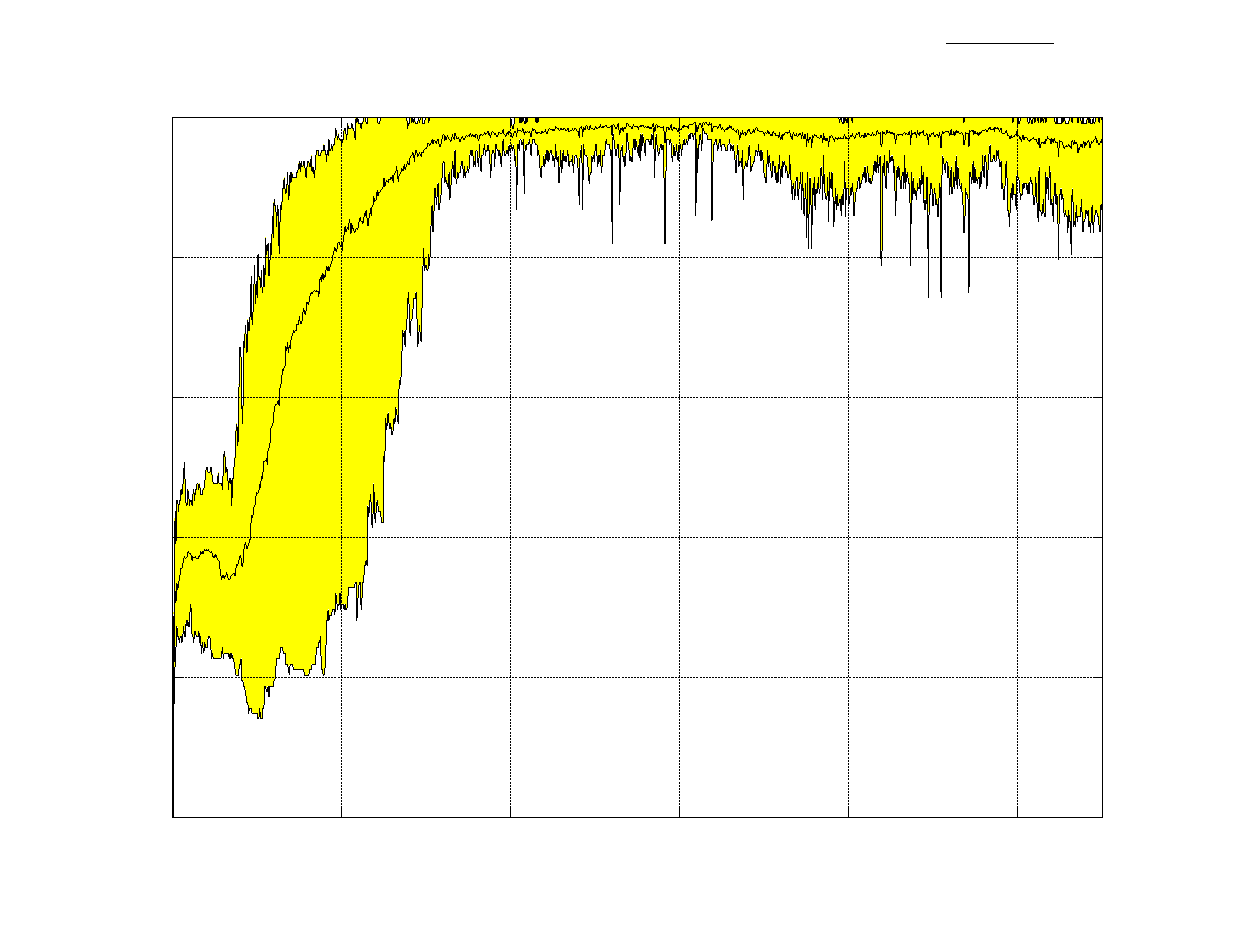
\includegraphics{./images/artificial/gmlaslcs0/adder7_24Mex.eps}}%
    \gplfronttext
  \end{picture}%
\endgroup
}
  	\put(-240,60){\rotatebox{90}{$Exact \: Match$}}
  	\scalebox{0.8}{\put(-180,0){\rotatebox{0}{$iterations$}}}  
  \end{minipage}
\end{figure}

\begin{figure}[ht]
  \caption{Διαγράμματα χαρτογράφησης $adder_{7}^{24}$ του GMl-ASLCS$_{\:0C}$.}
  \label{fig:gmlaslcs0Cadder7_24}
  \begin{minipage}[b]{0.5\linewidth}
  	\centering
  	\scalebox{0.42}{\Large% GNUPLOT: LaTeX picture with Postscript
\begingroup
  \makeatletter
  \providecommand\color[2][]{%
    \GenericError{(gnuplot) \space\space\space\@spaces}{%
      Package color not loaded in conjunction with
      terminal option `colourtext'%
    }{See the gnuplot documentation for explanation.%
    }{Either use 'blacktext' in gnuplot or load the package
      color.sty in LaTeX.}%
    \renewcommand\color[2][]{}%
  }%
  \providecommand\includegraphics[2][]{%
    \GenericError{(gnuplot) \space\space\space\@spaces}{%
      Package graphicx or graphics not loaded%
    }{See the gnuplot documentation for explanation.%
    }{The gnuplot epslatex terminal needs graphicx.sty or graphics.sty.}%
    \renewcommand\includegraphics[2][]{}%
  }%
  \providecommand\rotatebox[2]{#2}%
  \@ifundefined{ifGPcolor}{%
    \newif\ifGPcolor
    \GPcolorfalse
  }{}%
  \@ifundefined{ifGPblacktext}{%
    \newif\ifGPblacktext
    \GPblacktexttrue
  }{}%
  % define a \g@addto@macro without @ in the name:
  \let\gplgaddtomacro\g@addto@macro
  % define empty templates for all commands taking text:
  \gdef\gplbacktext{}%
  \gdef\gplfronttext{}%
  \makeatother
  \ifGPblacktext
    % no textcolor at all
    \def\colorrgb#1{}%
    \def\colorgray#1{}%
  \else
    % gray or color?
    \ifGPcolor
      \def\colorrgb#1{\color[rgb]{#1}}%
      \def\colorgray#1{\color[gray]{#1}}%
      \expandafter\def\csname LTw\endcsname{\color{white}}%
      \expandafter\def\csname LTb\endcsname{\color{black}}%
      \expandafter\def\csname LTa\endcsname{\color{black}}%
      \expandafter\def\csname LT0\endcsname{\color[rgb]{1,0,0}}%
      \expandafter\def\csname LT1\endcsname{\color[rgb]{0,1,0}}%
      \expandafter\def\csname LT2\endcsname{\color[rgb]{0,0,1}}%
      \expandafter\def\csname LT3\endcsname{\color[rgb]{1,0,1}}%
      \expandafter\def\csname LT4\endcsname{\color[rgb]{0,1,1}}%
      \expandafter\def\csname LT5\endcsname{\color[rgb]{1,1,0}}%
      \expandafter\def\csname LT6\endcsname{\color[rgb]{0,0,0}}%
      \expandafter\def\csname LT7\endcsname{\color[rgb]{1,0.3,0}}%
      \expandafter\def\csname LT8\endcsname{\color[rgb]{0.5,0.5,0.5}}%
    \else
      % gray
      \def\colorrgb#1{\color{black}}%
      \def\colorgray#1{\color[gray]{#1}}%
      \expandafter\def\csname LTw\endcsname{\color{white}}%
      \expandafter\def\csname LTb\endcsname{\color{black}}%
      \expandafter\def\csname LTa\endcsname{\color{black}}%
      \expandafter\def\csname LT0\endcsname{\color{black}}%
      \expandafter\def\csname LT1\endcsname{\color{black}}%
      \expandafter\def\csname LT2\endcsname{\color{black}}%
      \expandafter\def\csname LT3\endcsname{\color{black}}%
      \expandafter\def\csname LT4\endcsname{\color{black}}%
      \expandafter\def\csname LT5\endcsname{\color{black}}%
      \expandafter\def\csname LT6\endcsname{\color{black}}%
      \expandafter\def\csname LT7\endcsname{\color{black}}%
      \expandafter\def\csname LT8\endcsname{\color{black}}%
    \fi
  \fi
  \setlength{\unitlength}{0.0500bp}%
  \begin{picture}(11520.00,8640.00)%
    \gplgaddtomacro\gplbacktext{%
    }%
    \gplgaddtomacro\gplfronttext{%
      \csname LTb\endcsname%
      \put(8209,8377){\makebox(0,0)[r]{\strut{}$GMl-ASLCS_{\:0C} \: mean \: accuracy \: in \: adder_7^{24}$}}%
      \colorrgb{0.00,0.00,0.00}%
      \put(1257,950){\makebox(0,0)[r]{\strut{}$0$}}%
      \colorrgb{0.00,0.00,0.00}%
      \put(1257,2294){\makebox(0,0)[r]{\strut{}$0.2$}}%
      \colorrgb{0.00,0.00,0.00}%
      \put(1257,3637){\makebox(0,0)[r]{\strut{}$0.4$}}%
      \colorrgb{0.00,0.00,0.00}%
      \put(1257,4981){\makebox(0,0)[r]{\strut{}$0.6$}}%
      \colorrgb{0.00,0.00,0.00}%
      \put(1257,6324){\makebox(0,0)[r]{\strut{}$0.8$}}%
      \colorrgb{0.00,0.00,0.00}%
      \put(1257,7668){\makebox(0,0)[r]{\strut{}$1$}}%
      \colorrgb{0.00,0.00,0.00}%
      \put(1497,550){\makebox(0,0){\strut{}$0$}}%
      \colorrgb{0.00,0.00,0.00}%
      \put(3120,550){\makebox(0,0){\strut{}$200$}}%
      \colorrgb{0.00,0.00,0.00}%
      \put(4743,550){\makebox(0,0){\strut{}$400$}}%
      \colorrgb{0.00,0.00,0.00}%
      \put(6366,550){\makebox(0,0){\strut{}$600$}}%
      \colorrgb{0.00,0.00,0.00}%
      \put(7989,550){\makebox(0,0){\strut{}$800$}}%
      \colorrgb{0.00,0.00,0.00}%
      \put(9612,550){\makebox(0,0){\strut{}$1000$}}%
    }%
    \gplbacktext
    \put(0,0){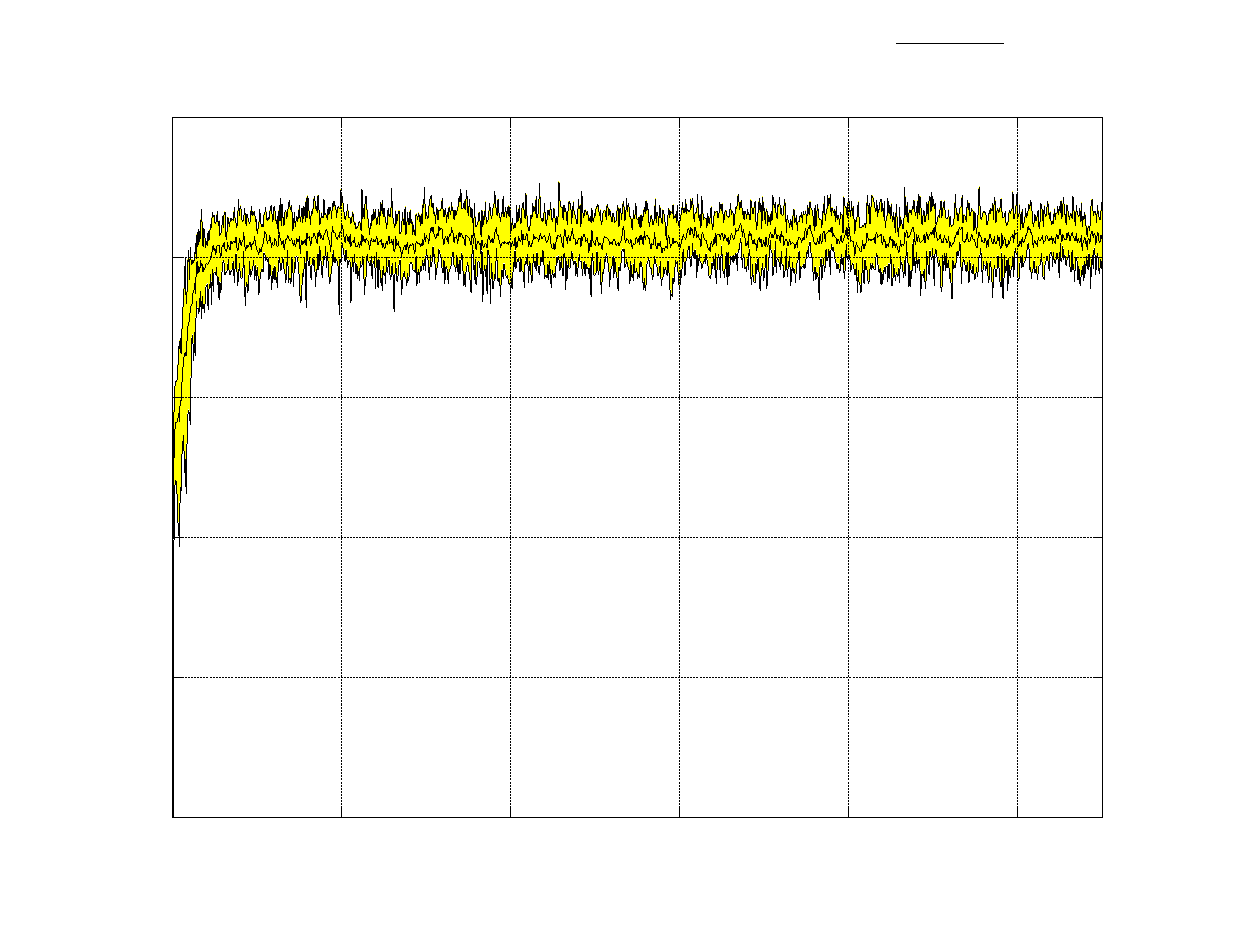
\includegraphics{./images/artificial/gmlaslcs0/adder7_24Cacc.eps}}%
    \gplfronttext
  \end{picture}%
\endgroup
}
  	\put(-240,60){\rotatebox{90}{$Accuracy$}}
 	\scalebox{0.8}{\put(-180,0){\rotatebox{0}{$iterations$}}}  
  	\end{minipage}
  \begin{minipage}[b]{0.5\linewidth}
  	\centering
  	\scalebox{0.42}{\Large% GNUPLOT: LaTeX picture with Postscript
\begingroup
  \makeatletter
  \providecommand\color[2][]{%
    \GenericError{(gnuplot) \space\space\space\@spaces}{%
      Package color not loaded in conjunction with
      terminal option `colourtext'%
    }{See the gnuplot documentation for explanation.%
    }{Either use 'blacktext' in gnuplot or load the package
      color.sty in LaTeX.}%
    \renewcommand\color[2][]{}%
  }%
  \providecommand\includegraphics[2][]{%
    \GenericError{(gnuplot) \space\space\space\@spaces}{%
      Package graphicx or graphics not loaded%
    }{See the gnuplot documentation for explanation.%
    }{The gnuplot epslatex terminal needs graphicx.sty or graphics.sty.}%
    \renewcommand\includegraphics[2][]{}%
  }%
  \providecommand\rotatebox[2]{#2}%
  \@ifundefined{ifGPcolor}{%
    \newif\ifGPcolor
    \GPcolorfalse
  }{}%
  \@ifundefined{ifGPblacktext}{%
    \newif\ifGPblacktext
    \GPblacktexttrue
  }{}%
  % define a \g@addto@macro without @ in the name:
  \let\gplgaddtomacro\g@addto@macro
  % define empty templates for all commands taking text:
  \gdef\gplbacktext{}%
  \gdef\gplfronttext{}%
  \makeatother
  \ifGPblacktext
    % no textcolor at all
    \def\colorrgb#1{}%
    \def\colorgray#1{}%
  \else
    % gray or color?
    \ifGPcolor
      \def\colorrgb#1{\color[rgb]{#1}}%
      \def\colorgray#1{\color[gray]{#1}}%
      \expandafter\def\csname LTw\endcsname{\color{white}}%
      \expandafter\def\csname LTb\endcsname{\color{black}}%
      \expandafter\def\csname LTa\endcsname{\color{black}}%
      \expandafter\def\csname LT0\endcsname{\color[rgb]{1,0,0}}%
      \expandafter\def\csname LT1\endcsname{\color[rgb]{0,1,0}}%
      \expandafter\def\csname LT2\endcsname{\color[rgb]{0,0,1}}%
      \expandafter\def\csname LT3\endcsname{\color[rgb]{1,0,1}}%
      \expandafter\def\csname LT4\endcsname{\color[rgb]{0,1,1}}%
      \expandafter\def\csname LT5\endcsname{\color[rgb]{1,1,0}}%
      \expandafter\def\csname LT6\endcsname{\color[rgb]{0,0,0}}%
      \expandafter\def\csname LT7\endcsname{\color[rgb]{1,0.3,0}}%
      \expandafter\def\csname LT8\endcsname{\color[rgb]{0.5,0.5,0.5}}%
    \else
      % gray
      \def\colorrgb#1{\color{black}}%
      \def\colorgray#1{\color[gray]{#1}}%
      \expandafter\def\csname LTw\endcsname{\color{white}}%
      \expandafter\def\csname LTb\endcsname{\color{black}}%
      \expandafter\def\csname LTa\endcsname{\color{black}}%
      \expandafter\def\csname LT0\endcsname{\color{black}}%
      \expandafter\def\csname LT1\endcsname{\color{black}}%
      \expandafter\def\csname LT2\endcsname{\color{black}}%
      \expandafter\def\csname LT3\endcsname{\color{black}}%
      \expandafter\def\csname LT4\endcsname{\color{black}}%
      \expandafter\def\csname LT5\endcsname{\color{black}}%
      \expandafter\def\csname LT6\endcsname{\color{black}}%
      \expandafter\def\csname LT7\endcsname{\color{black}}%
      \expandafter\def\csname LT8\endcsname{\color{black}}%
    \fi
  \fi
  \setlength{\unitlength}{0.0500bp}%
  \begin{picture}(11520.00,8640.00)%
    \gplgaddtomacro\gplbacktext{%
    }%
    \gplgaddtomacro\gplfronttext{%
      \csname LTb\endcsname%
      \put(8569,8377){\makebox(0,0)[r]{\strut{}$GMl-ASLCS_{\:0C} \: mean \: exact \: match \: in \: adder_7^{24}$}}%
      \colorrgb{0.00,0.00,0.00}%
      \put(1257,950){\makebox(0,0)[r]{\strut{}$0$}}%
      \colorrgb{0.00,0.00,0.00}%
      \put(1257,1790){\makebox(0,0)[r]{\strut{}$0.1$}}%
      \colorrgb{0.00,0.00,0.00}%
      \put(1257,2630){\makebox(0,0)[r]{\strut{}$0.2$}}%
      \colorrgb{0.00,0.00,0.00}%
      \put(1257,3469){\makebox(0,0)[r]{\strut{}$0.3$}}%
      \colorrgb{0.00,0.00,0.00}%
      \put(1257,4309){\makebox(0,0)[r]{\strut{}$0.4$}}%
      \colorrgb{0.00,0.00,0.00}%
      \put(1257,5149){\makebox(0,0)[r]{\strut{}$0.5$}}%
      \colorrgb{0.00,0.00,0.00}%
      \put(1257,5988){\makebox(0,0)[r]{\strut{}$0.6$}}%
      \colorrgb{0.00,0.00,0.00}%
      \put(1257,6828){\makebox(0,0)[r]{\strut{}$0.7$}}%
      \colorrgb{0.00,0.00,0.00}%
      \put(1257,7668){\makebox(0,0)[r]{\strut{}$0.8$}}%
      \colorrgb{0.00,0.00,0.00}%
      \put(1497,550){\makebox(0,0){\strut{}$0$}}%
      \colorrgb{0.00,0.00,0.00}%
      \put(3120,550){\makebox(0,0){\strut{}$200$}}%
      \colorrgb{0.00,0.00,0.00}%
      \put(4743,550){\makebox(0,0){\strut{}$400$}}%
      \colorrgb{0.00,0.00,0.00}%
      \put(6366,550){\makebox(0,0){\strut{}$600$}}%
      \colorrgb{0.00,0.00,0.00}%
      \put(7989,550){\makebox(0,0){\strut{}$800$}}%
      \colorrgb{0.00,0.00,0.00}%
      \put(9612,550){\makebox(0,0){\strut{}$1000$}}%
    }%
    \gplbacktext
    \put(0,0){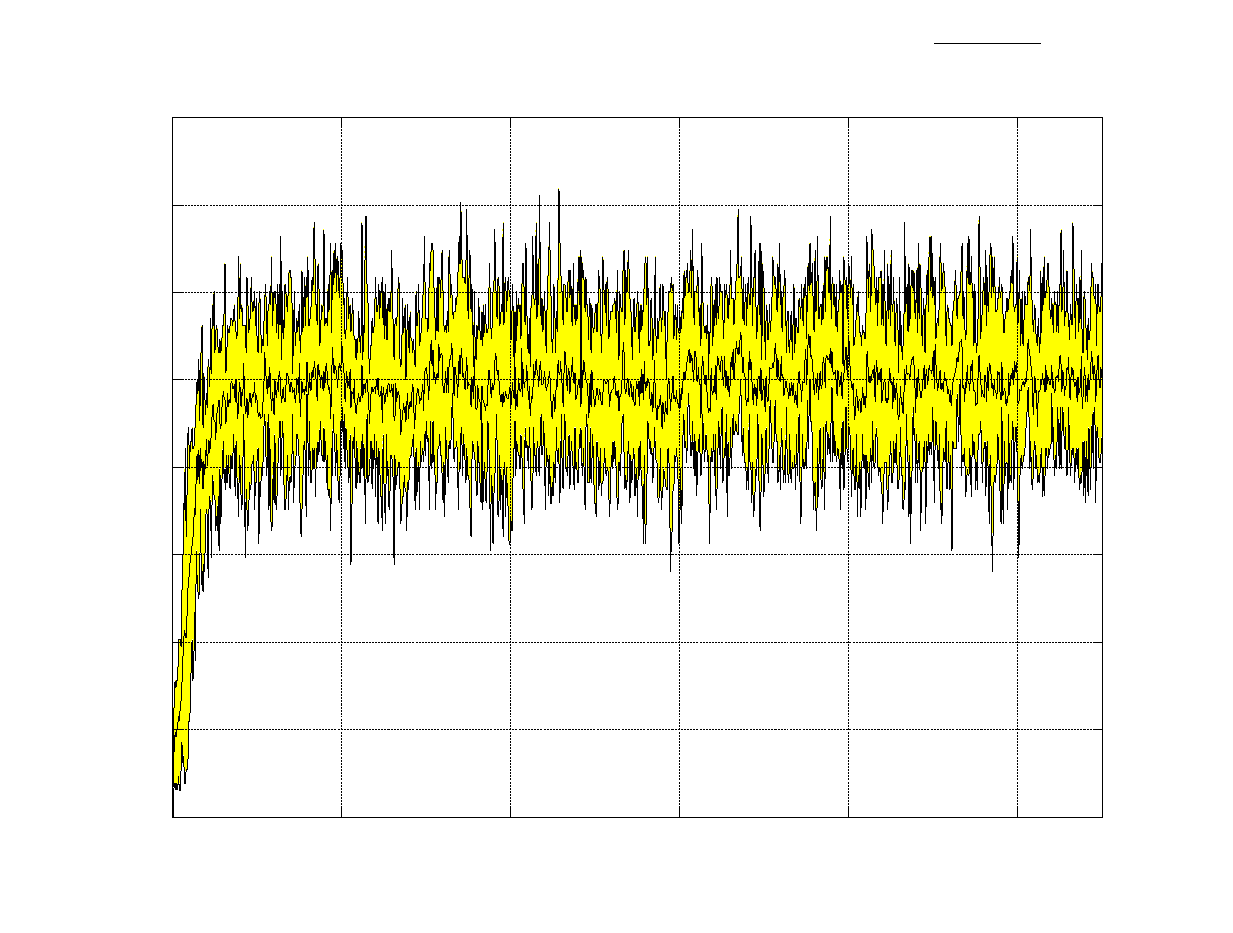
\includegraphics{./images/artificial/gmlaslcs0/adder7_24Cex.eps}}%
    \gplfronttext
  \end{picture}%
\endgroup
}
  	\put(-240,60){\rotatebox{90}{$Exact \: Match$}}
  	\scalebox{0.8}{\put(-180,0){\rotatebox{0}{$iterations$}}}  
  \end{minipage}
\end{figure}


Λόγω της μεγάλης παρουσίας αδιαφοριών στους κανόνες του ΧΒΑ και του γεγονότος ότι δεν τιμωρούνται οι αδιαφορίες στο τμήμα της απόφασης των κανόνων, οι τροποποιήσεις της λειτουργίας διαγραφής και του τελεστή διασταύρωσης κάνουν τους GMl-ASLCS$_{\:0D}$ και GMl-ASLCS$_{\:0GA}$ να καταφέρνουν όχι μόνο να συγκλίνουν προς τις βέλτιστες λύσεις, σε αντίθεση με τον GMl-ASLCS$_{\:0}$, αλλά και να το κάνουν σε λιγότερες από $600$ επαναλήψεις. Και σε αυτό το σύνολο δεδομένων, όπως και στο $adder_{7}^{3}$, παρατηρούμε την πτώση (δηλαδή τη σημαντική βελτίωση) των ελάχιστων τιμών των μετρικών της Ακρίβειας και της Ακριβούς Ορθότητας στον GMl-ASLCS$_{\:0GA}$. 

Ο GMl-ASLCS$_{\:0M}$ καταφέρνει να συγκλίνει και αυτός γρηγορότερα από τον GMl-ASLCS$_{\:0}$, και μάλιστα μέσα σε $400$ επαναλήψεις, βελτιώνοντας ταυτόχρονα τις ελάχιστες τιμές των μετρικών αξιολόγησης που χρησιμοποιήθηκαν. Καταφέρνει επίσης να αυξήσει τη μέση κάλυψη δειγμάτων από τους κανόνες του πληθυσμού του, εκμεταλλευόμενος και εδώ την παρουσία αδιαφοριών στο τμήμα απόφασης των κανόνων του ΧΒΑ.

Τέλος, ο GMl-ASLCS$_{\:0C}$ αποτυγχάνει και εδώ να βελτιώσει με το χρόνο τις λύσεις που εξελίσσει, καθώς παρατηρείται η ίδια συμπεριφορά όπως και στα σύνολα $mlIdentity_{7}$ και $adder_{7}^{3}$. Ενδιαφέρον είναι ότι η πολυκατηγορική πληθικότητα του συνόλου $adder_{7}^{24}$ έχει την ίδια τιμή με αυτή των δύο παραπάνω συνόλων. 




\subsection{Αποτίμηση της επίδρασης της τροποποιημένης λειτουργίας διαγραφής και του τελεστή διασταύρωσης Δύο Τμημάτων}
Η συμπεριφορά των GMl-ASLCS$_{\:0D}$ και GMl-ASLCS$_{\:0GA}$, σε γενικές γραμμές, συνάδει με τα αποτελέσματα που αναμέναμε να επιφέρει η τροποποίηση της λειτουργίας διαγραφής και του τελεστή διασταύρωσης, αντίστοιχα, με βάση τους λόγους για την τροποποίησή τους. Γενικότερα, παρατηρούμε την ταχύτερη σύγκλιση σε όλα τα σύνολα δεδομένων για όλες τις μετρικές αξιολόγησης των μοντέλων που αναπτύσσουν οι GMl-ASLCS$_{\:0D}$ και GMl-ASLCS$_{\:0GA}$, την αύξηση των επιδόσεών τους, και την ταυτόχρονη μείωση του εύρους των χρησιμοποιούμενων μετρικών και στα δέκα πειράματα. 

Όσον αφορά στην τροποποίηση της λειτουργίας διαγραφής, δεδομένης της ισοτιμίας αδιαφορίας και συμφωνίας για τις ετικέτες ως προς τη μεταβολή του αριθμού ορθών κατηγοριοποίησεων, το πρώτο σκέλος της Εξ. \ref{eq:deletionFormula}, που περιλαμβάνει τον τρόπο διαγραφής για τους κανόνες κάτω από το κατώφλι εμπειρίας $\theta_{del}$, δείχνει ότι μπορεί να επιτύχει αξιόλογο διαχωρισμό των κανόνων μέσα στο σύνολο νέων κανόνων με χαμηλή τιμή καταλληλότητας, αλλά και σε σχέση με το σύνολο των κανόνων με $experience \geq \theta_{del}$, λόγω της πιο άμεσης αφαίρεσης κανόνων χαμηλής ποιότητας από τον πληθυσμό, σε σχέση με τον GMl-ASLCS$_{\:0}$.

Όσον αφορά στην τροποποίηση του τελεστή διασταύρωσης, η Διασταύρωση Δύο Τμημάτων επιβεβαιώνεται ως μία αξιόπιστη και αποτελεσματικότερη εναλλακτική της Διασταύρωσης Ενός Σημείου, ιδιαίτερα μάλιστα στα πλαίσια της συνιστώσας ενημέρωσης του GMl-ASLCS$_{\:0}$, όπου η παρουσία αδιαφοριών στα τμήματα απόφασης των κανόνων είναι εντονότερη, λόγω της ισότιμης αντιμετώπισης αδιαφοριών και σαφών αποφάσεων υπέρ ετικετών. Εκτός της ορθότερης εναλλαγής αποφάσεων ανάμεσα στους κανόνες που διασταυρώνονται, και συνεπώς της εξέλιξης ακριβέστερων κανόνων, η μέθοδος Διασταύρωσης Δύο Τμημάτων είναι και ανεξάρτητη από την πολυκατηγορική πυκνότητα των συνόλων δεδομένων.


 
\subsection{Αποτίμηση της επίδρασης της διαγραφής κανόνων με κριτήρια πάνω στα Match Sets}
Από τη συμπεριφορά του GMl-ASLCS$_{\:0M}$ στα τέσσερα τεχνητά σύνολα δεδομένων συμπεραίνουμε πως η λειτουργία της διαγραφής κανόνων από τα Match Set είναι εύρωστη και αποτελεσματική ως προς την αύξηση του μέσου ποσοστού κάλυψης δειγμάτων, ενώ ταυτόχρονα δεν επηρεάζει με αρνητικό τρόπο την Ακρίβεια. Σε πιθανό συνδυασμό με την υλοποίηση της τιμωρίας κανόνων που αδιαφορούν για ετικέτες, θα περιμέναμε την απόσβεση όποιου φαινομένου αποσταθεροποίησης του πληθυσμού και των χαρακτηριστικών των κανόνων του, όπως φάνηκε από το γράφημα του Σχήματος \ref{fig:gmlaslcs0MPosition7}, του μέσου ποσοστού εύρεσης του ΧΒΑ του προβλήματος $mlPosition_{7}$ και τη συνολική βελτίωση της ευρωστίας της μεθόδου, αλλά και του αλγορίθμου.

\subsection{Αποτίμηση της επίδρασης της έκπτωσης του αριθμού ορθών κατηγοριοποιήσεων για τους κανόνες που αδιαφορούν για ετικέτες}

Το εύρος της Ακρίβειας των λύσεων που εξελίσσει ο GMl-ASLCS$_{\:0C}$ μειώνεται σε σχέση με αυτό των λύσεων του GMl-ASLCS$_{\:0}$, κάνοντας τον GMl-ASLCS$_{\:0C}$ να υπολείπεται σε επιδόσεις, εμφανίζοντας στάσιμη συμπεριφορά όταν η πολυκατηγορική πυκνότητα του συνόλου εκπαίδευσης εμφανίζει υψηλές τιμές. Αυτό είναι κάτι αναμενόμενο, καθώς, μειώνονται μεν με το πέρασμα των επαναλήψεων οι αδιαφορίες στα τμήματα απόφασης των κανόνων, λόγω της τιμωρίας της καταλληλότητάς τους, η εναλλαγή όμως ολόκληρων τμημάτων των αποφάσεων τους μέσω της Διασταύρωσης Ενός Σημείου λειτουργεί αποτρεπτικά προς την εύρεση νέων, βελτιωμένων λύσεων και, συνεπώς, προς την αύξηση των επιδόσεων του ΜαΣΤ. Εν τέλει, το ΜαΣΤ αναλώνεται στην “εύρεση" των ίδιων λύσεων, ενώ παράλληλα ο συνδυασμός του παραπάνω τελεστή διασταύρωσης και της έκπτωσης της ακρίβειας των κανόνων είναι δυνατόν να λειτουργήσει με τέτοιο τρόπο που να μην αυξάνει στον επιθυμητό βαθμό τη μέση κάλυψη των δειγμάτων από τους κανόνες του πληθυσμού. Παρ' όλα αυτά, ο συνδυασμός αυτής της λειτουργίας, με τη Διασταύρωση Δύο Τμημάτων που είναι ανεξάρτητη από την πολυκατηγορική πυκνότητα των συνόλων εκπαίδευσης, αλλά και τη διαγραφή κανόνων από τα Match Sets που διαγράφει τους κανόνες χαμηλής καταλληλότητας στα χαμηλότερα επίπεδα κάλυψης, αναμένουμε ότι θα συνηγορήσουν υπέρ της αποτελμάτωσης των λύσεων που εξελίσσει ο GMl-ASLCS.





%-------------------------------GMl-ASLCS-------------------------------%




\section{Πολυκατηγορική Ταξινόμηση με τον GMl-ASLCS}




\begin{figure}[ht]
  \caption{Διαγράμματα χαρτογράφησης $mlPosition_{7}$ του GMl-ASLCS.}
  \label{fig:gmlaslcsPosition7}
  \centering
  \scalebox{0.49}{\Large% GNUPLOT: LaTeX picture with Postscript
\begingroup
  \makeatletter
  \providecommand\color[2][]{%
    \GenericError{(gnuplot) \space\space\space\@spaces}{%
      Package color not loaded in conjunction with
      terminal option `colourtext'%
    }{See the gnuplot documentation for explanation.%
    }{Either use 'blacktext' in gnuplot or load the package
      color.sty in LaTeX.}%
    \renewcommand\color[2][]{}%
  }%
  \providecommand\includegraphics[2][]{%
    \GenericError{(gnuplot) \space\space\space\@spaces}{%
      Package graphicx or graphics not loaded%
    }{See the gnuplot documentation for explanation.%
    }{The gnuplot epslatex terminal needs graphicx.sty or graphics.sty.}%
    \renewcommand\includegraphics[2][]{}%
  }%
  \providecommand\rotatebox[2]{#2}%
  \@ifundefined{ifGPcolor}{%
    \newif\ifGPcolor
    \GPcolorfalse
  }{}%
  \@ifundefined{ifGPblacktext}{%
    \newif\ifGPblacktext
    \GPblacktexttrue
  }{}%
  % define a \g@addto@macro without @ in the name:
  \let\gplgaddtomacro\g@addto@macro
  % define empty templates for all commands taking text:
  \gdef\gplbacktext{}%
  \gdef\gplfronttext{}%
  \makeatother
  \ifGPblacktext
    % no textcolor at all
    \def\colorrgb#1{}%
    \def\colorgray#1{}%
  \else
    % gray or color?
    \ifGPcolor
      \def\colorrgb#1{\color[rgb]{#1}}%
      \def\colorgray#1{\color[gray]{#1}}%
      \expandafter\def\csname LTw\endcsname{\color{white}}%
      \expandafter\def\csname LTb\endcsname{\color{black}}%
      \expandafter\def\csname LTa\endcsname{\color{black}}%
      \expandafter\def\csname LT0\endcsname{\color[rgb]{1,0,0}}%
      \expandafter\def\csname LT1\endcsname{\color[rgb]{0,1,0}}%
      \expandafter\def\csname LT2\endcsname{\color[rgb]{0,0,1}}%
      \expandafter\def\csname LT3\endcsname{\color[rgb]{1,0,1}}%
      \expandafter\def\csname LT4\endcsname{\color[rgb]{0,1,1}}%
      \expandafter\def\csname LT5\endcsname{\color[rgb]{1,1,0}}%
      \expandafter\def\csname LT6\endcsname{\color[rgb]{0,0,0}}%
      \expandafter\def\csname LT7\endcsname{\color[rgb]{1,0.3,0}}%
      \expandafter\def\csname LT8\endcsname{\color[rgb]{0.5,0.5,0.5}}%
    \else
      % gray
      \def\colorrgb#1{\color{black}}%
      \def\colorgray#1{\color[gray]{#1}}%
      \expandafter\def\csname LTw\endcsname{\color{white}}%
      \expandafter\def\csname LTb\endcsname{\color{black}}%
      \expandafter\def\csname LTa\endcsname{\color{black}}%
      \expandafter\def\csname LT0\endcsname{\color{black}}%
      \expandafter\def\csname LT1\endcsname{\color{black}}%
      \expandafter\def\csname LT2\endcsname{\color{black}}%
      \expandafter\def\csname LT3\endcsname{\color{black}}%
      \expandafter\def\csname LT4\endcsname{\color{black}}%
      \expandafter\def\csname LT5\endcsname{\color{black}}%
      \expandafter\def\csname LT6\endcsname{\color{black}}%
      \expandafter\def\csname LT7\endcsname{\color{black}}%
      \expandafter\def\csname LT8\endcsname{\color{black}}%
    \fi
  \fi
  \setlength{\unitlength}{0.0500bp}%
  \begin{picture}(11520.00,8640.00)%
    \gplgaddtomacro\gplbacktext{%
    }%
    \gplgaddtomacro\gplfronttext{%
      \csname LTb\endcsname%
      \put(8569,8377){\makebox(0,0)[r]{\strut{}$GMl-ASLCS \: mean \: accuracy \: in\:  mlPosition_7$}}%
      \colorrgb{0.00,0.00,0.00}%
      \put(1257,950){\makebox(0,0)[r]{\strut{}$0$}}%
      \colorrgb{0.00,0.00,0.00}%
      \put(1257,2171){\makebox(0,0)[r]{\strut{}$0.2$}}%
      \colorrgb{0.00,0.00,0.00}%
      \put(1257,3393){\makebox(0,0)[r]{\strut{}$0.4$}}%
      \colorrgb{0.00,0.00,0.00}%
      \put(1257,4614){\makebox(0,0)[r]{\strut{}$0.6$}}%
      \colorrgb{0.00,0.00,0.00}%
      \put(1257,5836){\makebox(0,0)[r]{\strut{}$0.8$}}%
      \colorrgb{0.00,0.00,0.00}%
      \put(1257,7057){\makebox(0,0)[r]{\strut{}$1$}}%
      \colorrgb{0.00,0.00,0.00}%
      \put(1497,550){\makebox(0,0){\strut{}$0$}}%
      \colorrgb{0.00,0.00,0.00}%
      \put(3120,550){\makebox(0,0){\strut{}$200$}}%
      \colorrgb{0.00,0.00,0.00}%
      \put(4743,550){\makebox(0,0){\strut{}$400$}}%
      \colorrgb{0.00,0.00,0.00}%
      \put(6366,550){\makebox(0,0){\strut{}$600$}}%
      \colorrgb{0.00,0.00,0.00}%
      \put(7989,550){\makebox(0,0){\strut{}$800$}}%
      \colorrgb{0.00,0.00,0.00}%
      \put(9612,550){\makebox(0,0){\strut{}$1000$}}%
    }%
    \gplbacktext
    \put(0,0){\includegraphics{./images/artificial/gmlaslcs/positionAcc.eps}}%
    \gplfronttext
  \end{picture}%
\endgroup
}
  \put(-285,70){\rotatebox{90}{$Accuracy$}}
  \scalebox{0.8}{\put(-200,0){\rotatebox{0}{$iterations$}}}
  \label{fig:gmlaslcsPositionAcc} 
  
  \centering
  \scalebox{0.49}{\Large% GNUPLOT: LaTeX picture with Postscript
\begingroup
  \makeatletter
  \providecommand\color[2][]{%
    \GenericError{(gnuplot) \space\space\space\@spaces}{%
      Package color not loaded in conjunction with
      terminal option `colourtext'%
    }{See the gnuplot documentation for explanation.%
    }{Either use 'blacktext' in gnuplot or load the package
      color.sty in LaTeX.}%
    \renewcommand\color[2][]{}%
  }%
  \providecommand\includegraphics[2][]{%
    \GenericError{(gnuplot) \space\space\space\@spaces}{%
      Package graphicx or graphics not loaded%
    }{See the gnuplot documentation for explanation.%
    }{The gnuplot epslatex terminal needs graphicx.sty or graphics.sty.}%
    \renewcommand\includegraphics[2][]{}%
  }%
  \providecommand\rotatebox[2]{#2}%
  \@ifundefined{ifGPcolor}{%
    \newif\ifGPcolor
    \GPcolorfalse
  }{}%
  \@ifundefined{ifGPblacktext}{%
    \newif\ifGPblacktext
    \GPblacktexttrue
  }{}%
  % define a \g@addto@macro without @ in the name:
  \let\gplgaddtomacro\g@addto@macro
  % define empty templates for all commands taking text:
  \gdef\gplbacktext{}%
  \gdef\gplfronttext{}%
  \makeatother
  \ifGPblacktext
    % no textcolor at all
    \def\colorrgb#1{}%
    \def\colorgray#1{}%
  \else
    % gray or color?
    \ifGPcolor
      \def\colorrgb#1{\color[rgb]{#1}}%
      \def\colorgray#1{\color[gray]{#1}}%
      \expandafter\def\csname LTw\endcsname{\color{white}}%
      \expandafter\def\csname LTb\endcsname{\color{black}}%
      \expandafter\def\csname LTa\endcsname{\color{black}}%
      \expandafter\def\csname LT0\endcsname{\color[rgb]{1,0,0}}%
      \expandafter\def\csname LT1\endcsname{\color[rgb]{0,1,0}}%
      \expandafter\def\csname LT2\endcsname{\color[rgb]{0,0,1}}%
      \expandafter\def\csname LT3\endcsname{\color[rgb]{1,0,1}}%
      \expandafter\def\csname LT4\endcsname{\color[rgb]{0,1,1}}%
      \expandafter\def\csname LT5\endcsname{\color[rgb]{1,1,0}}%
      \expandafter\def\csname LT6\endcsname{\color[rgb]{0,0,0}}%
      \expandafter\def\csname LT7\endcsname{\color[rgb]{1,0.3,0}}%
      \expandafter\def\csname LT8\endcsname{\color[rgb]{0.5,0.5,0.5}}%
    \else
      % gray
      \def\colorrgb#1{\color{black}}%
      \def\colorgray#1{\color[gray]{#1}}%
      \expandafter\def\csname LTw\endcsname{\color{white}}%
      \expandafter\def\csname LTb\endcsname{\color{black}}%
      \expandafter\def\csname LTa\endcsname{\color{black}}%
      \expandafter\def\csname LT0\endcsname{\color{black}}%
      \expandafter\def\csname LT1\endcsname{\color{black}}%
      \expandafter\def\csname LT2\endcsname{\color{black}}%
      \expandafter\def\csname LT3\endcsname{\color{black}}%
      \expandafter\def\csname LT4\endcsname{\color{black}}%
      \expandafter\def\csname LT5\endcsname{\color{black}}%
      \expandafter\def\csname LT6\endcsname{\color{black}}%
      \expandafter\def\csname LT7\endcsname{\color{black}}%
      \expandafter\def\csname LT8\endcsname{\color{black}}%
    \fi
  \fi
  \setlength{\unitlength}{0.0500bp}%
  \begin{picture}(11520.00,8640.00)%
    \gplgaddtomacro\gplbacktext{%
    }%
    \gplgaddtomacro\gplfronttext{%
      \csname LTb\endcsname%
      \put(8929,8377){\makebox(0,0)[r]{\strut{}$GMl-ASLCS \: mean \: exact \: match \: in\: mlPosition_7$}}%
      \colorrgb{0.00,0.00,0.00}%
      \put(1257,950){\makebox(0,0)[r]{\strut{}$0$}}%
      \colorrgb{0.00,0.00,0.00}%
      \put(1257,2171){\makebox(0,0)[r]{\strut{}$0.2$}}%
      \colorrgb{0.00,0.00,0.00}%
      \put(1257,3393){\makebox(0,0)[r]{\strut{}$0.4$}}%
      \colorrgb{0.00,0.00,0.00}%
      \put(1257,4614){\makebox(0,0)[r]{\strut{}$0.6$}}%
      \colorrgb{0.00,0.00,0.00}%
      \put(1257,5836){\makebox(0,0)[r]{\strut{}$0.8$}}%
      \colorrgb{0.00,0.00,0.00}%
      \put(1257,7057){\makebox(0,0)[r]{\strut{}$1$}}%
      \colorrgb{0.00,0.00,0.00}%
      \put(1497,550){\makebox(0,0){\strut{}$0$}}%
      \colorrgb{0.00,0.00,0.00}%
      \put(3120,550){\makebox(0,0){\strut{}$200$}}%
      \colorrgb{0.00,0.00,0.00}%
      \put(4743,550){\makebox(0,0){\strut{}$400$}}%
      \colorrgb{0.00,0.00,0.00}%
      \put(6366,550){\makebox(0,0){\strut{}$600$}}%
      \colorrgb{0.00,0.00,0.00}%
      \put(7989,550){\makebox(0,0){\strut{}$800$}}%
      \colorrgb{0.00,0.00,0.00}%
      \put(9612,550){\makebox(0,0){\strut{}$1000$}}%
    }%
    \gplbacktext
    \put(0,0){\includegraphics{./images/artificial/gmlaslcs/positionEx.eps}}%
    \gplfronttext
  \end{picture}%
\endgroup
}
  \put(-285,70){\rotatebox{90}{$Exact \: Match$}}
  \scalebox{0.8}{\put(-200,0){\rotatebox{0}{$iterations$}}}
  \label{fig:gmlaslcsPositionEx}  
   
  \centering
  \scalebox{0.49}{\Large% GNUPLOT: LaTeX picture with Postscript
\begingroup
  \makeatletter
  \providecommand\color[2][]{%
    \GenericError{(gnuplot) \space\space\space\@spaces}{%
      Package color not loaded in conjunction with
      terminal option `colourtext'%
    }{See the gnuplot documentation for explanation.%
    }{Either use 'blacktext' in gnuplot or load the package
      color.sty in LaTeX.}%
    \renewcommand\color[2][]{}%
  }%
  \providecommand\includegraphics[2][]{%
    \GenericError{(gnuplot) \space\space\space\@spaces}{%
      Package graphicx or graphics not loaded%
    }{See the gnuplot documentation for explanation.%
    }{The gnuplot epslatex terminal needs graphicx.sty or graphics.sty.}%
    \renewcommand\includegraphics[2][]{}%
  }%
  \providecommand\rotatebox[2]{#2}%
  \@ifundefined{ifGPcolor}{%
    \newif\ifGPcolor
    \GPcolorfalse
  }{}%
  \@ifundefined{ifGPblacktext}{%
    \newif\ifGPblacktext
    \GPblacktexttrue
  }{}%
  % define a \g@addto@macro without @ in the name:
  \let\gplgaddtomacro\g@addto@macro
  % define empty templates for all commands taking text:
  \gdef\gplbacktext{}%
  \gdef\gplfronttext{}%
  \makeatother
  \ifGPblacktext
    % no textcolor at all
    \def\colorrgb#1{}%
    \def\colorgray#1{}%
  \else
    % gray or color?
    \ifGPcolor
      \def\colorrgb#1{\color[rgb]{#1}}%
      \def\colorgray#1{\color[gray]{#1}}%
      \expandafter\def\csname LTw\endcsname{\color{white}}%
      \expandafter\def\csname LTb\endcsname{\color{black}}%
      \expandafter\def\csname LTa\endcsname{\color{black}}%
      \expandafter\def\csname LT0\endcsname{\color[rgb]{1,0,0}}%
      \expandafter\def\csname LT1\endcsname{\color[rgb]{0,1,0}}%
      \expandafter\def\csname LT2\endcsname{\color[rgb]{0,0,1}}%
      \expandafter\def\csname LT3\endcsname{\color[rgb]{1,0,1}}%
      \expandafter\def\csname LT4\endcsname{\color[rgb]{0,1,1}}%
      \expandafter\def\csname LT5\endcsname{\color[rgb]{1,1,0}}%
      \expandafter\def\csname LT6\endcsname{\color[rgb]{0,0,0}}%
      \expandafter\def\csname LT7\endcsname{\color[rgb]{1,0.3,0}}%
      \expandafter\def\csname LT8\endcsname{\color[rgb]{0.5,0.5,0.5}}%
    \else
      % gray
      \def\colorrgb#1{\color{black}}%
      \def\colorgray#1{\color[gray]{#1}}%
      \expandafter\def\csname LTw\endcsname{\color{white}}%
      \expandafter\def\csname LTb\endcsname{\color{black}}%
      \expandafter\def\csname LTa\endcsname{\color{black}}%
      \expandafter\def\csname LT0\endcsname{\color{black}}%
      \expandafter\def\csname LT1\endcsname{\color{black}}%
      \expandafter\def\csname LT2\endcsname{\color{black}}%
      \expandafter\def\csname LT3\endcsname{\color{black}}%
      \expandafter\def\csname LT4\endcsname{\color{black}}%
      \expandafter\def\csname LT5\endcsname{\color{black}}%
      \expandafter\def\csname LT6\endcsname{\color{black}}%
      \expandafter\def\csname LT7\endcsname{\color{black}}%
      \expandafter\def\csname LT8\endcsname{\color{black}}%
    \fi
  \fi
  \setlength{\unitlength}{0.0500bp}%
  \begin{picture}(11520.00,8640.00)%
    \gplgaddtomacro\gplbacktext{%
    }%
    \gplgaddtomacro\gplfronttext{%
      \csname LTb\endcsname%
      \put(9049,8377){\makebox(0,0)[r]{\strut{}$GMl-ASLCS \: mean \: BAM \: coverage \: in\:  mlPosition_7$}}%
      \colorrgb{0.00,0.00,0.00}%
      \put(1257,950){\makebox(0,0)[r]{\strut{}$0$}}%
      \colorrgb{0.00,0.00,0.00}%
      \put(1257,2294){\makebox(0,0)[r]{\strut{}$0.2$}}%
      \colorrgb{0.00,0.00,0.00}%
      \put(1257,3637){\makebox(0,0)[r]{\strut{}$0.4$}}%
      \colorrgb{0.00,0.00,0.00}%
      \put(1257,4981){\makebox(0,0)[r]{\strut{}$0.6$}}%
      \colorrgb{0.00,0.00,0.00}%
      \put(1257,6324){\makebox(0,0)[r]{\strut{}$0.8$}}%
      \colorrgb{0.00,0.00,0.00}%
      \put(1257,7668){\makebox(0,0)[r]{\strut{}$1$}}%
      \colorrgb{0.00,0.00,0.00}%
      \put(1497,550){\makebox(0,0){\strut{}$0$}}%
      \colorrgb{0.00,0.00,0.00}%
      \put(3120,550){\makebox(0,0){\strut{}$200$}}%
      \colorrgb{0.00,0.00,0.00}%
      \put(4743,550){\makebox(0,0){\strut{}$400$}}%
      \colorrgb{0.00,0.00,0.00}%
      \put(6366,550){\makebox(0,0){\strut{}$600$}}%
      \colorrgb{0.00,0.00,0.00}%
      \put(7989,550){\makebox(0,0){\strut{}$800$}}%
      \colorrgb{0.00,0.00,0.00}%
      \put(9612,550){\makebox(0,0){\strut{}$1000$}}%
    }%
    \gplbacktext
    \put(0,0){\includegraphics{./images/artificial/gmlaslcs/positionBAM.eps}}%
    \gplfronttext
  \end{picture}%
\endgroup
}
  \put(-285,80){\rotatebox{90}{$BAM$}}
  \scalebox{0.8}{\put(-200,0){\rotatebox{0}{$iterations$}}}
  \label{fig:gmlaslcsPositionBAM} 
\end{figure}






\begin{figure}[ht]
  \caption{Διαγράμματα χαρτογράφησης $mlIdentity_{7}$ του GMl-ASLCS.}
  \label{fig:gmlaslcsIdentity7}
  \centering
  \scalebox{0.49}{\Large% GNUPLOT: LaTeX picture with Postscript
\begingroup
  \makeatletter
  \providecommand\color[2][]{%
    \GenericError{(gnuplot) \space\space\space\@spaces}{%
      Package color not loaded in conjunction with
      terminal option `colourtext'%
    }{See the gnuplot documentation for explanation.%
    }{Either use 'blacktext' in gnuplot or load the package
      color.sty in LaTeX.}%
    \renewcommand\color[2][]{}%
  }%
  \providecommand\includegraphics[2][]{%
    \GenericError{(gnuplot) \space\space\space\@spaces}{%
      Package graphicx or graphics not loaded%
    }{See the gnuplot documentation for explanation.%
    }{The gnuplot epslatex terminal needs graphicx.sty or graphics.sty.}%
    \renewcommand\includegraphics[2][]{}%
  }%
  \providecommand\rotatebox[2]{#2}%
  \@ifundefined{ifGPcolor}{%
    \newif\ifGPcolor
    \GPcolorfalse
  }{}%
  \@ifundefined{ifGPblacktext}{%
    \newif\ifGPblacktext
    \GPblacktexttrue
  }{}%
  % define a \g@addto@macro without @ in the name:
  \let\gplgaddtomacro\g@addto@macro
  % define empty templates for all commands taking text:
  \gdef\gplbacktext{}%
  \gdef\gplfronttext{}%
  \makeatother
  \ifGPblacktext
    % no textcolor at all
    \def\colorrgb#1{}%
    \def\colorgray#1{}%
  \else
    % gray or color?
    \ifGPcolor
      \def\colorrgb#1{\color[rgb]{#1}}%
      \def\colorgray#1{\color[gray]{#1}}%
      \expandafter\def\csname LTw\endcsname{\color{white}}%
      \expandafter\def\csname LTb\endcsname{\color{black}}%
      \expandafter\def\csname LTa\endcsname{\color{black}}%
      \expandafter\def\csname LT0\endcsname{\color[rgb]{1,0,0}}%
      \expandafter\def\csname LT1\endcsname{\color[rgb]{0,1,0}}%
      \expandafter\def\csname LT2\endcsname{\color[rgb]{0,0,1}}%
      \expandafter\def\csname LT3\endcsname{\color[rgb]{1,0,1}}%
      \expandafter\def\csname LT4\endcsname{\color[rgb]{0,1,1}}%
      \expandafter\def\csname LT5\endcsname{\color[rgb]{1,1,0}}%
      \expandafter\def\csname LT6\endcsname{\color[rgb]{0,0,0}}%
      \expandafter\def\csname LT7\endcsname{\color[rgb]{1,0.3,0}}%
      \expandafter\def\csname LT8\endcsname{\color[rgb]{0.5,0.5,0.5}}%
    \else
      % gray
      \def\colorrgb#1{\color{black}}%
      \def\colorgray#1{\color[gray]{#1}}%
      \expandafter\def\csname LTw\endcsname{\color{white}}%
      \expandafter\def\csname LTb\endcsname{\color{black}}%
      \expandafter\def\csname LTa\endcsname{\color{black}}%
      \expandafter\def\csname LT0\endcsname{\color{black}}%
      \expandafter\def\csname LT1\endcsname{\color{black}}%
      \expandafter\def\csname LT2\endcsname{\color{black}}%
      \expandafter\def\csname LT3\endcsname{\color{black}}%
      \expandafter\def\csname LT4\endcsname{\color{black}}%
      \expandafter\def\csname LT5\endcsname{\color{black}}%
      \expandafter\def\csname LT6\endcsname{\color{black}}%
      \expandafter\def\csname LT7\endcsname{\color{black}}%
      \expandafter\def\csname LT8\endcsname{\color{black}}%
    \fi
  \fi
  \setlength{\unitlength}{0.0500bp}%
  \begin{picture}(11520.00,8640.00)%
    \gplgaddtomacro\gplbacktext{%
    }%
    \gplgaddtomacro\gplfronttext{%
      \csname LTb\endcsname%
      \put(8569,8377){\makebox(0,0)[r]{\strut{}$GMl-ASLCS \: mean \: accuracy\:  in \: mlIdentity_7$}}%
      \colorrgb{0.00,0.00,0.00}%
      \put(1257,950){\makebox(0,0)[r]{\strut{}$0$}}%
      \colorrgb{0.00,0.00,0.00}%
      \put(1257,2171){\makebox(0,0)[r]{\strut{}$0.2$}}%
      \colorrgb{0.00,0.00,0.00}%
      \put(1257,3393){\makebox(0,0)[r]{\strut{}$0.4$}}%
      \colorrgb{0.00,0.00,0.00}%
      \put(1257,4614){\makebox(0,0)[r]{\strut{}$0.6$}}%
      \colorrgb{0.00,0.00,0.00}%
      \put(1257,5836){\makebox(0,0)[r]{\strut{}$0.8$}}%
      \colorrgb{0.00,0.00,0.00}%
      \put(1257,7057){\makebox(0,0)[r]{\strut{}$1$}}%
      \colorrgb{0.00,0.00,0.00}%
      \put(1497,550){\makebox(0,0){\strut{}$0$}}%
      \colorrgb{0.00,0.00,0.00}%
      \put(3120,550){\makebox(0,0){\strut{}$200$}}%
      \colorrgb{0.00,0.00,0.00}%
      \put(4743,550){\makebox(0,0){\strut{}$400$}}%
      \colorrgb{0.00,0.00,0.00}%
      \put(6366,550){\makebox(0,0){\strut{}$600$}}%
      \colorrgb{0.00,0.00,0.00}%
      \put(7989,550){\makebox(0,0){\strut{}$800$}}%
      \colorrgb{0.00,0.00,0.00}%
      \put(9612,550){\makebox(0,0){\strut{}$1000$}}%
    }%
    \gplbacktext
    \put(0,0){\includegraphics{./images/artificial/gmlaslcs/identityAcc.eps}}%
    \gplfronttext
  \end{picture}%
\endgroup
}
  \put(-285,70){\rotatebox{90}{$Accuracy$}}
  \scalebox{0.8}{\put(-200,0){\rotatebox{0}{$iterations$}}}
  \label{fig:gmlaslcsIdentityAcc} 
  
  \centering
  \scalebox{0.49}{\Large% GNUPLOT: LaTeX picture with Postscript
\begingroup
  \makeatletter
  \providecommand\color[2][]{%
    \GenericError{(gnuplot) \space\space\space\@spaces}{%
      Package color not loaded in conjunction with
      terminal option `colourtext'%
    }{See the gnuplot documentation for explanation.%
    }{Either use 'blacktext' in gnuplot or load the package
      color.sty in LaTeX.}%
    \renewcommand\color[2][]{}%
  }%
  \providecommand\includegraphics[2][]{%
    \GenericError{(gnuplot) \space\space\space\@spaces}{%
      Package graphicx or graphics not loaded%
    }{See the gnuplot documentation for explanation.%
    }{The gnuplot epslatex terminal needs graphicx.sty or graphics.sty.}%
    \renewcommand\includegraphics[2][]{}%
  }%
  \providecommand\rotatebox[2]{#2}%
  \@ifundefined{ifGPcolor}{%
    \newif\ifGPcolor
    \GPcolorfalse
  }{}%
  \@ifundefined{ifGPblacktext}{%
    \newif\ifGPblacktext
    \GPblacktexttrue
  }{}%
  % define a \g@addto@macro without @ in the name:
  \let\gplgaddtomacro\g@addto@macro
  % define empty templates for all commands taking text:
  \gdef\gplbacktext{}%
  \gdef\gplfronttext{}%
  \makeatother
  \ifGPblacktext
    % no textcolor at all
    \def\colorrgb#1{}%
    \def\colorgray#1{}%
  \else
    % gray or color?
    \ifGPcolor
      \def\colorrgb#1{\color[rgb]{#1}}%
      \def\colorgray#1{\color[gray]{#1}}%
      \expandafter\def\csname LTw\endcsname{\color{white}}%
      \expandafter\def\csname LTb\endcsname{\color{black}}%
      \expandafter\def\csname LTa\endcsname{\color{black}}%
      \expandafter\def\csname LT0\endcsname{\color[rgb]{1,0,0}}%
      \expandafter\def\csname LT1\endcsname{\color[rgb]{0,1,0}}%
      \expandafter\def\csname LT2\endcsname{\color[rgb]{0,0,1}}%
      \expandafter\def\csname LT3\endcsname{\color[rgb]{1,0,1}}%
      \expandafter\def\csname LT4\endcsname{\color[rgb]{0,1,1}}%
      \expandafter\def\csname LT5\endcsname{\color[rgb]{1,1,0}}%
      \expandafter\def\csname LT6\endcsname{\color[rgb]{0,0,0}}%
      \expandafter\def\csname LT7\endcsname{\color[rgb]{1,0.3,0}}%
      \expandafter\def\csname LT8\endcsname{\color[rgb]{0.5,0.5,0.5}}%
    \else
      % gray
      \def\colorrgb#1{\color{black}}%
      \def\colorgray#1{\color[gray]{#1}}%
      \expandafter\def\csname LTw\endcsname{\color{white}}%
      \expandafter\def\csname LTb\endcsname{\color{black}}%
      \expandafter\def\csname LTa\endcsname{\color{black}}%
      \expandafter\def\csname LT0\endcsname{\color{black}}%
      \expandafter\def\csname LT1\endcsname{\color{black}}%
      \expandafter\def\csname LT2\endcsname{\color{black}}%
      \expandafter\def\csname LT3\endcsname{\color{black}}%
      \expandafter\def\csname LT4\endcsname{\color{black}}%
      \expandafter\def\csname LT5\endcsname{\color{black}}%
      \expandafter\def\csname LT6\endcsname{\color{black}}%
      \expandafter\def\csname LT7\endcsname{\color{black}}%
      \expandafter\def\csname LT8\endcsname{\color{black}}%
    \fi
  \fi
  \setlength{\unitlength}{0.0500bp}%
  \begin{picture}(11520.00,8640.00)%
    \gplgaddtomacro\gplbacktext{%
    }%
    \gplgaddtomacro\gplfronttext{%
      \csname LTb\endcsname%
      \put(8929,8377){\makebox(0,0)[r]{\strut{}$GMl-ASLCS \: mean \: exact\:  match \: in \: mlIdentity_7$}}%
      \colorrgb{0.00,0.00,0.00}%
      \put(1257,950){\makebox(0,0)[r]{\strut{}$0$}}%
      \colorrgb{0.00,0.00,0.00}%
      \put(1257,2171){\makebox(0,0)[r]{\strut{}$0.2$}}%
      \colorrgb{0.00,0.00,0.00}%
      \put(1257,3393){\makebox(0,0)[r]{\strut{}$0.4$}}%
      \colorrgb{0.00,0.00,0.00}%
      \put(1257,4614){\makebox(0,0)[r]{\strut{}$0.6$}}%
      \colorrgb{0.00,0.00,0.00}%
      \put(1257,5836){\makebox(0,0)[r]{\strut{}$0.8$}}%
      \colorrgb{0.00,0.00,0.00}%
      \put(1257,7057){\makebox(0,0)[r]{\strut{}$1$}}%
      \colorrgb{0.00,0.00,0.00}%
      \put(1497,550){\makebox(0,0){\strut{}$0$}}%
      \colorrgb{0.00,0.00,0.00}%
      \put(3120,550){\makebox(0,0){\strut{}$200$}}%
      \colorrgb{0.00,0.00,0.00}%
      \put(4743,550){\makebox(0,0){\strut{}$400$}}%
      \colorrgb{0.00,0.00,0.00}%
      \put(6366,550){\makebox(0,0){\strut{}$600$}}%
      \colorrgb{0.00,0.00,0.00}%
      \put(7989,550){\makebox(0,0){\strut{}$800$}}%
      \colorrgb{0.00,0.00,0.00}%
      \put(9612,550){\makebox(0,0){\strut{}$1000$}}%
    }%
    \gplbacktext
    \put(0,0){\includegraphics{./images/artificial/gmlaslcs/identityEx.eps}}%
    \gplfronttext
  \end{picture}%
\endgroup
}
  \put(-285,70){\rotatebox{90}{$Exact \: Match$}}
  \scalebox{0.8}{\put(-200,0){\rotatebox{0}{$iterations$}}}
  \label{fig:gmlaslcsIdentityEx}  
   
  \centering
  \scalebox{0.49}{\Large% GNUPLOT: LaTeX picture with Postscript
\begingroup
  \makeatletter
  \providecommand\color[2][]{%
    \GenericError{(gnuplot) \space\space\space\@spaces}{%
      Package color not loaded in conjunction with
      terminal option `colourtext'%
    }{See the gnuplot documentation for explanation.%
    }{Either use 'blacktext' in gnuplot or load the package
      color.sty in LaTeX.}%
    \renewcommand\color[2][]{}%
  }%
  \providecommand\includegraphics[2][]{%
    \GenericError{(gnuplot) \space\space\space\@spaces}{%
      Package graphicx or graphics not loaded%
    }{See the gnuplot documentation for explanation.%
    }{The gnuplot epslatex terminal needs graphicx.sty or graphics.sty.}%
    \renewcommand\includegraphics[2][]{}%
  }%
  \providecommand\rotatebox[2]{#2}%
  \@ifundefined{ifGPcolor}{%
    \newif\ifGPcolor
    \GPcolorfalse
  }{}%
  \@ifundefined{ifGPblacktext}{%
    \newif\ifGPblacktext
    \GPblacktexttrue
  }{}%
  % define a \g@addto@macro without @ in the name:
  \let\gplgaddtomacro\g@addto@macro
  % define empty templates for all commands taking text:
  \gdef\gplbacktext{}%
  \gdef\gplfronttext{}%
  \makeatother
  \ifGPblacktext
    % no textcolor at all
    \def\colorrgb#1{}%
    \def\colorgray#1{}%
  \else
    % gray or color?
    \ifGPcolor
      \def\colorrgb#1{\color[rgb]{#1}}%
      \def\colorgray#1{\color[gray]{#1}}%
      \expandafter\def\csname LTw\endcsname{\color{white}}%
      \expandafter\def\csname LTb\endcsname{\color{black}}%
      \expandafter\def\csname LTa\endcsname{\color{black}}%
      \expandafter\def\csname LT0\endcsname{\color[rgb]{1,0,0}}%
      \expandafter\def\csname LT1\endcsname{\color[rgb]{0,1,0}}%
      \expandafter\def\csname LT2\endcsname{\color[rgb]{0,0,1}}%
      \expandafter\def\csname LT3\endcsname{\color[rgb]{1,0,1}}%
      \expandafter\def\csname LT4\endcsname{\color[rgb]{0,1,1}}%
      \expandafter\def\csname LT5\endcsname{\color[rgb]{1,1,0}}%
      \expandafter\def\csname LT6\endcsname{\color[rgb]{0,0,0}}%
      \expandafter\def\csname LT7\endcsname{\color[rgb]{1,0.3,0}}%
      \expandafter\def\csname LT8\endcsname{\color[rgb]{0.5,0.5,0.5}}%
    \else
      % gray
      \def\colorrgb#1{\color{black}}%
      \def\colorgray#1{\color[gray]{#1}}%
      \expandafter\def\csname LTw\endcsname{\color{white}}%
      \expandafter\def\csname LTb\endcsname{\color{black}}%
      \expandafter\def\csname LTa\endcsname{\color{black}}%
      \expandafter\def\csname LT0\endcsname{\color{black}}%
      \expandafter\def\csname LT1\endcsname{\color{black}}%
      \expandafter\def\csname LT2\endcsname{\color{black}}%
      \expandafter\def\csname LT3\endcsname{\color{black}}%
      \expandafter\def\csname LT4\endcsname{\color{black}}%
      \expandafter\def\csname LT5\endcsname{\color{black}}%
      \expandafter\def\csname LT6\endcsname{\color{black}}%
      \expandafter\def\csname LT7\endcsname{\color{black}}%
      \expandafter\def\csname LT8\endcsname{\color{black}}%
    \fi
  \fi
  \setlength{\unitlength}{0.0500bp}%
  \begin{picture}(11520.00,8640.00)%
    \gplgaddtomacro\gplbacktext{%
    }%
    \gplgaddtomacro\gplfronttext{%
      \csname LTb\endcsname%
      \put(9049,8377){\makebox(0,0)[r]{\strut{}$GMl-ASLCS \: mean \: BAM\:  coverage \: in\:  mlIdentity_7$}}%
      \colorrgb{0.00,0.00,0.00}%
      \put(1257,950){\makebox(0,0)[r]{\strut{}$0$}}%
      \colorrgb{0.00,0.00,0.00}%
      \put(1257,2630){\makebox(0,0)[r]{\strut{}$0.05$}}%
      \colorrgb{0.00,0.00,0.00}%
      \put(1257,4309){\makebox(0,0)[r]{\strut{}$0.1$}}%
      \colorrgb{0.00,0.00,0.00}%
      \put(1257,5989){\makebox(0,0)[r]{\strut{}$0.15$}}%
      \colorrgb{0.00,0.00,0.00}%
      \put(1257,7668){\makebox(0,0)[r]{\strut{}$0.2$}}%
      \colorrgb{0.00,0.00,0.00}%
      \put(1497,550){\makebox(0,0){\strut{}$0$}}%
      \colorrgb{0.00,0.00,0.00}%
      \put(3120,550){\makebox(0,0){\strut{}$200$}}%
      \colorrgb{0.00,0.00,0.00}%
      \put(4743,550){\makebox(0,0){\strut{}$400$}}%
      \colorrgb{0.00,0.00,0.00}%
      \put(6366,550){\makebox(0,0){\strut{}$600$}}%
      \colorrgb{0.00,0.00,0.00}%
      \put(7989,550){\makebox(0,0){\strut{}$800$}}%
      \colorrgb{0.00,0.00,0.00}%
      \put(9612,550){\makebox(0,0){\strut{}$1000$}}%
    }%
    \gplbacktext
    \put(0,0){\includegraphics{./images/artificial/gmlaslcs/identityBAM.eps}}%
    \gplfronttext
  \end{picture}%
\endgroup
}
  \put(-285,80){\rotatebox{90}{$BAM$}}
  \scalebox{0.8}{\put(-200,0){\rotatebox{0}{$iterations$}}}
  \label{fig:gmlaslcsIdentityBAM} 
\end{figure}






\begin{figure}[ht]
  \caption{Διαγράμματα χαρτογράφησης $adder_{7}^{3}$ του GMl-ASLCS.}
  \label{fig:gmlaslcsAdder7_3}
  \begin{minipage}[b]{0.5\linewidth}
  	\centering
  	\scalebox{0.42}{\Large% GNUPLOT: LaTeX picture with Postscript
\begingroup
  \makeatletter
  \providecommand\color[2][]{%
    \GenericError{(gnuplot) \space\space\space\@spaces}{%
      Package color not loaded in conjunction with
      terminal option `colourtext'%
    }{See the gnuplot documentation for explanation.%
    }{Either use 'blacktext' in gnuplot or load the package
      color.sty in LaTeX.}%
    \renewcommand\color[2][]{}%
  }%
  \providecommand\includegraphics[2][]{%
    \GenericError{(gnuplot) \space\space\space\@spaces}{%
      Package graphicx or graphics not loaded%
    }{See the gnuplot documentation for explanation.%
    }{The gnuplot epslatex terminal needs graphicx.sty or graphics.sty.}%
    \renewcommand\includegraphics[2][]{}%
  }%
  \providecommand\rotatebox[2]{#2}%
  \@ifundefined{ifGPcolor}{%
    \newif\ifGPcolor
    \GPcolorfalse
  }{}%
  \@ifundefined{ifGPblacktext}{%
    \newif\ifGPblacktext
    \GPblacktexttrue
  }{}%
  % define a \g@addto@macro without @ in the name:
  \let\gplgaddtomacro\g@addto@macro
  % define empty templates for all commands taking text:
  \gdef\gplbacktext{}%
  \gdef\gplfronttext{}%
  \makeatother
  \ifGPblacktext
    % no textcolor at all
    \def\colorrgb#1{}%
    \def\colorgray#1{}%
  \else
    % gray or color?
    \ifGPcolor
      \def\colorrgb#1{\color[rgb]{#1}}%
      \def\colorgray#1{\color[gray]{#1}}%
      \expandafter\def\csname LTw\endcsname{\color{white}}%
      \expandafter\def\csname LTb\endcsname{\color{black}}%
      \expandafter\def\csname LTa\endcsname{\color{black}}%
      \expandafter\def\csname LT0\endcsname{\color[rgb]{1,0,0}}%
      \expandafter\def\csname LT1\endcsname{\color[rgb]{0,1,0}}%
      \expandafter\def\csname LT2\endcsname{\color[rgb]{0,0,1}}%
      \expandafter\def\csname LT3\endcsname{\color[rgb]{1,0,1}}%
      \expandafter\def\csname LT4\endcsname{\color[rgb]{0,1,1}}%
      \expandafter\def\csname LT5\endcsname{\color[rgb]{1,1,0}}%
      \expandafter\def\csname LT6\endcsname{\color[rgb]{0,0,0}}%
      \expandafter\def\csname LT7\endcsname{\color[rgb]{1,0.3,0}}%
      \expandafter\def\csname LT8\endcsname{\color[rgb]{0.5,0.5,0.5}}%
    \else
      % gray
      \def\colorrgb#1{\color{black}}%
      \def\colorgray#1{\color[gray]{#1}}%
      \expandafter\def\csname LTw\endcsname{\color{white}}%
      \expandafter\def\csname LTb\endcsname{\color{black}}%
      \expandafter\def\csname LTa\endcsname{\color{black}}%
      \expandafter\def\csname LT0\endcsname{\color{black}}%
      \expandafter\def\csname LT1\endcsname{\color{black}}%
      \expandafter\def\csname LT2\endcsname{\color{black}}%
      \expandafter\def\csname LT3\endcsname{\color{black}}%
      \expandafter\def\csname LT4\endcsname{\color{black}}%
      \expandafter\def\csname LT5\endcsname{\color{black}}%
      \expandafter\def\csname LT6\endcsname{\color{black}}%
      \expandafter\def\csname LT7\endcsname{\color{black}}%
      \expandafter\def\csname LT8\endcsname{\color{black}}%
    \fi
  \fi
  \setlength{\unitlength}{0.0500bp}%
  \begin{picture}(11520.00,8640.00)%
    \gplgaddtomacro\gplbacktext{%
    }%
    \gplgaddtomacro\gplfronttext{%
      \csname LTb\endcsname%
      \put(8209,8377){\makebox(0,0)[r]{\strut{}$GMl-ASLCS \: mean \: accuracy \: in \: adder_7^3$}}%
      \colorrgb{0.00,0.00,0.00}%
      \put(1257,950){\makebox(0,0)[r]{\strut{}$0$}}%
      \colorrgb{0.00,0.00,0.00}%
      \put(1257,2294){\makebox(0,0)[r]{\strut{}$0.2$}}%
      \colorrgb{0.00,0.00,0.00}%
      \put(1257,3637){\makebox(0,0)[r]{\strut{}$0.4$}}%
      \colorrgb{0.00,0.00,0.00}%
      \put(1257,4981){\makebox(0,0)[r]{\strut{}$0.6$}}%
      \colorrgb{0.00,0.00,0.00}%
      \put(1257,6324){\makebox(0,0)[r]{\strut{}$0.8$}}%
      \colorrgb{0.00,0.00,0.00}%
      \put(1257,7668){\makebox(0,0)[r]{\strut{}$1$}}%
      \colorrgb{0.00,0.00,0.00}%
      \put(1497,550){\makebox(0,0){\strut{}$0$}}%
      \colorrgb{0.00,0.00,0.00}%
      \put(3120,550){\makebox(0,0){\strut{}$200$}}%
      \colorrgb{0.00,0.00,0.00}%
      \put(4743,550){\makebox(0,0){\strut{}$400$}}%
      \colorrgb{0.00,0.00,0.00}%
      \put(6366,550){\makebox(0,0){\strut{}$600$}}%
      \colorrgb{0.00,0.00,0.00}%
      \put(7989,550){\makebox(0,0){\strut{}$800$}}%
      \colorrgb{0.00,0.00,0.00}%
      \put(9612,550){\makebox(0,0){\strut{}$1000$}}%
    }%
    \gplbacktext
    \put(0,0){\includegraphics{./images/artificial/gmlaslcs/adder7_3Acc.eps}}%
    \gplfronttext
  \end{picture}%
\endgroup
}
  	\put(-240,60){\rotatebox{90}{$Accuracy$}}
 	\scalebox{0.8}{\put(-180,0){\rotatebox{0}{$iterations$}}}  
  	\end{minipage}
  \begin{minipage}[b]{0.5\linewidth}
  	\centering
  	\scalebox{0.42}{\Large% GNUPLOT: LaTeX picture with Postscript
\begingroup
  \makeatletter
  \providecommand\color[2][]{%
    \GenericError{(gnuplot) \space\space\space\@spaces}{%
      Package color not loaded in conjunction with
      terminal option `colourtext'%
    }{See the gnuplot documentation for explanation.%
    }{Either use 'blacktext' in gnuplot or load the package
      color.sty in LaTeX.}%
    \renewcommand\color[2][]{}%
  }%
  \providecommand\includegraphics[2][]{%
    \GenericError{(gnuplot) \space\space\space\@spaces}{%
      Package graphicx or graphics not loaded%
    }{See the gnuplot documentation for explanation.%
    }{The gnuplot epslatex terminal needs graphicx.sty or graphics.sty.}%
    \renewcommand\includegraphics[2][]{}%
  }%
  \providecommand\rotatebox[2]{#2}%
  \@ifundefined{ifGPcolor}{%
    \newif\ifGPcolor
    \GPcolorfalse
  }{}%
  \@ifundefined{ifGPblacktext}{%
    \newif\ifGPblacktext
    \GPblacktexttrue
  }{}%
  % define a \g@addto@macro without @ in the name:
  \let\gplgaddtomacro\g@addto@macro
  % define empty templates for all commands taking text:
  \gdef\gplbacktext{}%
  \gdef\gplfronttext{}%
  \makeatother
  \ifGPblacktext
    % no textcolor at all
    \def\colorrgb#1{}%
    \def\colorgray#1{}%
  \else
    % gray or color?
    \ifGPcolor
      \def\colorrgb#1{\color[rgb]{#1}}%
      \def\colorgray#1{\color[gray]{#1}}%
      \expandafter\def\csname LTw\endcsname{\color{white}}%
      \expandafter\def\csname LTb\endcsname{\color{black}}%
      \expandafter\def\csname LTa\endcsname{\color{black}}%
      \expandafter\def\csname LT0\endcsname{\color[rgb]{1,0,0}}%
      \expandafter\def\csname LT1\endcsname{\color[rgb]{0,1,0}}%
      \expandafter\def\csname LT2\endcsname{\color[rgb]{0,0,1}}%
      \expandafter\def\csname LT3\endcsname{\color[rgb]{1,0,1}}%
      \expandafter\def\csname LT4\endcsname{\color[rgb]{0,1,1}}%
      \expandafter\def\csname LT5\endcsname{\color[rgb]{1,1,0}}%
      \expandafter\def\csname LT6\endcsname{\color[rgb]{0,0,0}}%
      \expandafter\def\csname LT7\endcsname{\color[rgb]{1,0.3,0}}%
      \expandafter\def\csname LT8\endcsname{\color[rgb]{0.5,0.5,0.5}}%
    \else
      % gray
      \def\colorrgb#1{\color{black}}%
      \def\colorgray#1{\color[gray]{#1}}%
      \expandafter\def\csname LTw\endcsname{\color{white}}%
      \expandafter\def\csname LTb\endcsname{\color{black}}%
      \expandafter\def\csname LTa\endcsname{\color{black}}%
      \expandafter\def\csname LT0\endcsname{\color{black}}%
      \expandafter\def\csname LT1\endcsname{\color{black}}%
      \expandafter\def\csname LT2\endcsname{\color{black}}%
      \expandafter\def\csname LT3\endcsname{\color{black}}%
      \expandafter\def\csname LT4\endcsname{\color{black}}%
      \expandafter\def\csname LT5\endcsname{\color{black}}%
      \expandafter\def\csname LT6\endcsname{\color{black}}%
      \expandafter\def\csname LT7\endcsname{\color{black}}%
      \expandafter\def\csname LT8\endcsname{\color{black}}%
    \fi
  \fi
  \setlength{\unitlength}{0.0500bp}%
  \begin{picture}(11520.00,8640.00)%
    \gplgaddtomacro\gplbacktext{%
    }%
    \gplgaddtomacro\gplfronttext{%
      \csname LTb\endcsname%
      \put(8569,8377){\makebox(0,0)[r]{\strut{}$GMl-ASLCS \: mean \:exact \: match \:in \:adder_7^3$}}%
      \colorrgb{0.00,0.00,0.00}%
      \put(1257,950){\makebox(0,0)[r]{\strut{}$0$}}%
      \colorrgb{0.00,0.00,0.00}%
      \put(1257,2294){\makebox(0,0)[r]{\strut{}$0.2$}}%
      \colorrgb{0.00,0.00,0.00}%
      \put(1257,3637){\makebox(0,0)[r]{\strut{}$0.4$}}%
      \colorrgb{0.00,0.00,0.00}%
      \put(1257,4981){\makebox(0,0)[r]{\strut{}$0.6$}}%
      \colorrgb{0.00,0.00,0.00}%
      \put(1257,6324){\makebox(0,0)[r]{\strut{}$0.8$}}%
      \colorrgb{0.00,0.00,0.00}%
      \put(1257,7668){\makebox(0,0)[r]{\strut{}$1$}}%
      \colorrgb{0.00,0.00,0.00}%
      \put(1497,550){\makebox(0,0){\strut{}$0$}}%
      \colorrgb{0.00,0.00,0.00}%
      \put(3120,550){\makebox(0,0){\strut{}$200$}}%
      \colorrgb{0.00,0.00,0.00}%
      \put(4743,550){\makebox(0,0){\strut{}$400$}}%
      \colorrgb{0.00,0.00,0.00}%
      \put(6366,550){\makebox(0,0){\strut{}$600$}}%
      \colorrgb{0.00,0.00,0.00}%
      \put(7989,550){\makebox(0,0){\strut{}$800$}}%
      \colorrgb{0.00,0.00,0.00}%
      \put(9612,550){\makebox(0,0){\strut{}$1000$}}%
    }%
    \gplbacktext
    \put(0,0){\includegraphics{./images/artificial/gmlaslcs/adder7_3Ex.eps}}%
    \gplfronttext
  \end{picture}%
\endgroup
}
  	\put(-240,60){\rotatebox{90}{$Exact \: Match$}}
  	\scalebox{0.8}{\put(-180,0){\rotatebox{0}{$iterations$}}}  
  \end{minipage}
\end{figure}


\begin{figure}[ht]
  \caption{Διαγράμματα χαρτογράφησης $adder_{7}^{24}$ του GMl-ASLCS.}
  \label{fig:gmlaslcsAdder7_24}
  \begin{minipage}[b]{0.5\linewidth}
  	\centering
  	\scalebox{0.42}{\Large% GNUPLOT: LaTeX picture with Postscript
\begingroup
  \makeatletter
  \providecommand\color[2][]{%
    \GenericError{(gnuplot) \space\space\space\@spaces}{%
      Package color not loaded in conjunction with
      terminal option `colourtext'%
    }{See the gnuplot documentation for explanation.%
    }{Either use 'blacktext' in gnuplot or load the package
      color.sty in LaTeX.}%
    \renewcommand\color[2][]{}%
  }%
  \providecommand\includegraphics[2][]{%
    \GenericError{(gnuplot) \space\space\space\@spaces}{%
      Package graphicx or graphics not loaded%
    }{See the gnuplot documentation for explanation.%
    }{The gnuplot epslatex terminal needs graphicx.sty or graphics.sty.}%
    \renewcommand\includegraphics[2][]{}%
  }%
  \providecommand\rotatebox[2]{#2}%
  \@ifundefined{ifGPcolor}{%
    \newif\ifGPcolor
    \GPcolorfalse
  }{}%
  \@ifundefined{ifGPblacktext}{%
    \newif\ifGPblacktext
    \GPblacktexttrue
  }{}%
  % define a \g@addto@macro without @ in the name:
  \let\gplgaddtomacro\g@addto@macro
  % define empty templates for all commands taking text:
  \gdef\gplbacktext{}%
  \gdef\gplfronttext{}%
  \makeatother
  \ifGPblacktext
    % no textcolor at all
    \def\colorrgb#1{}%
    \def\colorgray#1{}%
  \else
    % gray or color?
    \ifGPcolor
      \def\colorrgb#1{\color[rgb]{#1}}%
      \def\colorgray#1{\color[gray]{#1}}%
      \expandafter\def\csname LTw\endcsname{\color{white}}%
      \expandafter\def\csname LTb\endcsname{\color{black}}%
      \expandafter\def\csname LTa\endcsname{\color{black}}%
      \expandafter\def\csname LT0\endcsname{\color[rgb]{1,0,0}}%
      \expandafter\def\csname LT1\endcsname{\color[rgb]{0,1,0}}%
      \expandafter\def\csname LT2\endcsname{\color[rgb]{0,0,1}}%
      \expandafter\def\csname LT3\endcsname{\color[rgb]{1,0,1}}%
      \expandafter\def\csname LT4\endcsname{\color[rgb]{0,1,1}}%
      \expandafter\def\csname LT5\endcsname{\color[rgb]{1,1,0}}%
      \expandafter\def\csname LT6\endcsname{\color[rgb]{0,0,0}}%
      \expandafter\def\csname LT7\endcsname{\color[rgb]{1,0.3,0}}%
      \expandafter\def\csname LT8\endcsname{\color[rgb]{0.5,0.5,0.5}}%
    \else
      % gray
      \def\colorrgb#1{\color{black}}%
      \def\colorgray#1{\color[gray]{#1}}%
      \expandafter\def\csname LTw\endcsname{\color{white}}%
      \expandafter\def\csname LTb\endcsname{\color{black}}%
      \expandafter\def\csname LTa\endcsname{\color{black}}%
      \expandafter\def\csname LT0\endcsname{\color{black}}%
      \expandafter\def\csname LT1\endcsname{\color{black}}%
      \expandafter\def\csname LT2\endcsname{\color{black}}%
      \expandafter\def\csname LT3\endcsname{\color{black}}%
      \expandafter\def\csname LT4\endcsname{\color{black}}%
      \expandafter\def\csname LT5\endcsname{\color{black}}%
      \expandafter\def\csname LT6\endcsname{\color{black}}%
      \expandafter\def\csname LT7\endcsname{\color{black}}%
      \expandafter\def\csname LT8\endcsname{\color{black}}%
    \fi
  \fi
  \setlength{\unitlength}{0.0500bp}%
  \begin{picture}(11520.00,8640.00)%
    \gplgaddtomacro\gplbacktext{%
    }%
    \gplgaddtomacro\gplfronttext{%
      \csname LTb\endcsname%
      \put(8209,8377){\makebox(0,0)[r]{\strut{}$GMl-ASLCS \: mean \: accuracy \: in \: adder_7^{24}$}}%
      \colorrgb{0.00,0.00,0.00}%
      \put(1257,950){\makebox(0,0)[r]{\strut{}$0$}}%
      \colorrgb{0.00,0.00,0.00}%
      \put(1257,2171){\makebox(0,0)[r]{\strut{}$0.2$}}%
      \colorrgb{0.00,0.00,0.00}%
      \put(1257,3393){\makebox(0,0)[r]{\strut{}$0.4$}}%
      \colorrgb{0.00,0.00,0.00}%
      \put(1257,4614){\makebox(0,0)[r]{\strut{}$0.6$}}%
      \colorrgb{0.00,0.00,0.00}%
      \put(1257,5836){\makebox(0,0)[r]{\strut{}$0.8$}}%
      \colorrgb{0.00,0.00,0.00}%
      \put(1257,7057){\makebox(0,0)[r]{\strut{}$1$}}%
      \colorrgb{0.00,0.00,0.00}%
      \put(1497,550){\makebox(0,0){\strut{}$0$}}%
      \colorrgb{0.00,0.00,0.00}%
      \put(3120,550){\makebox(0,0){\strut{}$200$}}%
      \colorrgb{0.00,0.00,0.00}%
      \put(4743,550){\makebox(0,0){\strut{}$400$}}%
      \colorrgb{0.00,0.00,0.00}%
      \put(6366,550){\makebox(0,0){\strut{}$600$}}%
      \colorrgb{0.00,0.00,0.00}%
      \put(7989,550){\makebox(0,0){\strut{}$800$}}%
      \colorrgb{0.00,0.00,0.00}%
      \put(9612,550){\makebox(0,0){\strut{}$1000$}}%
    }%
    \gplbacktext
    \put(0,0){\includegraphics{./images/artificial/gmlaslcs/adder7_24Acc.eps}}%
    \gplfronttext
  \end{picture}%
\endgroup
}
  	\put(-240,60){\rotatebox{90}{$Accuracy$}}
 	\scalebox{0.8}{\put(-180,0){\rotatebox{0}{$iterations$}}}  
  	\end{minipage}
  \begin{minipage}[b]{0.5\linewidth}
  	\centering
  	\scalebox{0.42}{\Large% GNUPLOT: LaTeX picture with Postscript
\begingroup
  \makeatletter
  \providecommand\color[2][]{%
    \GenericError{(gnuplot) \space\space\space\@spaces}{%
      Package color not loaded in conjunction with
      terminal option `colourtext'%
    }{See the gnuplot documentation for explanation.%
    }{Either use 'blacktext' in gnuplot or load the package
      color.sty in LaTeX.}%
    \renewcommand\color[2][]{}%
  }%
  \providecommand\includegraphics[2][]{%
    \GenericError{(gnuplot) \space\space\space\@spaces}{%
      Package graphicx or graphics not loaded%
    }{See the gnuplot documentation for explanation.%
    }{The gnuplot epslatex terminal needs graphicx.sty or graphics.sty.}%
    \renewcommand\includegraphics[2][]{}%
  }%
  \providecommand\rotatebox[2]{#2}%
  \@ifundefined{ifGPcolor}{%
    \newif\ifGPcolor
    \GPcolorfalse
  }{}%
  \@ifundefined{ifGPblacktext}{%
    \newif\ifGPblacktext
    \GPblacktexttrue
  }{}%
  % define a \g@addto@macro without @ in the name:
  \let\gplgaddtomacro\g@addto@macro
  % define empty templates for all commands taking text:
  \gdef\gplbacktext{}%
  \gdef\gplfronttext{}%
  \makeatother
  \ifGPblacktext
    % no textcolor at all
    \def\colorrgb#1{}%
    \def\colorgray#1{}%
  \else
    % gray or color?
    \ifGPcolor
      \def\colorrgb#1{\color[rgb]{#1}}%
      \def\colorgray#1{\color[gray]{#1}}%
      \expandafter\def\csname LTw\endcsname{\color{white}}%
      \expandafter\def\csname LTb\endcsname{\color{black}}%
      \expandafter\def\csname LTa\endcsname{\color{black}}%
      \expandafter\def\csname LT0\endcsname{\color[rgb]{1,0,0}}%
      \expandafter\def\csname LT1\endcsname{\color[rgb]{0,1,0}}%
      \expandafter\def\csname LT2\endcsname{\color[rgb]{0,0,1}}%
      \expandafter\def\csname LT3\endcsname{\color[rgb]{1,0,1}}%
      \expandafter\def\csname LT4\endcsname{\color[rgb]{0,1,1}}%
      \expandafter\def\csname LT5\endcsname{\color[rgb]{1,1,0}}%
      \expandafter\def\csname LT6\endcsname{\color[rgb]{0,0,0}}%
      \expandafter\def\csname LT7\endcsname{\color[rgb]{1,0.3,0}}%
      \expandafter\def\csname LT8\endcsname{\color[rgb]{0.5,0.5,0.5}}%
    \else
      % gray
      \def\colorrgb#1{\color{black}}%
      \def\colorgray#1{\color[gray]{#1}}%
      \expandafter\def\csname LTw\endcsname{\color{white}}%
      \expandafter\def\csname LTb\endcsname{\color{black}}%
      \expandafter\def\csname LTa\endcsname{\color{black}}%
      \expandafter\def\csname LT0\endcsname{\color{black}}%
      \expandafter\def\csname LT1\endcsname{\color{black}}%
      \expandafter\def\csname LT2\endcsname{\color{black}}%
      \expandafter\def\csname LT3\endcsname{\color{black}}%
      \expandafter\def\csname LT4\endcsname{\color{black}}%
      \expandafter\def\csname LT5\endcsname{\color{black}}%
      \expandafter\def\csname LT6\endcsname{\color{black}}%
      \expandafter\def\csname LT7\endcsname{\color{black}}%
      \expandafter\def\csname LT8\endcsname{\color{black}}%
    \fi
  \fi
  \setlength{\unitlength}{0.0500bp}%
  \begin{picture}(11520.00,8640.00)%
    \gplgaddtomacro\gplbacktext{%
    }%
    \gplgaddtomacro\gplfronttext{%
      \csname LTb\endcsname%
      \put(8569,8377){\makebox(0,0)[r]{\strut{}$GMl-ASLCS \: mean \: exact\:  match \: in \: adder_7^{24}$}}%
      \colorrgb{0.00,0.00,0.00}%
      \put(1257,950){\makebox(0,0)[r]{\strut{}$0$}}%
      \colorrgb{0.00,0.00,0.00}%
      \put(1257,2171){\makebox(0,0)[r]{\strut{}$0.2$}}%
      \colorrgb{0.00,0.00,0.00}%
      \put(1257,3393){\makebox(0,0)[r]{\strut{}$0.4$}}%
      \colorrgb{0.00,0.00,0.00}%
      \put(1257,4614){\makebox(0,0)[r]{\strut{}$0.6$}}%
      \colorrgb{0.00,0.00,0.00}%
      \put(1257,5836){\makebox(0,0)[r]{\strut{}$0.8$}}%
      \colorrgb{0.00,0.00,0.00}%
      \put(1257,7057){\makebox(0,0)[r]{\strut{}$1$}}%
      \colorrgb{0.00,0.00,0.00}%
      \put(1497,550){\makebox(0,0){\strut{}$0$}}%
      \colorrgb{0.00,0.00,0.00}%
      \put(3120,550){\makebox(0,0){\strut{}$200$}}%
      \colorrgb{0.00,0.00,0.00}%
      \put(4743,550){\makebox(0,0){\strut{}$400$}}%
      \colorrgb{0.00,0.00,0.00}%
      \put(6366,550){\makebox(0,0){\strut{}$600$}}%
      \colorrgb{0.00,0.00,0.00}%
      \put(7989,550){\makebox(0,0){\strut{}$800$}}%
      \colorrgb{0.00,0.00,0.00}%
      \put(9612,550){\makebox(0,0){\strut{}$1000$}}%
    }%
    \gplbacktext
    \put(0,0){\includegraphics{./images/artificial/gmlaslcs/adder7_24Ex.eps}}%
    \gplfronttext
  \end{picture}%
\endgroup
}
  	\put(-240,60){\rotatebox{90}{$Exact \: Match$}}
  	\scalebox{0.8}{\put(-180,0){\rotatebox{0}{$iterations$}}}  
  \end{minipage}
\end{figure}

Ο GMl-ASLCS καταφέρνει να συγκεράσει και τις τέσσερις παραπάνω δομικές τροποποιήσεις και να τις συνδυάσει, ώστε να βελτιώσει ποσοτικά και ποιοτικά τη συμπεριφορά και τις επιδόσεις του αλγορίθμου, όχι μόνο ως προς τις μετρικές της Ακρίβειας και της Ακριβούς Ορθότητας, αλλά και της Μέσης Κάλυψης δειγμάτων από τους κανόνες που εξελίσσει. Στα Σχήματα \ref{fig:gmlaslcsPosition7}, \ref{fig:gmlaslcsIdentity7}, \ref{fig:gmlaslcsAdder7_3} και \ref{fig:gmlaslcsAdder7_24} παρατίθεται η εξέλιξη του μετρικών αξιολόγησης για τα σύνολα $mlPosition_{7}$, $mlIdentity{7}$, $adder_{7}^{3}$ και $adder_{7}^{24}$, αντίστοιχα.

Στο σύνολο δεδομένων $mlPosition_{7}$, ο GMl-ASLCS συγκλίνει στη βέλτιστη λύση, και μάλιστα μέσα σε $600$ επαναλήψεις, σε αντίθεση με τον GMl-ASLCS$_{\:0}$ που δεν καταφέρνει να συγκλίνει στο σύνολο των $1000$ επαναλήψεων μάθησης. Από το διάγραμμα του ποσοστού εύρεσης του ΧΒΑ, συμπεραίνουμε πως ο GMl-ASLCS καταφέρνει σε αρκετές περιπτώσεις να βρει ακόμα και όλους του κανόνες του, εμφανίζοντας συνεπέστερη συμπεριφορά, όσον αφορά στο εύρος του ποσοστού ανάμεσα στα $10$ πειράματα. Η καμπύλη του ίδιου διαγράμματος έχει μεγαλύτερη κλίση από την αντίστοιχη του GMl-ASLCS$_{\:0}$, δηλαδή ο GMl-ASLCS καταφέρνει να βρει τους κανόνες του Βέλτιστου Χάρτη με ταχύτερο ρυθμό. Αυτό σημαίνει ότι ο GMl-ASLCS χρησιμοποιεί τη διαγραφή από τα Match Sets και την έκπτωση της ακρίβειας για κανόνες που αδιαφορούν για ετικέτες με βέλτιστο τρόπο, ώστε να παράξει και να εξελίξει κανόνες ταυτόχρονα μέγιστα γενικούς και ακριβείς.

Στο σύνολο $mlIdentity_{7}$, o GMl-ASLCS αποτυγχάνει πλήρως να βρει τους κανόνες του Βέλτιστου Χάρτη, όπως ήταν αναμενόμενο, λόγω της τιμωρίας των κανόνων που αδιαφορούν για ετικέτες (για τον ίδιο λόγο που αποτυγχάνει και ο GMl-ASLCS$_{\:0C}$). Καθώς το ποσοστό εύρεσής των κανόνων του Βέλτιστου Χάρτη αποτελεί ένα είδος διαγνωστικού εργαλείου και μία ικανή αλλά όχι αναγκαία συνθήκη για εξέλιξη βέλτιστων λύσεων, μεταφέρουμε την προσοχή μας στα διαγράμματα της Ακρίβειας και της Ακριβούς Ορθότητας. Ο GMl-ASLCS, σε αντίθεση με τον GMl-ASLCS$_{\:0}$ καταφέρνει να συγκλίνει, να μειώσει το εύρος των μετρικών των λύσεων που εξελίσσει, αλλά και να είναι συνεπής ως προς την ποιότητά τους. ακριβώς λόγω της συνέπειας της ποιότητας των λύσεων που παράγει ο GMl-ASLCS, η όποια αποσταθεροποιητική συμβολή της λειτουργίας διαγραφής από τα Match Sets φαίνεται ότι αποσβένεται, ενώ, αν και δε φαίνεται στα διαγράμματα, η μέση κάλυψη των δειγμάτων αυξάνεται.

Όσον αφορά στο σύνολο $adder_{7}^{3}$, τα διαγράμματα της πορείας των μετρικών αξιολόγησης φαίνεται ότι ακολουθούν αυτές των διαγραμμάτων του αλγορίθμου GMl-ASLCS$_{\:0C}$, αλλά με μία μετατόπιση προς τα πάνω. Σε σχέση με τον GMl-ASLCS$_{\:0}$, ο GMl-ASLCS εμφανίζει και εδώ μία πιο συνεπή συμπεριφορά, που καταδεικνύεται από τη μείωση του εύρους των τιμών των χρησιμοποιούμενων μετρικών. Ο GMl-ASLCS$_{\:}$ συγκλίνει γρηγορότερα στις ίδιες τιμές όσον αφορά στη μετρική της Ακρίβειας, αλλά μειώνει τις τιμές της Ακριβούς Ορθότητας, λόγω της έκπτωσης της ακρίβειας κανόνων που αδιαφορούν για ετικέτες. Λόγω των πολλών και ειδικών κανόνων που πρέπει να εξελίξει ο GMl-ASLCS$_{\:}$ για την αποτελεσματική λύση του προβλήματος, η έκπτωση της ακρίβειας σε συνδυασμό με τη διαγραφή κανόνων στο χαμηλότερο επίπεδο κάλυψης από τα Match Sets, φαίνεται ότι εξελίσσει κανόνες περισσότερο γενικούς από ότι χρειάζονται για τη λύση του προβλήματος, με ανάλογη πτώση της συνολικής προβλεπτικής τους ικανότητας.

Αντίθετα, στο σύνολο $adder_{7}^{24}$, το οποίο απαιτεί μία πιο συμπαγή αναπαράσταση γνώσης, παρατηρούμε πως ο GMl-ASLCS γενικεύει στο βέλτιστο βαθμό με ταυτόχρονη διατήρηση των μέγιστων επιπέδων προβλεπτικής ικανότητας, τόσο από την πλευρά της Ακρίβειας, όσο και από αυτήν της Ακριβούς Ορθότητας. Επιπλέον, καταφέρνει όχι μόνο να συγκλίνει στις βέλτιστες τιμές για τις δύο προηγούμενες μετρικές, σε αντίθεση με τον GMl-ASLCS$_{\:0}$, αλλά και να το κάνει μέσα σε λιγότερο από $400$ επαναλήψεις.

Συμπερασματικά, η αποτίμηση των τεσσάρων τροποποιήσεων κρίνεται από θετική έως εξαιρετικά θετική και για αυτό το λόγο αποφασίσαμε να τις διατηρήσουμε στο βασικό ορισμό του GMl-ASLCS.













